% !TeX program = xelatex
% Tệp nguồn sử dụng Unicode (UTF-8). Biên dịch bằng XeLaTeX.
\documentclass[a4paper,oneside]{article}
\usepackage[fontsize=13pt]{fontsize}

% ==================== NGÔN NGỮ VÀ PHÔNG CHỮ ====================
\usepackage{fontspec}
\defaultfontfeatures{Ligatures=TeX}
\setmainfont{Times New Roman}
\setsansfont{Arial}
\setmonofont{Menlo}
\usepackage[vietnamese]{babel}

% ==================== KHỔ GIẤY VÀ VĂN BẢN ====================
\usepackage[
  a4paper,
  left=3cm,
  right=2cm,
  top=2cm,
  bottom=2cm,
  includeheadfoot,
  headheight=29pt,
  headsep=0.45cm,
  footskip=0.85cm
]{geometry}
\usepackage{setspace}
\onehalfspacing
\usepackage{indentfirst}
\setlength{\parindent}{1.25cm}
\setlength{\parskip}{3pt}
\setlength{\emergencystretch}{4em}

% ==================== TOÁN HỌC VÀ MÔI TRƯỜNG ====================
\usepackage{amsmath,amssymb,amsthm,amscd}
\usepackage[makeroom]{cancel}
\usepackage[normalem]{ulem}
\newtheorem{theorem}{Định lý}
\newtheorem{property}{Tính chất}
\newtheorem{proposition}{Mệnh đề}
\newtheorem{corollary}[proposition]{Hệ quả}
\newtheorem{lemma}[proposition]{Bổ đề}
\theoremstyle{definition}
\newtheorem{exer}{Bài toán}

% ==================== BẢNG, HÌNH VÀ THUẬT TOÁN ====================
\usepackage{xcolor}
\definecolor{HCMUTBlue}{HTML}{005BAA}
\definecolor{HCMUTDarkBlue}{HTML}{003B73}
\definecolor{HCMUTLightBlue}{HTML}{EAF4FF}
\usepackage{graphicx}
\graphicspath{{Images/}}
\usepackage{array,tabularx,longtable,multirow,booktabs,hhline,diagbox,colortbl}
\usepackage{multicol,rotating}
\usepackage{caption,subcaption}
\usepackage[lined,boxed,commentsnumbered]{algorithm2e}
\usepackage[framemethod=tikz]{mdframed}
\usepackage{tikz}
\usetikzlibrary{arrows,snakes,backgrounds,calc}

\captionsetup{
  font=small,
  labelfont={bf,color=HCMUTDarkBlue},
  textfont=it,
  justification=centering,
  singlelinecheck=true,
  skip=6pt
}
\captionsetup[table]{position=top}
\setlength{\floatsep}{10pt plus 2pt minus 2pt}
\setlength{\textfloatsep}{12pt plus 2pt minus 2pt}
\setlength{\intextsep}{10pt plus 2pt minus 2pt}

% ==================== DANH SÁCH VÀ MÃ NGUỒN ====================
\usepackage{enumerate}
\usepackage{listings}
\lstset{
  basicstyle=\small\ttfamily,
  commentstyle=\itshape\color{gray!70!black},
  numbers=left,
  numberstyle=\scriptsize\color{gray!70!black},
  stepnumber=1,
  numbersep=8pt,
  backgroundcolor=\color{gray!4},
  showspaces=false,
  showstringspaces=false,
  showtabs=false,
  frame=single,
  rulecolor=\color{gray!35},
  tabsize=2,
  captionpos=b,
  breaklines=true,
  breakatwhitespace=false
}

% ==================== TIÊU ĐỀ VÀ ĐÁNH SỐ ====================
\usepackage{titlesec}
\usepackage{tocloft}
\usepackage{chngcntr}
\counterwithin{figure}{section}
\counterwithin{table}{section}
\counterwithin{equation}{section}
\setcounter{secnumdepth}{3}
\setcounter{tocdepth}{3}

% Cấp section hiện tại đóng vai trò là chương của báo cáo.
\titleformat{\section}[block]
  {\normalfont\bfseries\color{HCMUTDarkBlue}\fontsize{16}{20}\selectfont}
  {}
  {0pt}
  {Chương~\thesection\ --\ }
\titleformat{name=\section,numberless}[block]
  {\normalfont\bfseries\centering\color{HCMUTDarkBlue}\fontsize{16}{20}\selectfont}
  {}
  {0pt}
  {\MakeUppercase}
\titlespacing*{\section}{0pt}{0pt}{10pt}
\titleformat{\subsection}
  {\normalfont\bfseries\color{HCMUTBlue}\fontsize{14}{17}\selectfont}
  {\thesubsection}{0.8em}{}
\titlespacing*{\subsection}{0pt}{12pt}{6pt}
\titleformat{\subsubsection}
  {\normalfont\bfseries\color{HCMUTDarkBlue}\fontsize{13}{16}\selectfont}
  {\thesubsubsection}{0.8em}{}
\titlespacing*{\subsubsection}{0pt}{10pt}{4pt}
\pretocmd{\section}{\clearpage}{}{}
\renewcommand{\sectionmark}[1]{\markboth{Chương~\thesection\ -- #1}{}}

% Tiêu đề các phần không đánh số (Lời cảm ơn, Tóm tắt, ...).
\newcommand{\frontsection}[1]{%
  \clearpage
  \section*{#1}%
  \phantomsection
  \addcontentsline{toc}{section}{#1}%
  \markboth{#1}{#1}%
}

% Khối ký tên dùng chung cho Lời cam đoan và Lời cảm ơn.
\newcommand{\groupsignature}{%
  \par\vspace{0.35cm}
  \begin{flushright}
    \begin{minipage}{7cm}
      \centering
      \textbf{Nhóm tác giả}\\[0.25cm]
      \textit{Lê Đăng Khoa}\\[0.15cm]
      \textit{Vũ Trọng Khánh}\\[0.15cm]
      \textit{Lương Văn Khanh}
    \end{minipage}
  \end{flushright}
}

% Màu tiêu đề của Mục lục, Danh sách hình vẽ và Danh sách bảng.
\renewcommand{\cfttoctitlefont}{\hfill\normalfont\bfseries\color{HCMUTDarkBlue}\fontsize{16}{20}\selectfont\MakeUppercase}
\renewcommand{\cftaftertoctitle}{\hfill}
\renewcommand{\cftloftitlefont}{\hfill\normalfont\bfseries\color{HCMUTDarkBlue}\fontsize{16}{20}\selectfont\MakeUppercase}
\renewcommand{\cftafterloftitle}{\hfill}
\renewcommand{\cftlottitlefont}{\hfill\normalfont\bfseries\color{HCMUTDarkBlue}\fontsize{16}{20}\selectfont\MakeUppercase}
\renewcommand{\cftafterlottitle}{\hfill}

% Màu số trang trong mục lục và hai danh sách.
\renewcommand{\cftsecpagefont}{\bfseries\color{HCMUTDarkBlue}}
\renewcommand{\cftsubsecpagefont}{\color{HCMUTBlue}}
\renewcommand{\cftsubsubsecpagefont}{\color{HCMUTBlue}}
\renewcommand{\cftfigpagefont}{\color{HCMUTBlue}}
\renewcommand{\cfttabpagefont}{\color{HCMUTBlue}}

% ==================== HEADER VÀ FOOTER ====================
\usepackage{fancyhdr}
\usepackage{lastpage}
\fancypagestyle{reportstyle}{%
  \fancyhf{}
  \fancyhead[L]{
\includegraphics[height=10mm]{bk_name_vi.png}}
  \fancyhead[R]{%
    \parbox[b]{7cm}{\raggedleft\fontsize{9}{11}\selectfont
      \nouppercase{\leftmark}}%
  }
  \fancyfoot[C]{\fontsize{10}{12}\selectfont\thepage}
  \setlength{\headheight}{33pt}
  \renewcommand{\headrulewidth}{0.4pt}
  \renewcommand{\footrulewidth}{0pt}
}
\pagestyle{reportstyle}

% Phần đầu báo cáo không dùng header, chỉ giữ số trang ở giữa footer.
\fancypagestyle{frontstyle}{%
  \fancyhf{}
  \fancyfoot[C]{\fontsize{10}{12}\selectfont\thepage}
  \renewcommand{\headrulewidth}{0pt}
  \renewcommand{\footrulewidth}{0pt}
}

% Page style mặc định của các mục đầu: không header, chỉ có số trang.
\fancypagestyle{plain}{%
  \fancyhf{}
  \fancyfoot[C]{\fontsize{10}{12}\selectfont\thepage}
  \renewcommand{\headrulewidth}{0pt}
  \renewcommand{\footrulewidth}{0pt}
}

% ==================== LIÊN KẾT PDF ====================
\usepackage[unicode]{hyperref}
\hypersetup{
  colorlinks=true,
  linkcolor=HCMUTDarkBlue,
  citecolor=HCMUTDarkBlue,
  urlcolor=HCMUTBlue,
  bookmarksnumbered=true,
  bookmarksopen=true,
  pdfauthor={Lê Đăng Khoa; Vũ Trọng Khánh; Lương Văn Khanh},
  pdftitle={Đồ án tốt nghiệp Kỹ thuật Máy tính}
}

% Trích dẫn đánh số dùng chung với danh mục tài liệu tham khảo thủ công.
\newcommand{\reportcite}[1]{\hyperref[#1]{[\ref*{#1}]}}

\begin{document}

% ==================== TRANG BÌA ====================
\begin{titlepage}
  \thispagestyle{empty}
  \begin{spacing}{1}
  \begin{tikzpicture}[remember picture,overlay]
    \draw[line width=1.1pt]
      ($(current page.north west)+(1.35cm,-1.25cm)$)
      rectangle
      ($(current page.south east)+(-1.35cm,1.25cm)$);
    \draw[line width=0.35pt]
      ($(current page.north west)+(1.45cm,-1.35cm)$)
      rectangle
      ($(current page.south east)+(-1.45cm,1.35cm)$);
  \end{tikzpicture}

  \vspace*{-0.7cm}
  \begin{center}
    {\bfseries\fontsize{15}{18}\selectfont
      ĐẠI HỌC QUỐC GIA TP. HỒ CHÍ MINH\\[0.08cm]
      TRƯỜNG ĐẠI HỌC BÁCH KHOA\\[0.08cm]
      KHOA KHOA HỌC VÀ KỸ THUẬT MÁY TÍNH\par}

    \vspace{0.45cm}
    
\includegraphics[width=3.1cm]{hcmut.png}
    \vspace{0.35cm}

    {\bfseries\fontsize{15}{18}\selectfont BÁO CÁO\\[0.08cm]
      ĐỒ ÁN TỐT NGHIỆP\par}

    \vspace{0.65cm}
    \begin{spacing}{1.2}
    {\bfseries\fontsize{17}{21}\selectfont
      NGHIÊN CỨU VÀ PHÁT TRIỂN ROBOT TRỢ LÝ ẢO\\
      ỨNG DỤNG TRÍ TUỆ NHÂN TẠO HỖ TRỢ CHĂM SÓC\\
      VÀ GIÁM SÁT NGƯỜI CAO TUỔI TẠI NHÀ\par}
    \end{spacing}

    \vspace{0.55cm}
    {\fontsize{15}{18}\selectfont
      \textbf{Ngành:} Kỹ thuật Máy tính\par}
  \end{center}

  \vspace{1.7cm}
  {\fontsize{13}{16}\selectfont
  \renewcommand{\arraystretch}{1.3}
  \noindent\hfill
  \begin{minipage}{12.7cm}
    \begin{tabularx}{\linewidth}{@{}>{\bfseries}l@{\hspace{0.25cm}}X@{}}
      HỘI ĐỒNG: & 10L \\
      GVHD: & TS. Lê Trọng Nhân \\
      GVPB: & PGS. TS. Trần Văn Hoài \\
    \end{tabularx}
  \end{minipage}\par

  \vspace{0.1cm}
  \begin{center}
    \textbf{---o0o---}
  \end{center}
  \vspace{-0.15cm}

  \noindent\hfill
  \begin{minipage}{12.7cm}
    \begin{tabularx}{\linewidth}{@{}>{\bfseries}l@{\hspace{0.25cm}}Xr@{\hspace{4cm}}}
      SVTH 1: & Lê Đăng Khoa & (2211601) \\
      SVTH 2: & Vũ Trọng Khánh & (2211541) \\
      SVTH 3: & Lương Văn Khanh & (2211486)
    \end{tabularx}
  \end{minipage}\par}

  \vfill
  \begin{center}
    {\bfseries\fontsize{13}{16}\selectfont
      Tp. Hồ Chí Minh, tháng 12/2025}
  \end{center}
  \end{spacing}
\end{titlepage}

% ==================== PHẦN ĐẦU BÁO CÁO ====================
\clearpage
\pagestyle{frontstyle}
\pagenumbering{roman}
\setcounter{page}{1}
\frontsection{Lời cam đoan}
Chúng em xin cam đoan rằng đồ án với đề tài 
\textit{``\textbf{Nghiên cứu và phát triển robot trợ lý ảo ứng dụng trí tuệ nhân tạo hỗ trợ chăm sóc và giám sát người cao tuổi tại nhà}''} 
là công trình nghiên cứu do chính chúng em thực hiện dưới sự hướng dẫn khoa học của TS.~Lê Trọng Nhân. 
Toàn bộ nội dung của đồ án được xây dựng trên cơ sở quá trình học tập, nghiên cứu nghiêm túc, có sự tìm hiểu, phân tích và tổng hợp từ nhiều nguồn tài liệu khác nhau.

Chúng em xin cam đoan rằng các số liệu, kết quả thực nghiệm, mô hình đề xuất, hình ảnh minh họa và các nội dung trình bày trong đồ án là trung thực, phản ánh đúng quá trình nghiên cứu và thực hiện đề tài.

Trong quá trình thực hiện đồ án, chúng em có tham khảo và sử dụng các tài liệu, công trình nghiên cứu, sách, bài báo khoa học, cũng như các nguồn thông tin hợp pháp khác. Tất cả các tài liệu tham khảo đều đã được trích dẫn đầy đủ, chính xác và tuân thủ đúng các quy định về trích dẫn học thuật. Chúng em xin cam đoan không sao chép, không đạo văn, không sử dụng trái phép kết quả nghiên cứu của các tác giả khác dưới bất kỳ hình thức nào.

Chúng em xin hoàn toàn chịu trách nhiệm trước Khoa, Nhà trường và Hội đồng chấm đồ án về tính trung thực, chính xác và tính pháp lý của toàn bộ nội dung được trình bày trong đồ án này. Nếu có bất kỳ sai sót hoặc vi phạm nào liên quan đến bản quyền, đạo đức học thuật hoặc tính xác thực của dữ liệu, chúng em xin hoàn toàn chịu trách nhiệm theo các quy định hiện hành.

\groupsignature

\frontsection{Lời cảm ơn}
Trước hết, chúng em xin bày tỏ lòng biết ơn sâu sắc đến TS.~Lê Trọng Nhân, người đã trực tiếp hướng dẫn, định hướng và đồng hành cùng chúng em trong suốt quá trình thực hiện đề tài 
\textit{``\textbf{Nghiên cứu và phát triển robot trợ lý ảo ứng dụng trí tuệ nhân tạo hỗ trợ chăm sóc và giám sát người cao tuổi tại nhà}''}. 
Trong quá trình thực hiện đồ án, thầy đã tận tình chỉ dẫn về phương pháp nghiên cứu, định hướng triển khai nội dung, cũng như thường xuyên góp ý, chỉnh sửa và giải đáp những khó khăn mà chúng em gặp phải. Sự hướng dẫn tận tâm và những ý kiến chuyên môn quý báu của thầy đã giúp chúng em từng bước hoàn thiện đề tài theo hướng khoa học, thực tiễn và có giá trị ứng dụng.

Chúng em xin chân thành cảm ơn quý thầy cô trong Khoa/Viện đã giảng dạy và truyền đạt cho chúng em những kiến thức nền tảng và chuyên môn trong suốt quá trình học tập. Những kiến thức và kinh nghiệm mà quý thầy cô đã chia sẻ không chỉ giúp chúng em hoàn thành đồ án này mà còn là hành trang quan trọng cho quá trình học tập và công tác sau này.

Bên cạnh đó, chúng em xin gửi lời cảm ơn đến Khoa và Nhà trường đã tạo điều kiện thuận lợi về cơ sở vật chất, môi trường học tập và nghiên cứu, giúp chúng em có thể triển khai và hoàn thành đề tài đúng tiến độ.

Chúng em cũng xin chân thành cảm ơn gia đình và bạn bè đã luôn quan tâm, động viên, chia sẻ và hỗ trợ chúng em cả về tinh thần lẫn thời gian trong suốt quá trình học tập và thực hiện đồ án. Sự động viên đó là nguồn khích lệ to lớn giúp chúng em vượt qua những khó khăn và áp lực trong quá trình nghiên cứu.

Mặc dù đã có nhiều cố gắng và nỗ lực trong quá trình thực hiện, song do hạn chế về thời gian, kiến thức và kinh nghiệm nghiên cứu, đồ án không tránh khỏi những thiếu sót. Chúng em rất mong nhận được sự góp ý và chỉ dẫn từ quý thầy cô để đề tài được hoàn thiện hơn.

Chúng em xin chân thành cảm ơn.

\groupsignature

\frontsection{Tóm tắt}

Già hóa dân số làm tăng nhu cầu hỗ trợ người cao tuổi tại nhà, trong khi người thân không phải lúc nào cũng có thể hiện diện trực tiếp. Đồ án nghiên cứu và xây dựng một robot trợ lý ảo sử dụng thiết bị Android gắn trên robot làm nền tảng cảm biến, tính toán và tương tác. Mục tiêu là kết hợp giám sát an toàn, nhắc lịch, hội thoại, liên lạc và điều khiển từ xa trong một nguyên mẫu có chi phí phần cứng hợp lý.

Hệ thống gồm RobotApp, CaregiverApp, khối mô hình AI và firmware ESP32. RobotApp xử lý camera tại biên bằng mô hình ước lượng tư thế TensorFlow Lite, theo dõi người bằng SORT/Kalman/Hungarian và tái định danh nhẹ, sau đó đưa chuỗi 15 khung hình với 69 đặc trưng vào LSTM. Bộ hậu kiểm sử dụng vùng bao, keypoint, tỷ lệ tư thế, vị trí thân trên và trạng thái mất dấu để quyết định có hỏi xác nhận hay không. Khi người dùng cần trợ giúp hoặc không phản hồi, ứng dụng ghi cảnh báo và khởi tạo cuộc gọi khẩn cấp. RobotApp còn tích hợp nhận dạng giọng nói, Groq Chat Completions, Android Text-to-Speech và dịch vụ nhắc lịch.

CaregiverApp cho phép quản lý hồ sơ, lịch nhắc, cờ theo dõi/phát hiện té ngã, nhật ký cảnh báo--nhắc việc--cuộc gọi, gọi video hai chiều và điều khiển robot bằng joystick. Firebase Authentication và Realtime Database được dùng cho danh tính, dữ liệu, lệnh và signaling; âm thanh/hình ảnh truyền bằng WebRTC. RobotApp kiểm tra timestamp và miền lệnh trước khi chuyển thành tốc độ hai bánh rồi gửi qua BLE GATT. Firmware ESP32 sử dụng NimBLE, SimpleFOC, hai encoder AS5600 và hai động cơ BLDC; watchdog 800 ms đưa robot về dừng khi mất lệnh.

Kết quả là nguyên mẫu tích hợp xuyên suốt từ giao diện người chăm sóc tới phần thân robot, kèm các artifact mô hình H5/PT/ONNX/TFLite và quy trình chuyển đổi cho Android. Báo cáo đặc tả các cơ chế an toàn, ma trận truy vết và phương pháp đánh giá; đồng thời công bố giới hạn về dữ liệu thực địa, metric AI, node Firebase toàn cục, phụ thuộc dịch vụ Internet và bảo mật trước khi phát triển thành sản phẩm.

\noindent\textbf{Từ khóa:} \textit{robot trợ lý, người cao tuổi, phát hiện té ngã, pose estimation, LSTM, Android, WebRTC, BLE, điều khiển FOC.}

\frontsection{Abstract}

Population ageing increases the demand for in-home assistance while family caregivers cannot always be physically present. This thesis investigates and develops a virtual-assistant robot in which an Android device mounted on the robot provides sensing, computation, communication, and interaction. The objective is to integrate safety monitoring, reminders, voice dialogue, live communication, and remote motion control into a cost-conscious prototype.

The system consists of RobotApp, CaregiverApp, an AI model toolchain, and ESP32 firmware. RobotApp performs on-device pose inference with TensorFlow Lite, tracks the primary person using SORT, Kalman filtering, Hungarian assignment, and lightweight re-identification, and feeds a 15-frame sequence of 69 features to an LSTM. A verification layer examines bounding-box integrity, keypoint visibility, body geometry, upper-body position, and target loss before requesting confirmation. If the person asks for help or does not respond, the system records an alert and starts an emergency call. RobotApp also integrates speech recognition, Groq Chat Completions, Android Text-to-Speech, and reminder services.

CaregiverApp supports profile and schedule management, tracking and fall-detection controls, reminder/alert/call diaries, two-way video calls, and a virtual joystick. Firebase Authentication and Realtime Database provide identity, shared data, commands, and signaling, while WebRTC transports audio and video. RobotApp validates command ranges and timestamps before mapping commands to two wheel targets and sending them over BLE GATT. The ESP32 firmware uses NimBLE, SimpleFOC, two AS5600 encoders, and two BLDC motors; an 800-ms watchdog stops the robot when commands are lost.

The outcome is an end-to-end prototype spanning caregiver interaction, edge AI, real-time services, and the physical robot body, together with H5/PT/ONNX/TFLite artifacts and a model-conversion workflow. The thesis specifies safety mechanisms, requirement traceability, and an evaluation protocol, while explicitly identifying limitations in field data, quantitative AI metrics, globally scoped Firebase nodes, Internet dependencies, and security hardening required before product deployment.

\noindent\textbf{Keywords:} \textit{assistive robot, older adults, fall detection, pose estimation, LSTM, Android, WebRTC, BLE, field-oriented control.}


\clearpage
\phantomsection
\addcontentsline{toc}{section}{Mục lục}
\tableofcontents

\clearpage
\phantomsection
\addcontentsline{toc}{section}{Danh mục hình ảnh}
\listoffigures

\clearpage
\phantomsection
\addcontentsline{toc}{section}{Danh mục bảng biểu}
\listoftables

\frontsection{Danh mục từ viết tắt}

\begin{spacing}{1}
\small
\renewcommand{\arraystretch}{1.08}
\begin{longtable}{@{}>{\bfseries\color{HCMUTDarkBlue}}p{2.1cm}p{6.2cm}p{6.5cm}@{}}
  \toprule
  \multicolumn{1}{@{}l}{\textbf{\color{HCMUTDarkBlue}Từ viết tắt}} & \textbf{Thuật ngữ tiếng Anh} & \textbf{Ý nghĩa tiếng Việt} \\
  \midrule
  \endfirsthead

  \toprule
  \multicolumn{1}{@{}l}{\textbf{\color{HCMUTDarkBlue}Từ viết tắt}} & \textbf{Thuật ngữ tiếng Anh} & \textbf{Ý nghĩa tiếng Việt} \\
  \midrule
  \endhead

  \bottomrule
  \endfoot

  ABI    & Application Binary Interface                    & Giao diện nhị phân của ứng dụng \\
  AI     & Artificial Intelligence                         & Trí tuệ nhân tạo \\
  AP     & Average Precision                               & Độ chính xác trung bình \\
  API    & Application Programming Interface               & Giao diện lập trình ứng dụng \\
  APK    & Android Package Kit                             & Gói cài đặt ứng dụng Android \\
  ASR    & Automatic Speech Recognition                    & Nhận dạng tiếng nói tự động \\
  ATT    & Attribute Protocol                              & Giao thức thuộc tính trong BLE \\
  BLE    & Bluetooth Low Energy                            & Bluetooth năng lượng thấp \\
  BLDC   & Brushless Direct Current                        & Động cơ điện một chiều không chổi than \\
  CCCD   & Client Characteristic Configuration Descriptor  & Bộ mô tả cấu hình đặc tính phía máy khách \\
  CNN    & Convolutional Neural Network                    & Mạng nơ-ron tích chập \\
  COCO   & Common Objects in Context                       & Bộ dữ liệu các đối tượng phổ biến trong ngữ cảnh \\
  CPU    & Central Processing Unit                         & Bộ xử lý trung tâm \\
  DTLS   & Datagram Transport Layer Security               & Bảo mật tầng truyền tải cho dữ liệu dạng datagram \\
  ECG    & Electrocardiogram                               & Điện tâm đồ \\
  EMA    & Exponential Moving Average                      & Trung bình trượt lũy thừa \\
  FN     & False Negative                                  & Âm tính giả \\
  FOC    & Field-Oriented Control                          & Điều khiển định hướng từ thông \\
  FP     & False Positive                                  & Dương tính giả \\
  FP16   & 16-bit Floating Point                           & Số dấu phẩy động 16 bit \\
  FPS    & Frames Per Second                               & Số khung hình trên giây \\
  GAP    & Generic Access Profile                          & Hồ sơ truy cập tổng quát của BLE \\
  GATT   & Generic Attribute Profile                       & Hồ sơ thuộc tính tổng quát của BLE \\
  GFLOPs & Giga Floating-Point Operations                  & Số tỷ phép toán dấu phẩy động \\
  GPU    & Graphics Processing Unit                        & Bộ xử lý đồ họa \\
  GRU    & Gated Recurrent Unit                            & Đơn vị hồi quy có cổng \\
  HSV    & Hue, Saturation, Value                          & Không gian màu sắc độ, độ bão hòa và độ sáng \\
  HTTPS  & Hypertext Transfer Protocol Secure              & Giao thức truyền siêu văn bản có bảo mật \\
  ICE    & Interactive Connectivity Establishment          & Cơ chế thiết lập đường kết nối qua NAT \\
  IMU    & Inertial Measurement Unit                       & Khối đo lường quán tính \\
  INT8   & 8-bit Integer                                   & Số nguyên 8 bit \\
  IoT    & Internet of Things                              & Internet vạn vật \\
  IoU    & Intersection over Union                         & Tỷ lệ phần giao trên phần hợp \\
  JSON   & JavaScript Object Notation                      & Định dạng biểu diễn và trao đổi dữ liệu \\
  LLM    & Large Language Model                            & Mô hình ngôn ngữ lớn \\
  LSTM   & Long Short-Term Memory                          & Mạng bộ nhớ dài--ngắn hạn \\
  mAP    & mean Average Precision                          & Độ chính xác trung bình trên các lớp hoặc ngưỡng đánh giá \\
  MCU    & Microcontroller Unit                            & Bộ vi điều khiển \\
  MFCC   & Mel-Frequency Cepstral Coefficients             & Các hệ số phổ cepstrum theo thang Mel \\
  MQTT   & MQ Telemetry Transport                          & Giao thức truyền thông nhẹ theo mô hình xuất bản--đăng ký \\
  MTU    & Maximum Transmission Unit                       & Kích thước đơn vị truyền tối đa \\
  NAT    & Network Address Translation                     & Chuyển đổi địa chỉ mạng \\
  NMS    & Non-Maximum Suppression                         & Ức chế không cực đại \\
  NNAPI  & Android Neural Networks API                     & Giao diện tăng tốc mạng nơ-ron trên Android \\
  NPU    & Neural Processing Unit                          & Bộ xử lý chuyên dụng cho mạng nơ-ron \\
  OKS    & Object Keypoint Similarity                      & Độ tương đồng giữa các điểm khớp của đối tượng \\
  ONNX   & Open Neural Network Exchange                    & Định dạng trao đổi mô hình mạng nơ-ron mở \\
  P2P    & Peer-to-Peer                                    & Kết nối ngang hàng \\
  PID    & Proportional--Integral--Derivative              & Bộ điều khiển tỉ lệ--tích phân--vi phân \\
  PR     & Precision--Recall                               & Độ chính xác--độ thu hồi \\
  PWM    & Pulse-Width Modulation                          & Điều chế độ rộng xung \\
  RAM    & Random Access Memory                            & Bộ nhớ truy cập ngẫu nhiên \\
  R-CNN  & Region-based Convolutional Neural Network       & Mạng nơ-ron tích chập dựa trên vùng \\
  Re-ID  & Person Re-identification                        & Tái định danh người \\
  REST   & Representational State Transfer                 & Kiểu kiến trúc truyền thông dựa trên tài nguyên \\
  RGB    & Red, Green, Blue                                & Hệ màu đỏ, xanh lá và xanh dương \\
  RNN    & Recurrent Neural Network                        & Mạng nơ-ron hồi quy \\
  RTDB   & Realtime Database                               & Cơ sở dữ liệu thời gian thực Firebase \\
  RTP    & Real-time Transport Protocol                    & Giao thức vận chuyển dữ liệu thời gian thực \\
  RTSP   & Real-Time Streaming Protocol                    & Giao thức điều khiển luồng thời gian thực \\
  SCTP   & Stream Control Transmission Protocol            & Giao thức truyền điều khiển luồng \\
  SDK    & Software Development Kit                        & Bộ công cụ phát triển phần mềm \\
  SDP    & Session Description Protocol                    & Giao thức mô tả phiên truyền thông \\
  SMP    & Security Manager Protocol                       & Giao thức quản lý bảo mật của BLE \\
  SORT   & Simple Online and Realtime Tracking             & Thuật toán theo dõi trực tuyến thời gian thực \\
  SRTP   & Secure Real-time Transport Protocol             & Giao thức vận chuyển thời gian thực có bảo mật \\
  SSD    & Single Shot MultiBox Detector                   & Mô hình phát hiện đối tượng một giai đoạn \\
  SSE    & Server-Sent Events                              & Cơ chế máy chủ truyền sự kiện một chiều đến máy khách \\
  STT    & Speech-to-Text                                  & Chuyển giọng nói thành văn bản \\
  STUN   & Session Traversal Utilities for NAT             & Giao thức hỗ trợ xác định địa chỉ công khai qua NAT \\
  SVM    & Support Vector Machine                          & Máy véc-tơ hỗ trợ \\
  TFLite & TensorFlow Lite                                 & Nền tảng suy luận TensorFlow trên thiết bị biên \\
  TP     & True Positive                                   & Dương tính đúng \\
  TTS    & Text-to-Speech                                  & Chuyển văn bản thành giọng nói \\
  TURN   & Traversal Using Relays around NAT               & Giao thức chuyển tiếp dữ liệu qua máy chủ trung gian \\
  UART   & Universal Asynchronous Receiver--Transmitter    & Bộ thu phát nối tiếp không đồng bộ \\
  UDP    & User Datagram Protocol                          & Giao thức dữ liệu người dùng \\
  UI     & User Interface                                  & Giao diện người dùng \\
  UID    & User Identifier                                 & Định danh người dùng \\
  USB    & Universal Serial Bus                            & Chuẩn kết nối nối tiếp đa dụng \\
  UUID   & Universally Unique Identifier                   & Định danh duy nhất toàn cục \\
  WebRTC & Web Real-Time Communication                     & Giao tiếp thời gian thực trên nền web \\
  WHO    & World Health Organization                       & Tổ chức Y tế Thế giới \\
  XML    & Extensible Markup Language                      & Ngôn ngữ đánh dấu mở rộng \\
  YOLO   & You Only Look Once                              & Họ mô hình thị giác máy tính thời gian thực \\
\end{longtable}
\end{spacing}


% ==================== NỘI DUNG CHÍNH ====================
\clearpage
\pagestyle{reportstyle}
\pagenumbering{arabic}
\setcounter{page}{1}
\section{Giới thiệu}

\subsection{Bối cảnh và tính cấp thiết của đề tài}

Già hóa dân số đã trở thành bài toán hiện hữu đối với hệ thống y tế, an sinh xã hội và từng gia đình. Tổ chức Y tế Thế giới (WHO) dự báo số người từ 60 tuổi trở lên trên toàn cầu tăng từ khoảng 1 tỷ người năm 2020 lên 1,4 tỷ người vào năm 2030 và 2,1 tỷ người vào năm 2050; khoảng hai phần ba số người cao tuổi sẽ sống tại các quốc gia thu nhập thấp và trung bình \reportcite{ref:who_ageing}. Quá trình chuyển đổi này diễn ra nhanh hơn trước, trong khi nguồn nhân lực chăm sóc dài hạn, cơ sở hạ tầng và khả năng chi trả không tăng với cùng tốc độ.

Tại Việt Nam, áp lực còn rõ rệt hơn vì thời gian chuyển từ cơ cấu dân số ``già hóa'' sang ``dân số già'' tương đối ngắn. Dự báo dựa trên Tổng điều tra dân số và nhà ở năm 2019 cho thấy Việt Nam có thể trở thành quốc gia có dân số già vào khoảng năm 2036, khi nhóm từ 65 tuổi trở lên đạt xấp xỉ 14\% dân số; đến năm 2069, người cao tuổi có thể chiếm 27,1\% dân số \reportcite{ref:gso_unfpa_ageing}. Nghiên cứu về kinh tế chăm sóc người cao tuổi tại Việt Nam còn dự báo số người cần hỗ trợ thực hiện các hoạt động sống hằng ngày tăng từ khoảng 4,7 triệu năm 2025 lên 6,5 triệu năm 2035 \reportcite{ref:unfpa_care_economy}. Mô hình chỉ dựa vào chăm sóc trực tiếp bởi thành viên gia đình vì vậy sẽ ngày càng khó duy trì, đặc biệt tại đô thị khi người thân thường làm việc xa nhà.

Té ngã là một rủi ro tiêu biểu cần được phát hiện sớm. WHO định nghĩa té ngã là sự kiện khiến một người ngoài ý muốn nằm lại trên mặt đất, sàn hoặc một mức thấp hơn. Mỗi năm thế giới ghi nhận khoảng 684.000 ca tử vong do té ngã và 37,3 triệu trường hợp đủ nghiêm trọng để cần chăm sóc y tế; nhóm trên 60 tuổi chịu số ca tử vong cao nhất \reportcite{ref:who_falls}. Trong nhà, sự cố có thể xảy ra tại thời điểm không có người chăm sóc. Khoảng thời gian từ khi xảy ra sự cố đến khi người thân biết và can thiệp vì vậy có ý nghĩa trực tiếp đối với mức độ hậu quả.

Bên cạnh rủi ro té ngã, người cao tuổi còn phải ghi nhớ và sắp xếp nhiều công việc trong sinh hoạt hằng ngày, đặc biệt là sử dụng nhiều loại thuốc đúng thời điểm. Khi trí nhớ và khả năng nhận thức suy giảm, họ có thể bỏ quên lịch uống thuốc hoặc những công việc đã dự định. Một nghiên cứu tổng quan có hệ thống cho thấy suy giảm nhận thức, mắc đồng thời nhiều bệnh và phác đồ điều trị phức tạp có liên quan đến mức độ tuân thủ điều trị bằng thuốc thấp hơn ở nhóm tuổi này \reportcite{ref:med_adherence}. Cô đơn và cô lập xã hội cũng là các yếu tố nguy cơ quan trọng đối với sức khỏe tinh thần ở tuổi già \reportcite{ref:who_mental_health}. Do đó, một giải pháp hỗ trợ tại nhà không nên chỉ là camera giám sát thụ động; hệ thống cần kết hợp hỗ trợ nhắc nhở, tương tác tự nhiên và liên lạc.

Sự phổ biến của điện thoại thông minh tạo điều kiện xây dựng robot chi phí thấp. Điện thoại cung cấp camera, microphone, loa, kết nối mạng và năng lực tính toán đủ cho nhiều tác vụ thị giác máy tính. Công trình OpenBot chứng minh một điện thoại Android có thể đóng vai trò bộ não và hệ cảm biến cho thân xe robot giá thấp, đồng thời hỗ trợ các tác vụ như bám theo người và điều hướng \reportcite{ref:openbot}. Việc tận dụng những thiết bị sẵn có giúp giảm chi phí ban đầu và rào cản kỹ thuật, qua đó tạo điều kiện thuận lợi hơn cho sinh viên và người nghiên cứu tiếp cận, thử nghiệm cũng như phát triển các ứng dụng robot kết hợp trí tuệ nhân tạo.

Từ các nhu cầu trên, đề tài \textbf{``Nghiên cứu và phát triển robot trợ lý ảo ứng dụng trí tuệ nhân tạo hỗ trợ chăm sóc và giám sát người cao tuổi tại nhà''} xây dựng một nguyên mẫu tích hợp thay vì các chức năng rời rạc. Hệ thống gồm ứng dụng RobotApp trên thiết bị Android gắn với phần thân robot hỗ trợ di chuyển, ứng dụng CaregiverApp cho người chăm sóc, firmware ESP32 điều khiển hai động cơ BLDC ở thân robot và chuỗi mô hình AI được chuyển đổi để suy luận trên thiết bị. Giá trị cốt lõi nằm ở việc kết nối các giải pháp công nghệ thành một hệ thống tương đối hoàn chỉnh hỗ trợ chăm sóc người cao tuổi tại nhà.

\subsection{Mục tiêu đề tài}

\subsubsection{Mục tiêu tổng quát}

Nghiên cứu, thiết kế và xây dựng nguyên mẫu robot trợ lý ảo hỗ trợ chăm sóc người cao tuổi tại nhà. Hệ thống hướng đến khả năng tương tác bằng giọng nói, nhắc nhở theo lịch, giám sát an toàn, phát hiện tình huống nghi té ngã, liên lạc trực tuyến và hỗ trợ người chăm sóc can thiệp từ xa thông qua một nền tảng robot di động sử dụng điện thoại thông minh làm bộ xử lý chính.

\subsubsection{Mục tiêu cụ thể}

\begin{enumerate}
    \item \textbf{Nhận biết và giám sát an toàn:} xây dựng khả năng thu nhận hình ảnh từ môi trường trong nhà, phát hiện người và duy trì đúng đối tượng cần theo dõi khi người hoặc robot di chuyển. Trên cơ sở thông tin tư thế theo thời gian, hệ thống cần nhận biết tình huống nghi té ngã, phân biệt với một số hoạt động thông thường và thực hiện bước xác nhận trước khi phát cảnh báo. Mô hình AI phải được chuẩn bị, chuyển đổi và đánh giá để có thể suy luận trực tiếp trên điện thoại gắn với robot.

    \item \textbf{Tương tác và hỗ trợ chăm sóc:} xây dựng khả năng trò chuyện bằng giọng nói tiếng Việt theo hướng gần gũi, dễ sử dụng đối với người cao tuổi. Hệ thống cần hỗ trợ quản lý và thực hiện lịch nhắc nhở, ghi nhận phản hồi của người dùng, đồng thời kết hợp hội thoại với quy trình xác nhận khi phát hiện dấu hiệu bất thường. Nội dung nhắc nhở và thông tin cá nhân phải được quản lý rõ ràng để người chăm sóc có thể cập nhật khi cần.

    \item \textbf{Liên lạc và điều khiển từ xa:} xây dựng hai ứng dụng dành riêng cho robot và người chăm sóc, cho phép đồng bộ hồ sơ, lịch nhắc nhở, trạng thái giám sát, cảnh báo và lịch sử hoạt động. Khi cần can thiệp, hệ thống phải hỗ trợ cuộc gọi âm thanh, hình ảnh hai chiều và cho phép người chăm sóc điều khiển chuyển động của robot từ xa. Phần thân robot cần tiếp nhận lệnh từ điện thoại và điều khiển hai bánh xe theo yêu cầu di chuyển.

    \item \textbf{An toàn và đánh giá hệ thống:} thiết kế cơ chế dừng robot khi lệnh không hợp lệ, quá thời gian cho phép hoặc đường truyền bị gián đoạn; đồng thời tránh xung đột giữa chế độ tự bám theo và điều khiển thủ công. Dữ liệu cá nhân, lịch sử chăm sóc và thông tin liên lạc cần được giới hạn theo đúng người sử dụng. Cuối cùng, các chức năng chính, tốc độ xử lý, độ ổn định của kết nối, chất lượng phát hiện té ngã và khả năng dừng an toàn phải được kiểm thử trên nguyên mẫu để xác định mức độ đáp ứng và những giới hạn còn tồn tại.
\end{enumerate}

\subsection{Đối tượng và phạm vi nghiên cứu}

\subsubsection{Đối tượng nghiên cứu}

Đối tượng kỹ thuật của đề tài gồm nền tảng robot sử dụng điện thoại thông minh làm bộ xử lý chính; hai ứng dụng Android dành cho robot và người chăm sóc; thị giác máy tính và học sâu trên thiết bị; bài toán theo dõi đối tượng và phân tích chuỗi tư thế; công nghệ chuyển văn bản thành giọng nói (Text-to-Speech -- TTS) và chuyển giọng nói thành văn bản (Speech-to-Text -- STT); mô hình ngôn ngữ lớn; các phương thức đồng bộ dữ liệu và truyền thông thời gian thực; kết nối giữa điện thoại với robot; thiết kế firmware cho hệ thống điều khiển phần thân robot; cùng quy trình chuyển đổi mô hình AI để triển khai trên thiết bị di động.

Đối tượng sử dụng gồm người cao tuổi sinh hoạt tại nhà và người thân/người chăm sóc từ xa. Trong nguyên mẫu, RobotApp và CaregiverApp của một cặp thiết bị đăng nhập cùng tài khoản Firebase; toàn bộ kênh điều khiển, trạng thái AI, signaling và nhật ký thời gian thực được cách ly dưới \path|pair_sessions/{uid}|. Cách tổ chức này tách dữ liệu giữa các tài khoản, nhưng mỗi tài khoản hiện mới đại diện cho một cặp robot--caregiver và chưa mô hình hóa nhiều robot hay nhiều vai trò trong cùng gia đình.

\subsubsection{Phạm vi chức năng}

\begin{itemize}
    \item \textbf{Hỗ trợ tương tác với người cao tuổi:} robot tiếp nhận lời nói, tạo phản hồi và phát lại bằng giọng nói để phục vụ các cuộc trò chuyện hằng ngày. Nội dung tương tác có thể được cá nhân hóa ở mức cơ bản dựa trên hồ sơ và cách xưng hô do người chăm sóc thiết lập.

    \item \textbf{Hỗ trợ nhắc nhở:} người chăm sóc có thể tạo, chỉnh sửa, bật hoặc tắt các lịch nhắc nhở cho những công việc cần thực hiện. Đến thời điểm đã thiết lập, robot phát lời nhắc, tiếp nhận phản hồi của người cao tuổi và lưu lại kết quả để người chăm sóc theo dõi.

    \item \textbf{Giám sát và bám theo người:} robot sử dụng hình ảnh từ camera để phát hiện, lựa chọn và duy trì một người làm đối tượng theo dõi chính. Từ vị trí của người trong khung hình, robot thực hiện các chuyển động tiến, lùi, quay hoặc dừng nhằm giữ khoảng cách quan sát phù hợp trong môi trường trong nhà.

    \item \textbf{Phát hiện và xử lý tình huống nghi té ngã:} hệ thống phân tích sự thay đổi tư thế của người được theo dõi theo thời gian để nhận biết dấu hiệu té ngã. Khi mức nghi ngờ đủ lớn, robot dừng chuyển động và hỏi xác nhận bằng giọng nói; trường hợp người dùng cho biết đang gặp nguy hiểm, trả lời không rõ ràng hoặc không phản hồi sẽ được ghi nhận và thông báo cho người chăm sóc.

    \item \textbf{Liên lạc và can thiệp từ xa:} người chăm sóc có thể nhận thông báo, thực hiện cuộc gọi âm thanh và hình ảnh với người cao tuổi, đồng thời điều khiển chuyển động cơ bản của robot khi cần quan sát hoặc hỗ trợ từ xa. Hệ thống bảo đảm chế độ điều khiển thủ công không hoạt động đồng thời với chế độ tự động bám theo.

    \item \textbf{Quản lý thông tin chăm sóc:} ứng dụng của người chăm sóc hỗ trợ quản lý hồ sơ, lịch nhắc nhở và trạng thái của các chức năng giám sát; đồng thời cung cấp lịch sử thực hiện lời nhắc, cảnh báo té ngã và cuộc gọi để phục vụ việc theo dõi sau sự kiện.
\end{itemize}

\subsubsection{Giới hạn nghiên cứu}

Đề tài được thực hiện ở mức nguyên mẫu kỹ thuật nhằm kiểm chứng sự phối hợp giữa các chức năng hỗ trợ chăm sóc, không hướng đến chẩn đoán bệnh hoặc thay thế quyết định của nhân viên y tế và người chăm sóc. Phạm vi nghiên cứu được giới hạn như sau:

\begin{itemize}
    \item \textbf{Đối tượng và dữ liệu đánh giá:} các tình huống té ngã được sử dụng trong quá trình phát triển và kiểm thử chủ yếu là dữ liệu công khai hoặc kịch bản dựng lại có kiểm soát. Đề tài chưa tiến hành thử nghiệm dài hạn trên người cao tuổi trong điều kiện sinh hoạt thực tế và chưa thực hiện đánh giá lâm sàng.

    \item \textbf{Không gian hoạt động:} robot được định hướng sử dụng trong nhà, trên bề mặt tương đối bằng phẳng và trong điều kiện camera có thể quan sát người dùng. Các môi trường ngoài trời, cầu thang, ánh sáng quá yếu, vật cản phức tạp hoặc rung động mạnh của camera chưa được khảo sát đầy đủ.

    \item \textbf{Khả năng giám sát:} hệ thống ưu tiên theo dõi một người mục tiêu tại một thời điểm và phát hiện tình huống nghi té ngã từ hình ảnh. Kết quả có thể bị ảnh hưởng khi cơ thể bị che khuất, người đi ra ngoài vùng quan sát hoặc xuất hiện nhiều người có đặc điểm gần giống nhau. Hệ thống không đo dấu hiệu sinh tồn, không dự báo nguy cơ té ngã và không bảo đảm phát hiện được mọi dạng sự cố.

    \item \textbf{Khả năng di chuyển:} robot chỉ thực hiện tự bám theo và các lệnh di chuyển cơ bản. Các bài toán lập bản đồ, định vị trong toàn bộ ngôi nhà, lập kế hoạch đường đi và tránh vật cản chủ động chưa thuộc phạm vi nghiên cứu.

    \item \textbf{Kết nối và quy mô sử dụng:} các chức năng đồng bộ, hội thoại trực tuyến, thông báo và gọi từ xa cần có kết nối mạng. Nguyên mẫu được xây dựng cho một robot và một tài khoản chăm sóc; việc quản lý đồng thời nhiều robot, nhiều người cao tuổi hoặc nhiều thành viên chăm sóc chưa được triển khai.

    \item \textbf{Mức độ hoàn thiện sản phẩm:} đề tài chưa bao gồm đánh giá độ bền trong thời gian dài, khả năng chống nước, an toàn điện và cơ khí theo tiêu chuẩn sản phẩm, bảo trì từ xa hoặc chứng nhận dành cho thiết bị y tế. Những nội dung này cần được tiếp tục nghiên cứu trước khi hệ thống có thể được sử dụng như một sản phẩm thương mại.
\end{itemize}

\subsection{Phương pháp nghiên cứu}

Đề tài được thực hiện qua bốn giai đoạn có quan hệ kế tiếp và bổ sung lẫn nhau: khảo cứu tài liệu, phân tích và thiết kế hệ thống, xây dựng nguyên mẫu, sau đó tiến hành thực nghiệm và đánh giá. Kết quả của mỗi giai đoạn được sử dụng để điều chỉnh nội dung ở giai đoạn tiếp theo, nhờ đó hệ thống được hoàn thiện dần theo các mục tiêu đã đặt ra.

\subsubsection{Khảo cứu và phân tích tài liệu}

Phương pháp khảo cứu tài liệu được sử dụng để xác định bối cảnh của bài toán chăm sóc người cao tuổi, các yêu cầu đối với robot trợ lý và những hướng tiếp cận đã được công bố. Nguồn tham khảo gồm báo cáo của các tổ chức có uy tín, bài báo khoa học, tiêu chuẩn kỹ thuật và tài liệu chuyên ngành liên quan đến robot hỗ trợ, thị giác máy tính, theo dõi người, phát hiện té ngã, tương tác bằng giọng nói và hệ thống nhúng. Kết quả khảo cứu là cơ sở để hình thành yêu cầu, lựa chọn hướng giải quyết và xác định phạm vi phù hợp với đồ án.

Đối với bài toán phát hiện té ngã, các nghiên cứu được xem xét theo loại dữ liệu đầu vào và phương pháp nhận biết sự kiện, từ thiết bị đeo, cảm biến môi trường đến phương pháp dựa trên thị giác \reportcite{ref:newaz_fall_review}. Các phương án được phân tích về khả năng ứng dụng trong nhà, mức độ thuận tiện đối với người cao tuổi, yêu cầu phần cứng và khả năng tích hợp với robot di động. Trên cơ sở đó, đề tài tập trung vào hướng phân tích tư thế và chuyển động từ camera gắn trên robot.

\subsubsection{Phân tích yêu cầu và thiết kế hệ thống}

Từ các tình huống chăm sóc tại nhà, nhóm xác định những người tham gia, nhu cầu sử dụng, chức năng cần có, điều kiện vận hành và các trường hợp bất thường có thể xảy ra. Các yêu cầu sau đó được phân nhóm và chuyển thành kiến trúc tổng quan, các khối chức năng cùng những luồng xử lý chính của hệ thống. Quá trình thiết kế chú trọng phân chia rõ trách nhiệm giữa ứng dụng trên robot, ứng dụng của người chăm sóc, khối xử lý AI và phần thân robot; đồng thời xem xét khả năng phối hợp, sử dụng tài nguyên, bảo vệ dữ liệu và dừng an toàn ngay từ đầu.

\subsubsection{Xây dựng và tích hợp nguyên mẫu}

Trên cơ sở thiết kế đã xây dựng, nguyên mẫu được phát triển theo từng thành phần gồm ứng dụng trên robot, ứng dụng của người chăm sóc, khối xử lý AI và chương trình điều khiển phần thân robot. Mỗi thành phần được hoàn thiện và kiểm tra riêng trước khi tích hợp vào hệ thống chung. Quá trình tích hợp được thực hiện lần lượt theo các nhóm chức năng: quản lý hồ sơ và lịch nhắc nhở, hội thoại bằng giọng nói, giám sát và phát hiện té ngã, liên lạc từ xa, điều khiển chuyển động và xử lý các tình huống mất kết nối. Những vấn đề phát sinh trong quá trình chạy thử được ghi nhận để điều chỉnh thiết kế và hoàn thiện nguyên mẫu.

\subsubsection{Thực nghiệm và đánh giá}

Nguyên mẫu được kiểm tra từ từng chức năng riêng lẻ đến các luồng hoạt động hoàn chỉnh trong môi trường trong nhà. Phần xử lý AI được đánh giá về chất lượng nhận biết, khả năng duy trì người mục tiêu và tốc độ xử lý trên điện thoại. Các chức năng tương tác, nhắc nhở, cảnh báo, cuộc gọi và điều khiển từ xa được kiểm tra theo những tình huống sử dụng dự kiến. Phần thân robot được thử nghiệm về hướng chuyển động, khả năng đáp ứng lệnh và trạng thái dừng khi xảy ra bất thường. Ngoài điều kiện vận hành bình thường, các tình huống như mất dấu người, người dùng không phản hồi, kết nối bị gián đoạn hoặc một thành phần ngừng hoạt động cũng được xem xét. Kết quả thực nghiệm được dùng để đối chiếu với mục tiêu đề tài, phân tích hạn chế và đề xuất hướng phát triển tiếp theo.

\subsection{Các công trình và giải pháp liên quan}

Robot hỗ trợ người cao tuổi là một bài toán liên ngành, trong đó khả năng di chuyển, quan sát, tương tác và kết nối với người chăm sóc phải được phối hợp trong cùng một hệ thống. Vì vậy, phần tổng quan tập trung vào bốn nhóm công trình có liên hệ trực tiếp với đề tài: phát hiện té ngã, theo dõi và bám người mục tiêu, hội thoại bằng giọng nói và các nền tảng robot hỗ trợ tại nhà. Mỗi nhóm được xem xét theo ý tưởng chính, cách tổ chức luồng xử lý, ưu điểm, hạn chế và khả năng kế thừa vào nguyên mẫu.

Đối với phát hiện té ngã, các bài tổng quan cung cấp cái nhìn hệ thống về cảm biến và phương pháp đã được sử dụng \reportcite{ref:fall_review}\reportcite{ref:newaz_fall_review}, trong khi những nghiên cứu gần đây cho thấy xu hướng chuyển sang mô hình thị giác nhẹ, khai thác tư thế theo thời gian và xử lý trên thiết bị biên \reportcite{ref:falldetection}\reportcite{ref:hfdmia_pose}\reportcite{ref:yosap_lstm}\reportcite{ref:fallnet}. Việc kết hợp hai nhóm tài liệu này giúp tránh đánh giá một giải pháp chỉ qua độ chính xác được báo cáo, đồng thời làm rõ hơn các yêu cầu về dữ liệu, tốc độ, che khuất và khả năng vận hành trong điều kiện thực tế.

\subsubsection{Các hướng tiếp cận cho bài toán phát hiện té ngã}

\paragraph{Bức tranh chung về các phương pháp phát hiện té ngã.}
Các hệ thống phát hiện té ngã được phát triển từ nhiều nguồn dữ liệu khác nhau, bao gồm gia tốc và vận tốc góc, tín hiệu sinh học như điện tâm đồ (ECG) thu từ thiết bị đeo, âm thanh, ảnh chiều sâu, radar và video RGB. Hai tổng quan gần đây có cách phân nhóm khác nhau nhưng cùng cho thấy hiệu quả của hệ thống phụ thuộc đồng thời vào cảm biến, thuật toán, bộ dữ liệu và phương pháp đánh giá \reportcite{ref:fall_review}\reportcite{ref:newaz_fall_review}. Vì vậy, tỷ lệ xuất hiện của một hướng nghiên cứu không đồng nghĩa với ưu thế tuyệt đối về độ chính xác hoặc khả năng triển khai.

Xét theo cách thu nhận bằng chứng, các phương pháp có thể quy về ba nhóm chính: cảm biến gắn trên cơ thể, cảm biến bố trí trong môi trường và camera quan sát. Điện thoại thông minh, kết nối IoT hoặc điện toán đám mây chủ yếu giữ vai trò xử lý, lưu trữ và chuyển tiếp cảnh báo nên có thể xuất hiện đồng thời trong cả ba nhóm. Cách phân chia theo nguồn dữ liệu phù hợp hơn khi đánh giá một robot hoạt động trong nhà, bởi nó làm rõ người dùng có phải mang thiết bị hay không, phạm vi quan sát, mức độ riêng tư và phần cứng cần bổ sung.

\paragraph{Phương pháp sử dụng thiết bị đeo và tín hiệu cơ thể.}
Các hệ thống thuộc nhóm này thường sử dụng gia tốc kế, con quay hồi chuyển hoặc IMU gắn tại thắt lưng, ngực, cổ tay hay tích hợp sẵn trong điện thoại. Tín hiệu được lấy mẫu, lọc nhiễu và chia thành các cửa sổ thời gian trước khi đưa qua luật ngưỡng hoặc mô hình phân loại để xác nhận sự kiện. Một đại lượng thường được sử dụng là độ lớn vector gia tốc
\begin{equation}
a=\sqrt{a_x^2+a_y^2+a_z^2},
\end{equation}
sau đó đối chiếu diễn biến giảm tải, va chạm, thay đổi góc thân và trạng thái bất động. Bourke, O'Brien và Lyons đã đánh giá một thuật toán ngưỡng sử dụng gia tốc kế ba trục gắn trên cơ thể, qua đó cho thấy khả năng hiện thực bộ phát hiện có chi phí tính toán thấp \reportcite{ref:bourke_threshold}. Trên nền tảng smartphone, Abbate và cộng sự bổ sung bước nhận biết những hoạt động thường ngày dễ bị nhầm với té ngã trước khi tự động gửi yêu cầu trợ giúp \reportcite{ref:abbate_smartphone}. Việc xem xét cả trạng thái trước và sau va chạm giúp giảm sự phụ thuộc vào một đỉnh gia tốc đơn lẻ.

Các phương pháp dựa trên chuyển động có chi phí tính toán thấp, không ghi lại hình ảnh trong không gian sống, ít chịu ảnh hưởng của điều kiện chiếu sáng và vẫn hoạt động khi người dùng ở ngoài tầm quan sát của camera. Khi luật ngưỡng được thay bằng SVM, random forest, CNN một chiều hoặc LSTM/GRU, mô hình có khả năng học quan hệ giữa nhiều pha chuyển động. Bộ dữ liệu SisFall, được thu từ hai gia tốc kế và một con quay đặt tại thắt lưng, bao gồm nhiều hoạt động thường ngày và kiểu ngã khác nhau \reportcite{ref:sisfall}. Kết quả đánh giá thay đổi đáng kể giữa các nhóm tuổi cho thấy mô hình huấn luyện chủ yếu bằng những cú ngã dàn dựng của người trẻ có thể suy giảm khả năng khái quát khi áp dụng cho người cao tuổi.

Bên cạnh tín hiệu chuyển động, một số nghiên cứu khai thác ECG để ghi nhận hoạt động điện của tim và những biến đổi sinh lý có thể xuất hiện trước, trong hoặc sau sự cố. Butt và cộng sự sử dụng dữ liệu ECG của các trường hợp ngã và không ngã, sau đó áp dụng học chuyển giao với AlexNet và GoogLeNet để phân loại; mô hình tốt nhất đạt độ chính xác 98,44\% trong điều kiện thực nghiệm của nghiên cứu \reportcite{ref:ecg_fall_transfer}. Kết quả này cho thấy tín hiệu sinh học có thể cung cấp thêm bằng chứng mà gia tốc hoặc hình ảnh không phản ánh trực tiếp, đồng thời mở ra khả năng kết hợp phát hiện sự cố với theo dõi trạng thái tim mạch.

Tuy nhiên, biến đổi ECG không phải lúc nào cũng bắt nguồn từ té ngã và bản thân tín hiệu này không cho biết vị trí hay tư thế của người trong không gian. Chất lượng đo còn phụ thuộc vị trí điện cực, mức tiếp xúc với da và nhiễu do chuyển động. Các phương pháp dùng thiết bị đeo nói chung cũng phụ thuộc vào việc người dùng đeo đúng vị trí, duy trì đủ pin và không bỏ quên thiết bị. Với cảm biến quán tính, những hoạt động như chạy, nhảy hoặc ngồi mạnh có thể tạo xung gia tốc gần giống va chạm, trong khi một cú trượt chậm lại có khả năng không vượt ngưỡng phát hiện. Vì vậy, ECG và IMU phù hợp hơn khi được sử dụng như nguồn thông tin bổ trợ. Trong phạm vi đề tài, camera vẫn là lựa chọn chính vì vừa cung cấp tư thế, vừa xác định vị trí người để phục vụ theo dõi và điều khiển robot; tín hiệu sinh học là một hướng mở rộng cho chức năng giám sát sức khỏe sau này.

\paragraph{Phương pháp dựa trên cảm biến môi trường.}
Thay vì gắn cảm biến lên cơ thể, nhóm phương pháp này bố trí thiết bị thu nhận trong không gian cần giám sát. Acoustic-FADE sử dụng mảng microphone và SRP-PHAT để định vị nguồn âm, beamforming để tăng cường tín hiệu, MFCC để biểu diễn đặc trưng phổ, đồng thời khai thác độ cao nguồn âm nhằm hỗ trợ phân biệt tiếng ngã với các âm thanh khác \reportcite{ref:acoustic_fade}. Trên tập thử nghiệm gồm 120 âm thanh ngã và 120 âm thanh không ngã được mô phỏng, hệ thống đạt độ nhạy 100\% tại độ đặc hiệu 97\%. Mặc dù cho kết quả cao trong điều kiện thí nghiệm, tín hiệu âm thanh dễ thay đổi theo tiếng nền, độ vang, vật liệu sàn và âm thanh do đồ vật rơi; dữ liệu dàn dựng cũng chưa phản ánh đầy đủ sự đa dạng của tai nạn tự nhiên.

Camera chiều sâu và hệ stereo bổ sung quan hệ hình học ba chiều giữa cơ thể với mặt sàn. Stone và Skubic xây dựng một quy trình hai giai đoạn trên Kinect: trước hết xác định các đoạn chuỗi trong đó người ở gần sàn, sau đó dùng tập hợp cây quyết định để ước lượng khả năng đã xảy ra cú ngã \reportcite{ref:kinect_fall}. Công trình được đánh giá trong thời gian dài tại 13 căn hộ, ghi nhận 454 lần ngã nhưng chỉ có chín trường hợp diễn ra tự nhiên. Sự chênh lệch này phản ánh khó khăn trong việc thu thập dữ liệu té ngã thực tế có nhãn đáng tin cậy. Solbach và Tsotsos kết hợp CNN ước lượng tư thế với camera stereo để khôi phục pose 3D và mặt phẳng sàn \reportcite{ref:stereo_fall}. Thông tin hình học giúp giảm ảnh hưởng của màu sắc và nền cảnh, nhưng yêu cầu phần cứng, phạm vi đo và quy trình hiệu chuẩn riêng.

Radar mmWave khai thác khoảng cách, vận tốc Doppler hoặc point cloud mà không tạo ra hình ảnh có thể nhận dạng khuôn mặt, đồng thời vẫn hoạt động trong điều kiện thiếu sáng. Hệ thống mmFall sử dụng point cloud 4D và hybrid variational RNN autoencoder để học phân bố của các hoạt động bình thường, sau đó kết hợp điểm bất thường với sự hạ thấp của tâm cơ thể \reportcite{ref:mmfall}. Trong 50 cú ngã thử nghiệm, phương pháp phát hiện được 98\% và tạo hai báo động giả. Tuy nhiên, độ thưa của point cloud, phản xạ đa đường và cách bố trí phòng có thể làm thay đổi đáng kể tín hiệu. Để khắc phục giới hạn của từng cảm biến riêng lẻ, Kwolek và Kepski sử dụng IMU để kích hoạt một sự kiện tiềm năng, rồi xác minh bằng ảnh chiều sâu, đặc trưng hình dạng, khoảng cách tới sàn và SVM \reportcite{ref:kwolek_fusion}. Hợp nhất cảm biến giúp các nguồn dữ liệu bù trừ điểm mù cho nhau, nhưng kéo theo chi phí phần cứng, đồng bộ thời gian, hiệu chuẩn và bảo trì cao hơn.

\begin{table}[H]
\centering
\caption{So sánh bằng chứng và giới hạn của các hướng phát hiện té ngã tiêu biểu}
\label{tab:fall_sensing_comparison}
\small
\begin{tabularx}{\textwidth}{|p{2.6cm}|X|X|X|}
\hline
\textbf{Hướng} & \textbf{Bằng chứng chính} & \textbf{Ưu điểm} & \textbf{Giới hạn khi triển khai} \\
\hline
IMU/thiết bị đeo & Gia tốc, vận tốc góc, góc thân, bất động & Nhẹ, riêng tư, không phụ thuộc camera & Phải đeo/sạc đúng cách; nhạy vị trí và người dùng \\
\hline
Tín hiệu sinh học & ECG, nhịp tim và biến đổi sinh lý & Bổ sung thông tin về trạng thái cơ thể và nguy cơ liên quan & Cần tiếp xúc cơ thể; nhạy nhiễu chuyển động và không cung cấp vị trí người \\
\hline
Âm thanh & Va chạm, MFCC, vị trí và độ cao nguồn âm & Không đeo, không lưu ảnh & Nhạy tiếng nền, độ vang, đồ vật rơi và vật liệu sàn \\
\hline
Depth/stereo & Silhouette/pose 3D, tâm người, khoảng cách tới sàn & Hình học ba chiều rõ, giảm phụ thuộc màu sắc & Cần phần cứng và hiệu chuẩn; vùng quan sát cố định \\
\hline
Radar mmWave & Doppler, point cloud, quỹ đạo tâm cơ thể & Hoạt động thiếu sáng, bảo vệ riêng tư tốt hơn RGB & Dữ liệu thưa, đa đường, chi phí cảm biến \\
\hline
RGB một khung hình & Hộp người/ngã và đặc trưng hình ảnh & Nhanh, định vị trực tiếp, tận dụng camera sẵn có & Dễ nhầm nằm/cúi; nhạy ánh sáng, góc nhìn và che khuất \\
\hline
RGB pose--thời gian & Keypoint, quỹ đạo khớp, thay đổi tư thế theo chuỗi & Mô tả được diễn biến cú ngã, phù hợp xử lý biên & Lỗi pose/tracking lan sang LSTM; cần dữ liệu chuỗi đa dạng \\
\hline
Đa cảm biến & Quyết định từ hai hoặc nhiều nguồn & Bù điểm mù và tăng khả năng xác minh & Tăng chi phí, đồng bộ, hiệu chuẩn và bảo trì \\
\hline
\end{tabularx}
\end{table}

\paragraph{Phương pháp sử dụng camera và thị giác máy tính.}
Camera cung cấp nhiều thông tin hơn một tín hiệu chuyển động đơn lẻ: từ video, hệ thống có thể xác định vị trí người, hình dạng hộp bao, các điểm khớp, tốc độ hạ thấp cơ thể và trạng thái sau va chạm. Khung hình gắn với sự kiện còn giúp người chăm sóc quan sát lại tình huống khi cần thiết. Sự phổ biến của camera tích hợp và bộ xử lý di động làm cho hướng tiếp cận này ngày càng phù hợp với xử lý tại biên. Tuy nhiên, chất lượng nhận biết vẫn chịu ảnh hưởng của ánh sáng, góc nhìn, che khuất và chuyển động nền; dữ liệu hình ảnh cũng đòi hỏi nguyên tắc bảo vệ quyền riêng tư rõ ràng.

Các phương pháp thị giác ban đầu thường dùng silhouette, tỷ lệ chiều cao--chiều rộng, hướng trục chính hoặc lịch sử chuyển động. Hướng optical flow biểu diễn chuyển động giữa các khung hình; Núñez-Marcos, Azkune và Arganda-Carreras xếp chồng optical flow rồi dùng CNN dựa trên VGG-16 để phân lớp đoạn video \reportcite{ref:opticalflow_fall}. Cách này nắm được động học tốt hơn ảnh tĩnh, nhưng bước tính dòng quang học tốn tài nguyên và đặc biệt nhạy với chuyển động camera của robot.

Với detector một giai đoạn, ảnh RGB đi qua mạng YOLO, ngưỡng độ tin cậy và NMS để trả về hộp người ngã. Công trình ``Visionary Vigilance'' xây dựng DiverseFALL10500 với khoảng 10.500 ảnh đa dạng và tối ưu YOLOv8s bằng Focus cùng CBAM \reportcite{ref:falldetection}. Detector ảnh có tốc độ tốt và định vị trực tiếp sự cố, nhưng một tư thế nằm trong ảnh đơn không chứng minh đã có chuyển tiếp té ngã: người dùng có thể nằm nghỉ, cúi nhặt đồ, tập thể dục hoặc bị quan sát ở góc bất lợi. Vì vậy, accuracy theo khung hình cao vẫn có thể dẫn đến nhiều cảnh báo giả khi camera hoạt động hàng giờ.

Ước lượng pose chuyển người thành tập keypoint $(x,y,c)$, trong đó $c$ là độ tin cậy. Sau khi chuẩn hóa theo hộp người hoặc kích thước cơ thể, hệ thống có thể tạo các đặc trưng như góc thân, tỷ lệ chiều cao--chiều rộng, độ cao tương đối và vận tốc của hông, vai, gối. So với pixel RGB, skeleton giảm phụ thuộc vào màu quần áo và nền, đồng thời làm rõ diễn biến động học. Tuy nhiên, che khuất và góc nhìn xấu có thể làm mất keypoint; bởi vậy pose phải được gắn với đúng track trước khi ghép thành chuỗi. Juraev và cộng sự cũng chỉ ra các khó khăn về thiếu dữ liệu ngã thực, thay đổi góc camera/ánh sáng và che khuất; dữ liệu tổng hợp có thể hỗ trợ, nhưng lựa chọn mô hình thời gian vẫn phải được kiểm chứng trên miền triển khai \reportcite{ref:pose_synthetic}.

\paragraph{Kết hợp tư thế với thông tin thời gian.}
Hạn chế của quyết định dựa trên từng khung hình tạo động lực kết hợp bộ ước lượng tư thế với mô hình chuỗi. Trong kiến trúc này, YOLO-pose xác định vị trí người và các khớp ở mỗi thời điểm, còn LSTM khai thác sự phụ thuộc giữa các khung liên tiếp để phân biệt một quá trình té ngã với tư thế nằm hoặc cúi người thông thường. Luồng xử lý tổng quát gồm
\begin{center}
\small
\textit{Video RGB $\rightarrow$ ước lượng tư thế và gán ID $\rightarrow$ chuỗi keypoint đã chuẩn hóa}\\
\textit{$\rightarrow$ mô hình thời gian $\rightarrow$ xác nhận sự kiện $\rightarrow$ phát cảnh báo.}
\end{center}
Nhờ duy trì trạng thái theo thời gian, LSTM có thể học sự nối tiếp giữa mất thăng bằng, hạ thấp nhanh, va chạm và trạng thái nằm bất thường thay vì chỉ nhận dạng một dáng người đơn lẻ \reportcite{ref:lstm}. YOLO-pose và LSTM vì thế đảm nhiệm hai vai trò bổ sung: mô hình đầu trích xuất biểu diễn không gian, còn mô hình sau diễn giải sự biến đổi của biểu diễn đó theo thời gian.

FallNet là một hiện thực tiêu biểu của kiến trúc này. Mô hình được phát triển từ YOLOv8n-pose, trong đó khối C2F được thay bằng DyC2F nhằm cải thiện khả năng trích xuất đặc trưng động và giảm chi phí tính toán; quỹ đạo keypoint sau đó được đưa vào LSTM để nhận biết sớm xu hướng ngã \reportcite{ref:fallnet}. Nghiên cứu báo cáo độ chính xác 97\%, precision 92\%, recall 97\% và F1-score 94\% với 3,4 triệu tham số cùng 6,4 GFLOPs. Khi triển khai trên Raspberry Pi 3B+, nguyên mẫu đạt 13 FPS với độ trễ xử lý tại thiết bị khoảng 100 ms. Việc báo cáo đồng thời chất lượng phân loại, quy mô mô hình và tốc độ trên phần cứng thực làm cho công trình có giá trị tham khảo trực tiếp đối với các hệ thống AI biên.

Vai trò của bước theo dõi được thể hiện rõ hơn trong YOSAP-LSTM. Hệ thống dùng YOLOv8 để phát hiện người, SORT để duy trì định danh, AlphaPose để trích xuất skeleton và mạng 1D CNN--LSTM để phân loại chuỗi \reportcite{ref:yosap_lstm}. Trên bộ dữ liệu công trường của nghiên cứu, mô hình đạt độ chính xác 98,66\%, độ nhạy 97,32\%, độ đặc hiệu 99,10\% và tốc độ 6,44 FPS trên NVIDIA Jetson Xavier NX. Khả năng xử lý nhiều người và các mức che khuất khác nhau cho thấy tracking là mắt xích cần thiết trước khi hình thành chuỗi pose. Tuy nhiên, miền công trường, cấu hình Jetson và dữ liệu chuyên biệt khác đáng kể so với môi trường nhà ở trên smartphone; do đó kết quả 98,66\% không thể được xem là hiệu năng kỳ vọng của đồ án.

Ở một biến thể khác, Liu và cộng sự đề xuất HFDMIA-Pose, cải tiến YOLOv8s bằng SPD-Conv, bổ sung đầu phát hiện vật thể nhỏ và sử dụng BCIoU; kết quả của detector được chuyển sang AlphaPose và kết hợp với các đặc trưng tức thời cũng như trạng thái để xác định cú ngã \reportcite{ref:hfdmia_pose}. Trên Le2i và bộ MPFDD nhiều người, phương pháp cải thiện tương đối so với AlphaPose 4,30\% về độ chính xác, 4,57\% về F1 và 37,50\% về FPS. Mặc dù không sử dụng LSTM, nghiên cứu cho thấy chất lượng phát hiện người và keypoint quyết định trực tiếp chất lượng của tầng nhận dạng hành động phía sau; đồng thời, bằng chứng tức thời chỉ trở nên đáng tin cậy khi được đặt trong một trạng thái kéo dài theo thời gian.

Bảng~\ref{tab:recent_vision_fall} tóm tắt một số công trình thị giác tiêu biểu được công bố gần đây. Các nghiên cứu này không hoàn toàn cùng bài toán, nhưng thể hiện rõ ba hướng cải tiến đang được quan tâm: tăng tính đa dạng của dữ liệu, khai thác tư thế theo thời gian và giảm chi phí tính toán để đưa mô hình tới thiết bị biên.

\begin{table}[H]
\centering
\caption{Một số nghiên cứu thị giác gần đây về phát hiện té ngã}
\label{tab:recent_vision_fall}
\small
\begin{tabularx}{\textwidth}{|p{2.8cm}|p{4.4cm}|X|}
\hline
\textbf{Công trình} & \textbf{Hướng tiếp cận} & \textbf{Kết quả và điểm cần lưu ý} \\
\hline
Visionary Vigilance (2024) \reportcite{ref:falldetection} & Cải tiến YOLOv8s và xây dựng DiverseFALL10500 & Bộ dữ liệu có quy mô và bối cảnh đa dạng; phát hiện trực tiếp trên ảnh nhanh nhưng chưa mô tả đầy đủ diễn biến của sự kiện. \\
\hline
HFDMIA-Pose (2025) \reportcite{ref:hfdmia_pose} & YOLOv8s cải tiến, AlphaPose và đặc trưng tức thời--trạng thái & Hướng đến nhiều người và thiết bị biên; hiệu quả vẫn phụ thuộc chất lượng pose và mức che khuất. \\
\hline
YOSAP-LSTM (2025) \reportcite{ref:yosap_lstm} & YOLOv8, SORT, AlphaPose và 1D CNN--LSTM & Đạt 98,66\% accuracy và 6,44 FPS trên Jetson Xavier NX; miền dữ liệu công trường khác với môi trường nhà ở. \\
\hline
FallNet (2026) \reportcite{ref:fallnet} & YOLOv8n-pose cải tiến kết hợp LSTM & Đạt 97\% accuracy với 3,4 triệu tham số; cho thấy tiềm năng của pose--LSTM trên thiết bị có tài nguyên hạn chế. \\
\hline
\end{tabularx}
\end{table}

Các con số trên không nên đặt cạnh nhau như một bảng xếp hạng. FallNet, YOSAP-LSTM và HFDMIA-Pose dùng miền dữ liệu, định nghĩa nhãn, cách chia tập, phần cứng và đơn vị đo khác nhau. Accuracy còn có thể che giấu mất cân bằng lớp; trong chăm sóc dài hạn, recall của cú ngã, precision, F1, số báo giả mỗi giờ, độ trễ phát hiện và khả năng tổng quát sang người/căn phòng chưa thấy đều quan trọng. Đánh giá đáng tin cậy cần tách train/test theo người hoặc video, không chia ngẫu nhiên các khung gần nhau của cùng một cảnh, và phải thử bổ sung trên camera thực của robot. CAUCAFall là một nguồn dữ liệu hữu ích do có thay đổi khoảng cách, hướng ngã và ánh sáng trong môi trường ít kiểm soát, nhưng các cú ngã vẫn chủ yếu phải dàn dựng vì lý do đạo đức và an toàn \reportcite{ref:caucafall}.

\paragraph{Hướng tiếp cận được lựa chọn cho đề tài.}
Từ các kết quả đã phân tích, hướng kết hợp pose và mô hình thời gian phù hợp với nguyên mẫu robot chăm sóc trên cả phương diện chức năng lẫn khả năng triển khai. Camera trên điện thoại cho phép quan sát không tiếp xúc, không yêu cầu người cao tuổi luôn mang thêm cảm biến. Hộp người và keypoint còn có thể được sử dụng chung cho chức năng theo dõi mục tiêu, trong khi chuỗi tư thế cung cấp thêm bằng chứng để phân biệt cú ngã với hành động nằm hoặc cúi người có chủ đích.

Nhược điểm của kiến trúc này là sai số có thể truyền qua nhiều giai đoạn: bỏ sót người làm gián đoạn track, track không ổn định làm trộn chuỗi tư thế và keypoint sai tiếp tục ảnh hưởng đến kết quả phân loại. Do đó, dự đoán của mô hình chỉ nên được xem là một nguồn bằng chứng và cần được kiểm tra theo nhiều khung hình trước khi tạo cảnh báo. Đề tài lựa chọn hướng YOLO-pose kết hợp LSTM vì đạt được sự cân bằng giữa thông tin tư thế, chi phí tính toán và khả năng tích hợp với robot di động; các tham số và cơ chế hậu kiểm cụ thể được trình bày tại phần thiết kế và hiện thực hệ thống.

\iffalse

\paragraph{Phát hiện bằng thiết bị đeo và cảm biến môi trường.}
Thiết bị đeo thường khai thác gia tốc kế, con quay hồi chuyển hoặc tổ hợp cảm biến quán tính (IMU) để tìm biến đổi đột ngột của gia tốc, góc cơ thể và trạng thái bất động sau va chạm. Luồng điển hình là \textit{lấy mẫu cảm biến $\rightarrow$ lọc nhiễu $\rightarrow$ chia cửa sổ thời gian $\rightarrow$ trích đặc trưng $\rightarrow$ ngưỡng hoặc bộ phân loại $\rightarrow$ xác nhận và gửi cảnh báo}. Ưu điểm là không ghi hình không gian sống, tín hiệu gắn trực tiếp với người đeo và có thể hoạt động khi người dùng rời khỏi vùng quan sát của camera. Đổi lại, kết quả phụ thuộc vị trí gắn, hướng cảm biến, tần số lấy mẫu và việc người cao tuổi có duy trì đeo/sạc thiết bị hay không.

\paragraph{Luật ngưỡng trên tín hiệu quán tính.}
Nhóm phương pháp đơn giản nhất tính độ lớn vector gia tốc $a=\sqrt{a_x^2+a_y^2+a_z^2}$, tìm đỉnh va chạm và kiểm tra tư thế hoặc mức vận động sau đỉnh. Bourke, O'Brien và Lyons đã đánh giá thuật toán ngưỡng trên gia tốc kế ba trục gắn cơ thể, qua đó hình thành một mốc tham chiếu sớm cho thiết kế fall detector ít tính toán \reportcite{ref:bourke_threshold}. Cách tiếp cận này phù hợp vi điều khiển hoặc điện thoại vì chỉ cần bộ lọc, cửa sổ trượt và các phép so sánh. Tuy nhiên, ngưỡng đặt cho một nhóm người hoặc vị trí đeo không bảo đảm chuyển sang nhóm khác; chạy, nhảy, ngồi mạnh và đặt thiết bị xuống bàn có thể tạo đỉnh gia tốc tương tự.

Một cải tiến quan trọng là không quyết định chỉ từ đỉnh va chạm mà kiểm tra chuỗi pha: rơi tự do hoặc giảm tải, va chạm, thay đổi góc thân và bất động sau ngã. Hệ thống smartphone của Abbate và cộng sự theo dõi chuyển động, nhận biết ngã rồi tự động yêu cầu trợ giúp; nhóm tác giả bổ sung nhận dạng các hoạt động thường ngày dễ bị nhầm như ngồi xuống sofa hoặc nằm lên giường để giảm báo động giả \reportcite{ref:abbate_smartphone}. Ý tưởng này tương đồng với hậu kiểm của đồ án: một bằng chứng mạnh tức thời cần được xác nhận bằng trạng thái trước và sau sự kiện.

\paragraph{Học máy và học sâu trên dữ liệu IMU.}
Thay vì chọn ngưỡng thủ công, tín hiệu gia tốc và vận tốc góc có thể được chia thành các cửa sổ rồi đưa vào SVM, random forest, CNN, LSTM hoặc mô hình kết hợp. Đặc trưng đầu vào có thể là giá trị thống kê theo trục, năng lượng, độ nghiêng, miền tần số hoặc trực tiếp chuỗi thô. SisFall là bộ dữ liệu có ảnh hưởng trong hướng này: thiết bị đeo ở thắt lưng gồm hai gia tốc kế và một con quay; 23 người trẻ thực hiện 19 hoạt động thường ngày và 15 kiểu ngã, 14 người trên 62 tuổi thực hiện 15 hoạt động thường ngày, còn một người 60 tuổi thực hiện cả hai nhóm \reportcite{ref:sisfall}. Đáng chú ý, nghiên cứu cho thấy hiệu năng giảm khi kiểm tra với nhóm cao tuổi, cảnh báo nguy cơ mô hình học đặc điểm của người trẻ thực hiện cú ngã dàn dựng thay vì đặc điểm có khả năng khái quát.

Với học sâu, CNN một chiều có thể học mẫu cục bộ của tín hiệu, còn LSTM/GRU mô hình hóa thứ tự các pha của cú ngã. Các mô hình này giảm phụ thuộc vào đặc trưng thiết kế tay nhưng cần nhiều dữ liệu, dễ học lệch từ vị trí cảm biến và khó giải thích hơn luật ngưỡng. Một hướng khác là \emph{pre-impact detection}: phát hiện giai đoạn mất thăng bằng trước khi cơ thể chạm sàn để kích hoạt thiết bị bảo vệ. Bài toán này đòi hỏi độ trễ rất thấp và đánh đổi khắt khe giữa phát hiện sớm với báo giả; nó khác với mục tiêu của đồ án là xác nhận sự cố và liên lạc sau ngã.

\paragraph{Cảm biến âm thanh và rung động.}
Cảm biến môi trường loại bỏ yêu cầu người dùng mang thiết bị. Hệ acoustic-FADE của Li, Ho và Popescu dùng mảng microphone để định vị nguồn âm bằng SRP-PHAT, tăng cường tín hiệu bằng beamforming, trích MFCC và phân lớp fall/non-fall; độ cao nguồn âm được dùng như bằng chứng loại bỏ âm thanh phát ra phía trên sàn \reportcite{ref:acoustic_fade}. Trên bộ dữ liệu 120 âm thanh ngã và 120 không ngã được mô phỏng, công trình báo cáo sensitivity 100\% tại specificity 97\%. Kết quả cho thấy âm thanh có thể hỗ trợ tốt mà không tạo ảnh người dùng, nhưng tiếng đồ vật rơi, tiếng nền, độ vang phòng và sự khác nhau của vật liệu sàn làm thay đổi mạnh miền tín hiệu. Ngoài ra, dữ liệu mô phỏng chưa phản ánh đầy đủ âm thanh của một tai nạn tự nhiên.

\paragraph{Camera chiều sâu và cảm biến ba chiều.}
Camera depth biểu diễn khoảng cách thay cho màu sắc chi tiết, nhờ đó có thể theo dõi chiều cao cơ thể và giảm một phần lo ngại riêng tư. Stone và Skubic xây dựng hệ hai giai đoạn trên Microsoft Kinect: giai đoạn đầu suy ra trạng thái thẳng đứng theo từng ảnh depth và tách các đoạn ``ở trên sàn'' từ chuỗi theo dõi; giai đoạn sau dùng tập hợp cây quyết định để ước lượng khả năng một cú ngã xảy ra trước trạng thái đó \reportcite{ref:kinect_fall}. Điểm mạnh của nghiên cứu là đánh giá trên tổng cộng chín năm dữ liệu liên tục tại 13 căn hộ với 454 lần ngã, nhưng chỉ chín trường hợp là ngã tự nhiên; con số này đồng thời cho thấy mức độ khó của việc thu thập ground truth thực địa.

Solbach và Tsotsos đi theo hướng stereo: CNN ước lượng pose, cặp camera khôi phục tư thế 3D và mặt phẳng sàn, sau đó mô-đun suy luận kiểm tra quan hệ cơ thể--mặt sàn để nhận biết người đã ngã \reportcite{ref:stereo_fall}. Hình học 3D giúp giảm sự phụ thuộc vào góc nhìn và tỷ lệ hộp 2D, nhưng camera stereo/depth có chi phí, giới hạn khoảng đo và yêu cầu hiệu chuẩn; đây là lý do đồ án ưu tiên camera RGB sẵn có trên smartphone.

Kwolek và Kepski kết hợp hai loại bằng chứng theo cơ chế kích hoạt--xác minh: gia tốc kế ba trục phát hiện cú ngã tiềm năng; ảnh depth sau đó được xử lý để tách người, tính đặc trưng hình dạng và khoảng cách tới sàn, rồi SVM xác thực cảnh báo \reportcite{ref:kwolek_fusion}. Nếu mục tiêu nằm ngoài trường nhìn, hệ vẫn có thể dùng IMU; nếu người dùng không mang cảm biến, nhánh depth vẫn hoạt động. Đây là ví dụ rõ về sensor fusion nhằm bù điểm mù lẫn nhau. Với đồ án, nguyên tắc có thể được vận dụng ở mức phần mềm bằng cách kết hợp xác suất LSTM, diễn biến pose, độ tin cậy tracking và phản hồi giọng nói, dù phần cứng hiện tại chỉ có camera RGB.

\paragraph{Radar mmWave và phát hiện bất thường.}
Radar đo khoảng cách, vận tốc Doppler hoặc point cloud mà không ghi lại hình ảnh nhận dạng khuôn mặt, hoạt động trong bóng tối và phù hợp khu vực nhạy cảm. mmFall của Jin, Sengupta và Cao thu point cloud 4D cùng tâm cơ thể, sau đó dùng hybrid variational RNN autoencoder học phân bố hoạt động thường ngày \reportcite{ref:mmfall}. Khi suy luận, hệ thống kết hợp đỉnh điểm bất thường với sự giảm độ cao tâm cơ thể để phát hiện ngã. Mô hình chỉ học dữ liệu bình thường giúp giảm nhu cầu thu thập cú ngã thật; thử nghiệm của công trình phát hiện 98\% trong 50 cú ngã với hai báo động giả. Dù vậy, point cloud radar thưa và ngẫu nhiên, chi phí cảm biến cao hơn camera điện thoại, đồng thời phản xạ đa đường phụ thuộc bố trí phòng. Radar vì thế thích hợp như kênh bổ sung hoặc cho khu vực cần riêng tư hơn là thay thế trực tiếp giải pháp smartphone của đồ án.

Các nghiên cứu trên cho thấy ``không đeo'' không đồng nghĩa với ``không có ràng buộc'': microphone phụ thuộc âm học phòng; depth/stereo phụ thuộc tầm nhìn và hiệu chuẩn; radar phụ thuộc phản xạ; cảm biến sàn chỉ bao phủ vùng lắp đặt. Tổng quan của Alam và cộng sự cho thấy không có một loại cảm biến duy nhất giải quyết đồng thời độ bao phủ, riêng tư, chi phí và độ chính xác trong mọi bối cảnh \reportcite{ref:fall_review}; Newaz và Hanada bổ sung góc nhìn hệ thống về kết nối IoT/cloud, bảo vệ dữ liệu và lựa chọn phương pháp kiểm định \reportcite{ref:newaz_fall_review}. Bảng \ref{tab:fall_sensing_comparison} hệ thống hóa các lựa chọn.

\begin{table}[htbp]
\centering
\caption{So sánh các hướng cảm biến cho phát hiện té ngã}
\label{tab:fall_sensing_comparison}
\small
\begin{tabularx}{\textwidth}{|p{2.3cm}|X|X|X|}
\hline
\textbf{Hướng} & \textbf{Flow/đặc trưng chính} & \textbf{Ưu điểm} & \textbf{Giới hạn và liên hệ đề tài} \\
\hline
IMU ngưỡng & Độ lớn gia tốc, góc thân, bất động sau va chạm & Nhẹ, rẻ, chạy cục bộ & Phải đeo và hiệu chỉnh; là tham chiếu cho hậu kiểm nhiều pha \\
\hline
IMU học máy & Cửa sổ gia tốc/con quay đưa vào SVM, CNN hoặc LSTM & Học được mẫu phức tạp theo thời gian & Lệch miền theo người/vị trí đeo; đồ án dùng LSTM nhưng trên pose \\
\hline
Âm thanh/rung & Định vị nguồn, beamforming, MFCC hoặc đặc trưng rung & Không đeo, không ghi hình & Nhạy tiếng nền và vật liệu phòng; có thể là cảm biến bổ sung \\
\hline
Depth/stereo & Silhouette/pose 3D, chiều cao tâm người, khoảng cách tới sàn & Có thông tin hình học ba chiều & Cần phần cứng và hiệu chuẩn riêng; đồ án tận dụng RGB smartphone \\
\hline
Radar mmWave & Doppler/point cloud, RNN hoặc phát hiện bất thường & Hoạt động thiếu sáng, bảo vệ riêng tư tốt hơn RGB & Dữ liệu thưa, phản xạ đa đường, tăng chi phí \\
\hline
Camera RGB & Detector hoặc pose kết hợp mô hình thời gian & Có sẵn, giàu thông tin, phù hợp AI biên & Nhạy ánh sáng/che khuất và cần quản trị dữ liệu hình ảnh \\
\hline
\end{tabularx}
\end{table}

\paragraph{Phát hiện trực tiếp trên ảnh bằng mô hình detector.}
Một hướng phổ biến là gán nhãn người ở trạng thái bình thường và người đã ngã, sau đó huấn luyện bộ phát hiện đối tượng một giai đoạn như YOLO. Pipeline cơ bản gồm \textit{khung hình RGB $\rightarrow$ đổi kích thước/chuẩn hóa $\rightarrow$ mạng detector $\rightarrow$ lọc theo độ tin cậy và NMS $\rightarrow$ hộp ``fall'' $\rightarrow$ cảnh báo}. Cách này có ưu thế về tốc độ và cho trực tiếp vị trí người gặp sự cố. Công trình ``Visionary Vigilance'' xây dựng DiverseFALL10500 với khoảng 10.500 ảnh được chú thích trong nhiều điều kiện chiếu sáng, môi trường, độ tuổi và trang phục; mô hình YOLOv8s được điều chỉnh bằng mô-đun Focus và cơ chế chú ý không gian--kênh CBAM để tăng khả năng biểu diễn \reportcite{ref:falldetection}. Đây là hướng phù hợp khi thiết bị cần quyết định nhanh từ camera RGB.

Ngoài detector theo hộp, Núñez-Marcos, Azkune và Arganda-Carreras biểu diễn chuyển động bằng chồng các ảnh optical flow rồi đưa vào CNN dựa trên VGG-16 để quyết định một đoạn khung hình có chứa cú ngã hay không \reportcite{ref:opticalflow_fall}. Quy trình huấn luyện ba bước bắt đầu từ trọng số ImageNet, học đặc trưng chuyển động trên UCF101 rồi tinh chỉnh cho dữ liệu té ngã, nhằm ứng phó số mẫu ngã ít. Optical flow loại bớt phụ thuộc màu và nền, đồng thời mang thông tin động học mà ảnh tĩnh thiếu; ngược lại, nó tốn bước tính dòng quang học và nhạy với chuyển động camera. Hạn chế sau đặc biệt quan trọng với robot di động, vì chuyển động quay của robot có thể bị hiểu thành chuyển động của người nếu không bù chuyển động nền.

Tuy nhiên, một tư thế nằm trong một ảnh chưa đủ để kết luận đã xảy ra té ngã. Người dùng có thể nằm nghỉ, cúi nhặt đồ, ngồi thấp, tập thể dục hoặc chỉ bị camera quan sát ở góc bất lợi. Detector một khung hình cũng không mô tả được ba pha quan trọng của sự kiện: cơ thể mất thăng bằng, hạ thấp nhanh và duy trì trạng thái bất thường sau đó. Vì vậy, nếu dùng detector ảnh, hệ thống vận hành vẫn cần bộ đệm thời gian, xác nhận liên tiếp và cơ chế hủy cảnh báo khi bằng chứng không bền vững.

\paragraph{Phát hiện dựa trên pose và mô hình chuỗi thời gian.}
Ước lượng tư thế biến mỗi người thành tập điểm khớp $(x,y,c)$, trong đó $c$ là độ tin cậy. Sau khi chuẩn hóa theo hộp người hoặc kích thước cơ thể, có thể suy ra góc thân, tỷ lệ chiều cao--chiều rộng, vận tốc hông/vai, độ cao tương đối và mức thay đổi giữa các khung hình. Luồng xử lý tổng quát là \textit{phát hiện người $\rightarrow$ ước lượng pose $\rightarrow$ gán pose vào đúng track $\rightarrow$ tạo chuỗi đặc trưng $\rightarrow$ LSTM/Transformer $\rightarrow$ làm mượt theo thời gian $\rightarrow$ xác nhận sự kiện}. So với phân lớp ảnh tĩnh, cách này mô hình hóa được diễn biến của cú ngã và làm giảm ảnh hưởng của màu quần áo hoặc nền cảnh.

Nghiên cứu của Juraev và cộng sự đánh giá các phương pháp pose trên dữ liệu hoạt động thực tế của người cao tuổi, đồng thời chỉ ra ba vấn đề nổi bật là thiếu dữ liệu té ngã quy mô lớn, thay đổi góc camera/ánh sáng và che khuất. Nhóm tác giả bổ sung dữ liệu tổng hợp và cho thấy mô hình Transformer nhận dạng hành động tốt hơn LSTM trong thiết lập được khảo sát \reportcite{ref:pose_synthetic}. Kết quả này gợi ý rằng chất lượng keypoint và tính đa dạng dữ liệu quan trọng không kém lựa chọn bộ phân loại chuỗi. Mặc dù Transformer có khả năng mô hình hóa quan hệ dài, LSTM vẫn là lựa chọn hợp lý cho nguyên mẫu di động khi chuỗi ngắn, yêu cầu bộ nhớ thấp và cần chuyển đổi thuận lợi sang định dạng chạy trên thiết bị \reportcite{ref:lstm}.

CAUCAFall là nguồn dữ liệu đáng chú ý vì được thu trong môi trường ít kiểm soát, bao gồm hoạt động thường ngày và các trường hợp ngã với khác biệt về khoảng cách, hướng ngã và độ chiếu sáng; dữ liệu có chú thích phục vụ cả phát hiện người và biểu diễn xương \reportcite{ref:caucafall}. Điều này gần với bài toán triển khai hơn các bộ dữ liệu chỉ quay một phông nền cố định. Dù vậy, các cú ngã trong bộ dữ liệu thường vẫn phải được dàn dựng vì lý do đạo đức và an toàn. Do đó, chia tập ngẫu nhiên theo khung hình có thể làm cùng một người hoặc cùng một cảnh xuất hiện ở cả tập huấn luyện và kiểm thử, tạo kết quả lạc quan. Đánh giá đáng tin cậy nên tách theo người, video hoặc bối cảnh và kiểm thử bổ sung trên camera thực của robot.

\paragraph{Từ dự đoán khung hình đến xác nhận sự kiện.}
Trong chăm sóc tại nhà, đơn vị cần đánh giá là một \emph{sự kiện}, không chỉ một khung hình. Một giải pháp hoàn chỉnh thường giữ cửa sổ dự đoán, yêu cầu đủ số khung hình đồng thuận, kiểm tra thời gian nằm bất động và áp dụng khoảng chờ để không phát nhiều cảnh báo cho cùng một cú ngã. Khi mất keypoint do che khuất, hệ thống không nên tự động diễn giải ``không thấy người'' thành ``an toàn''. Sau xác nhận, pipeline cần chuyển sang trạng thái phản ứng: dừng robot, ghi nhận đúng một sự cố, hỏi người dùng có cần trợ giúp, đặt thời hạn chờ và thông báo người chăm sóc nếu không có phản hồi rõ ràng. Cách nhìn theo sự kiện này làm xuất hiện thêm các chỉ số quan trọng như độ trễ cảnh báo, tỷ lệ báo động giả mỗi giờ, tỷ lệ bỏ sót sự kiện và số cảnh báo trùng, bên cạnh precision, recall và F1 ở mức khung hình.

Việc so sánh kết quả giữa các công trình cần đặc biệt thận trọng vì chúng có thể dùng loại cảm biến, định nghĩa cửa sổ sự kiện, hoạt động thường ngày, đối tượng và cách chia dữ liệu khác nhau. Newaz và Hanada xem thuật toán, bộ dữ liệu và phương pháp validation là ba thành phần phải được báo cáo cùng nhau \reportcite{ref:newaz_fall_review}. Do đó, một giá trị accuracy cao trên các đoạn ngã dàn dựng không đủ chứng minh hệ thống sẽ có ít báo động giả trong nhiều giờ sinh hoạt thật; báo cáo của đồ án ưu tiên trình bày rõ protocol và giới hạn thay vì so sánh trực tiếp các con số không cùng điều kiện.

Đồ án chọn hướng pose--chuỗi thời gian: keypoint được ghép với người đang theo dõi, chuẩn hóa và gom thành cửa sổ 15 khung hình với 69 đặc trưng để đưa vào LSTM. Kết quả mạng không được dùng như một mệnh lệnh đơn lẻ mà đi qua hậu kiểm theo bằng chứng và trạng thái sự cố. Lựa chọn này kế thừa ưu điểm của mô hình pose theo thời gian, đồng thời phù hợp với giới hạn tính toán của smartphone và yêu cầu giảm nhầm lẫn giữa nằm chủ động với một cú ngã thật.

\fi

\subsubsection{Các giải pháp theo dõi người và bám mục tiêu}

Phát hiện người xác định vị trí của đối tượng trong từng khung hình, còn theo dõi tạo sự liên tục giữa các kết quả phát hiện theo thời gian. Trong đề tài, thông tin này được sử dụng với hai mục đích chính: lựa chọn người cần giám sát và xác định sai lệch của người đó so với tâm ảnh để robot điều chỉnh chuyển động. Bài toán được đặt trong môi trường gia đình, nơi phần lớn thời gian chỉ có một người cao tuổi trong vùng quan sát và robot di chuyển ở tốc độ thấp. Vì vậy, yêu cầu cốt lõi không phải là duy trì đồng thời nhiều định danh trong thời gian dài, mà là duy trì ổn định người đã được chọn làm mục tiêu và dừng an toàn khi kết quả quan sát không còn đủ tin cậy.

\paragraph{SORT.}
SORT là phương pháp \textit{tracking-by-detection}, tức sử dụng kết quả của bộ phát hiện làm quan sát đầu vào cho bộ theo dõi. Bộ lọc Kalman dự đoán vị trí hộp ở khung hình kế tiếp; độ chồng lấp IoU biểu diễn mức tương đồng về vị trí giữa hộp dự đoán và hộp vừa phát hiện; thuật toán Hungarian sau đó tìm cách ghép các cặp phù hợp \reportcite{ref:sort}\reportcite{ref:kalman}\reportcite{ref:hungarian}. Phương pháp có cấu trúc gọn, không cần huấn luyện thêm mạng nhận dạng và đáp ứng tốt yêu cầu xử lý thời gian thực trên điện thoại. Hạn chế chính là khả năng giữ ID suy giảm khi mục tiêu bị che khuất lâu, camera chuyển động mạnh hoặc nhiều người đi gần nhau.

Các phương pháp như Deep SORT và ByteTrack cải thiện một số hạn chế trên theo những hướng khác nhau. Deep SORT bổ sung đặc trưng ngoại hình để nhận biết lại đối tượng sau khi bị che khuất, nhờ đó giảm hiện tượng đổi ID trong cảnh có nhiều người \reportcite{ref:deepsort}. ByteTrack tận dụng cả những hộp có độ tin cậy thấp trong bước liên kết, thay vì loại bỏ chúng ngay từ đầu, nên có thể duy trì quỹ đạo tốt hơn khi đối tượng chỉ bị che một phần \reportcite{ref:bytetrack}. Những cải tiến này có ý nghĩa rõ rệt đối với bài toán theo dõi đa đối tượng, nhưng đồng thời làm tăng chi phí tính toán hoặc độ phức tạp của cơ chế quản lý track.

Đối với tình huống một người chuyển nhanh từ tư thế đứng sang nằm, tracker phức tạp cũng không mặc nhiên cho kết quả tốt hơn. Sự thay đổi lớn về chiều cao, tỉ lệ và vị trí của bounding box có thể làm giảm độ tương đồng hình học; trong khi đặc trưng ngoại hình cũng kém ổn định khi góc nhìn và phần cơ thể quan sát được thay đổi đột ngột. Quan trọng hơn, các tracker chỉ giải quyết bài toán liên kết đối tượng, không xác định ý nghĩa của biến đổi tư thế. Do đó, việc nhận biết một cú ngã cần dựa vào keypoint và diễn biến theo thời gian; tracker chỉ hỗ trợ bảo đảm chuỗi tư thế được thu thập từ cùng một người.

\paragraph{Từ theo dõi đến bám người.}
Trong hệ thống của đề tài, người xuất hiện trong vùng quan sát được đánh giá dựa trên kích thước vùng bao, độ tin cậy của phép phát hiện, số keypoint nhìn thấy và vị trí trong khung hình. Người có chất lượng quan sát tốt nhất được chọn làm mục tiêu chính và được duy trì trong các khung hình tiếp theo. Vị trí tâm của bounding box cho biết độ lệch theo phương ngang để robot điều chỉnh hướng quay, còn kích thước vùng bao kết hợp với khoảng cách giữa các keypoint trên cơ thể được dùng để ước lượng mức độ gần--xa. Từ hai đại lượng này, hệ thống xác định thành phần chuyển động tiến--lùi và thành phần điều hướng, sau đó làm mượt lệnh nhằm hạn chế rung khi mục tiêu dao động quanh vùng cân bằng.

Luồng xử lý có thể khái quát thành \textit{thu nhận hình ảnh $\rightarrow$ phát hiện người và keypoint $\rightarrow$ liên kết với mục tiêu chính $\rightarrow$ ước lượng sai lệch hướng và khoảng cách $\rightarrow$ tạo lệnh chuyển động}. Lệnh được ghi nhận trên kênh điều khiển của hệ thống và chuyển xuống thân robot để thực hiện. Cách phân chia này kế thừa tư tưởng của OpenBot, trong đó điện thoại đảm nhiệm cảm nhận và tính toán, còn phần thân robot thực thi lệnh chuyển động \reportcite{ref:openbot}.

Phương pháp theo dõi được xây dựng trên nền tảng SORT nhưng có bổ sung thông tin về khoảng cách tâm, vị trí tương đối của các keypoint và sự thay đổi kích thước bounding box. Histogram màu chỉ được sử dụng khi cần phân biệt giữa nhiều ứng viên hoặc nhận dạng lại mục tiêu sau khi mất dấu, do đó không phải chạy thêm một mạng Re-ID sâu ở mọi khung hình. Cơ chế này giúp giảm nguy cơ đổi ID khi người chuyển từ đứng sang nằm, bởi sự thay đổi mạnh về hình dạng vùng bao không còn được đánh giá chỉ bằng IoU. Nếu ID vẫn bị thay đổi, hệ thống tìm lại mục tiêu trong vùng lân cận của vị trí cuối, yêu cầu kết quả ổn định qua nhiều khung hình rồi mới khôi phục ID chính và tiếp tục chuỗi dữ liệu dùng cho phát hiện té ngã.

Trong chế độ bám thông thường, hệ thống dành một khoảng thời gian ngắn để tái liên kết khi mục tiêu tạm thời biến mất; nếu không tìm lại được trong khoảng hai giây, lệnh dừng được gửi tới robot. Khi đã ghi nhận người đang nằm hoặc đang xử lý một tình huống nghi ngờ té ngã, yêu cầu an toàn được đặt cao hơn: robot dừng ngay khi mất mục tiêu và không tiếp tục tiến về phía trước. Nếu người vẫn còn trong ảnh nhưng vùng quan sát chưa phù hợp, robot chỉ lùi chậm hoặc quay tại chỗ để đưa cơ thể vào gần tâm khung hình, sau đó dừng lại. Như vậy, tracker hỗ trợ duy trì đúng người và cung cấp dữ liệu cho điều khiển, còn kết luận té ngã vẫn do quá trình phân tích tư thế và chuỗi thời gian đảm nhiệm. Bảng~\ref{tab:tracking_related} tóm tắt các lựa chọn được cân nhắc.

\begin{table}[H]
\centering
\caption{So sánh các phương pháp theo dõi người liên quan đến đề tài}
\label{tab:tracking_related}
\small
\begin{tabularx}{\textwidth}{|p{2.2cm}|p{3.0cm}|X|X|}
\hline
\textbf{Phương pháp} & \textbf{Cơ sở liên kết} & \textbf{Ưu điểm và giới hạn} & \textbf{Khả năng áp dụng} \\
\hline
SORT & Kalman, IoU, Hungarian & Gọn, nhanh, không cần mạng Re-ID; dễ đổi ID khi che khuất hoặc giao nhau & Phù hợp làm lõi tracker trên smartphone \\
\hline
Deep SORT & Chuyển động và embedding ngoại hình & Giảm đổi ID; cần suy luận đặc trưng và tài nguyên lớn hơn & Hữu ích nếu thiết bị đủ mạnh và nhiều người xuất hiện \\
\hline
ByteTrack & Ghép hai lượt với hộp điểm cao và thấp & Khôi phục quan sát bị che khuất; nhạy với ngưỡng và chất lượng detector & Gợi ý giữ bằng chứng yếu có kiểm soát \\
\hline
Hướng của đề tài & SORT mở rộng với hình học, keypoint và histogram màu & Duy trì mục tiêu qua thay đổi tư thế mà không cần mạng Re-ID sâu; khả năng phục hồi vẫn phụ thuộc chất lượng ảnh & Phù hợp với bối cảnh một mục tiêu và xử lý thời gian thực trên điện thoại \\
\hline
\end{tabularx}
\end{table}

\subsubsection{Chatbot AI và hội thoại hỗ trợ người cao tuổi}

Trong đồ án, chatbot được định hướng như một người bạn trò chuyện bằng giọng nói trên robot. Người dùng có thể gọi robot, đặt câu hỏi, kể chuyện hoặc trao đổi về những chủ đề hằng ngày mà không phải thao tác với bàn phím và màn hình nhỏ. Mục tiêu chính là tạo một kênh giao tiếp tự nhiên, phản hồi ngắn gọn và dễ sử dụng; chatbot không được xem là công cụ chẩn đoán, trị liệu tâm lý hay tư vấn y khoa.

\paragraph{Kiến trúc của một chatbot giọng nói.}
Một lượt hội thoại hoàn chỉnh thường đi qua chuỗi \textit{kích hoạt $\rightarrow$ thu âm $\rightarrow$ nhận dạng tiếng nói (STT) $\rightarrow$ mô hình ngôn ngữ lớn (LLM) $\rightarrow$ tổng hợp tiếng nói (TTS) $\rightarrow$ phát âm thanh}. Bên cạnh ba khối xử lý chính, ứng dụng còn cần phát hiện khoảng lặng, quản lý lịch sử hội thoại, ngắt câu trả lời đang phát, xử lý mất mạng và biểu diễn trạng thái để người dùng biết robot đang nghe, suy nghĩ hay nói. Chất lượng trải nghiệm vì thế phụ thuộc vào độ trễ đầu cuối và cách phối hợp các thành phần, không chỉ vào chất lượng văn bản do LLM sinh ra.

Xiaozhi-ESP32 là một hiện thực tham khảo tiêu biểu cho cách tổ chức này trên thiết bị có tài nguyên hạn chế. Nền tảng thực hiện đánh thức bằng từ khóa ngay trên thiết bị, sau đó truyền âm thanh nén Opus qua WebSocket hoặc MQTT/UDP để sử dụng chuỗi ASR--LLM--TTS; giao thức còn quy định các trạng thái bắt đầu nghe, bắt đầu nói, kết thúc nói và hủy lượt hội thoại \reportcite{ref:xiaozhi}. Điểm phù hợp với đồ án không nằm ở phần cứng ESP32 mà ở nguyên tắc kiến trúc: thiết bị đầu cuối chỉ duy trì vòng đời phiên, thu/phát âm thanh và giao diện trạng thái, còn tác vụ ngôn ngữ nặng có thể được chuyển tới dịch vụ bên ngoài. Cách phân vai này cho phép một thiết bị nhỏ tạo cảm giác hội thoại liên tục mà không phải chứa toàn bộ mô hình AI.

\paragraph{Các lựa chọn cho khối STT và TTS.}
Các giải pháp tiếng nói có thể được chia thành hai nhóm theo vị trí xử lý. Nhóm thứ nhất thực hiện STT và TTS ngay trên thiết bị. Android cung cấp khả năng nhận dạng cục bộ trên những thiết bị có dịch vụ tương thích, đồng thời có thể tổng hợp giọng nói từ các gói giọng đã được cài đặt \reportcite{ref:android_speech}\reportcite{ref:android_tts}. Ưu điểm của lựa chọn này là ứng dụng không phải đóng gói thêm mô hình, độ trễ thấp và có thể hoạt động khi mất mạng. Tuy nhiên, mức hỗ trợ tiếng Việt và chất lượng nhận dạng phụ thuộc vào phiên bản hệ điều hành, nhà sản xuất và dữ liệu ngôn ngữ có sẵn; dịch vụ mặc định trên một số thiết bị vẫn có thể cần kết nối mạng. Vì vậy, STT/TTS của Android nên được xem là giải pháp có khả năng xử lý cục bộ, thay vì một cơ chế ngoại tuyến đồng nhất trên mọi điện thoại.

Khi cần chủ động hơn về khả năng ngoại tuyến, mô hình tiếng nói có thể được tích hợp cùng ứng dụng. Vosk hỗ trợ nhận dạng luồng và cung cấp các mô hình nhỏ dành cho thiết bị di động, trong đó có tiếng Việt \reportcite{ref:vosk_android}. Sherpa-onnx có phạm vi rộng hơn, bao gồm nhận dạng tiếng nói, phát hiện hoạt động giọng nói, nhận biết từ khóa và tổng hợp tiếng nói trên Android \reportcite{ref:sherpa_onnx}. Hai nền tảng này giữ dữ liệu âm thanh trên thiết bị và không phát sinh chi phí theo lượt sử dụng, nhưng làm tăng dung lượng cài đặt, mức sử dụng CPU/RAM và công việc lựa chọn mô hình. Chất lượng thực tế cũng cần được đánh giá trong điều kiện có tiếng động cơ và tạp âm sinh hoạt trong nhà.

Nhóm thứ hai sử dụng dịch vụ tiếng nói trực tuyến. Âm thanh được gửi theo từng đoạn ngắn lên máy chủ; dịch vụ STT trả dần kết quả tạm thời và kết quả hoàn chỉnh, trong khi TTS có thể truyền các khối âm thanh về để phát trước khi toàn bộ câu được tổng hợp xong. Azure Speech là một ví dụ cung cấp SDK cho luồng âm thanh thời gian thực và hỗ trợ cả nhận dạng lẫn giọng đọc tiếng Việt \reportcite{ref:azure_speech_sdk}\reportcite{ref:azure_speech_languages}. Cách tiếp cận này có ưu thế về chất lượng mô hình, khả năng cập nhật và độ nhất quán giữa các thiết bị. Tuy nhiên, quá trình xử lý phụ thuộc vào đường truyền và thường phát sinh chi phí theo thời lượng âm thanh hoặc lượng văn bản sau khi vượt phạm vi dùng thử. Trong điều kiện thời gian và kinh phí của đồ án, hướng trực tuyến cho STT/TTS được xem như một phương án tham khảo, còn giải pháp sẵn có trên thiết bị thuận lợi hơn cho việc xây dựng nguyên mẫu.

\paragraph{Lựa chọn giữa LLM qua API và LLM chạy trên thiết bị.}
LLM qua API cho phép điện thoại gửi nội dung đã nhận dạng cùng một phần ngữ cảnh hội thoại và nhận lại phản hồi theo từng đoạn. Khả năng streaming giúp ứng dụng bắt đầu xử lý câu trả lời sớm, nhờ đó giảm thời gian chờ cảm nhận của người dùng. Phương án này giữ ứng dụng gọn, tận dụng được mô hình có năng lực tốt hơn phần cứng di động và cho phép thay đổi mô hình tương đối linh hoạt. Hạn chế chủ yếu là sự phụ thuộc vào mạng và chi phí có thể phát sinh nếu nhu cầu sử dụng trong quá trình thực hiện đồ án vượt quá giới hạn của gói miễn phí.

Groq cung cấp API hội thoại và phản hồi streaming, phù hợp để khảo sát chatbot có độ trễ thấp \reportcite{ref:groq_api}. Gói miễn phí giới hạn số yêu cầu và token nhưng vẫn đáp ứng nhu cầu xây dựng, điều chỉnh và đánh giá nguyên mẫu \reportcite{ref:groq_limits}. Gemini Developer API cũng cung cấp một số mô hình có thể sử dụng miễn phí trong phạm vi hạn mức nhất định \reportcite{ref:gemini_pricing}.

Ở hướng ngược lại, LLM cục bộ giữ nội dung hội thoại trên điện thoại và không phụ thuộc mạng sau khi mô hình đã được tải xuống. Google AI Edge Gallery và MLC LLM cho thấy các mô hình đã lượng tử hóa có thể được triển khai trên Android \reportcite{ref:ai_edge_gallery}\reportcite{ref:mlc_android}. Dù vậy, mô hình vẫn chiếm đáng kể dung lượng lưu trữ và bộ nhớ, đồng thời cạnh tranh tài nguyên với pipeline thị giác của robot. Việc giảm kích thước mô hình còn có thể ảnh hưởng đến khả năng hiểu tiếng Việt và chất lượng hội thoại. Vì vậy, LLM cục bộ phù hợp hơn với thiết bị có cấu hình đủ mạnh hoặc yêu cầu ngoại tuyến và riêng tư cao; LLM qua API phù hợp hơn với nguyên mẫu cần hội thoại tự nhiên nhưng có tài nguyên tính toán giới hạn.

\begin{table}[H]
\centering
\caption{So sánh các phương án tạo phản hồi hội thoại}
\label{tab:android_chatbot_options}
\small
\begin{tabularx}{\textwidth}{|p{2.6cm}|X|X|X|}
\hline
\textbf{Phương án} & \textbf{Ưu điểm} & \textbf{Hạn chế} & \textbf{Mức phù hợp} \\
\hline
Luật/kho câu trả lời & Rất nhẹ, ngoại tuyến, kết quả xác định & Hội thoại cứng và khó bao phủ cách diễn đạt tự nhiên & Tương tác ngắn và nội dung chuẩn bị trước \\
\hline
LLM qua API & Ứng dụng nhẹ, phản hồi tốt, hỗ trợ streaming, dễ đổi mô hình & Cần mạng; chi phí tăng khi vượt giới hạn miễn phí & Phù hợp với nguyên mẫu hội thoại hằng ngày \\
\hline
LLM cục bộ & Ngoại tuyến, dữ liệu không rời thiết bị, không tính phí theo lượt & Mô hình lớn, dùng nhiều RAM và năng lượng; phụ thuộc phần cứng & Hướng phát triển khi thiết bị đáp ứng tài nguyên \\
\hline
\end{tabularx}
\end{table}

\paragraph{Tổ chức hội thoại phù hợp với người cao tuổi.}
Một chatbot trò chuyện hằng ngày không cần câu trả lời dài hoặc lập luận phức tạp. Giá trị sử dụng đến từ việc kích hoạt dễ nhớ, nghe được nhiều cách diễn đạt, trả lời đúng ngôn ngữ, duy trì một lượng ngữ cảnh vừa đủ và phản hồi sớm. Giao diện nên thể hiện rõ các trạng thái đang nghe, đang xử lý và đang nói; cho phép lặp lại khi STT nhận sai; tránh đọc ký hiệu, đường dẫn hoặc đoạn văn quá dài. Hồ sơ như tên gọi, cách xưng hô và sở thích có thể giúp cuộc trò chuyện tự nhiên hơn, nhưng chỉ nên đưa vào prompt những trường cần thiết cho lượt hội thoại hiện tại.

Ba phương án trong bảng không loại trừ lẫn nhau. LLM thích hợp với hội thoại mở vì có thể tạo phản hồi linh hoạt, trong khi các câu thông báo và tương tác ngắn có thể sử dụng nội dung được chuẩn bị trước. Việc phối hợp hai cách tiếp cận giúp giới hạn vai trò của mô hình ngôn ngữ ở những phần cần khả năng trò chuyện, thay vì dùng nó cho mọi phản hồi của ứng dụng. Cách phân chia này phù hợp với nhận định từ các nghiên cứu về conversational agent rằng khả năng tiếp nhận ngôn ngữ tự nhiên không đồng nghĩa với việc toàn bộ hoạt động của hệ thống phải do mô hình sinh điều khiển \reportcite{ref:healthcare_chatbot_review}.

\paragraph{Hướng lựa chọn cho đề tài.}
Với mục tiêu tạo một người bạn trò chuyện bằng tiếng Việt trên điện thoại Android, đề tài lựa chọn các dịch vụ nhận dạng và tổng hợp tiếng nói sẵn có trên thiết bị kết hợp với LLM qua API. Phương án này không yêu cầu đóng gói thêm mô hình STT/TTS hoặc LLM dung lượng lớn, phù hợp với giới hạn tài nguyên của điện thoại đồng thời đáp ứng nhu cầu thử nghiệm hội thoại hằng ngày.

Do LLM được cung cấp qua API, chức năng trò chuyện vẫn phụ thuộc Internet ngay cả khi STT và TTS có thể chạy cục bộ. Việc tách riêng ba khối STT, LLM và TTS tạo điều kiện khảo sát, đánh giá và thay thế từng thành phần bằng giải pháp trực tuyến hoặc cục bộ khi yêu cầu và khả năng phần cứng thay đổi.

\subsubsection{Các nền tảng robot tích hợp và bài học áp dụng}

SocialRobot là một ví dụ về robot di động hỗ trợ chăm sóc theo hướng lấy người dùng làm trung tâm. Nền tảng kết hợp khả năng di chuyển và cảm nhận tại chỗ với hệ thống quản lý hồ sơ, dịch vụ cá nhân hóa và nhóm chăm sóc từ xa \reportcite{ref:socialrobot}. Điểm đáng tham khảo là người thân và người chăm sóc được xem như những tác nhân tham gia vào quá trình hỗ trợ, thay vì chỉ nhận thông báo khi sự cố đã xảy ra.

OpenBot tiếp cận bài toán từ hướng đơn giản hóa nền tảng robot: điện thoại thông minh đảm nhiệm cảm nhận, tính toán, giao diện và kết nối, còn phần thân xe tập trung thực hiện lệnh chuyển động \reportcite{ref:openbot}\reportcite{ref:openbot_repo}. Cách tổ chức này làm giảm số phần cứng chuyên dụng và tạo điều kiện thuận lợi cho học tập, thử nghiệm. Đề tài kế thừa tư tưởng sử dụng điện thoại làm trung tâm xử lý, đồng thời bổ sung ứng dụng dành cho người chăm sóc và các chức năng phù hợp với bối cảnh hỗ trợ người cao tuổi tại nhà.

\subsubsection{Khoảng trống nghiên cứu và định vị của đề tài}

Các công trình được khảo sát thường tập trung giải quyết tốt một bài toán riêng. Nghiên cứu phát hiện té ngã chủ yếu đánh giá mô hình trên bộ dữ liệu; nghiên cứu theo dõi chú trọng duy trì danh tính; chatbot tập trung vào chất lượng tương tác; còn các nền tảng robot giá thấp quan tâm đến khả năng điều khiển và mở rộng. Những nghiên cứu thị giác gần đây đã cải thiện đáng kể khả năng xử lý nhiều người, che khuất và triển khai trên thiết bị biên \reportcite{ref:hfdmia_pose}\reportcite{ref:yosap_lstm}\reportcite{ref:fallnet}, nhưng việc đưa kết quả nhận biết vào một quy trình chăm sóc hoàn chỉnh vẫn cần được xem xét thêm.

Khoảng trống mà đề tài hướng tới là sự phối hợp từ quan sát, nhận biết tình huống đến tương tác và thông báo cho người chăm sóc. Khi các chức năng cùng hoạt động trên robot di động, kết quả của bước trước ảnh hưởng trực tiếp đến bước sau; vì vậy hệ thống không chỉ cần mô hình nhận biết tốt mà còn phải duy trì đúng người mục tiêu, xử lý trường hợp thiếu dữ liệu và chuyển về trạng thái an toàn khi không đủ cơ sở ra quyết định.

\subsection{Đóng góp của đề tài}

Đề tài hướng đến đóng góp ở khả năng tổ chức nhiều chức năng hỗ trợ thành một hệ thống thống nhất, phù hợp với bối cảnh chăm sóc người cao tuổi tại nhà. Những kết quả chính đạt được gồm:

\begin{itemize}
    \item Xây dựng nguyên mẫu robot trợ lý có khả năng hỗ trợ giao tiếp, nhắc nhở, giám sát và kết nối người cao tuổi với người chăm sóc. Sự phối hợp giữa các chức năng này góp phần hình thành một hệ sinh thái chăm sóc liên tục, trong đó nhu cầu sinh hoạt hằng ngày và các tình huống cần trợ giúp được tiếp nhận trên cùng một hệ thống.
    \item Đề xuất cách phân chia chức năng và luồng phối hợp giữa người cao tuổi, robot và người chăm sóc. Kết quả này cho thấy khả năng kết hợp trợ lý ảo, giám sát an toàn và robot di động trong một giải pháp hỗ trợ tại nhà, đồng thời tạo cơ sở để bổ sung các dịch vụ chăm sóc khác trong tương lai.
    \item Xây dựng một nền tảng thử nghiệm phục vụ việc nghiên cứu các bài toán liên quan đến tương tác người--robot, hỗ trợ sinh hoạt, nhận biết tình huống bất thường và phối hợp chăm sóc từ xa. Nguyên mẫu có thể được tiếp tục sử dụng để khảo sát phương pháp mới, so sánh giải pháp hoặc đánh giá trải nghiệm của người dùng trong những nghiên cứu tiếp theo.
    \item Góp phần làm rõ tiềm năng ứng dụng của trí tuệ nhân tạo và robot trong hỗ trợ người cao tuổi, qua đó cung cấp một tài liệu tham khảo cho sinh viên và các nhóm nghiên cứu khi phát triển những ứng dụng có mục tiêu tương tự. Kết quả của đề tài cũng đặt nền tảng cho việc hoàn thiện giải pháp theo hướng dễ tiếp cận, tin cậy và phù hợp hơn với điều kiện chăm sóc thực tế.
\end{itemize}

\subsection{Cấu trúc báo cáo}

Báo cáo được tổ chức thành sáu chương, sắp xếp theo trình tự từ xác định bài toán, xây dựng nền tảng lý thuyết đến thiết kế, hiện thực và đánh giá hệ thống. Nội dung cụ thể của từng chương như sau:

\begin{itemize}
    \item \textbf{Chương 1 -- Giới thiệu:} trình bày bối cảnh già hóa dân số và nhu cầu hỗ trợ người cao tuổi tại nhà; từ đó xác định mục tiêu, đối tượng, phạm vi, phương pháp nghiên cứu, các công trình liên quan và đóng góp của đề tài.
    \item \textbf{Chương 2 -- Cơ sở lý thuyết:} hệ thống hóa những kiến thức làm nền tảng cho việc xây dựng robot trợ lý, bao gồm nền tảng robot sử dụng điện thoại thông minh, thị giác máy tính, mô hình nhận dạng tư thế và chuỗi thời gian, xử lý hội thoại, suy luận trên thiết bị, truyền thông và điều khiển phần thân robot.
    \item \textbf{Chương 3 -- Phân tích và thiết kế hệ thống:} phân tích yêu cầu chức năng và phi chức năng, xây dựng kiến trúc tổng quan, mô tả các luồng hoạt động chính, thiết kế các khối chức năng, tổ chức dữ liệu và những yêu cầu về an toàn, bảo mật.
    \item \textbf{Chương 4 -- Hiện thực hệ thống:} trình bày quá trình xây dựng các thành phần của nguyên mẫu, gồm ứng dụng trên robot, ứng dụng dành cho người chăm sóc, các chức năng trí tuệ nhân tạo, quá trình chuẩn bị mô hình và chương trình điều khiển phần thân robot.
    \item \textbf{Chương 5 -- Kết quả và thảo luận:} trình bày phương pháp và tiêu chí đánh giá, kết quả kiểm thử chức năng, kết quả đánh giá mô hình trí tuệ nhân tạo và hiệu năng hệ thống; đồng thời phân tích những kết quả đạt được và các hạn chế còn tồn tại.
    \item \textbf{Chương 6 -- Kết luận:} tổng kết quá trình thực hiện, đối chiếu kết quả với mục tiêu đề tài và đề xuất các hướng nghiên cứu, hoàn thiện hệ thống trong tương lai.
\end{itemize}

Phần phụ lục bổ sung các đặc tả trường hợp sử dụng, cấu trúc dữ liệu, danh mục thành phần, thông tin mô hình và biểu mẫu kiểm thử nhằm hỗ trợ việc tra cứu và kiểm chứng nội dung được trình bày trong báo cáo.

\subsection{Kết luận chương}

Chương 1 đã làm rõ bối cảnh và tính cấp thiết của việc nghiên cứu giải pháp hỗ trợ chăm sóc người cao tuổi tại nhà. Quá trình già hóa dân số, nguy cơ té ngã, sự suy giảm trí nhớ, nhu cầu duy trì lịch sinh hoạt và khoảng cách giữa người cao tuổi với người chăm sóc đặt ra yêu cầu về một phương thức hỗ trợ chủ động, thuận tiện và có khả năng phản hồi kịp thời. Trong bối cảnh đó, robot trợ lý được xem là một phương tiện bổ trợ cho hoạt động chăm sóc, giúp duy trì tương tác hằng ngày, hỗ trợ giám sát và tạo thêm kênh kết nối với người thân, thay vì thay thế vai trò của con người hoặc các thiết bị y tế chuyên dụng.

Từ bài toán đặt ra, chương đã xác định mục tiêu xây dựng một nguyên mẫu tích hợp các chức năng giao tiếp, nhắc nhở, theo dõi, nhận biết tình huống nghi té ngã và hỗ trợ liên lạc từ xa. Đối tượng, phạm vi chức năng và giới hạn nghiên cứu cũng được xác định nhằm bảo đảm nội dung thực hiện phù hợp với điều kiện của đồ án. Bên cạnh đó, phương pháp nghiên cứu được tổ chức từ khảo cứu tài liệu, phân tích và thiết kế đến xây dựng nguyên mẫu, thực nghiệm và đánh giá. Việc khảo sát các công trình liên quan cho thấy mỗi hướng tiếp cận đều có những ưu điểm và giới hạn riêng; đồng thời cung cấp cơ sở để lựa chọn giải pháp phù hợp với môi trường trong nhà và khả năng triển khai trên robot di động.

Trên cơ sở đó, đóng góp của đề tài được định hướng vào việc kết nối các chức năng hỗ trợ thành một hệ thống thống nhất dành cho người cao tuổi và người chăm sóc, đồng thời hình thành một nền tảng có thể tiếp tục mở rộng trong các nghiên cứu sau. Những vấn đề đã xác lập trong chương này là cơ sở để Chương 2 trình bày các kiến thức lý thuyết cần thiết, trước khi tiến hành phân tích và thiết kế hệ thống ở Chương 3.

\clearpage
\section{Cơ sở lý thuyết}

Phần này trình bày nền tảng lý thuyết cần thiết cho hệ thống robot thông minh tích hợp trí tuệ nhân tạo phục vụ giám sát và phát hiện té ngã. Nội dung được tổ chức theo thứ tự: tìm hiểu nền tảng Intel OpenBot; hệ thống nhận dạng giọng nói và xử lý ngôn ngữ tự nhiên; công nghệ Internet vạn vật (IoT) cho kết nối và điều khiển; các kiến trúc mạng nơ-ron nhân tạo (MLP, CNN); mô hình YOLO và lý do lựa chọn YOLOv11; cùng phương pháp xây dựng tập dữ liệu đa nhiệm phục vụ huấn luyện mô hình phát hiện ngã.

%=========================================
\subsection{Nền tảng Intel OpenBot (OpenBot)}
\iffalse
%=========================================

\subsubsection{Nguồn gốc và động cơ hình thành}

OpenBot là nền tảng robot mã nguồn mở khởi nguồn từ công trình của Matthias Müller và Vladlen Koltun, được công bố tại Hội nghị Quốc tế về Robot và Tự động hóa IEEE ICRA 2021. Ý tưởng trung tâm của công trình là chuyển phần cảm nhận, tính toán bậc cao và giao tiếp sang điện thoại thông minh, trong khi một thân xe điện chi phí thấp đảm nhiệm chuyển động. Nhóm tác giả lập luận rằng robot truyền thống thường phải đánh đổi giữa chi phí với độ phong phú cảm biến, năng lực tính toán và khả năng kết nối; smartphone đã tích hợp sẵn camera, IMU, bộ xử lý, pin, màn hình, kết nối không dây và hệ sinh thái phần mềm nên có thể giải quyết phần lớn sự đánh đổi này \reportcite{ref:openbot}.

Nguyên mẫu trong công trình gốc sử dụng một thân xe khoảng 50 USD cho điện thoại Android phổ thông. Kết quả nghiên cứu cho thấy kiến trúc này đủ khả năng thực hiện bám theo người và điều hướng tự động thời gian thực trong môi trường không có cấu trúc, đồng thời có thể hoạt động với nhiều điện thoại và thân robot khác nhau \reportcite{ref:openbot}. Website của OpenBot hiện mô tả sứ mệnh rộng hơn là phổ cập giáo dục robot và AI bằng cách biến smartphone thành ``bộ não'' của robot giá thấp \reportcite{ref:openbot_web}. Vì vậy, tên ``Intel OpenBot'' thường được dùng để chỉ nguồn gốc nghiên cứu, còn dự án mã nguồn mở hiện được duy trì dưới tổ chức OpenBot Foundation.

OpenBot đáng chú ý không chỉ vì một mẫu xe cụ thể mà vì cung cấp một \textit{software--hardware stack} tương đối đầy đủ. Kho mã gồm thiết kế thân xe, firmware, Robot App, Controller App, bộ điều khiển từ trình duyệt/Python, công cụ thu thập dữ liệu, pipeline huấn luyện chính sách lái và môi trường lập trình kéo--thả \reportcite{ref:openbot_repo}. Điều này biến OpenBot thành một nền tảng tham khảo phù hợp cho đồ án: có thể kế thừa nguyên lý phân tầng và tận dụng smartphone nhưng vẫn thay thế từng thành phần theo bài toán chăm sóc người cao tuổi.

\subsubsection{Triết lý thiết kế smartphone-as-a-robot-brain}

Trong OpenBot, smartphone không đơn thuần là bộ điều khiển từ xa. Điện thoại được đặt trực tiếp trên thân xe và nằm trong vòng xử lý của robot. Camera cung cấp dòng ảnh; CPU/GPU/NPU thực thi mô hình; các cảm biến quán tính bổ sung trạng thái chuyển động; giao diện cảm ứng hỗ trợ cấu hình; Wi-Fi/Bluetooth/USB tạo kênh giao tiếp; loa và màn hình cung cấp phản hồi cho người dùng. Cách tổ chức này tạo ra bốn lợi ích chính:

\begin{itemize}
    \item \textbf{Tận dụng phần cứng phổ biến}: không cần lắp riêng camera, máy tính nhúng mạnh, màn hình và mô-đun mạng cho mỗi robot.
    \item \textbf{Nâng cấp theo smartphone}: có thể thay điện thoại để tăng năng lực tính toán hoặc chất lượng cảm biến mà không thiết kế lại toàn bộ thân xe.
    \item \textbf{Xử lý tại biên}: ảnh có thể được suy luận ngay trên thiết bị, giảm nhu cầu truyền video liên tục lên máy chủ và giảm độ trễ điều khiển.
    \item \textbf{Tận dụng hệ sinh thái di động}: ứng dụng Android, TensorFlow Lite, camera API, BLE, USB, WebRTC/RTSP và các dịch vụ mạng có thể được ghép thành một hệ robot hoàn chỉnh.
\end{itemize}

Điểm cốt lõi là phân chia theo yêu cầu thời gian. Nhận thức môi trường, suy luận AI và logic nhiệm vụ được đặt trên smartphone vì cần tài nguyên tính toán lớn và thường xuyên thay đổi. Ngược lại, vi điều khiển xử lý PWM, đọc cảm biến gắn trên xe và phản ứng an toàn mức thấp vì cần vòng lặp đơn giản, xác định và gần cơ cấu chấp hành. Đây cũng là nguyên tắc được đồ án sử dụng khi đặt AI và điều phối chức năng trong RobotApp, còn ESP32 đảm nhiệm BLE và điều khiển động cơ.

\subsubsection{Kiến trúc tổng thể của OpenBot}

Có thể mô hình hóa luồng xử lý OpenBot thành năm tầng:

\begin{center}
\begin{tabularx}{\textwidth}{|p{2.5cm}|p{3.8cm}|X|}
\hline
\textbf{Tầng} & \textbf{Thành phần tiêu biểu} & \textbf{Vai trò} \\
\hline
Cảm nhận & Camera/IMU smartphone; sonar, bumper, encoder, đo pin trên thân xe & Thu ảnh, chuyển động của điện thoại và trạng thái vật lý của xe. \\
\hline
Nhận thức và AI & Android, mô hình TensorFlow Lite, CPU/GPU/NNAPI & Phát hiện đối tượng, bám mục tiêu, suy luận chính sách lái và điều hướng. \\
\hline
Điều phối & Robot App & Quản lý chế độ hoạt động, ánh xạ đầu ra AI hoặc tay điều khiển thành lệnh xe. \\
\hline
Truyền thông & USB serial, BLE, Wi-Fi, WebRTC hoặc RTSP & Trao đổi lệnh/telemetry với vi điều khiển và truyền điều khiển/media đến thiết bị ngoài. \\
\hline
Chấp hành & Arduino Nano/ESP32, driver, động cơ và đèn & Chuyển lệnh logic thành PWM, giám sát cảm biến thấp tầng và phản hồi trạng thái. \\
\hline
\end{tabularx}
\end{center}

Một chu kỳ tự động điển hình bắt đầu khi camera điện thoại nhận frame. Robot App tiền xử lý frame và chạy mô hình tại chỗ; kết quả nhận thức được đưa vào bộ điều khiển để sinh lệnh trái/phải; lệnh được truyền tới MCU; firmware chuyển lệnh thành PWM cho driver; dữ liệu pin, tốc độ bánh hoặc khoảng cách được gửi ngược về ứng dụng. Với điều khiển từ xa, nguồn sinh lệnh có thể là gamepad Bluetooth, Controller App, trình duyệt hoặc chương trình Python, nhưng MCU vẫn là điểm cuối chấp hành \reportcite{ref:openbot_controller}.

\subsubsection{Phần cứng thân robot}

OpenBot không ràng buộc vào một bộ khung duy nhất. Tài liệu chính thức cung cấp hoặc đề cập các biến thể DIY in 3D, OpenBot Lite cho giáo dục, thân chuyển đổi từ xe RC tỉ lệ 1:16, Multi-Terrain Vehicle và các bộ Ready-to-Run. Một thân robot bánh xe khác cũng có thể dùng với software stack nếu đáp ứng giao tiếp và khả năng điều khiển cần thiết \reportcite{ref:openbot_body}.

Cấu hình DIY điển hình gồm khung in 3D, giá giữ smartphone, động cơ DC hộp số, driver công suất, bánh xe, pin và Arduino Nano hoặc ESP32. Các cảm biến/tải phụ có thể được bật tùy cấu hình firmware:

\begin{itemize}
    \item cảm biến tốc độ bánh trước hoặc sau để ước lượng số vòng quay;
    \item cảm biến siêu âm phía trước để đo khoảng trống;
    \item bumper để nhận biết va chạm;
    \item cầu phân áp để đo điện áp pin;
    \item đèn trước, đèn sau, đèn báo hướng và đèn trạng thái;
    \item màn hình OLED để hiển thị trạng thái tại chỗ.
\end{itemize}

Thiết kế này thể hiện tính mô-đun: các chức năng không được khai báo sẽ không biên dịch vào firmware, giúp tiết kiệm bộ nhớ và giảm xử lý không cần thiết trên MCU \reportcite{ref:openbot_firmware}. Đồng thời, smartphone mount là một bộ phận quan trọng chứ không chỉ là giá đỡ cơ khí, vì góc camera và độ rung ảnh hưởng trực tiếp đến dữ liệu đầu vào của mô hình.

\subsubsection{Cấu trúc kho mã và công nghệ phần mềm}

Kho mã OpenBot tổ chức các phần theo vòng đời phát triển robot \reportcite{ref:openbot_repo}:

\begin{itemize}
    \item \path|android|: Robot App và Controller App cho Android;
    \item \path|body|: bản vẽ, hướng dẫn lắp ráp và các biến thể thân robot;
    \item \path|firmware|: chương trình cho Arduino Nano và ESP32;
    \item \path|controller|: gamepad, Node.js, Python, Flutter và điều khiển qua web;
    \item \path|policy|: thu thập dữ liệu, tiền xử lý, huấn luyện và xuất chính sách lái;
    \item \path|open-code|: OpenBot Playground lập trình bằng khối kéo--thả;
    \item \path|python| và \path|ios|: các công cụ hoặc client bổ sung cho hệ sinh thái.
\end{itemize}

Trên Android, OpenBot sử dụng camera và cảm biến của điện thoại, kết nối USB/BLE, suy luận mô hình trên thiết bị và các kênh stream video. Tài liệu Robot App cho phép chọn CPU, GPU hoặc NNAPI, số luồng CPU và nhiều mô hình đã lượng tử hóa để cân bằng tốc độ với độ chính xác. Các lựa chọn này cho thấy nền tảng không giả định mọi smartphone có cùng năng lực; backend suy luận phải được benchmark trên thiết bị đích \reportcite{ref:openbot_robot_app}.

Ở phía huấn luyện, OpenBot cung cấp môi trường Python/TensorFlow, Jupyter Notebook, dữ liệu thư mục hoặc TFRecord và các script dòng lệnh. Hệ thống có thể huấn luyện các kiến trúc chính sách như \path|cil_mobile|, \path|cil_mobile_fast|, CIL và PilotNet; tham số gồm batch size, learning rate, số epoch và augmentation. Model sau huấn luyện được chuyển về định dạng phù hợp để suy luận trên smartphone \reportcite{ref:openbot_policy}.

\subsubsection{Các chức năng của Robot App}

Robot App là trung tâm điều phối của OpenBot. Các màn hình/chức năng chính trong tài liệu hiện hành gồm \reportcite{ref:openbot_robot_app}:

\begin{enumerate}
    \item \textbf{Free Roam}: điều khiển robot và hiển thị thời gian thực mức pin, trạng thái tiến/dừng/lùi, tốc độ và khoảng cách sonar.
    \item \textbf{Data Collection}: ghi ảnh và tín hiệu điều khiển để tạo tập dữ liệu; hỗ trợ nhiều độ phân giải xem trước/mô hình và lưu phiên ghi thành tệp.
    \item \textbf{Controller Mapping}: kiểm tra ánh xạ nút/joystick của gamepad Bluetooth.
    \item \textbf{Robot Info}: đọc loại robot và các tính năng firmware, quan sát telemetry, thử lệnh động cơ và đèn.
    \item \textbf{Autopilot}: chọn chính sách lái đã huấn luyện, thiết bị suy luận CPU/GPU/NNAPI và số luồng.
    \item \textbf{Object Tracking}: nhận dạng và bám một trong 80 lớp COCO; cho phép chọn model, lớp mục tiêu, confidence và tốc độ động.
    \item \textbf{Point Goal Navigation}: dùng ARCore và một policy AI để đi tới mục tiêu hai chiều tương đối trong khi tránh vật cản.
    \item \textbf{Model Management}: quản lý model và so sánh tốc độ trên nhiều smartphone/backend.
    \item \textbf{Video Streaming}: lựa chọn WebRTC cho controller/Node.js hoặc RTSP cho controller Python.
\end{enumerate}

Chức năng object tracking minh họa rõ vòng kín nhận thức--điều khiển. Detector tìm vùng bao của đối tượng; tâm vùng bao cung cấp sai lệch ngang để đánh lái; diện tích vùng bao xấp xỉ khoảng cách và có thể dùng giảm tốc khi robot tiến gần mục tiêu. OpenBot cho phép thay detector và ngưỡng confidence, cho thấy chất lượng điều khiển phụ thuộc đồng thời vào model, tốc độ suy luận và luật biến đổi detection thành lệnh.

\subsubsection{Các phương thức điều khiển và truyền hình ảnh}

OpenBot hỗ trợ nhiều nguồn điều khiển nhằm phục vụ cả vận hành và phát triển \reportcite{ref:openbot_controller}:

\begin{itemize}
    \item gamepad Bluetooth như PS4/Xbox cho điều khiển trực tiếp và dừng khẩn;
    \item Controller App trên điện thoại thứ hai, có điều khiển trên màn hình hoặc nghiêng thiết bị;
    \item Node.js controller trong cùng mạng Wi-Fi, cung cấp video độ trễ thấp và bàn phím điều khiển từ trình duyệt;
    \item Python controller sử dụng dòng RTSP và bàn phím, đồng thời là mẫu để phát triển thuật toán riêng;
    \item Flutter controller cho Android/iOS với điều khiển và truyền audio/video;
    \item web server controller để teleoperation qua Internet.
\end{itemize}

Sự tách biệt Robot App--Controller App là một tham khảo trực tiếp cho kiến trúc hai ứng dụng của đồ án. Điện thoại trên robot giữ quyền truy cập camera, mô hình và thân xe; thiết bị của người vận hành phát ý định điều khiển và nhận thông tin. Tuy nhiên, đồ án không sao chép cơ chế controller của OpenBot mà dùng Firebase RTDB cho lệnh/trạng thái và WebRTC cho cuộc gọi, phù hợp kịch bản caregiver ở khác mạng và cần dữ liệu chăm sóc lâu dài.

\subsubsection{Firmware và giao thức giữa smartphone với MCU}

Firmware OpenBot hỗ trợ Arduino Nano ATmega328P và ESP32. MCU đóng vai trò cầu nối giữa smartphone với cơ cấu vật lý: nhận lệnh điều khiển/đèn qua kết nối serial, chuyển giá trị điều khiển thành PWM, đếm xung tốc độ bánh, lọc điện áp pin, đo sonar và gửi telemetry ngược về Android \reportcite{ref:openbot_firmware}.

OpenBot định nghĩa giao thức văn bản ngắn gọn. Ví dụ, lệnh \texttt{c<left>,<right>} điều khiển hai phía trong miền $[-255,255]$; \texttt{i} điều khiển đèn báo hướng; \texttt{l} đặt độ sáng đèn; \texttt{s}, \texttt{w}, \texttt{v} cấu hình chu kỳ gửi sonar, tốc độ bánh và điện áp; \texttt{h<time\_ms>} cấu hình heartbeat để dừng khi mất lệnh; và \texttt{f} yêu cầu firmware trả về loại xe cùng danh sách tính năng. Telemetry dùng tiền tố tương ứng như \texttt{v}, \texttt{w}, \texttt{s} và \texttt{b} \reportcite{ref:openbot_firmware}.

Hai kênh chính giữa smartphone và MCU là:

\begin{itemize}
    \item \textbf{USB serial}: ứng dụng mặc định làm việc ở baud rate 115200; ưu điểm là ổn định, độ trễ thấp và có thể kết hợp cấp nguồn, nhưng có dây và phụ thuộc USB OTG.
    \item \textbf{BLE}: được hỗ trợ trên các biến thể ESP32; ưu điểm là không dây và dễ bố trí điện thoại, nhưng cần discovery, quản lý kết nối, quyền Android và cơ chế tự dừng khi mất liên lạc.
\end{itemize}

Heartbeat là bài học thiết kế quan trọng. Điều khiển chuyển động không nên giả định kết nối luôn tồn tại; nếu không nhận gói mới trong thời gian giới hạn, lớp gần động cơ phải đặt lệnh về 0. Đồ án áp dụng cùng nguyên tắc fail-safe bằng watchdog 500 ms tại RobotApp và 800 ms tại firmware, cùng kiểm tra tuổi lệnh Firebase tối đa 2 s.

\subsubsection{Thu thập dữ liệu, huấn luyện và triển khai mô hình}

OpenBot cung cấp một chu trình machine learning tương đối hoàn chỉnh. Người phát triển lái robot bằng gamepad trong khi Robot App ghi ảnh và điều khiển. Mỗi phiên được lưu riêng; dữ liệu được chia train/test theo phiên để đánh giá trên các quan sát chưa dùng huấn luyện. Tài liệu nhấn mạnh policy sẽ bắt chước hành vi người lái, do đó dữ liệu lái nhất quán ảnh hưởng trực tiếp đến kết quả \reportcite{ref:openbot_policy}.

Dữ liệu có thể đọc trực tiếp hoặc chuyển sang TFRecord. Huấn luyện được thực hiện bằng TensorFlow qua Jupyter Notebook hoặc command line, có hỗ trợ augmentation và nhiều kiến trúc. Sau khi huấn luyện, model được triển khai lại trên điện thoại. Chu trình này thể hiện nguyên tắc \textit{collect--train--convert--deploy--evaluate}; đây cũng là cấu trúc tham khảo cho phần AI của đồ án, dù bài toán được thay từ chính sách lái sang pose estimation và phân loại chuỗi té ngã.

Bên cạnh policy lái, Robot App tích hợp nhiều detector TensorFlow Lite như MobileNet SSD, YOLO và EfficientDet ở các độ phân giải khác nhau. Tài liệu công bố benchmark riêng cho CPU, GPU và NNAPI trên nhiều điện thoại, qua đó cho thấy không có backend luôn nhanh nhất trên mọi SoC \reportcite{ref:openbot_robot_app}. Vì vậy, việc cung cấp model nhỏ, model dự phòng CPU và khả năng chọn delegate là thiết kế cần thiết đối với robot dùng smartphone.

\subsubsection{OpenBot Playground và khả năng giáo dục}

OpenBot Playground là môi trường kéo--thả để xây dựng chuỗi chỉ dẫn mà không cần viết mã. Chương trình có thể lưu ở local storage hoặc Google Drive, sau đó tạo đầu ra/QR để Robot App tải và thực thi. Công cụ hướng tới người học, thiết bị di động và máy tính bảng \reportcite{ref:openbot_playground}. Thành phần này không được đồ án sử dụng trực tiếp nhưng cho thấy một nền tảng robot tốt cần lớp trừu tượng trên phần cứng, giúp người dùng mô tả hành vi mà không phải thao tác với PWM hay giao thức serial.

\subsubsection{Ưu điểm và giới hạn của OpenBot}

Ưu điểm lớn nhất của OpenBot là giảm ngưỡng tiếp cận robot AI. Nền tảng có thiết kế cơ khí mở, firmware đa cấu hình, ứng dụng Android, nhiều controller và pipeline học máy. Việc xử lý trên smartphone làm giảm chi phí máy tính nhúng riêng, đồng thời cho phép dùng camera và bộ tăng tốc sẵn có. Kiến trúc mô-đun cũng thuận lợi cho nghiên cứu vì có thể thay thân xe, điện thoại, model hoặc nguồn điều khiển độc lập.

Tuy nhiên, cách tiếp cận này có các giới hạn cần nhận thức:

\begin{itemize}
    \item hiệu năng và khả năng tương thích phụ thuộc lớn vào mẫu điện thoại, Android, camera và delegate;
    \item smartphone không phải bộ điều khiển thời gian thực cứng, nên vòng an toàn cuối phải đặt tại MCU;
    \item nhiệt độ, pin và giới hạn tài nguyên có thể làm giảm FPS khi chạy AI lâu;
    \item độ rung, góc gắn và rolling shutter ảnh hưởng dữ liệu thị giác;
    \item policy hoặc detector không bảo đảm tránh va chạm trong mọi tình huống; tài liệu OpenBot yêu cầu thử nghiệm trong môi trường an toàn và có phương tiện dừng thủ công \reportcite{ref:openbot_robot_app};
    \item nền tảng gốc tập trung robot nghiên cứu/giáo dục, chưa cung cấp đầy đủ luồng nghiệp vụ chăm sóc, phân quyền caregiver hay quản lý sự cố sức khỏe.
\end{itemize}

\subsubsection{Mức độ kế thừa OpenBot trong đồ án}

Đồ án kế thừa OpenBot ở cấp \textbf{tư tưởng kiến trúc}, không phải là bản sao nguyên trạng. Bảng \ref{tab:openbot_inheritance} chỉ rõ phần tham khảo và phần phát triển riêng.

\begin{table}[htbp]
\centering
\caption{Đối chiếu OpenBot với hướng hiện thực của đồ án}
\label{tab:openbot_inheritance}
\small
\begin{tabularx}{\textwidth}{|p{3.0cm}|X|X|}
\hline
\textbf{Khía cạnh} & \textbf{OpenBot tham khảo} & \textbf{Đồ án hiện thực/điều chỉnh} \\
\hline
Vai trò smartphone & Camera, cảm biến, AI và logic điều phối trên điện thoại gắn robot & RobotApp chạy pose, tracking, LSTM, hội thoại, cuộc gọi và điều phối chuyển động. \\
\hline
Phân tầng điều khiển & Android xử lý bậc cao; MCU nhận lệnh và điều khiển PWM & Android xử lý lệnh/AI; ESP32 điều khiển hai BLDC bằng SimpleFOC và encoder AS5600. \\
\hline
Ứng dụng thứ hai & Controller App/gamepad phục vụ teleoperation & CaregiverApp quản lý hồ sơ, lịch nhắc, nhật ký, cảnh báo, gọi và joystick từ xa. \\
\hline
Thị giác & Object detection, object tracking, point-goal navigation và driving policy & Pose estimation, SORT/Re-ID, theo dõi người ưu tiên và phát hiện/xác nhận té ngã. \\
\hline
Liên kết smartphone--MCU & USB serial hoặc BLE; giao thức lệnh OpenBot & BLE GATT riêng; payload hai setpoint dạng \texttt{L...R...}; watchdog hai tầng. \\
\hline
Kết nối từ xa & Controller cục bộ hoặc qua web; WebRTC/RTSP tùy client & Firebase RTDB cho signaling/lệnh/trạng thái và WebRTC cho audio/video caregiver--robot. \\
\hline
Machine learning & Thu dữ liệu lái, huấn luyện policy TensorFlow, triển khai mobile & Chuẩn bị pose model, huấn luyện LSTM theo chuỗi, chuyển ONNX/TFLite/FP16 và đóng gói Android. \\
\hline
Mục tiêu & Nền tảng robot AI chi phí thấp cho nghiên cứu và giáo dục & Nguyên mẫu robot hỗ trợ giám sát, tương tác và chăm sóc người cao tuổi. \\
\hline
\end{tabularx}
\end{table}

Sự kế thừa quan trọng nhất là nguyên tắc dùng smartphone làm nút edge thông minh và tách nó khỏi lớp chấp hành. Các phần mang tính đóng góp riêng của đồ án gồm kiến trúc RobotApp--CaregiverApp, Firebase theo nghiệp vụ chăm sóc, pipeline pose--tracking--LSTM--hậu kiểm, xác nhận bằng giọng nói trước khi báo động, lịch nhắc, nhật ký và thân robot BLDC/FOC. Cách trình bày này giúp xác định đúng vai trò của OpenBot: nền tảng tham khảo rất quan trọng về ý tưởng và công nghệ, nhưng không đồng nhất với toàn bộ hệ thống được xây dựng trong đồ án.
\fi
\subsubsection{Giới thiệu và ý tưởng cốt lõi}

OpenBot là nền tảng robot mã nguồn mở khởi nguồn từ công trình của Matthias Müller và Vladlen Koltun, được công bố tại IEEE ICRA 2021. Ý tưởng chính của OpenBot là sử dụng điện thoại thông minh làm ``bộ não'' cho một thân xe robot chi phí thấp. Thay vì trang bị riêng camera, máy tính nhúng mạnh, màn hình và mô-đun mạng, nền tảng tận dụng camera, cảm biến, CPU/GPU, pin và khả năng kết nối đã có trên smartphone \reportcite{ref:openbot}.

Trong kiến trúc này, điện thoại được gắn trực tiếp lên robot và tham gia vào vòng xử lý: thu hình ảnh, chạy mô hình AI, quyết định hướng di chuyển và gửi lệnh xuống vi điều khiển. Thân xe đảm nhiệm cấp nguồn, điều khiển động cơ và đọc các cảm biến thấp tầng. Công trình gốc chứng minh cách tiếp cận này có thể thực hiện các tác vụ như bám theo người và điều hướng tự động thời gian thực trên điện thoại Android phổ thông \reportcite{ref:openbot}. Website và kho mã chính thức tiếp tục phát triển OpenBot theo hướng một nền tảng mở phục vụ nghiên cứu, giáo dục robot và AI \reportcite{ref:openbot_web}\reportcite{ref:openbot_repo}.

Ý tưởng này có liên hệ trực tiếp với đồ án. RobotApp cũng sử dụng smartphone để thu hình ảnh, chạy mô hình AI, giao tiếp mạng và điều phối hoạt động; ESP32 tập trung vào giao tiếp BLE và điều khiển động cơ. Nhờ đó, các thuật toán thị giác có thể thay đổi mà không phải thiết kế lại toàn bộ phần thân robot.

\subsubsection{Kiến trúc và các thành phần liên quan}

OpenBot có thể được khái quát thành ba lớp chính:

\begin{itemize}
    \item \textbf{Lớp smartphone}: Robot App truy cập camera và cảm biến, chạy mô hình TensorFlow Lite, quản lý chế độ điều khiển và truyền lệnh cho thân xe.
    \item \textbf{Lớp vi điều khiển và thân robot}: Arduino Nano hoặc ESP32 nhận lệnh, tạo PWM cho driver động cơ, đọc encoder, sonar, bumper và điện áp pin rồi gửi trạng thái trở lại ứng dụng \reportcite{ref:openbot_firmware}.
    \item \textbf{Lớp điều khiển bên ngoài}: gamepad, điện thoại thứ hai, trình duyệt hoặc chương trình Python có thể gửi lệnh và nhận hình ảnh từ robot \reportcite{ref:openbot_controller}.
\end{itemize}

Kho mã OpenBot cũng phản ánh cách phân chia trên: thư mục \path|android| chứa Robot App và Controller App; \path|firmware| chứa chương trình cho MCU; \path|body| chứa thiết kế thân xe; \path|controller| chứa các phương thức điều khiển; còn \path|policy| hỗ trợ thu thập dữ liệu và huấn luyện chính sách lái \reportcite{ref:openbot_repo}. Cấu trúc mô-đun này là một tham khảo hữu ích cho việc tách RobotApp, CaregiverApp, firmware và phần AI trong đồ án.

Điểm quan trọng của kiến trúc OpenBot là phân công theo năng lực của thiết bị. Smartphone phù hợp với camera, AI, giao diện và kết nối Internet; MCU phù hợp với vòng điều khiển động cơ có chu kỳ ngắn. Việc không đặt toàn bộ xử lý trên MCU giúp triển khai được các mô hình thị giác phức tạp, trong khi vẫn giữ lớp chấp hành độc lập và có khả năng dừng khi mất lệnh.

\subsubsection{Giải pháp kết nối và điều khiển}

OpenBot hỗ trợ USB serial và BLE giữa smartphone với vi điều khiển. Với USB, Robot App thường sử dụng baud rate 115200 để gửi lệnh và nhận telemetry. Với các cấu hình ESP32, BLE cho phép bố trí điện thoại không dây và thuận tiện hơn, nhưng ứng dụng phải xử lý quét thiết bị, kết nối lại và mất liên lạc \reportcite{ref:openbot_robot_app}\reportcite{ref:openbot_firmware}.

Firmware OpenBot sử dụng giao thức văn bản ngắn gọn. Lệnh điều khiển chứa giá trị cho phía trái và phải; các lệnh khác cấu hình đèn, chu kỳ đo sonar, tốc độ bánh hoặc điện áp. Firmware còn hỗ trợ heartbeat: nếu không nhận được gói mới trong thời gian quy định, robot phải dừng. Đây là giải pháp quan trọng vì smartphone và kết nối không dây không bảo đảm hoạt động liên tục \reportcite{ref:openbot_firmware}.

Ở mức điều khiển từ xa, OpenBot cung cấp nhiều lựa chọn: gamepad Bluetooth, Controller App trên điện thoại thứ hai, Node.js controller qua Wi-Fi, Python controller với RTSP và web controller qua Internet. Robot App có thể truyền hình ảnh bằng WebRTC hoặc RTSP tùy client \reportcite{ref:openbot_controller}.

Trong đồ án, ý tưởng kết nối được điều chỉnh theo mục tiêu chăm sóc người cao tuổi:

\begin{itemize}
    \item RobotApp kết nối ESP32 bằng BLE GATT thay cho giao thức serial nguyên bản của OpenBot;
    \item CaregiverApp gửi lệnh từ xa qua Firebase RTDB, do người chăm sóc có thể không ở cùng mạng với robot;
    \item WebRTC được dùng cho cuộc gọi audio/video giữa caregiver và robot;
    \item lệnh có timestamp, RobotApp có watchdog 500 ms và firmware có watchdog 800 ms để robot dừng khi mất luồng điều khiển.
\end{itemize}

Như vậy, đồ án kế thừa nguyên tắc phân tầng và dừng an toàn của OpenBot, nhưng xây dựng lại kênh truyền để phù hợp mô hình điều khiển từ xa qua Internet.

\subsubsection{AI và cơ chế theo dõi đối tượng}

Robot App của OpenBot hỗ trợ suy luận TensorFlow Lite trực tiếp trên điện thoại. Người dùng có thể lựa chọn model, ngưỡng confidence, số luồng và backend CPU, GPU hoặc NNAPI. Tài liệu OpenBot cung cấp các detector như MobileNet SSD, YOLO và EfficientDet, đồng thời benchmark chúng trên nhiều mẫu smartphone. Cách thiết kế này cho thấy model triển khai trên robot phải cân bằng độ chính xác, tốc độ, nhiệt độ và khả năng tương thích của thiết bị \reportcite{ref:openbot_robot_app}.

Trong chức năng Object Tracking, detector nhận dạng các đối tượng thuộc tập lớp COCO và trả về vùng bao. Sai lệch giữa tâm vùng bao với tâm ảnh có thể dùng để điều chỉnh hướng quay; kích thước vùng bao được dùng như một dấu hiệu gần đúng về khoảng cách để giảm tốc khi robot tiến gần mục tiêu. Luồng xử lý cơ bản gồm:

\begin{center}
Camera $\rightarrow$ phát hiện đối tượng $\rightarrow$ chọn mục tiêu $\rightarrow$ tính sai lệch vị trí $\rightarrow$ lệnh bánh xe.
\end{center}

Đối với bám theo người, OpenBot cung cấp ý tưởng nền tảng là đặt nhận thức và điều khiển trong cùng một vòng kín trên smartphone. Tuy nhiên, chỉ chọn detection có nhãn ``person'' ở từng frame có thể làm đổi mục tiêu khi nhiều người xuất hiện hoặc khi người đang bám bị che khuất. Vì vậy, đồ án phát triển thêm cơ chế tracking theo thời gian.

Pipeline của đồ án sử dụng mô hình pose để phát hiện người và keypoint, SORT/Kalman/Hungarian để liên kết detection giữa các frame, cùng Re-ID nhẹ để hỗ trợ duy trì người mục tiêu. Người được chọn được bảo vệ bằng ID0; vị trí và kích thước vùng bao được chuyển thành lệnh bám. Chuỗi pose cũng được đưa vào LSTM và bộ hậu kiểm để phát hiện té ngã. Đây là phần mở rộng từ ý tưởng object/person tracking của OpenBot sang yêu cầu nhận diện đúng người và giám sát an toàn.

\subsubsection{Khả năng áp dụng cho đồ án}

Bảng \ref{tab:openbot_inheritance} tổng hợp những nội dung OpenBot có liên quan trực tiếp đến hệ thống hiện tại.

\begin{table}[htbp]
\centering
\caption{Các ý tưởng OpenBot được tham khảo trong đồ án}
\label{tab:openbot_inheritance}
\small
\begin{tabularx}{\textwidth}{|p{3.2cm}|X|X|}
\hline
\textbf{Nội dung} & \textbf{OpenBot} & \textbf{Áp dụng trong đồ án} \\
\hline
Smartphone làm bộ não & Camera, AI, giao diện và logic điều phối đặt trên điện thoại & RobotApp chạy pose, tracking, LSTM, hội thoại và cuộc gọi. \\
\hline
Tách xử lý và chấp hành & Smartphone xử lý bậc cao; MCU điều khiển PWM & RobotApp sinh lệnh; ESP32 điều khiển hai BLDC bằng SimpleFOC. \\
\hline
Kết nối thân robot & USB serial hoặc BLE & BLE GATT với giao thức hai setpoint và watchdog. \\
\hline
Điều khiển từ thiết bị khác & Gamepad, Controller App, web/Python controller & CaregiverApp gửi lệnh qua Firebase RTDB và nhận trạng thái từ xa. \\
\hline
AI tracking & Detector TFLite, vùng bao và luật bám mục tiêu & Pose, SORT, Kalman, Hungarian, Re-ID và bảo vệ ID0. \\
\hline
Truyền hình ảnh & WebRTC hoặc RTSP tùy bộ điều khiển & WebRTC cho cuộc gọi audio/video caregiver--robot. \\
\hline
\end{tabularx}
\end{table}

OpenBot vì vậy là nền tảng tham khảo quan trọng về ý tưởng và các giải pháp kỹ thuật nền, đặc biệt là smartphone-as-a-robot-brain, xử lý AI tại biên, kết nối smartphone--MCU và vòng kín theo dõi mục tiêu. Đồ án kế thừa các nguyên tắc này nhưng bổ sung kiến trúc hai ứng dụng, nghiệp vụ chăm sóc, phát hiện té ngã, tương tác giọng nói, Firebase và phần thân BLDC/FOC riêng.


%=========================================



% %=========================================
% \subsection{Internet vạn vật (IoT) và Hệ thống Kết nối}
% %=========================================

% \subsubsection{Khái niệm Internet vạn vật}

% Internet of Things (IoT) hay Internet vạn vật là mạng lưới các thiết bị vật lý được kết nối và có khả năng thu thập, trao đổi dữ liệu thông qua Internet. Trong bối cảnh hệ thống giám sát và chăm sóc người cao tuổi, IoT đóng vai trò quan trọng trong việc tích hợp các thành phần:

% \begin{itemize}
%     \item Robot giám sát 
%     \item Điện thoại/tablet của người chăm sóc
%     \item Server xử lý trung tâm (cloud hoặc edge)
%     \item Các thiết bị trong mô hình nhà thông minh
% \end{itemize}

% \subsubsection{Kiến trúc IoT phổ biến}

% Kiến trúc IoT cho hệ thống robot chăm sóc người cao tuổi được thiết kế theo mô hình 4 lớp như minh họa trong Hình \ref{fig:iot_architecture}. Mỗi lớp đảm nhận một chức năng riêng biệt, phối hợp với nhau tạo thành hệ thống hoàn chỉnh.

% \begin{figure}[h!]
%     \centering
%     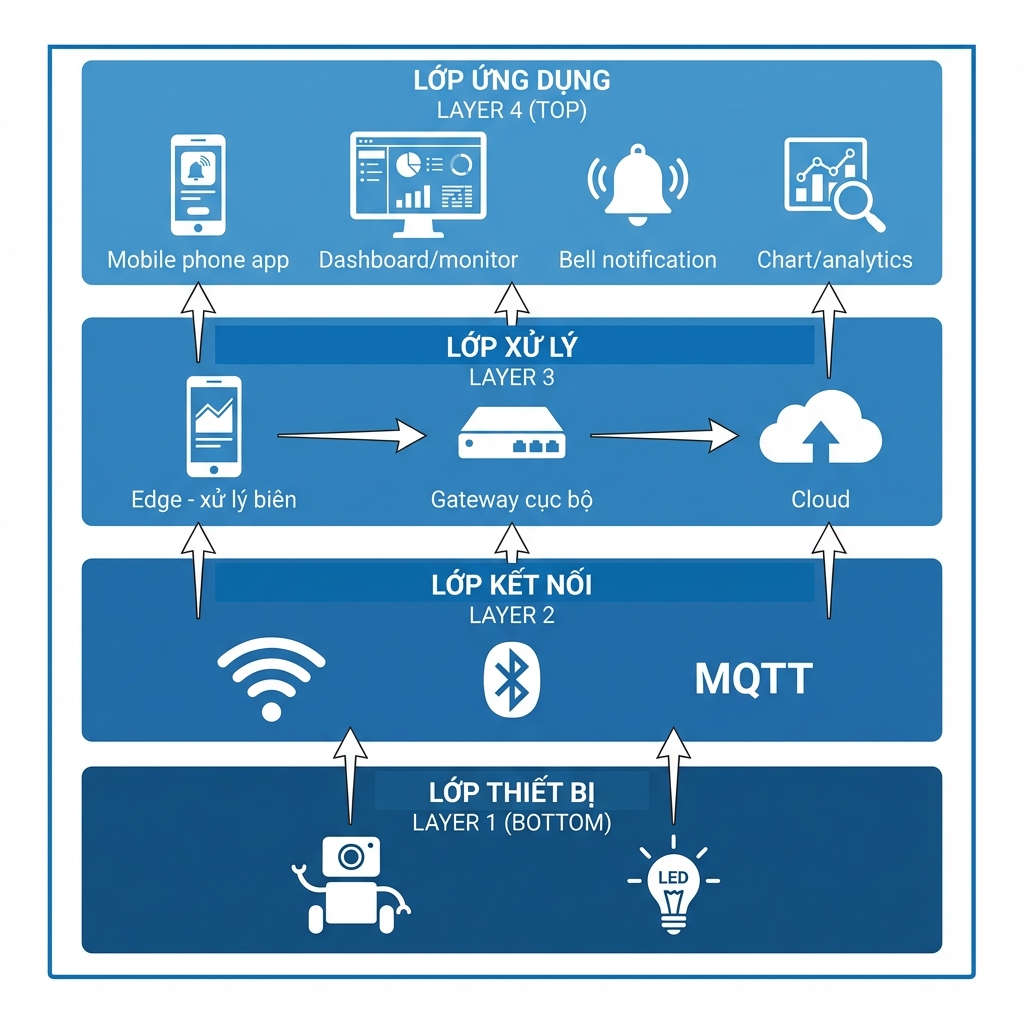
\includegraphics[width=0.85\textwidth]{Images/iot_architecture_layers.png}
%     \caption{Kiến trúc IoT 4 lớp cho hệ thống giám sát người cao tuổi}
%     \label{fig:iot_architecture}
% \end{figure}
% \newpage
% \textbf{a) Lớp Thiết bị (Device Layer)}

% Lớp thiết bị là tầng thấp nhất trong kiến trúc IoT, bao gồm các thiết bị vật lý trực tiếp tương tác với môi trường và người dùng:

% \begin{itemize}
%     \item \textbf{Robot}: Nền tảng OpenBot với khả năng di chuyển tự động, camera tích hợp để thu thập video stream, và các cảm biến khoảng cách để tránh vật cản. Robot đóng vai trò là ``mắt và tai'' di động của hệ thống, có thể tuần tra và tiếp cận người cao tuổi khi cần thiết.
    
%     \item \textbf{Actuators}: Các thiết bị chấp hành bao gồm đèn LED thông minh để cảnh báo bằng ánh sáng (nhấp nháy khi phát hiện té ngã), loa để phát thông báo bằng giọng nói (nhắc uống thuốc, cảnh báo nguy hiểm). Các actuator này được điều khiển qua giao thức MQTT, cho phép phản hồi nhanh trong các tình huống khẩn cấp.
% \end{itemize}

% \textbf{b) Lớp Kết nối (Connectivity Layer)}

% Lớp kết nối đảm bảo việc truyền dữ liệu giữa các thiết bị và hệ thống xử lý. Các giao thức được lựa chọn dựa trên yêu cầu về băng thông, độ trễ và tiêu thụ năng lượng:

% \begin{itemize}
%     \item \textbf{WiFi (IEEE 802.11)}: Giao thức kết nối chính cho smartphone (bộ não robot) và các thiết bị IoT với cloud. WiFi cung cấp băng thông cao (đủ cho video streaming) và được hỗ trợ rộng rãi trong môi trường gia đình. Smartphone kết nối qua WiFi để gửi video stream, nhận lệnh điều khiển, và đồng bộ dữ liệu với cloud.
    
%     \item \textbf{Bluetooth/BLE (Bluetooth Low Energy)}: Sử dụng cho kết nối tầm ngắn giữa smartphone và phần cứng robot (thay thế USB khi cần wireless), cũng như kết nối với các thiết bị đeo thông minh của người cao tuổi (vòng tay đo nhịp tim, nút bấm SOS). BLE tiêu thụ năng lượng thấp, phù hợp cho các thiết bị chạy pin.
    
%     \item \textbf{MQTT (Message Queuing Telemetry Transport)}: Giao thức nhắn tin publish-subscribe được thiết kế đặc biệt cho IoT. MQTT có header nhỏ (chỉ 2 bytes), phù hợp cho mạng có băng thông hạn chế và thiết bị tài nguyên thấp. Trong hệ thống, MQTT được sử dụng để:
%     \begin{itemize}
%         \item Gửi lệnh điều khiển từ ứng dụng người thân đến robot
%         \item Phát cảnh báo té ngã từ robot đến tất cả subscriber
%         \item Đồng bộ trạng thái thiết bị IoT (đèn, cửa, cảm biến)
%         \item Gửi heartbeat để giám sát trạng thái online của thiết bị
%     \end{itemize}
% \end{itemize}

% \textbf{c) Lớp Xử lý (Processing Layer)}

% Lớp xử lý đảm nhận việc phân tích dữ liệu và ra quyết định. Hệ thống áp dụng mô hình xử lý phân tán để tối ưu hóa độ trễ và chi phí:

% \begin{itemize}
%     \item \textbf{Edge Computing}: Xử lý trực tiếp trên smartphone (bộ não robot) với các tác vụ yêu cầu phản hồi real-time. Bao gồm:
%     \begin{itemize}
%         \item Chạy mô hình YOLOv11n để phát hiện té ngã với độ trễ $<$100ms
%         \item Xử lý ByteTrack để theo dõi người liên tục
%         \item Nhận diện giọng nói cục bộ (Vosk offline mode)
%         \item Điều khiển motor và phản hồi ngay lập tức
%     \end{itemize}
    
%     \item \textbf{Fog Computing}: Xử lý tại gateway cục bộ (có thể là router thông minh hoặc mini PC trong nhà) cho các tác vụ không yêu cầu phản hồi tức thì nhưng cần xử lý trước khi gửi lên cloud:
%     \begin{itemize}
%         \item Tổng hợp dữ liệu từ nhiều nguồn cảm biến
%         \item Cache video clips trước khi upload
%         \item Xử lý rule-based automation (bật đèn khi phát hiện chuyển động ban đêm)
%     \end{itemize}
    
%     \item \textbf{Cloud Computing}: Xử lý các tác vụ nặng và lưu trữ dài hạn trên cloud server:
%     \begin{itemize}
%         \item Chạy LLM API (GPT-4o, Gemini) cho chatbot thông minh
%         \item Lưu trữ lịch sử hoạt động và video clips
%         \item Huấn luyện và cập nhật mô hình AI
%         \item Phân tích pattern dài hạn để phát hiện bất thường
%     \end{itemize}
% \end{itemize}

% \textbf{d) Lớp Ứng dụng (Application Layer)}

% Lớp ứng dụng cung cấp giao diện người dùng và các tính năng cao cấp của hệ thống:

% \begin{itemize}
%     \item \textbf{Dashboard giám sát thời gian thực}: Giao diện web hiển thị trạng thái hệ thống, vị trí robot, video stream trực tiếp, và các cảnh báo. Dashboard cho phép người quản trị theo dõi nhiều thiết bị cùng lúc và can thiệp khi cần thiết.
    
%     \item \textbf{Ứng dụng mobile cho người chăm sóc}: Ứng dụng Android/iOS cho phép người thân:
%     \begin{itemize}
%         \item Nhận push notification khi phát hiện té ngã
%         \item Xem video stream từ robot theo thời gian thực
%         \item Điều khiển robot từ xa bằng virtual joystick
%         \item Thiết lập lịch nhắc uống thuốc và theo dõi tuân thủ
%         \item Thực hiện video call với người cao tuổi qua robot
%     \end{itemize}
    
%     \item \textbf{Hệ thống cảnh báo tự động}: Khi phát hiện sự cố (té ngã, bất động quá lâu, người lạ xâm nhập), hệ thống tự động:
%     \begin{itemize}
%         \item Phát cảnh báo âm thanh và ánh sáng tại chỗ
%         \item Gửi push notification đến tất cả người thân đã đăng ký
%         \item Lưu video clip trước và sau sự cố
%         \item Nếu không có phản hồi sau 2 phút, tự động gọi số khẩn cấp
%     \end{itemize}
    
%     \item \textbf{Phân tích dữ liệu và báo cáo}: Hệ thống tổng hợp dữ liệu hoạt động hàng ngày để:
%     \begin{itemize}
%         \item Tạo báo cáo tuân thủ uống thuốc (tuần/tháng)
%         \item Phân tích pattern hoạt động để phát hiện thay đổi bất thường
%         \item Thống kê thời gian hoạt động và nghỉ ngơi
%         \item Cung cấp insights cho bác sĩ hoặc người chăm sóc chuyên nghiệp
%     \end{itemize}
% \end{itemize}
% \subsubsection{Giao thức MQTT}

% MQTT (Message Queuing Telemetry Transport) là giao thức nhắn tin publish-subscribe được thiết kế cho IoT với các đặc điểm:

% \begin{itemize}
%     \item \textbf{Nhẹ}: Header tối thiểu 2 bytes, phù hợp thiết bị hạn chế tài nguyên
%     \item \textbf{Pub/Sub}: Mô hình publish-subscribe linh hoạt
%     \item \textbf{QoS}: Ba mức chất lượng dịch vụ (0, 1, 2)
%     \item \textbf{Retained Messages}: Lưu tin nhắn cuối cho subscriber mới
% \end{itemize}



\subsection{Giới thiệu YOLO (You Only Look Once)}
%=========================================

\subsubsection{Bài toán Object Detection}

Object Detection (Phát hiện đối tượng) là một trong những bài toán cơ bản và quan trọng nhất trong thị giác máy tính \reportcite{ref:odsurvey}. Khác với Image Classification chỉ xác định loại đối tượng chính trong ảnh, Object Detection yêu cầu đồng thời:

\begin{itemize}
    \item \textbf{Định vị (Localization)}: Xác định vị trí của đối tượng trong ảnh thông qua bounding box (hộp giới hạn)
    \item \textbf{Phân loại (Classification)}: Xác định loại của mỗi đối tượng được phát hiện
\end{itemize}

Trong bài toán phát hiện ngã, Object Detection đóng vai trò then chốt: mô hình cần xác định vị trí con người trong khung hình và phân loại trạng thái của họ (đang đứng, đi lại, hay đã ngã).

\subsubsection{Lịch sử phát triển Object Detection}

Theo khảo sát ``Object Detection in 20 Years'' của Zou và cộng sự \reportcite{ref:odsurvey}, lĩnh vực Object Detection đã trải qua sự phát triển đáng kể trong hơn hai thập kỷ:

\textbf{a) Giai đoạn truyền thống (1990s-2012)}

\begin{itemize}
    \item \textbf{Viola-Jones Detector (2001)}: Detector đầu tiên đạt tốc độ real-time cho face detection, sử dụng Haar-like features và AdaBoost
    \item \textbf{HOG Detector (2005)}: Histogram of Oriented Gradients cho pedestrian detection
    \item \textbf{DPM - Deformable Parts Model (2010)}: Mô hình biến dạng các phần, đạt SOTA trên PASCAL VOC nhiều năm
\end{itemize}

\textbf{b) Giai đoạn Deep Learning (2012-nay)}

\begin{itemize}
    \item \textbf{AlexNet (2012)}: Bước ngoặt của deep learning trong computer vision
    \item \textbf{R-CNN (2014)}: Kết hợp region proposals với CNN features
    \item \textbf{Fast R-CNN, Faster R-CNN (2015)}: Cải tiến tốc độ với RoI pooling và Region Proposal Network
    \item \textbf{YOLO v1 (2016)}: Đột phá với one-stage detection, real-time
    \item \textbf{SSD (2016)}: Single Shot MultiBox Detector với multi-scale features
    \item \textbf{RetinaNet (2017)}: Giới thiệu Focal Loss để giải quyết class imbalance
    \item \textbf{YOLO v3-v11 (2018-2024)}: Liên tục cải tiến về accuracy và speed
\end{itemize}

\textbf{c) Xu hướng hiện tại}

Theo \reportcite{ref:odsurvey}, các xu hướng chính trong Object Detection bao gồm:
\begin{itemize}
    \item Anchor-free detectors (loại bỏ anchor boxes)
    \item Transformer-based detectors (DETR, Swin Transformer)
    \item NAS-based architecture search (tự động tìm kiếm kiến trúc)
    \item Real-time detection trên edge devices
\end{itemize}

\subsubsection{Khái niệm Bounding Box}

Bounding Box (hộp giới hạn) là hình chữ nhật bao quanh đối tượng trong ảnh, được sử dụng để xác định vị trí và kích thước của đối tượng.

\begin{figure}[h!]
    \centering
    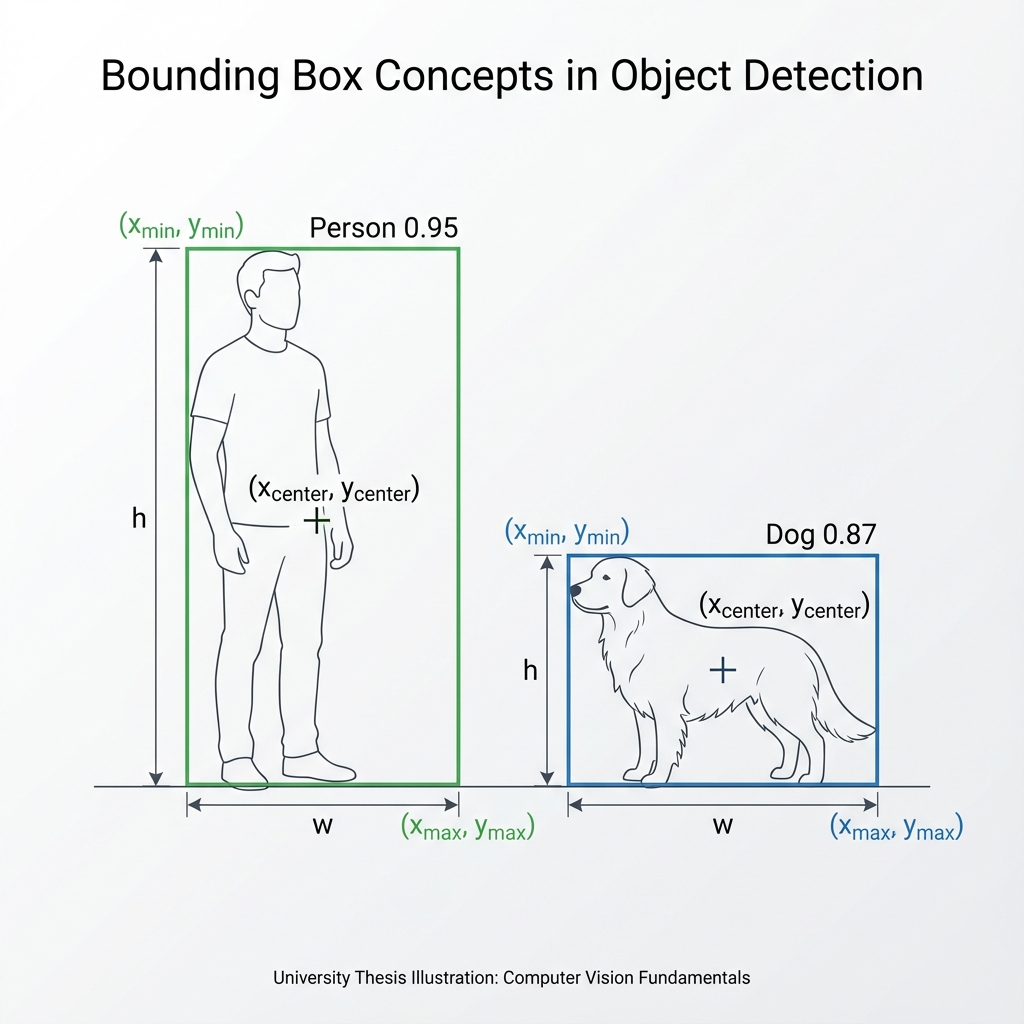
\includegraphics[width=0.6\textwidth]{Images/bounding_box_example.png}
    \vspace{8pt}
    \caption{Ví dụ minh họa Bounding Box trong Object Detection.}
    \label{fig:bounding_box}
\end{figure}

Có hai cách biểu diễn bounding box phổ biến:

\textbf{a) Format $(x_{min}, y_{min}, x_{max}, y_{max})$ - PASCAL VOC format}

\begin{itemize}
    \item $(x_{min}, y_{min})$: Tọa độ góc trên bên trái của box
    \item $(x_{max}, y_{max})$: Tọa độ góc dưới bên phải của box
    \item Đơn vị: pixel tuyệt đối
\end{itemize}

\textbf{b) Format $(x_{center}, y_{center}, w, h)$ - YOLO format}

\begin{itemize}
    \item $(x_{center}, y_{center})$: Tọa độ tâm của box
    \item $w$: Chiều rộng của box
    \item $h$: Chiều cao của box
    \item Đơn vị: normalized (chia cho kích thước ảnh, giá trị từ 0 đến 1)
\end{itemize}

\textbf{c) Công thức chuyển đổi}

Từ PASCAL VOC sang YOLO (với ảnh kích thước $W \times H$):
\begin{equation}
x_{center} = \frac{x_{min} + x_{max}}{2W}, \quad y_{center} = \frac{y_{min} + y_{max}}{2H}
\end{equation}
\begin{equation}
w = \frac{x_{max} - x_{min}}{W}, \quad h = \frac{y_{max} - y_{min}}{H}
\end{equation}

\subsubsection{Intersection over Union (IoU)}

IoU là metric đo độ chồng lấp giữa hai bounding box, được sử dụng rộng rãi trong đánh giá object detection:

\begin{equation}
IoU = \frac{\text{Area of Intersection}}{\text{Area of Union}} = \frac{|A \cap B|}{|A \cup B|}
\end{equation}

Trong đó:
\begin{itemize}
    \item $A$: Bounding box dự đoán (predicted)
    \item $B$: Bounding box ground truth (thực tế)
    \item IoU = 1: Hai box trùng khớp hoàn toàn
    \item IoU = 0: Hai box không có phần giao nhau
\end{itemize}

Ngưỡng IoU thường được sử dụng để xác định dự đoán đúng:
\begin{itemize}
    \item IoU $\geq 0.5$: Ngưỡng phổ biến (PASCAL VOC, COCO mAP@0.5)
    \item IoU $\geq 0.75$: Ngưỡng nghiêm ngặt (COCO mAP@0.75)
    \item IoU từ 0.5 đến 0.95: Đánh giá đa ngưỡng (COCO mAP@[.5:.95])
\end{itemize}

\subsubsection{Các khái niệm True Positive, False Positive, False Negative}

Để đánh giá kết quả detection, cần phân loại các dự đoán:

\begin{itemize}
    \item \textbf{True Positive (TP)}: Dự đoán đúng - có bounding box dự đoán khớp với ground truth (IoU $\geq$ threshold) và đúng class
    \item \textbf{False Positive (FP)}: Dự đoán sai - bounding box dự đoán không khớp với bất kỳ ground truth nào, hoặc sai class
    \item \textbf{False Negative (FN)}: Bỏ sót - ground truth không được detect bởi bất kỳ dự đoán nào
\end{itemize}

Từ đó tính được:
\begin{equation}
\text{Precision} = \frac{TP}{TP + FP} = \frac{\text{Số dự đoán đúng}}{\text{Tổng số dự đoán}}
\end{equation}
\begin{equation}
\text{Recall} = \frac{TP}{TP + FN} = \frac{\text{Số dự đoán đúng}}{\text{Tổng số ground truth}}
\end{equation}

\subsubsection{Đánh giá hiệu suất: Mean Average Precision (mAP)}

Mean Average Precision (mAP) là metric chuẩn để đánh giá hiệu suất của mô hình object detection, tổng hợp cả precision và recall.

\textbf{a) Precision-Recall Curve}

Với mỗi class, sắp xếp các dự đoán theo confidence score giảm dần. Tại mỗi điểm, tính precision và recall tích lũy, từ đó vẽ được đường cong Precision-Recall.

\textbf{b) Average Precision (AP)}

AP là diện tích dưới đường cong Precision-Recall:
\begin{equation}
AP = \int_0^1 p(r) \, dr
\end{equation}

Trong thực tế, sử dụng phép nội suy (interpolation):
\begin{equation}
AP = \sum_{i=1}^{n} (r_i - r_{i-1}) \cdot p_{interp}(r_i)
\end{equation}

với $p_{interp}(r) = \max_{r' \geq r} p(r')$ là precision nội suy tại recall $r$.

\textbf{c) Mean Average Precision (mAP)}

mAP là trung bình của AP trên tất cả các class:
\begin{equation}
mAP = \frac{1}{N} \sum_{i=1}^{N} AP_i
\end{equation}

với $N$ là số class trong dataset.

\textbf{d) Các biến thể mAP}

\begin{itemize}
    \item \textbf{mAP@0.5 (mAP50)}: AP tính với ngưỡng IoU = 0.5, được sử dụng trong PASCAL VOC
    \item \textbf{mAP@0.75 (mAP75)}: AP với ngưỡng IoU = 0.75, nghiêm ngặt hơn
    \item \textbf{mAP@[.5:.95]}: Trung bình AP với IoU từ 0.5 đến 0.95 (bước 0.05), metric chính của COCO
    \item \textbf{mAP Small/Medium/Large}: mAP theo kích thước đối tượng
\end{itemize}

\textbf{e) Ý nghĩa của mAP}

\begin{itemize}
    \item mAP cao $\rightarrow$ Mô hình phát hiện đúng nhiều đối tượng và định vị chính xác
    \item mAP50 cao nhưng mAP75 thấp $\rightarrow$ Phát hiện được nhưng định vị chưa chính xác
    \item Precision cao, Recall thấp $\rightarrow$ Mô hình thận trọng, ít false positive nhưng bỏ sót nhiều
    \item Precision thấp, Recall cao $\rightarrow$ Mô hình phát hiện nhiều nhưng có nhiều false positive
\end{itemize}

\subsubsection{Ý tưởng YOLO: Phát hiện trong một lần suy luận}

YOLO (You Only Look Once) được Joseph Redmon, Santosh Divvala, Ross Girshick và Ali Farhadi đề xuất năm 2016 trong bài báo ``You Only Look Once: Unified, Real-Time Object Detection'' \reportcite{ref:yolo}. Đây là bước đột phá mang đến cách tiếp cận hợp nhất cho Object Detection.

\textbf{Ý tưởng cốt lõi của YOLO} (theo \reportcite{ref:yolo}):

``We reframe object detection as a single regression problem, straight from image pixels to bounding box coordinates and class probabilities. Using our system, you only look once (YOLO) at an image to predict what objects are present and where they are.''

Thay vì coi detection như bài toán phân loại (classifier), YOLO đặt lại vấn đề như bài toán hồi quy về tọa độ bounding box và xác suất class, tất cả trong một lần forward pass duy nhất qua mạng neural.

\textbf{Nguyên lý hoạt động của YOLO:}

\begin{enumerate}
    \item \textbf{Chia lưới}: Ảnh đầu vào được chia thành lưới $S \times S$ ô (grid cells). Trong paper gốc, $S = 7$.

    \begin{figure}[h!]
        \centering
        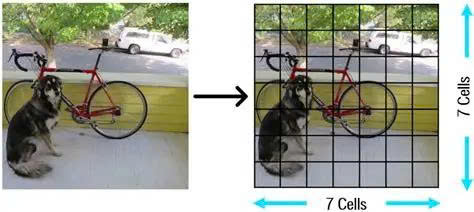
\includegraphics[width=0.7\textwidth]{Images/7x7.jpg}
        \vspace{8pt}
        \caption{Minh họa chia lưới $7 \times 7$ trong YOLO: mỗi ô chịu trách nhiệm phát hiện đối tượng có tâm nằm trong ô đó.}
        \label{fig:yolo_grid}
    \end{figure}
    \item \textbf{Dự đoán bounding boxes}: Mỗi ô dự đoán $B$ bounding boxes (mặc định $B = 2$) cùng với điểm confidence.
    \item \textbf{Dự đoán class probabilities}: Mỗi ô dự đoán $C$ xác suất class có điều kiện $Pr(Class_i|Object)$.
    \item \textbf{Tensor đầu ra}: Kích thước $S \times S \times (B \times 5 + C)$. Với PASCAL VOC ($C=20$), tensor có kích thước $7 \times 7 \times 30$.
    \item \textbf{Post-processing}: Non-Maximum Suppression (NMS) loại bỏ các box trùng lặp.
\end{enumerate}

\textbf{Đầu ra của mỗi bounding box bao gồm 5 giá trị:}
\begin{itemize}
    \item $(x, y)$: Tọa độ tâm của box tương đối với ô lưới (normalized 0-1 trong ô)
    \item $(w, h)$: Chiều rộng và chiều cao của box tương đối với toàn ảnh (normalized 0-1)
    \item $confidence = Pr(Object) \times IOU^{truth}_{pred}$: Độ tin cậy rằng box chứa đối tượng VÀ độ chính xác của box so với ground truth
\end{itemize}

\textbf{Hiệu suất của YOLO theo bài báo gốc:}
\begin{itemize}
    \item Base YOLO: 45 FPS (frames per second) trên GPU
    \item Fast YOLO: 155 FPS - nhanh hơn gấp đôi các detector real-time khác
    \item mAP trên PASCAL VOC 2007: 63.4\% (base), 52.7\% (fast)
\end{itemize}

\subsubsection{So sánh YOLO với phương pháp truyền thống}

\begin{table}[h]
\centering
\caption{So sánh YOLO với các phương pháp Object Detection khác}
\begin{tabular}{|l|c|c|c|}
\hline
\textbf{Phương pháp} & \textbf{Tốc độ (FPS)} & \textbf{mAP} & \textbf{Thời gian thực} \\
\hline
R-CNN & 0.02 & 53.7 & Không \\
Fast R-CNN & 0.5 & 70.0 & Không \\
Faster R-CNN & 7-17 & 73.2 & Khó \\
YOLO v1 & 45 & 63.4 & Có \\
YOLOv3 & 30-50 & 57.9 & Có \\
YOLOv5 & 100+ & 68.9 & Có \\
\hline
\end{tabular}
\end{table}

\textbf{Ưu điểm của YOLO:}
\begin{itemize}
    \item Tốc độ: Xử lý real-time với hàng chục đến hàng trăm FPS
    \item Đơn giản: Một mạng duy nhất, dễ huấn luyện end-to-end
    \item Nhìn toàn cục: Xem xét toàn bộ ảnh khi dự đoán, hiểu được ngữ cảnh tốt hơn
    \item Tổng quát hóa tốt: Ít false positive trên background so với các phương pháp dựa trên sliding window
\end{itemize}

\textbf{Hạn chế:}
\begin{itemize}
    \item Khó phát hiện các đối tượng nhỏ hoặc xếp chồng nhau
    \item Độ chính xác định vị có thể kém hơn phương pháp hai giai đoạn ở một số trường hợp
\end{itemize}

%=========================================
\subsection{Nền tảng Thị giác máy tính (Computer Vision)}

Thị giác máy tính (Computer Vision) đóng vai trò cốt lõi trong hệ thống giám sát và nhận diện té ngã. Bằng cách phân tích luồng video từ camera, hệ thống có khả năng nhận biết, định vị và theo dõi con người trong không gian. Phần này trình bày các nền tảng kỹ thuật được sử dụng bao gồm Mạng nơ-ron tích chập (CNN), kiến trúc YOLO cho bài toán phát hiện đối tượng và thuật toán ByteTrack cho bài toán theo dõi.

\subsubsection{Mạng nơ-ron tích chập (CNN) và Kiến trúc YOLO26}

\textbf{Mạng nơ-ron tích chập (CNN)}

Mạng nơ-ron tích chập (Convolutional Neural Network - CNN) là một lớp mạng học sâu (Deep Learning) chuyên biệt, được thiết kế để xử lý dữ liệu có dạng lưới tĩnh như hình ảnh 2D
\reportcite{ref:cnn}. Khác với mạng đa tầng (MLP) truyền thống yêu cầu làm phẳng (flatten) hình ảnh gây mất thông tin không gian, CNN bảo toàn cấu trúc không gian của pixel bằng cách sử dụng các bộ lọc (filters/kernels) trượt qua toàn bộ bức ảnh.

Kiến trúc cốt lõi của một mạng CNN tiêu chuẩn bao gồm 3 loại lớp chính:
\begin{itemize}
    \item \textbf{Lớp tích chập (Convolutional Layer)}: Đóng vai trò là bộ trích xuất đặc trưng (feature extractor). Nó áp dụng các phép tính tích chập giữa một bộ lọc ma trận (kernel) và vùng ảnh đầu vào để tạo ra các bản đồ đặc trưng (feature maps). Ở các lớp đầu, CNN học cách nhận diện các đặc trưng cấp thấp như cạnh, góc; ở các lớp sâu hơn, nó nhận diện các đặc trưng phức tạp như hình khối, khuôn mặt.
    \item \textbf{Lớp gộp (Pooling Layer)}: Thường theo ngay sau lớp tích chập (như Max Pooling hoặc Average Pooling), có nhiệm vụ giảm độ phân giải không gian của bản đồ đặc trưng. Quá trình này không chỉ giúp giảm đáng kể khối lượng tính toán, tránh hiện tượng quá khớp (overfitting) mà còn mang lại tính bất biến cục bộ (translation invariance) -- giúp mô hình vẫn nhận diện được đối tượng dù chúng bị dịch chuyển nhẹ trong khung hình.
    \item \textbf{Lớp kết nối đầy đủ (Fully Connected Layer)}: Nằm ở phần cuối mạng, làm nhiệm vụ tổng hợp các đặc trưng cao cấp đã được trích xuất để thực hiện dự đoán cuối cùng (phân loại hoặc hồi quy tọa độ).
\end{itemize}

Bên cạnh đó, sau mỗi lớp tích chập, một hàm kích hoạt phi tuyến (như ReLU, SiLU) được áp dụng để đưa tính phi tuyến vào mô hình, cho phép CNN học được các mối quan hệ phức tạp. Sự kết hợp luân phiên giữa Convolution và Pooling giúp CNN tự động học cách phân tích hình ảnh mà không cần đến các chuyên gia thiết kế đặc trưng thủ công (manual feature engineering) như các phương pháp thị giác máy tính cổ điển.

\begin{figure}[htbp]
    \centering
    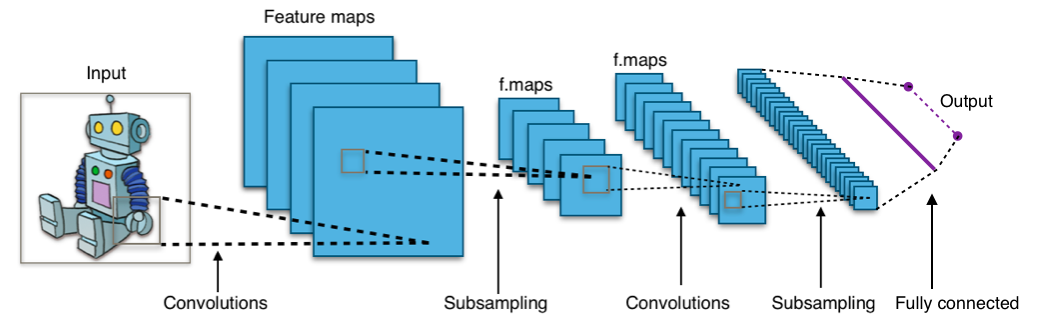
\includegraphics[width=0.9\textwidth]{Images/cnn_arch.png}
    \caption{Minh họa cấu trúc tiêu biểu của mạng nơ-ron tích chập (CNN) gồm các lớp Convolution, Pooling và Fully Connected.}
    \label{fig:typical_cnn}
\end{figure}

\textbf{Kiến trúc YOLO26 (Kế thừa từ YOLOv8/YOLOv11)}
YOLO (You Only Look Once) là một trong những họ mô hình Object Detection tốc độ cao phổ biến nhất. Khác với các phương pháp dựa trên region-proposal (như Faster R-CNN) yêu cầu chạy mô hình nhiều lần trên một ảnh, YOLO định hình bài toán detection như một bài toán hồi quy đơn lẻ (single regression problem) dự đoán trực tiếp tọa độ Bounding Box và xác suất nhãn lớp từ các pixel hình ảnh trong một lần quét duy nhất
\reportcite{ref:yolo}.

Trong hệ thống, mô hình YOLO26 (phiên bản nano tối ưu từ YOLO-Pose) được sử dụng nhằm mục đích trích xuất khung xương (pose landmarks) thay vì chỉ lấy bounding box thông thường.
Mô hình này nổi bật với các cải tiến kiến trúc như:
\begin{itemize}
    \item \textbf{Backbone hiệu năng cao}: Sử dụng các khối C3k2 (Cross Stage Partial) giúp giảm tham số nhưng vẫn duy trì độ chính xác cao.
    \item \textbf{Đầu ra đa nhiệm (Multi-task Head)}: Hỗ trợ dự đoán đồng thời vị trí Bounding Box và 17 điểm khớp xương (keypoints) của con người.
    \item \textbf{Tối ưu hóa cho thiết bị biên (Edge Devices)}: Phiên bản nano (yolo26n-pose) có dung lượng cực nhẹ, phù hợp để chuyển đổi sang định dạng TFLite hoặc ONNX, giúp hệ thống đạt tốc độ Real-time trên các phần cứng hạn chế như Raspberry Pi hay điện thoại di động.
\end{itemize}

\begin{figure}[htbp]
    \centering
    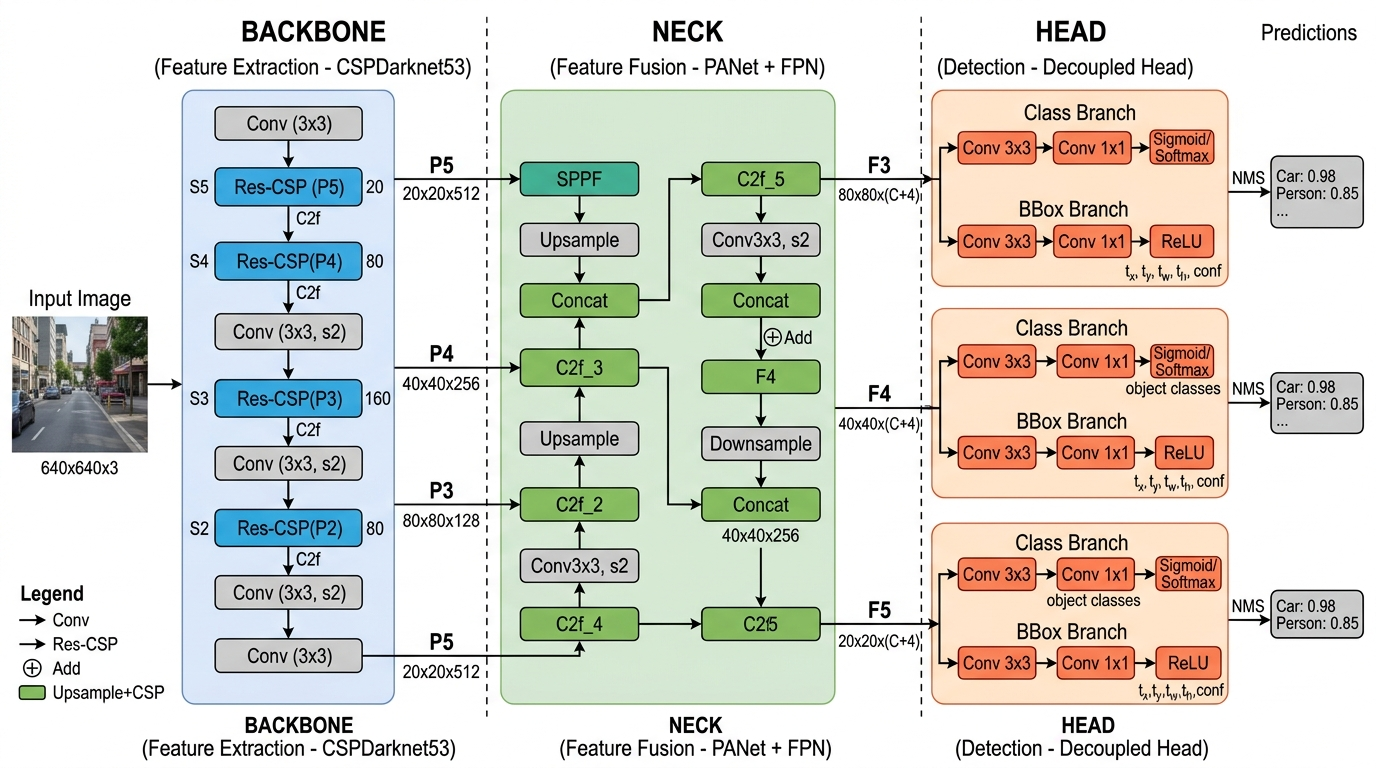
\includegraphics[width=0.8\textwidth]{yolo_arch.jpg}
    \caption{Minh họa một kiến trúc mạng YOLO tiêu biểu với Backbone, Neck và Head.}
    \label{fig:yolo_architecture}
\end{figure}

\subsubsection{Thuật toán theo dõi đa đối tượng ByteTrack}

Trong bài toán nhận diện té ngã, không chỉ cần phát hiện người ở từng khung hình (frame) riêng lẻ, mà còn phải liên kết các phát hiện đó xuyên suốt thời gian để tạo thành một chuỗi hành động (tracklet). Đây là vai trò của bài toán Theo dõi đa đối tượng (Multi-Object Tracking - MOT).

Hệ thống ứng dụng thuật toán \textbf{ByteTrack}, một trong những thuật toán tracking State-of-the-Art hiện nay với phương pháp tiếp cận độc đáo về ghép nối dữ liệu (data association)
\reportcite{ref:bytetrack}.

\textbf{Cơ chế hoạt động của ByteTrack:}
Các thuật toán tracking truyền thống thường loại bỏ hoàn toàn các detection có độ tin cậy thấp (low-confidence) nhằm giảm thiểu nhiễu. Tuy nhiên, điều này dẫn đến việc mất dấu đối tượng khi họ bị che khuất một phần (occlusion) hoặc hình ảnh bị mờ do chuyển động nhanh (thường gặp khi nạn nhân đang ngã).

ByteTrack giải quyết vấn đề này bằng kỹ thuật \textbf{Dual-threshold Association} (Liên kết hai ngưỡng):
\begin{enumerate}
    \item \textbf{Ghép nối lần 1 (High-score association)}: Thuật toán sử dụng bộ lọc Kalman (Kalman Filter) để dự đoán vị trí của đối tượng ở frame tiếp theo. Sau đó, nó tính toán khoảng cách IoU (Intersection over Union) giữa vị trí dự đoán và các bounding box có độ tin cậy \textit{cao} do YOLO trả về. Các cặp phù hợp sẽ được liên kết với nhau.
    \item \textbf{Ghép nối lần 2 (Low-score association)}: Đối với các đối tượng chưa tìm được ghép nối (unmatched tracks) ở lần 1, ByteTrack không xóa chúng đi mà tiếp tục tìm kiếm trong nhóm các bounding box có độ tin cậy \textit{thấp}. Nếu nạn nhân đang ngã bị mờ, YOLO có thể trả về box với độ tin cậy thấp. Nhờ bước thứ hai này, ByteTrack có thể "cứu" lại tracklet của nạn nhân, giúp chuỗi hành động không bị ngắt quãng.
\end{enumerate}

\begin{figure}[htbp]
    \centering
    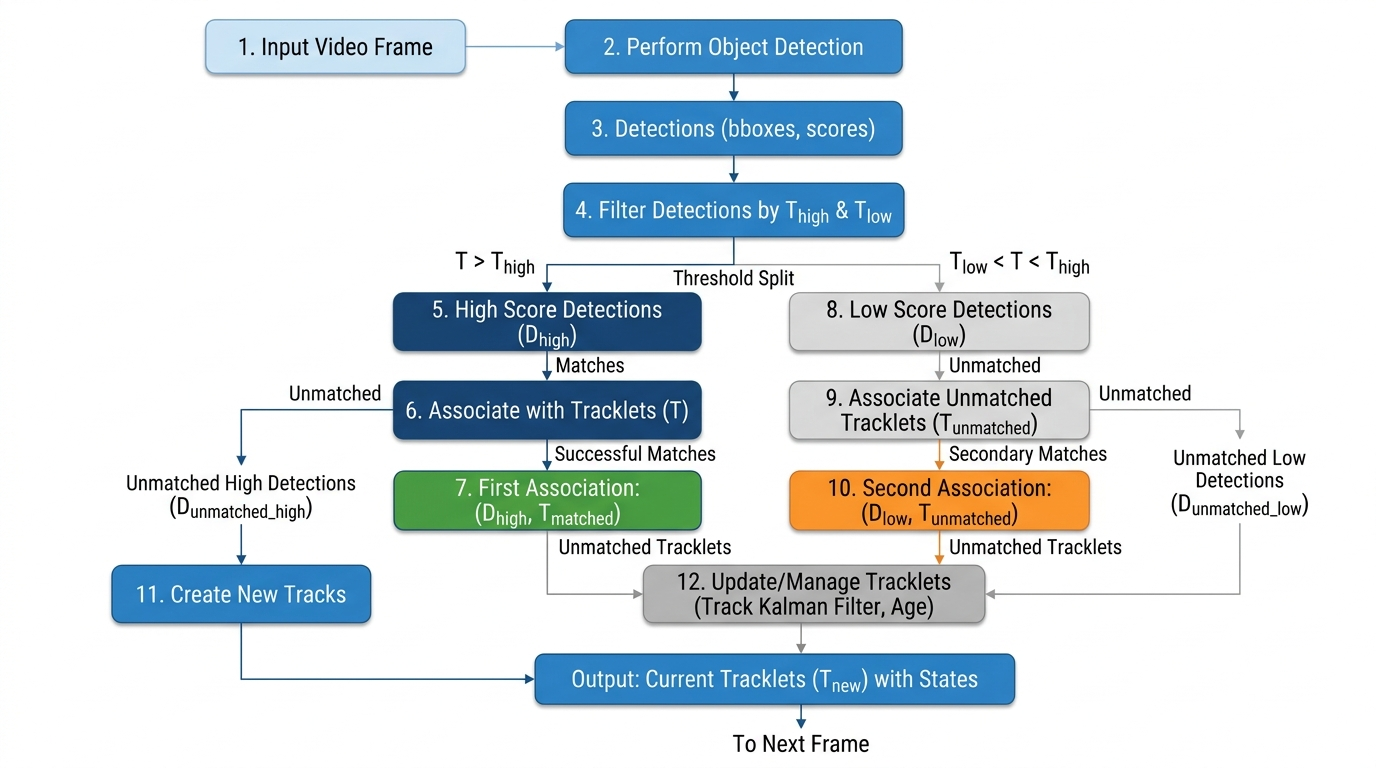
\includegraphics[width=0.9\textwidth]{bytetrack_arch.jpg}
    \caption{Thuật toán ByteTrack với cơ chế Dual-threshold Association giúp duy trì Track ID ổn định.}
    \label{fig:bytetrack}
\end{figure}

Sự kết hợp giữa YOLO26 (nhận diện chính xác, nhanh) và ByteTrack (liên kết mạnh mẽ, chống đứt gãy) tạo nên một nền tảng vững chắc để trích xuất dữ liệu chuỗi thời gian chất lượng cao, trước khi đưa vào mạng LSTM phân tích hành vi ngã.




% --- Tích hợp từ phần cũ ---

Tracking-by-detection tách bài toán thành phát hiện đối tượng ở mỗi frame và liên kết detection qua thời gian. SORT sử dụng Kalman để dự báo chuyển động, IoU làm độ tương đồng và Hungarian cho phép gán tối ưu \reportcite{ref:sort}. Deep SORT bổ sung embedding ngoại hình để giảm đổi ID khi che khuất \reportcite{ref:deepsort}; ByteTrack chỉ ra rằng các detection confidence thấp vẫn có thể hữu ích khi liên kết với track \reportcite{ref:bytetrack}.

Kalman gồm hai pha. Pha dự báo:

\begin{align}
\hat{x}_{t|t-1}&=F\hat{x}_{t-1|t-1}+Bu_t,\\
P_{t|t-1}&=FP_{t-1|t-1}F^T+Q.
\end{align}

Pha cập nhật với quan sát $z_t$:

\begin{align}
K_t&=P_{t|t-1}H^T(HP_{t|t-1}H^T+R)^{-1},\\
\hat{x}_{t|t}&=\hat{x}_{t|t-1}+K_t(z_t-H\hat{x}_{t|t-1}),\\
P_{t|t}&=(I-K_tH)P_{t|t-1}.
\end{align}

Ma trận chi phí giữa $n$ track và $m$ detection được đưa vào thuật toán Hungarian, vốn giải bài toán gán tuyến tính \reportcite{ref:hungarian}. IoU đơn độc có thể thất bại khi người từ đứng chuyển sang nằm làm vùng bao thay đổi mạnh. Vì vậy đề tài kết hợp IoU, khoảng cách tâm, neo vai/hông, tỷ lệ diện tích và histogram vùng thân. Định danh ID0 còn được bảo vệ bởi tuổi track dài hơn và phục hồi có điều kiện.


\subsection{Mô hình chuỗi thời gian (Sequence Modeling)}
%=========================================

\subsubsection{Mạng nơ-ron hồi quy (RNN)}

Mạng nơ-ron hồi quy (Recurrent Neural Network - RNN) là một lớp mạng nơ-ron nhân tạo chuyên biệt để xử lý dữ liệu dạng chuỗi (sequence data) như văn bản, âm thanh, hoặc chuỗi thời gian (time-series). Trong ngữ cảnh phát hiện té ngã, luồng video chứa các khung hình liên tiếp tạo thành một chuỗi dữ liệu thời gian ghi nhận chuyển động của con người
\reportcite{ref:rnn}.

Khác với mạng truyền thẳng (Feedforward Neural Network) nơi dữ liệu chỉ đi một chiều từ đầu vào đến đầu ra, RNN sở hữu các "vòng lặp" (loops) cho phép thông tin có thể lưu lại và truyền qua các bước thời gian.
Nhờ cơ chế trạng thái ẩn (hidden state), mạng RNN có thể nhớ được thông tin từ quá khứ để ảnh hưởng đến quyết định ở hiện tại. Tuy nhiên, RNN truyền thống gặp phải vấn đề \textbf{triệt tiêu đạo hàm (vanishing gradient)} và \textbf{bùng nổ đạo hàm (exploding gradient)} khi phải học các phụ thuộc xa (long-term dependencies) trong những chuỗi dữ liệu dài.

\subsubsection{Mạng Bộ nhớ Ngắn-Dài hạn (LSTM)}

Để khắc phục nhược điểm của RNN, mạng \textbf{Long Short-Term Memory (LSTM)} được đề xuất bởi Hochreiter và Schmidhuber (1997)
\reportcite{ref:lstm}. LSTM có khả năng học các phụ thuộc dài hạn cực kỳ xuất sắc nhờ cấu trúc "Cell State" (trạng thái tế bào) hoạt động như một băng chuyền thông tin xuyên suốt các bước thời gian, giúp đạo hàm không bị suy giảm quá nhanh.

Cốt lõi của kiến trúc LSTM nằm ở ba cổng (gates) đóng vai trò kiểm soát luồng thông tin:
\begin{itemize}
    \item \textbf{Cổng quên (Forget Gate)}: Quyết định lượng thông tin từ quá khứ (trạng thái tế bào trước đó) cần bị loại bỏ hoặc lãng quên.
    \item \textbf{Cổng đầu vào (Input Gate)}: Quyết định lượng thông tin mới (từ dữ liệu hiện tại và trạng thái ẩn trước đó) nào sẽ được cập nhật vào trạng thái tế bào.
    \item \textbf{Cổng đầu ra (Output Gate)}: Quyết định thông tin nào từ trạng thái tế bào sẽ được xuất ra dưới dạng trạng thái ẩn mới cho bước thời gian tiếp theo.
\end{itemize}

\begin{figure}[htbp]
    \centering
    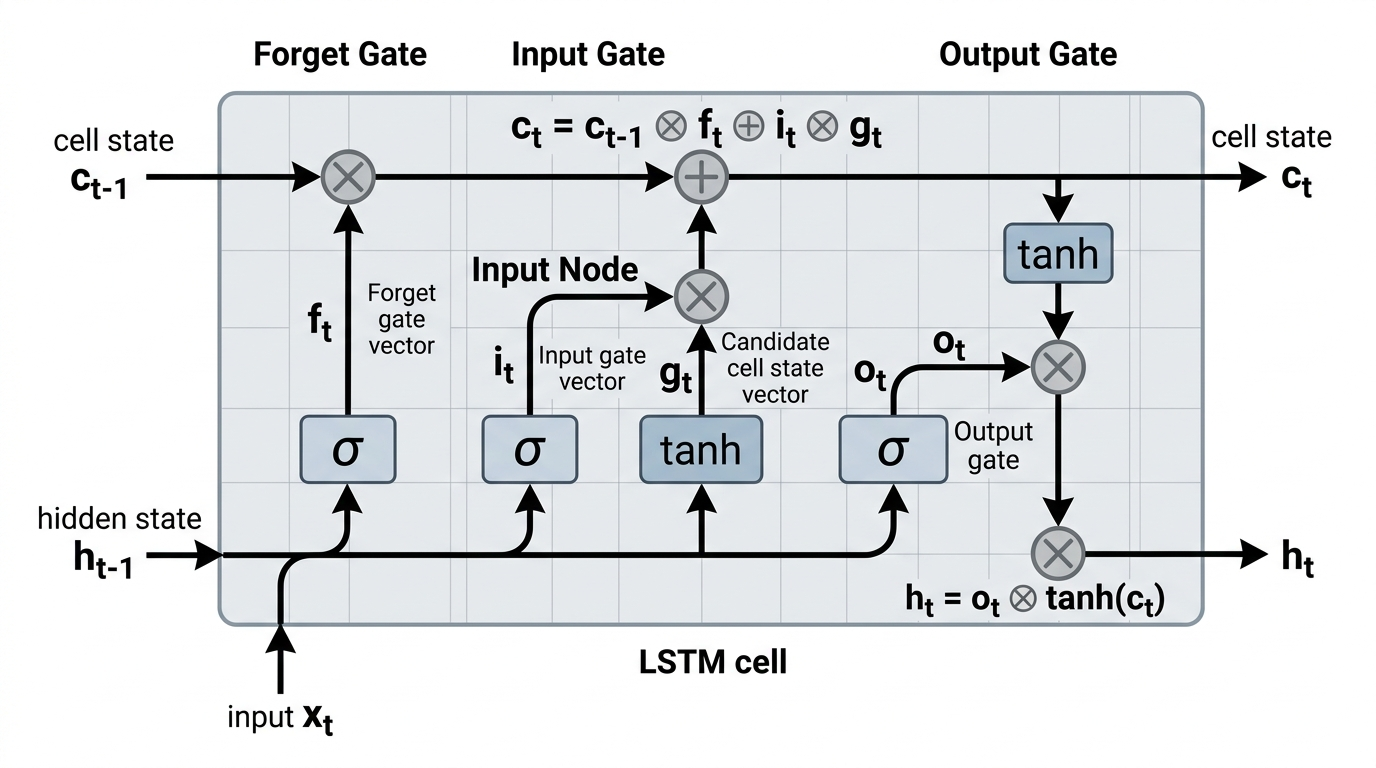
\includegraphics[width=0.9\textwidth]{Images/lstm_arch.jpg}
    \caption{Cấu trúc chi tiết của một tế bào LSTM (LSTM cell) với hệ thống các cổng kiểm soát thông tin.}
    \label{fig:lstm_architecture}
\end{figure}

Trong kiến trúc của hệ thống nhận diện té ngã, LSTM đóng vai trò cực kỳ quan trọng ở khâu cuối cùng. Sau khi mạng YOLO và thuật toán ByteTrack trích xuất ra một chuỗi các tọa độ điểm neo (keypoints) xuyên suốt các khung hình, dữ liệu này mang tính chất chuỗi thời gian. Mạng LSTM sẽ tiếp nhận chuỗi tọa độ này, phân tích sự thay đổi vị trí không gian của cơ thể con người theo thời gian, từ đó nhận diện được hành động ngã một cách chính xác so với các hành động bình thường như ngồi, cúi người hay nằm.



% --- Tích hợp từ phần cũ ---

Một detector trên từng ảnh chỉ quan sát tư thế tại một thời điểm. Trong bài toán té ngã, quá trình chuyển từ đứng/ngồi sang hạ thấp nhanh rồi nằm mới là tín hiệu quan trọng. Recurrent Neural Network (RNN) đưa trạng thái ẩn từ bước $t-1$ sang bước $t$, nhưng có thể gặp mất hoặc bùng nổ gradient khi chuỗi dài. Long Short-Term Memory (LSTM) bổ sung cell state và ba cổng vào, quên, ra để điều tiết thông tin \reportcite{ref:lstm}.

Với input $x_t$, hidden state $h_{t-1}$ và cell state $c_{t-1}$:

\begin{align}
f_t &= \sigma(W_f[x_t,h_{t-1}]+b_f),\\
i_t &= \sigma(W_i[x_t,h_{t-1}]+b_i),\\
\tilde{c}_t &= \tanh(W_c[x_t,h_{t-1}]+b_c),\\
c_t &= f_t\odot c_{t-1}+i_t\odot\tilde{c}_t,\\
o_t &= \sigma(W_o[x_t,h_{t-1}]+b_o),\\
h_t &= o_t\odot\tanh(c_t).
\end{align}

Trong hệ thống, một mẫu là tensor $X\in\mathbb{R}^{15\times69}$. Số 15 là chiều thời gian; 69 là vector pose/hình học mỗi frame. Đầu ra softmax hai lớp được diễn giải là normal/fall. Threshold xác suất chỉ là tầng đầu; hysteresis theo số frame liên tiếp và hậu kiểm hình học giúp ngăn trạng thái dao động. Cần lưu ý nếu FPS thay đổi, 15 frame tương ứng thời gian thực khác nhau; một triển khai tốt nên log timestamp hoặc resample chuỗi theo thời gian.


\subsection{Xử lý Ngôn ngữ Tự nhiên (NLP) và Hệ thống Giọng nói}
%=========================================

\subsubsection{Mô hình ngôn ngữ lớn (LLM) và Kiến trúc Transformer}

Mô hình ngôn ngữ lớn (Large Language Model - LLM) là một bước đột phá trong lĩnh vực Trí tuệ Nhân tạo, được huấn luyện trên lượng dữ liệu văn bản khổng lồ để có khả năng hiểu, suy luận và tạo ra ngôn ngữ tự nhiên giống con người. Trái tim của các mô hình LLM hiện đại chính là kiến trúc \textbf{Transformer} \reportcite{ref:transformer}.

Kiến trúc Transformer loại bỏ hoàn toàn cơ chế xử lý tuần tự của RNN/LSTM, thay vào đó sử dụng cơ chế \textbf{Tự chú ý (Self-Attention)}. Cơ chế này cho phép mô hình đánh giá mức độ liên quan (trọng số) của từng từ trong câu với tất cả các từ khác cùng một lúc, bất kể khoảng cách giữa chúng. Nhờ đó, Transformer không chỉ giải quyết triệt để vấn đề quên thông tin tầm xa mà còn hỗ trợ tính toán song song, giúp tăng tốc độ huấn luyện lên nhiều lần.

\begin{figure}[htbp]
    \centering
    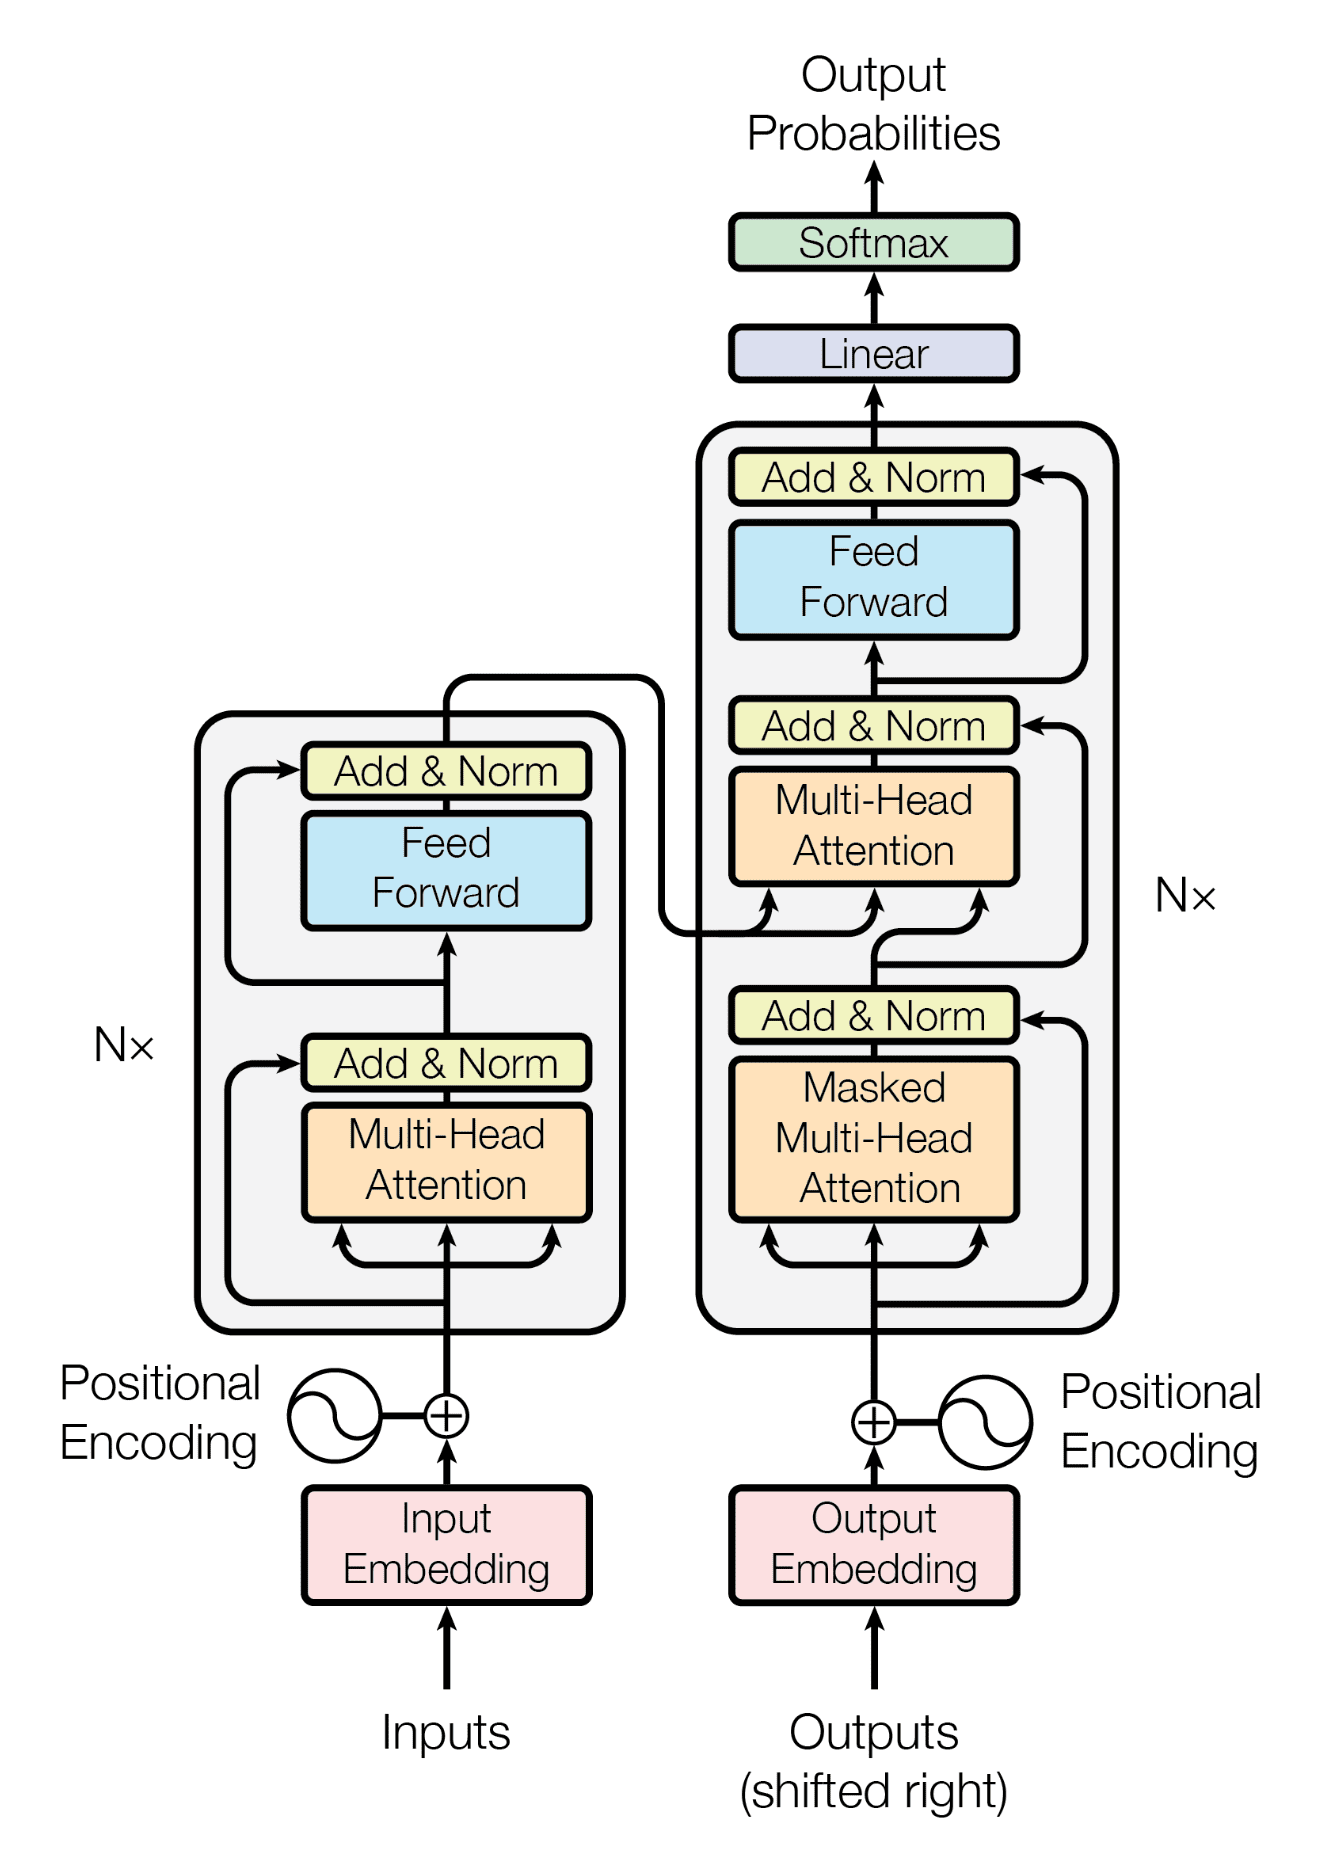
\includegraphics[width=0.6\textwidth]{Images/transformer_arch.png}
    \caption{Sơ đồ kiến trúc của mô hình Transformer với cơ chế Multi-Head Attention.}
    \label{fig:transformer}
\end{figure}

Trong phạm vi hệ thống robot hỗ trợ người cao tuổi, việc triển khai một mô hình LLM với hàng tỷ tham số trực tiếp trên phần cứng cục bộ (edge devices) là không khả thi do giới hạn về bộ nhớ và năng lượng. Do đó, hệ thống sử dụng \textbf{Groq API} để gọi các mô hình LLM mã nguồn mở (như LLaMA 3 hoặc Mixtral) thông qua điện toán đám mây \reportcite{ref:groq_api}. Điểm khác biệt của Groq là việc sử dụng chip LPU (Language Processing Unit) chuyên biệt cho inference, mang lại tốc độ phản hồi cực kỳ nhanh (có thể lên tới hàng trăm token/giây). Điều này rất quan trọng để đảm bảo robot có thể giao tiếp, nhắc nhở hoặc trò chuyện với người cao tuổi theo thời gian thực mà không có độ trễ gây khó chịu.


% --- Tích hợp từ phần cũ ---
%=========================================

\subsubsection{Khái niệm AI Agent}

AI Agent (Tác tử trí tuệ nhân tạo) là một hệ thống tự động có khả năng nhận thức môi trường, đưa ra quyết định, và thực hiện hành động để đạt được mục tiêu cụ thể. Khác với các chương trình truyền thống hoạt động theo luật cố định, AI Agent có khả năng:

\begin{itemize}
    \item \textbf{Tự chủ (Autonomy)}: Hoạt động độc lập mà không cần sự can thiệp liên tục của con người
    \item \textbf{Phản ứng (Reactivity)}: Nhận thức và phản hồi kịp thời với thay đổi của môi trường
    \item \textbf{Chủ động (Proactivity)}: Khởi xướng hành động để đạt mục tiêu, không chỉ phản ứng thụ động
    \item \textbf{Xã hội (Social ability)}: Tương tác và giao tiếp với con người hoặc các agent khác
\end{itemize}

Trong hệ thống robot giám sát người cao tuổi, AI Agent đóng vai trò là ``bộ não'' thông minh, điều phối các thành phần khác nhau (camera, cảm biến, IoT) và giao tiếp tự nhiên với người dùng.

\subsubsection{Mô hình Ngôn ngữ Lớn (Large Language Models)}

Large Language Models (LLM) là các mô hình học sâu được huấn luyện trên lượng dữ liệu văn bản khổng lồ, có khả năng hiểu và sinh ngôn ngữ tự nhiên ở mức độ cao. LLM đã tạo ra bước đột phá trong AI conversational.

\textbf{a) Kiến trúc Transformer}

LLM hiện đại dựa trên kiến trúc Transformer được giới thiệu trong bài báo ``Attention Is All You Need'' (Vaswani et al., 2017). Transformer đã tạo ra một cuộc cách mạng trong xử lý ngôn ngữ tự nhiên bằng việc loại bỏ hoàn toàn các cấu trúc hồi quy (RNN, LSTM) và thay thế bằng cơ chế self-attention.

\textbf{Lớp Embedding và Ánh xạ Không gian Đa chiều}

Trước khi dữ liệu được đưa vào Transformer để huấn luyện, mỗi token (từ, ký tự, hoặc subword) cần phải đi qua lớp Embedding. Lớp này có chức năng ánh xạ dữ liệu từ không gian rời rạc (discrete space) sang không gian vector liên tục đa chiều (continuous high-dimensional space).

\begin{figure}[h!]
    \centering
    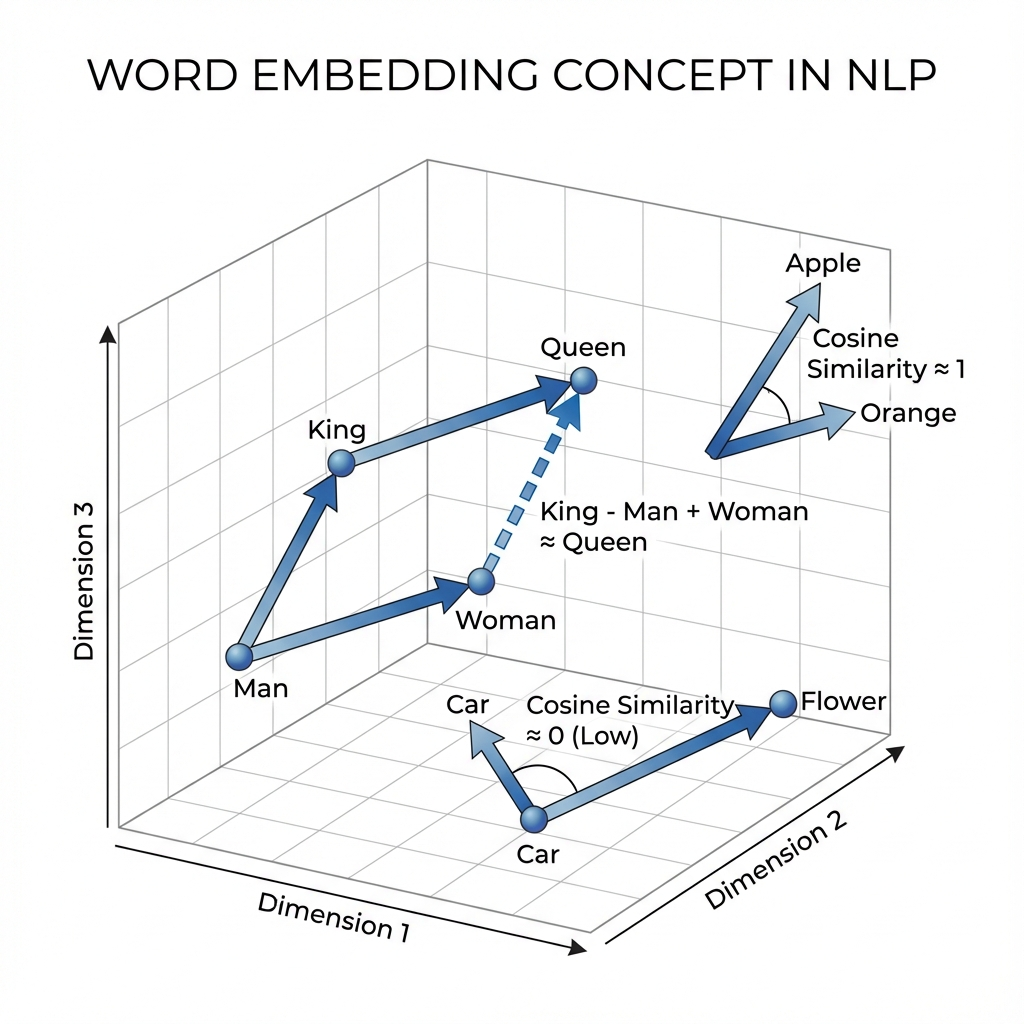
\includegraphics[width=0.7\textwidth]{Images/word_embedding.png}
    \caption{Minh họa không gian vector embedding và độ tương đồng cosine giữa các từ}
    \label{fig:word_embedding}
\end{figure}

Trong không gian embedding đa chiều (thường từ 512 đến 4096 chiều), các từ có ngữ nghĩa tương đồng sẽ có vector gần nhau. Độ tương đồng giữa hai vector thường được đo bằng cosine similarity:

\begin{equation}
\text{cosine\_similarity}(\mathbf{a}, \mathbf{b}) = \frac{\mathbf{a} \cdot \mathbf{b}}{\|\mathbf{a}\| \cdot \|\mathbf{b}\|} = \frac{\sum_{i=1}^{n} a_i b_i}{\sqrt{\sum_{i=1}^{n} a_i^2} \cdot \sqrt{\sum_{i=1}^{n} b_i^2}}
\end{equation}

Việc embedding giúp ``làm dày'' ngữ cảnh của mỗi data point, cho phép mô hình học được các mối quan hệ ngữ nghĩa phức tạp như:
\begin{itemize}
    \item $\text{vector}(\text{``King''}) - \text{vector}(\text{``Man''}) + \text{vector}(\text{``Woman''}) \approx \text{vector}(\text{``Queen''})$
    \item Các từ đồng nghĩa có vector gần nhau trong không gian embedding
    \item Các từ trong cùng ngữ cảnh có cosine similarity cao
\end{itemize}

\textbf{Cơ chế Self-Attention}

\begin{figure}[h!]
    \centering
    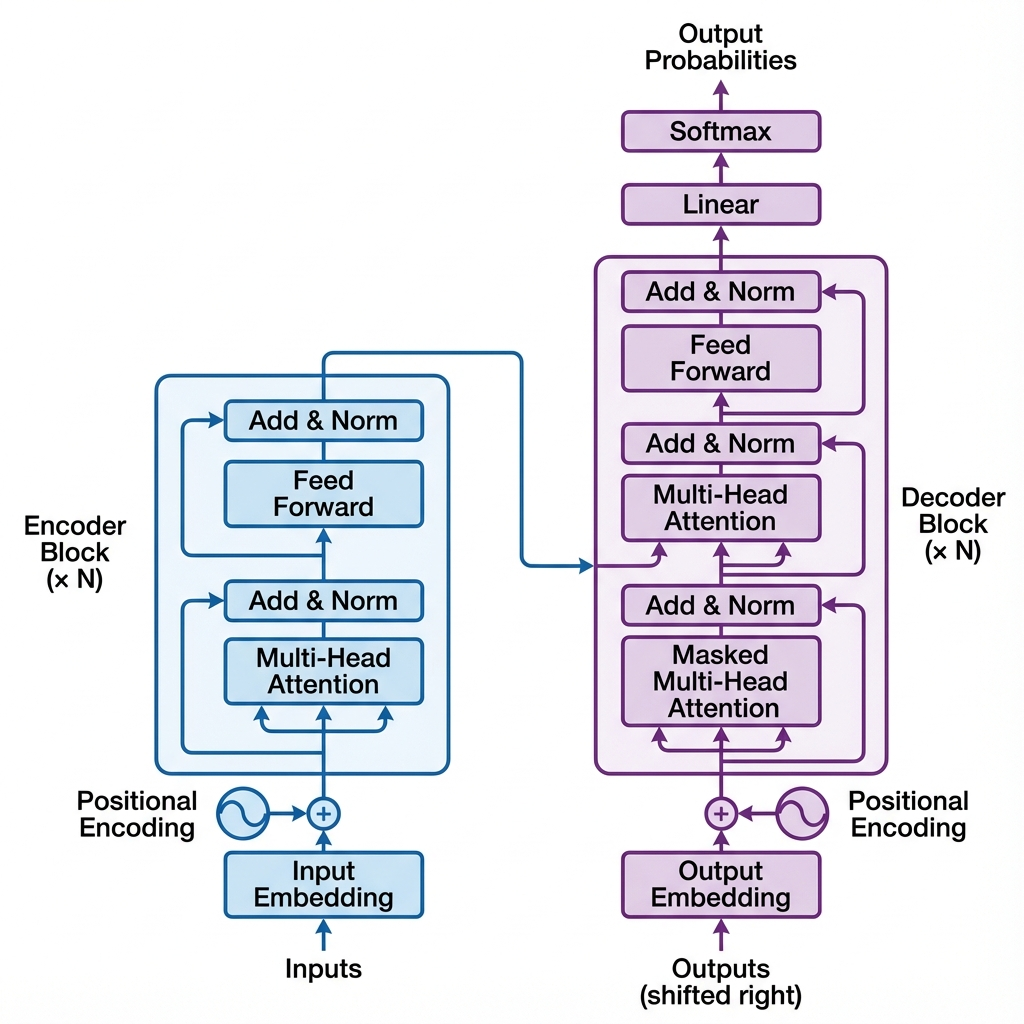
\includegraphics[width=0.8\textwidth]{Images/transformer_architecture.png}
    \vspace{6pt}
    \caption{Kiến trúc Transformer với các khối Encoder và Decoder}
    \label{fig:transformer_architecture}
\end{figure}
\begin{figure}[h!]
    \centering
    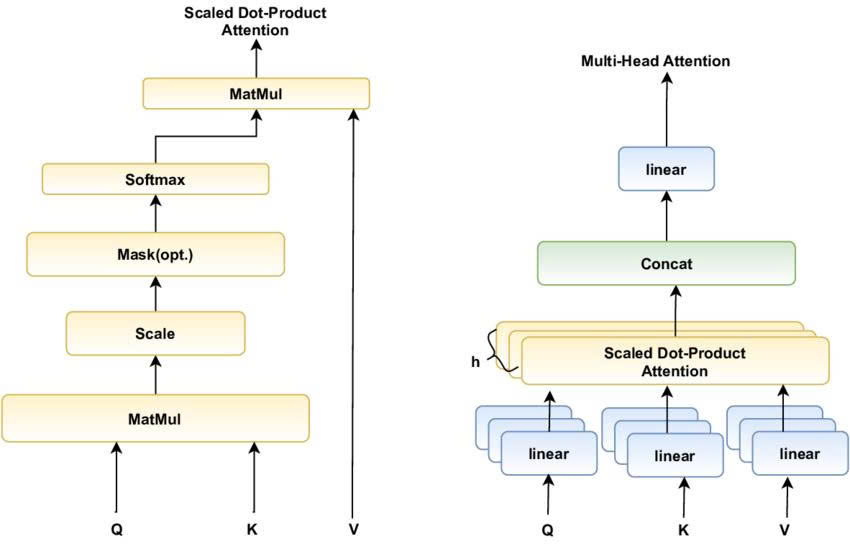
\includegraphics[width=0.85\textwidth]{Images/Self-Attention.jpg}
    \vspace{8pt}
    \caption{Cơ chế Self-Attention: Query, Key, Value và Scaled Dot-Product Attention}
    \label{fig:self_attention}
\end{figure}
Self-Attention cho phép mỗi vị trí trong chuỗi đầu vào ``chú ý'' đến tất cả các vị trí khác, học được mối quan hệ giữa các từ bất kể khoảng cách. Cơ chế này hoạt động thông qua ba ma trận: Query (Q), Key (K), và Value (V):

\begin{equation}
\text{Attention}(Q, K, V) = \text{softmax}\left(\frac{QK^T}{\sqrt{d_k}}\right)V
\end{equation}

Trong đó:
\begin{itemize}
    \item $Q$ (Query): Biểu diễn ``câu hỏi'' - token hiện tại muốn tìm thông tin gì
    \item $K$ (Key): Biểu diễn ``chìa khóa'' - các token khác chứa thông tin gì
    \item $V$ (Value): Biểu diễn ``giá trị'' - nội dung thực sự của các token
    \item $d_k$: Chiều của vector key, dùng để scale gradient ổn định
\end{itemize}

Multi-Head Attention mở rộng cơ chế này bằng cách chạy song song nhiều attention head, mỗi head học các loại quan hệ khác nhau:

\begin{equation}
\text{MultiHead}(Q, K, V) = \text{Concat}(\text{head}_1, ..., \text{head}_h)W^O
\end{equation}

Trong đó mỗi head được tính toán độc lập: $\text{head}_i = \text{Attention}(QW_i^Q, KW_i^K, VW_i^V)$

\textbf{Ưu điểm của Multi-Head Attention:}
\begin{itemize}
    \item \textbf{Đa dạng hóa biểu diễn}: Mỗi head có thể học các loại quan hệ khác nhau (ví dụ: head 1 học quan hệ cú pháp, head 2 học quan hệ ngữ nghĩa, head 3 học quan hệ vị trí).

    \item \textbf{Tối ưu hóa song song trên GPU}: Việc chia thành nhiều head độc lập cho phép tận dụng tối đa khả năng tính toán song song của GPU. Thay vì thực hiện một phép attention lớn với chiều $d_{model}$, ta thực hiện $h$ phép attention nhỏ với chiều $d_k = d_{model}/h$ song song. Điều này phù hợp hoàn hảo với kiến trúc SIMD (Single Instruction Multiple Data) của GPU, giúp:
    \begin{itemize}
        \item Tăng tốc độ training đáng kể nhờ batch matrix multiplication
        \item Tối ưu hóa throughput trong inference
        \item Sử dụng hiệu quả băng thông bộ nhớ GPU (memory bandwidth)
        \item Cho phép scale lên nhiều GPU dễ dàng hơn với tensor parallelism
    \end{itemize}

    \item \textbf{Giảm chi phí tính toán}: Tổng chi phí tính toán tương đương với single-head attention có cùng chiều $d_{model}$, nhưng hiệu quả hơn nhờ song song hóa.
\end{itemize}

\textbf{So sánh Transformer và CNN: Global Context vs Local Context}

Một trong những điểm mấu chốt của Transformer so với CNN là cách nắm bắt ngữ cảnh:

\begin{table}[h!]
\centering
\caption{So sánh Transformer và CNN}
\begin{tabular}{|l|p{6cm}|p{6cm}|}
\hline
\textbf{Đặc điểm} & \textbf{Transformer} & \textbf{CNN} \\
\hline
\textbf{Ngữ cảnh} & Global Context - Mỗi token có thể attention đến tất cả các token khác trong chuỗi & Local Context - Chỉ nhìn thấy các phần tử trong receptive field (kernel window) \\
\hline
\textbf{Inductive Bias} & Ít inductive bias $\rightarrow$ Cần lượng dữ liệu rất lớn để học & Có inductive bias mạnh về locality và translation equivariance \\
\hline
\textbf{Dữ liệu cần} & Yêu cầu dataset khổng lồ (hàng trăm GB văn bản) & Có thể hoạt động tốt với dataset nhỏ hơn \\
\hline
\textbf{Phức tạp} & $O(n^2)$ với độ dài chuỗi $n$ & $O(n \cdot k^2)$ với kernel size $k$ \\
\hline
\textbf{Ưu điểm} & Học được long-range dependencies tốt & Hiệu quả với dữ liệu có cấu trúc không gian (ảnh) \\
\hline
\end{tabular}
\end{table}

\textbf{Inductive Bias:} Transformer có rất ít giả định tiên nghiệm về cấu trúc dữ liệu (minimal inductive bias). Điều này có nghĩa là mô hình phải học toàn bộ ngữ cảnh và các pattern từ dữ liệu, thay vì có sẵn các ``bias'' như locality trong CNN. Hệ quả là Transformer cần lượng dữ liệu huấn luyện cực lớn để đạt được hiệu suất tốt.

\textbf{Kiến trúc Encoder-Decoder và Decoder-Only}

Transformer gốc bao gồm cả khối Encoder và Decoder:
\begin{itemize}
    \item \textbf{Encoder}: Xử lý chuỗi đầu vào, tạo biểu diễn ngữ cảnh. Sử dụng bidirectional attention (nhìn cả trái và phải).
    \item \textbf{Decoder}: Sinh chuỗi đầu ra từng token một, sử dụng cross-attention để tham chiếu đến encoder output.
\end{itemize}

Tuy nhiên, các mô hình sinh văn bản như GPT chỉ sử dụng \textbf{Decoder-Only} architecture với cơ chế \textbf{Masked Self-Attention} (hay Causal Attention):

\begin{equation}
\text{Masked-Attention}(Q, K, V) = \text{softmax}\left(\frac{QK^T}{\sqrt{d_k}} + M\right)V
\end{equation}

Trong đó $M$ là ma trận mask với $M_{ij} = -\infty$ nếu $j > i$ (các vị trí tương lai bị che). Điều này đảm bảo:
\begin{itemize}
    \item Mỗi token chỉ attend được đến các token trước nó (autoregressive)
    \item Tránh ``học vẹt'' (data leakage) - mô hình không thể nhìn thấy câu trả lời khi đang dự đoán
    \item Phù hợp cho các tác vụ sinh văn bản (text generation)
\end{itemize}

\textbf{Các Khối Phụ trợ trong Transformer}

\begin{itemize}
    \item \textbf{Layer Normalization}: Khác với Batch Normalization trong CNN, Layer Norm chuẩn hóa theo chiều feature thay vì theo batch. Điều này phù hợp hơn cho sequence data có độ dài thay đổi:
    \begin{equation}
    \text{LayerNorm}(x) = \gamma \cdot \frac{x - \mu}{\sqrt{\sigma^2 + \epsilon}} + \beta
    \end{equation}

    \item \textbf{Residual Connection}: Skip connection giúp gradient flow tốt hơn và cho phép đào tạo các mạng rất sâu.

    \item \textbf{Feed-Forward Network (FFN)}: Mỗi layer có một FFN với hidden dimension lớn (thường 4x embedding dimension):
    \begin{equation}
    \text{FFN}(x) = \max(0, xW_1 + b_1)W_2 + b_2
    \end{equation}

    \item \textbf{Positional Encoding}: Vì Transformer không có khái niệm về thứ tự, positional encoding được thêm vào để mã hóa vị trí của các token trong chuỗi.
\end{itemize}

\textbf{b) Các mô hình LLM tiêu biểu và các bước ngoặt}

Sự phát triển của LLM đã trải qua nhiều bước ngoặt quan trọng:

\textbf{Các bước ngoặt trong lịch sử LLM:}
\begin{enumerate}
    \item \textbf{GPT-1 (2018)}: OpenAI giới thiệu khái niệm pre-training + fine-tuning, chứng minh unsupervised pre-training có thể cải thiện NLP tasks.

    \item \textbf{BERT (2018)}: Google đề xuất bidirectional pre-training với masked language modeling, tạo bước đột phá trong NLU (Natural Language Understanding).

    \item \textbf{GPT-3 (2020)}: Với 175 tỷ tham số, GPT-3 chứng minh khả năng few-shot learning mà không cần fine-tuning, mở ra kỷ nguyên prompt engineering.

    \item \textbf{ChatGPT (2022)}: Sử dụng RLHF (Reinforcement Learning from Human Feedback) để align với mong muốn người dùng, tạo AI conversational thực sự hữu ích.

    \item \textbf{GPT-4 (2023)}: Mô hình đa phương thức (multimodal) có thể xử lý cả văn bản và hình ảnh, reasoning ability được cải thiện đáng kể.

    \item \textbf{Open-source revolution (2023-2024)}: LLaMA (Meta), Mistral, Qwen mở cửa cho cộng đồng nghiên cứu và triển khai local.

    \item \textbf{DeepSeek (2024)}: Bước ngoặt quan trọng từ Trung Quốc, DeepSeek-V3 đạt hiệu suất cạnh tranh với GPT-4 với chi phí huấn luyện thấp hơn đáng kể (chỉ \$5.6M), chứng minh hiệu quả của kiến trúc Mixture of Experts (MoE) và kỹ thuật Multi-head Latent Attention (MLA).
\end{enumerate}

\textbf{Bảng so sánh các mô hình LLM tiêu biểu:}

\begin{table}[h!]
\centering
\resizebox{\textwidth}{!}{
\begin{tabular}{|l|c|c|c|c|c|}
\hline
\textbf{Mô hình} & \textbf{Nhà phát triển} & \textbf{Tham số} & \textbf{Open-source} & \textbf{Đa phương thức} & \textbf{Đặc điểm nổi bật} \\
\hline
GPT-4o & OpenAI & N/A & Không & Có & SOTA reasoning, API phổ biến \\
\hline
Gemini 2.0 & Google & N/A & Không & Có & Tích hợp Google Search, dài context \\
\hline
Claude 3.5 & Anthropic & N/A & Không & Có & An toàn, coding mạnh \\
\hline
LLaMA 3.1 & Meta & 8B-405B & Có & Hạn chế & Cộng đồng lớn, dễ fine-tune \\
\hline
Mistral Large & Mistral AI & 7B-123B & Có & Có & Nhẹ, hiệu quả cho edge \\
\hline
Qwen 2.5 & Alibaba & 0.5B-72B & Có & Có & Đa ngôn ngữ, nhiều size \\
\hline
DeepSeek-V3 & DeepSeek & 671B MoE & Có & Có & Chi phí thấp, MoE hiệu quả \\
\hline
\end{tabular}
}
\label{tab:llm_comparison}
\end{table}

\textbf{Xu hướng hiện tại trong LLM:}
\begin{itemize}
    \item \textbf{Mixture of Experts (MoE)}: Chỉ kích hoạt một phần nhỏ tham số mỗi lần, giảm chi phí inference (DeepSeek, Mixtral).
    \item \textbf{Long context}: Mở rộng context window lên 128K-2M tokens (Gemini, Claude).
    \item \textbf{Multimodal}: Xử lý văn bản, hình ảnh, âm thanh, video trong cùng một mô hình.
    \item \textbf{Edge deployment}: Các mô hình nhỏ (1B-7B) chạy được trên smartphone và thiết bị nhúng.
    \item \textbf{Reasoning}: Cải thiện khả năng suy luận logic và toán học (o1, DeepSeek-R1).
\end{itemize}


\textbf{c) Kỹ thuật Prompt Engineering}

Prompt engineering là nghệ thuật thiết kế câu lệnh (prompt) để điều khiển hành vi của LLM. Các kỹ thuật prompting chính được so sánh trong bảng sau:

\begin{table}[h!]
\centering
\resizebox{\textwidth}{!}{
\begin{tabular}{|l|p{4cm}|p{5cm}|p{3cm}|}
\hline
\textbf{Kỹ thuật} & \textbf{Mô tả} & \textbf{Ví dụ prompt} & \textbf{Phù hợp với} \\
\hline
Zero-shot & Yêu cầu trực tiếp không có ví dụ & ``Dịch sang tiếng Anh: Xin chào'' & Tác vụ đơn giản \\
\hline
Few-shot & Cung cấp 2-5 ví dụ mẫu trước khi hỏi & ``Ví dụ: Mèo $\rightarrow$ Cat. Chó $\rightarrow$ Dog. Nhà $\rightarrow$ ?'' & Tác vụ cần định dạng cụ thể \\
\hline
System Prompt & Định nghĩa vai trò và quy tắc cho agent & ``Bạn là trợ lý y tế, luôn khuyên bệnh nhân gặp bác sĩ'' & Chatbot, AI Agent \\
\hline
\end{tabular}
}
\label{tab:prompting_techniques}
\end{table}

%=========================================

\subsubsection{Hệ thống chuyển đổi Giọng nói (STT \& TTS)}

Để tạo ra một vòng lặp giao tiếp tự nhiên hoàn chỉnh giữa người và máy (Human-Computer Interaction), hệ thống không chỉ xử lý văn bản mà còn phải nghe và nói. Điều này được thực hiện qua hai quy trình:

\begin{itemize}
    \item \textbf{Speech-to-Text (STT - Chuyển đổi Giọng nói thành Văn bản)}: Thu nhận sóng âm (audio waveform) từ microphone của robot, lọc nhiễu, phân tích phổ âm (spectrogram) và sử dụng các mô hình học sâu âm học để nhận diện và chuyển đổi thành chuỗi văn bản. Trong hệ thống này, văn bản thu được từ STT sẽ đóng vai trò làm câu lệnh (prompt) đầu vào cho LLM thông qua Groq API.
    \item \textbf{Text-to-Speech (TTS - Chuyển đổi Văn bản thành Giọng nói)}: Nhận chuỗi văn bản đầu ra từ LLM và tổng hợp thành tín hiệu âm thanh giọng nói con người. Hệ thống TTS hiện đại tạo ra giọng nói rất tự nhiên, có ngữ điệu và cảm xúc, giúp robot trở nên thân thiện hơn khi trò chuyện, nhắc nhở uống thuốc hoặc cảnh báo nguy hiểm.
\end{itemize}

Sự kết hợp giữa STT, Groq API (LLM siêu tốc) và TTS tạo nên một "bộ não" giao tiếp bằng giọng nói liên tục, đóng vai trò như một người bạn đồng hành ảo, hỗ trợ tương tác tự nhiên tối đa cho người cao tuổi vốn không quen thao tác trên màn hình cảm ứng.


% --- Tích hợp từ phần cũ ---
\subsubsection{Một số giải pháp Nhận dạng Giọng nói:}

Dưới đây là bảng so sánh các giải pháp chuyển đổi giọng nói thành văn bản (Speech-to-Text) phổ biến hiện nay:

\begin{table}[htbp]
\centering
\small
\begin{tabularx}{\textwidth}{@{} l >{\raggedright\arraybackslash}X >{\raggedright\arraybackslash}X >{\raggedright\arraybackslash}X @{}}
\toprule
\textbf{Tiêu chí} & \textbf{Google Speech-to-Text} & \textbf{OpenAI Whisper} & \textbf{Vosk} \\ \midrule
\textbf{Hình thức} & Cloud API (SaaS) & Open-source (Local/Cloud) & Open-source (Local) \\
\textbf{Độ chính xác} & Rất cao (đặc biệt tiếng Việt) & Cực cao (State-of-the-art) & Khá (tùy thuộc model) \\
\textbf{Internet} & Bắt buộc & Không bắt buộc & Không cần thiết \\
\textbf{Tốc độ} & Phụ thuộc băng thông & Phụ thuộc GPU/CPU & Rất nhanh (Real-time) \\
\textbf{Chi phí} & Trả phí theo lưu lượng & Miễn phí phần mềm & Miễn phí \\
\textbf{Phù hợp} & Ứng dụng mobile cần độ chính xác tối đa. & Robot có phần cứng mạnh, cần hiểu ngữ cảnh sâu. & Thiết bị nhúng (Raspberry Pi), phản hồi cực nhanh. \\ \bottomrule
\end{tabularx}
\caption{So sánh các công nghệ Speech-to-Text.}
\end{table}

\subsubsection{Phương pháp tiếp cận Xử lý Ngôn ngữ Tự nhiên (NLP) trong dự án}

Thay vì tự phát triển các mô hình NLP cục bộ (như Rule-based hay phân loại Intent bằng Machine Learning) vốn bị hạn chế về khả năng hiểu ngữ cảnh tự nhiên, hoặc triển khai trực tiếp các mô hình Deep Learning lớn gây quá tải cho phần cứng robot (edge devices), đồ án tiếp cận theo hướng hoàn toàn dựa vào API.

Cụ thể, hệ thống không huấn luyện hay lưu trữ mô hình ngôn ngữ riêng mà gọi trực tiếp \textbf{Groq API} để xử lý văn bản (sau khi âm thanh được STT dịch ra). Để duy trì tính mạch lạc trong giao tiếp (contextual memory), hệ thống không sử dụng các giải pháp lưu trữ phức tạp hay RAG, mà đơn giản sử dụng cơ chế \textbf{Session Chat} (Lưu trữ phiên trò chuyện). Trong cơ chế này, lịch sử của một vài vòng thoại gần nhất được lưu tạm thời trên RAM của ứng dụng và đính kèm vào phần \textit{prompt} gửi đi mỗi lần. Nhờ vậy, LLM có thể "nhớ" được ngữ cảnh trò chuyện ngắn hạn, giúp phản hồi tự nhiên hơn với chi phí lập trình và tài nguyên hệ thống thấp nhất.


\subsubsection{Phương thức triển khai: Điện toán Biên (Edge Computing) trên thiết bị Android}
Để đảm bảo hệ thống phản hồi theo thời gian thực, bảo vệ quyền riêng tư và tối ưu hóa băng thông mạng, đồ án đặt trọng tâm vào phương thức triển khai \textbf{Edge Computing} (Điện toán biên) trực tiếp trên thiết bị Android (Smartphone).

Toàn bộ các luồng xử lý cốt lõi bao gồm: thu nhận hình ảnh từ camera, chạy mô hình phát hiện đối tượng (YOLO26), theo dõi đa đối tượng (ByteTrack), và phân tích chuỗi thời gian bằng mạng LSTM để phát hiện té ngã, đều được thực thi hoàn toàn ở thiết bị biên thông qua bộ tăng tốc phần cứng (NPU/GPU trên điện thoại) kết hợp với các runtime như TensorFlow Lite.

Việc triển khai Edge Computing mang lại các ưu điểm vượt trội:
\begin{itemize}
    \item \textbf{Độ trễ thấp (Low Latency):} Xử lý ảnh tại chỗ giúp robot phát hiện người ngã ngay lập tức mà không phải chờ dữ liệu gửi lên và tải về từ server.
    \item \textbf{Đảm bảo quyền riêng tư (Privacy):} Dữ liệu hình ảnh sinh hoạt riêng tư của người cao tuổi không bị truyền ra ngoài môi trường Internet.
    \item \textbf{Độ tin cậy cao:} Hệ thống vẫn hoạt động ổn định các tính năng cốt lõi ngay cả khi mất kết nối mạng.
\end{itemize}
Riêng với tính năng giao tiếp hội thoại (NLP/Chat), thiết bị mới đóng vai trò làm client gọi Groq API (như đã trình bày) nhằm tận dụng năng lực suy luận ngôn ngữ, trong khi toàn bộ phần nhận thức thị giác máy tính và phân tích hành vi đều vận hành độc lập theo mô hình Edge Computing thuần túy.







\subsection{Giới thiệu Dataset Fall Detection – LE2I}
%=========================================

\subsubsection{Mục tiêu và đặc điểm của dataset LE2I}

LE2I Fall Detection Dataset là một trong những bộ dữ liệu chuẩn mực và phổ biến nhất dành cho bài toán phát hiện té ngã, được phát triển bởi phòng thí nghiệm Le2i (Đại học Burgundy, Pháp). Bộ dữ liệu cung cấp các video mô phỏng các hoạt động thường ngày (Activities of Daily Living - ADL) và các tình huống té ngã đa dạng \reportcite{ref:le2i}.

Đặc điểm nổi bật của dataset LE2I:
\begin{itemize}
    \item \textbf{Môi trường thực tế}: Được quay ở 4 bối cảnh khác nhau bao gồm: Nhà ở (Home), Phòng cafe (Coffee room), Văn phòng (Office) và Phòng học (Lecture room).
    \item \textbf{Đa dạng kịch bản ngã}: Bao gồm ngã về phía trước, phía sau, ngã do mất thăng bằng, hoặc ngã khi đang cố gắng đứng lên.
    \item \textbf{Nhiễu tự nhiên}: Video chứa các thách thức thực tế như đổ bóng (shadows), thay đổi ánh sáng (illumination variations), và che khuất (occlusions) do đồ vật.
\end{itemize}

\subsubsection{Dữ liệu video và Annotation}

Dataset LE2I bao gồm khoảng 191 video với các đặc điểm:
\begin{figure}[h!]
    \centering
    \includegraphics[width=0.85\textwidth]{Images/1.jpeg}
    \caption{Một số khung hình minh họa trong môi trường của dataset LE2I.}
\end{figure}
\begin{itemize}
    \item Độ phân giải video là 320x240 pixels với tốc độ khung hình 25 FPS.
    \item Annotation cung cấp khung hình bắt đầu và kết thúc quá trình ngã (ground truth frame numbers), kết hợp với thông tin Bounding Box của người.
    \item Các nhãn cơ bản gồm trạng thái ngã (fall) và hoạt động bình thường (no\_fall).
\end{itemize}

\subsubsection{Ưu điểm và hạn chế của dataset LE2I}

\textbf{Ưu điểm:}
\begin{itemize}
    \item Bối cảnh phong phú, từ không gian chật hẹp (văn phòng) đến rộng rãi (phòng học).
    \item Các tình huống ngã được diễn viên thực hiện tự nhiên, bao gồm các hoạt động khó phân biệt như cúi nhặt đồ hoặc ngồi xuống nhanh.
    \item Là chuẩn đối sánh (benchmark) uy tín được sử dụng rộng rãi trong các nghiên cứu Fall Detection.
\end{itemize}

\textbf{Hạn chế:}
\begin{itemize}
    \item Độ phân giải video tương đối thấp (320x240) so với các chuẩn camera HD hiện đại.
    \item Số lượng chủ thể (diễn viên) còn hạn chế so với các dataset quy mô lớn gần đây.
\end{itemize}

\subsubsection{So sánh với các Dataset quy mô lớn (DiverseFALL10500)}

Gần đây, một số nghiên cứu đề xuất các bộ dữ liệu khổng lồ như DiverseFALL10500 (10,500 ảnh) để khắc phục nhược điểm của các dataset cũ \reportcite{ref:falldetection}.

\textbf{So sánh LE2I và DiverseFALL10500:}
\begin{center}
\begin{tabular}{|l|c|c|}
\hline
\textbf{Tiêu chí} & \textbf{LE2I Dataset} & \textbf{DiverseFALL10500} \\
\hline
Số lượng video/ảnh & 191 videos & 10,500 images \\
Môi trường & 4 môi trường trong nhà & Indoor + Outdoor \\
Độ phân giải & 320x240 & Đa dạng (HD) \\
Yếu tố che khuất & Tích hợp sẵn (bàn, ghế) & Đa dạng \\
\hline
\end{tabular}
\end{center}

Đồ án này lựa chọn sử dụng (hoặc kết hợp) LE2I do đặc thù bộ dữ liệu này phản ánh rất sát các kịch bản trong môi trường nhà ở và có chứa chuỗi chuyển động thời gian (video), vô cùng phù hợp để trích xuất Tracklet cho mô hình LSTM.

%=========================================
\subsection{Suy luận AI trên thiết bị và TensorFlow Lite}

Edge AI xử lý dữ liệu gần nguồn thay vì gửi toàn bộ lên cloud. Với camera trong nhà, cách này giảm lưu lượng, độ trễ và phạm vi truyền ảnh; đồng thời vẫn cần kiểm soát quyền và lưu trữ cục bộ. TensorFlow Lite cung cấp runtime cho thiết bị di động/biên, hỗ trợ interpreter CPU và delegate phần cứng \reportcite{ref:tflite}.

Chuỗi chuyển đổi thường gồm model huấn luyện $\rightarrow$ biểu diễn trung gian $\rightarrow$ TFLite. Ba vấn đề phải kiểm chứng là: shape/layout tensor; toán tử được runtime/delegate hỗ trợ; và sai số số học sau tối ưu. FP16 giảm kích thước trọng số và băng thông bộ nhớ, nhưng không bảo đảm tăng tốc nếu delegate không sử dụng FP16. INT8 có thể giảm sâu hơn nhưng cần representative dataset và kiểm tra suy giảm keypoint/metric.

NMS có thể đặt trong graph hoặc ngoài graph. NMS trong graph giảm code hậu xử lý nhưng dễ tạo toán tử không tương thích delegate. NMS ngoài graph yêu cầu decoder Kotlin chính xác, đổi lại graph gọn và dễ chạy GPU hơn. Vì vậy kết quả chuyển đổi cần so ở cả tensor và detection cuối cùng.

\subsection{Firebase Authentication và Realtime Database}

Realtime Database tổ chức dữ liệu thành cây JSON và đồng bộ thay đổi tới client đang lắng nghe \reportcite{ref:firebase_rtdb}. Client Android có cache và hàng đợi write, do đó callback ``gần thời gian thực'' không đồng nghĩa bản ghi luôn mới. Đối với lệnh robot, timestamp/expiry là phần của ngữ nghĩa dữ liệu, không chỉ là metadata.

Firebase Authentication cung cấp UID cho người dùng; Security Rules chạy phía máy chủ quyết định read/write và có thể validate kiểu/cấu trúc \reportcite{ref:firebase_security}. Rules mặc định cần từ chối, sau đó cấp quyền tối thiểu theo UID, family và robot. Các node lệnh/signaling không nên dùng chung toàn cục trong hệ thống nhiều robot. Chúng cũng cần validate miền giá trị, người gửi và vòng đời phiên.

Ưu điểm của RTDB là tích hợp Android nhanh, listener đơn giản và phù hợp state/event nhỏ. Hạn chế là schema phi quan hệ, truy vấn có giới hạn và dễ tạo coupling bằng string path. Tách repository/data access, định nghĩa model chung và test rules bằng emulator giúp giảm rủi ro.

\subsection{WebRTC, signaling và ICE}

WebRTC là tập API/giao thức cho media và dữ liệu thời gian thực giữa các peer \reportcite{ref:webrtc}. Một phiên cần signaling để trao đổi Session Description Protocol (SDP) và ICE candidate, nhưng chuẩn không bắt buộc một công nghệ signaling cụ thể. Đề tài dùng RTDB cho phần này.

ICE thu thập candidate và kiểm tra cặp đường truyền để vượt Network Address Translator \reportcite{ref:ice}. STUN giúp peer biết địa chỉ public; TURN relay media khi không tạo được đường trực tiếp. Do đó có TURN làm tăng tỷ lệ kết nối nhưng thêm băng thông/độ trễ/chi phí máy chủ. Trạng thái call ở database và trạng thái PeerConnection là hai state machine khác nhau, cần cleanup idempotent để tránh phiên cũ.

WebRTC mã hóa media theo kiến trúc bảo mật giao thức, nhưng ứng dụng vẫn phải bảo vệ signaling, quyền camera/micro và danh tính peer \reportcite{ref:webrtc_security}. SDP/ICE có thể lộ thông tin mạng; log không nên lưu vô hạn. Trong hệ thống chăm sóc, phải có chỉ báo rõ khi camera/micro đang truyền.

\subsection{Bluetooth Low Energy và GATT}

BLE phù hợp liên kết cự ly gần giữa điện thoại và vi điều khiển. GATT xây trên bảng attribute, tổ chức dữ liệu thành service, characteristic và descriptor \reportcite{ref:ble_primer}. Server công bố service/characteristic; client quét, kết nối, khám phá và thực hiện read/write/notify theo property.

Write without response giảm round-trip và phù hợp dòng lệnh cập nhật thường xuyên, nhưng không có ACK ở tầng GATT cho từng write. Ứng dụng phải dùng gửi lặp, sequence/timestamp và watchdog. UUID 128-bit cho custom service tránh xung đột profile chuẩn. Payload văn bản dễ debug nhưng tốn byte và parser cần chặt; protocol nhị phân với version, sequence và checksum là hướng nâng cấp.

BLE disconnect là trạng thái bình thường có thể xảy ra do khoảng cách, radio hoặc vòng đời Android. Motor vì vậy không được giữ setpoint cuối. Callback disconnect và timeout độc lập ở firmware là yêu cầu an toàn, không nên chỉ dựa vào app.

\subsection{Động cơ BLDC và điều khiển FOC}

Động cơ BLDC/PMSM tạo mô-men bằng tương tác từ trường stator và rotor nam châm. Field-Oriented Control biến đổi dòng ba pha sang hệ trục quay $d$--$q$, tách thành phần từ thông và mô-men, sau đó dùng PWM để điều khiển điện áp \reportcite{ref:foc}. Với encoder từ AS5600, hệ thống có phản hồi góc/tốc độ cho vòng kín.

Vòng điều khiển vận tốc so sánh tốc độ đặt với tốc độ đo. PID có dạng khái quát:

\begin{equation}
u(t)=K_pe(t)+K_i\int_0^t e(\tau)d\tau+K_d\frac{de(t)}{dt}.
\end{equation}

Giới hạn điện áp bảo vệ driver/motor; giới hạn vận tốc bảo vệ cơ khí; lọc thông thấp giảm nhiễu đo. Deadzone giúp thắng ma sát tĩnh nhưng có thể tạo bước nhảy tốc độ, vì vậy bản hoàn thiện nên bổ sung ramp/giới hạn gia tốc. SimpleFOC cung cấp các abstraction motor, driver, sensor và vòng \texttt{loopFOC}/\texttt{move} cho vi điều khiển \reportcite{ref:simplefoc}.

\subsection{An toàn và quản trị rủi ro AI}

Một hệ thống cảnh báo người cao tuổi phải xem cả false positive và false negative. False positive lặp lại làm người dùng mất tin cậy; false negative có thể trì hoãn hỗ trợ. NIST AI RMF đề xuất các chức năng govern, map, measure và manage xuyên suốt vòng đời \reportcite{ref:nist_ai_rmf}. Với đồ án, điều này được cụ thể hóa bằng phạm vi sử dụng rõ, metric theo sự cố, log bằng chứng, giám sát lỗi, fallback và công bố giới hạn.

LLM không nên là thành phần duy nhất quyết định an toàn. Từ khóa cục bộ xử lý câu rõ, LLM chỉ phân loại trường hợp mơ hồ và lỗi mặc định nguy hiểm. Tương tự, output LSTM đi qua state machine/hậu kiểm. Các lớp độc lập làm hệ thống dễ kiểm tra hơn, nhưng không thay thế đánh giá thực địa.

\subsection{Kết luận chương}
%=========================================

Chương đã trình bày nền tảng robot dựa trên smartphone, mạng nơ-ron, CNN, detector họ YOLO, pose, dữ liệu té ngã, tracking, LSTM, LLM, nhận dạng giọng nói, AI biên, Firebase, WebRTC, BLE và FOC. Các nội dung được liên kết với lựa chọn hiện thực thay vì giả định một mô hình khảo sát chính là model cuối. Điểm then chốt là phát hiện té ngã của đề tài không dựa trên một nhãn ảnh duy nhất mà kết hợp pose, duy trì ID0, chuỗi LSTM và hậu kiểm có bằng chứng. Chương tiếp theo chuyển các khái niệm này thành yêu cầu, kiến trúc và hợp đồng cụ thể.

\clearpage
\section{Phân tích và thiết kế hệ thống}

Chương này trình bày quá trình phân tích yêu cầu và thiết kế hệ thống robot trợ lý hỗ trợ chăm sóc người cao tuổi tại nhà. Từ mục tiêu giao tiếp, nhắc nhở, giám sát, cảnh báo té ngã và hỗ trợ can thiệp từ xa, các yêu cầu chức năng và yêu cầu chất lượng được xác định làm cơ sở xây dựng kiến trúc cùng các luồng xử lý. Kiến trúc vận hành gồm ứng dụng trên robot, ứng dụng của người chăm sóc, dịch vụ dùng chung và phần thân robot. Quy trình chuẩn bị mô hình AI được xem xét riêng để cung cấp mô hình cho ứng dụng trên robot. Chương cũng phân tích các phương án công nghệ, giao thức truyền thông và cơ chế an toàn làm cơ sở cho quá trình hiện thực ở Chương 4.

\subsection{Phân tích yêu cầu hệ thống}

\subsubsection{Bài toán, mục tiêu và phạm vi}

Đề tài hướng đến xây dựng một robot di động hoạt động trong môi trường trong nhà, sử dụng điện thoại hoặc máy tính bảng gắn trên robot làm bộ xử lý chính. Hệ thống hỗ trợ người cao tuổi thông qua hội thoại bằng giọng nói, nhắc nhở theo lịch, giám sát bằng thị giác, phát hiện tình huống nghi té ngã và liên lạc với người chăm sóc. Một ứng dụng riêng dành cho người chăm sóc cung cấp khả năng quản lý thông tin, theo dõi sự kiện và can thiệp từ xa. Phần thân robot tiếp nhận lệnh chuyển động từ thiết bị gắn trên robot và điều khiển hai bánh xe theo yêu cầu.

Các định hướng của luận văn được cụ thể hóa trong Bảng \ref{tab:thesis_requirement_refinement}. Trong phạm vi đề tài, khả năng hiểu ngôn ngữ tự nhiên tập trung vào hội thoại hằng ngày, nhận biết yêu cầu liên lạc với người chăm sóc và diễn giải câu trả lời khi xác nhận tình trạng sau một sự kiện nghi té ngã. Hệ thống chỉ đóng vai trò hỗ trợ chăm sóc, giám sát và liên lạc; không phải thiết bị chẩn đoán y khoa, không thay thế người chăm sóc và không tự đưa ra quyết định điều trị.

\begin{longtable}{|p{4.0cm}|p{5.0cm}|p{4.5cm}|}
\caption{Cụ thể hóa yêu cầu luận văn theo phạm vi đề tài}\label{tab:thesis_requirement_refinement}\\
\hline
\textbf{Định hướng ban đầu} & \textbf{Mục tiêu cụ thể} & \textbf{Kết quả cần đạt} \\
\hline
\endfirsthead
\hline
\textbf{Định hướng ban đầu} & \textbf{Mục tiêu cụ thể} & \textbf{Kết quả cần đạt} \\
\hline
\endhead
Tìm hiểu Intel OpenBot và giao tiếp điện thoại--robot & Khảo sát mô hình sử dụng điện thoại thông minh làm bộ xử lý và giao tiếp với phần thân robot & Xây dựng được phương thức kết nối để truyền lệnh chuyển động từ điện thoại đến thân robot \\
\hline
Nhận dạng giọng nói và hiểu ngôn ngữ tự nhiên & Xây dựng khả năng tiếp nhận tiếng nói, diễn giải nội dung và phản hồi bằng giọng nói & Hỗ trợ hội thoại hằng ngày, yêu cầu liên lạc và xác nhận tình trạng của người dùng \\
\hline
AI và IoT cho xử lý, điều khiển và tích hợp & Kết hợp xử lý thông minh trên robot với khả năng trao đổi dữ liệu và điều khiển giữa các thành phần & Đồng bộ được thông tin chăm sóc, trạng thái giám sát, sự kiện và lệnh điều khiển \\
\hline
Thị giác máy tính cho giám sát và theo dõi & Nhận biết người, theo dõi người mục tiêu và phân tích sự thay đổi tư thế theo thời gian & Hỗ trợ robot bám theo người và phát hiện tình huống nghi té ngã \\
\hline
Đánh giá thuật toán và hệ thống kết nối & Đánh giá chất lượng nhận biết, tốc độ xử lý và khả năng trao đổi dữ liệu giữa các thành phần & Xác định được mức đáp ứng của nguyên mẫu, các giới hạn và hướng cải tiến \\
\hline
\end{longtable}

Phạm vi của đề tài gồm quản lý hồ sơ và lịch nhắc nhở; hội thoại bằng giọng nói; ước lượng tư thế, theo dõi một người mục tiêu, tự động bám theo và phát hiện té ngã; gọi video hai chiều; điều khiển robot bằng cần điều khiển ảo; ghi nhật ký nhắc nhở, cảnh báo và cuộc gọi. Các chức năng định vị và lập bản đồ toàn bộ ngôi nhà, tránh vật cản bằng cảm biến chuyên dụng, đo chỉ số sinh tồn, đánh giá bảo mật chuyên sâu và triển khai hệ thống ở quy mô lớn trong môi trường thực tế chưa được xem xét trong phạm vi này.

\subsubsection{Tác nhân, điều kiện vận hành và ranh giới hệ thống}

Hai tác nhân chính của hệ thống là người cao tuổi và người chăm sóc. Người cao tuổi tương tác trực tiếp với robot để nhận hỗ trợ, trong khi người chăm sóc quản lý thông tin và can thiệp từ xa. Bên trong ranh giới hệ thống gồm ứng dụng trên robot, ứng dụng của người chăm sóc, khối xử lý AI và phần thân robot. Các dịch vụ trực tuyến nằm ngoài ranh giới này nhưng cung cấp khả năng xác thực, đồng bộ dữ liệu, xử lý ngôn ngữ và hỗ trợ thiết lập liên lạc.

\begin{table}[H]
\centering
\caption{Tác nhân và các thành phần hỗ trợ của hệ thống}
\label{tab:actors}
\small
\begin{tabularx}{\textwidth}{|p{3.0cm}|X|X|}
\hline
\textbf{Đối tượng} & \textbf{Vai trò} & \textbf{Tương tác với hệ thống} \\
\hline
Người cao tuổi & Người sử dụng được hỗ trợ & Trò chuyện với robot, nhận lời nhắc, được giám sát trong phạm vi cho phép và tham gia cuộc gọi \\
\hline
Người chăm sóc & Người quản lý và hỗ trợ từ xa & Quản lý hồ sơ và lịch nhắc nhở, cấu hình chức năng, xem nhật ký, thực hiện cuộc gọi và điều khiển robot khi cần \\
\hline
Dịch vụ trực tuyến & Thành phần hỗ trợ bên ngoài & Cung cấp xác thực, đồng bộ dữ liệu, xử lý hội thoại và hỗ trợ thiết lập liên lạc từ xa \\
\hline
Phần thân robot & Thành phần chấp hành & Tiếp nhận lệnh chuyển động, điều khiển hai bánh xe và dừng khi mất lệnh \\
\hline
\end{tabularx}
\end{table}

Hệ thống giả định thiết bị gắn trên robot có camera, microphone, loa và khả năng kết nối không dây với phần thân robot. Thiết bị trên robot và thiết bị của người chăm sóc cần có kết nối Internet đối với các chức năng sử dụng dịch vụ trực tuyến. Các chức năng xử lý hình ảnh tại chỗ vẫn có thể tiếp tục khi mạng tạm thời gián đoạn, trong khi hội thoại trực tuyến, đồng bộ từ xa và thiết lập cuộc gọi phụ thuộc vào kết nối mạng.

\subsubsection{Yêu cầu chức năng}

Trên cơ sở mục tiêu, phạm vi và các tác nhân đã xác định, hệ thống cần cung cấp một nhóm chức năng xuyên suốt từ hỗ trợ người cao tuổi đến giám sát và điều khiển robot. Các yêu cầu này được tổng hợp trong Bảng \ref{tab:functional_requirements}; mỗi yêu cầu được gán một mã riêng để thuận tiện liên kết với các khối thiết kế và đối chiếu với kết quả kiểm thử ở những phần tiếp theo.

\begin{longtable}{|p{1.2cm}|p{4.0cm}|p{8.1cm}|}
\caption{Danh sách yêu cầu chức năng}\label{tab:functional_requirements}\\
\hline
\textbf{Mã} & \textbf{Yêu cầu} & \textbf{Mô tả chức năng} \\
\hline
\endfirsthead
\hline
\textbf{Mã} & \textbf{Yêu cầu} & \textbf{Mô tả chức năng} \\
\hline
\endhead
FR01 & Xác thực và liên kết người dùng & Hệ thống cho phép đăng ký, đăng nhập và xác định đúng không gian dữ liệu dùng chung giữa robot với người chăm sóc. \\
\hline
FR02 & Quản lý hồ sơ chăm sóc & Người chăm sóc có thể xem và cập nhật thông tin nhận diện, cách xưng hô, thông tin liên hệ, tình trạng, ghi chú và sở thích của người được chăm sóc. \\
\hline
FR03 & Quản lý lịch nhắc nhở & Người chăm sóc có thể tạo, chỉnh sửa, bật, tắt và xóa lịch nhắc nhở theo các chế độ một lần, hằng ngày, hằng tuần hoặc hằng tháng. \\
\hline
FR04 & Thực hiện và ghi nhận lời nhắc & Khi đến thời điểm đã thiết lập, robot phát lời nhắc, tiếp nhận phản hồi của người cao tuổi và lưu lại kết quả thực hiện. \\
\hline
FR05 & Hội thoại bằng giọng nói & Hệ thống tiếp nhận lời nói, tạo câu trả lời phù hợp và phản hồi bằng giọng nói; đồng thời nhận biết yêu cầu liên lạc với người chăm sóc. \\
\hline
FR06 & Cấu hình chức năng giám sát & Người chăm sóc có thể bật hoặc tắt chức năng bám theo người và phát hiện té ngã; trạng thái mới phải được chuyển đến robot. \\
\hline
FR07 & Phát hiện người và tư thế & Hệ thống xác định vị trí người trong khung hình và các điểm đặc trưng tư thế cần thiết cho chức năng theo dõi, bám người và phát hiện té ngã. \\
\hline
FR08 & Duy trì người mục tiêu & Hệ thống lựa chọn và duy trì một người làm mục tiêu theo dõi, đồng thời có khả năng nhận lại mục tiêu sau khi bị che khuất hoặc mất dấu trong thời gian ngắn. \\
\hline
FR09 & Tự động bám theo người & Robot điều chỉnh hướng và tốc độ di chuyển để duy trì người mục tiêu ở vị trí và khoảng cách phù hợp; robot phải dừng khi không còn đủ thông tin để tiếp tục bám. \\
\hline
FR10 & Phân tích diễn biến té ngã & Hệ thống phân tích chuỗi tư thế của người mục tiêu theo thời gian để phân biệt hoạt động bình thường với tình huống nghi té ngã. \\
\hline
FR11 & Kiểm tra sự kiện nghi té ngã & Kết quả nhận biết ban đầu được kiểm tra thêm dựa trên tính liên tục theo thời gian và trạng thái cơ thể trước khi tạo sự kiện cần xác nhận. \\
\hline
FR12 & Xác nhận tình trạng bằng giọng nói & Khi phát hiện tình huống nghi té ngã, robot dừng di chuyển, hỏi thăm tình trạng và chờ phản hồi của người cao tuổi trong một khoảng thời gian xác định. \\
\hline
FR13 & Cảnh báo và liên lạc khẩn cấp & Khi người cao tuổi xác nhận cần hỗ trợ hoặc không thể đưa ra phản hồi rõ ràng, hệ thống lưu cảnh báo và thiết lập liên lạc với người chăm sóc. \\
\hline
FR14 & Gọi âm thanh và hình ảnh hai chiều & Hệ thống cho phép robot và người chăm sóc thiết lập, duy trì và kết thúc cuộc gọi hai chiều, đồng thời lưu thông tin cơ bản của cuộc gọi. \\
\hline
FR15 & Điều khiển robot từ xa & Người chăm sóc có thể điều chỉnh hướng và tốc độ chuyển động của robot; robot phải dừng khi thao tác điều khiển kết thúc và không để lệnh từ xa xung đột với chế độ bám tự động. \\
\hline
FR16 & Chuyển tiếp lệnh chuyển động & Hệ thống tiếp nhận lệnh từ chức năng bám người hoặc điều khiển từ xa, kiểm tra tính hợp lệ và chuyển đổi thành lệnh vận tốc cho hai bánh xe. \\
\hline
FR17 & Điều khiển động cơ & Phần thân robot tiếp nhận lệnh vận tốc, điều khiển độc lập hai động cơ và giới hạn chuyển động trong phạm vi vận hành cho phép. \\
\hline
FR18 & Nhật ký chăm sóc & Người chăm sóc có thể xem lịch sử thực hiện lời nhắc, cảnh báo té ngã và cuộc gọi theo trình tự thời gian. \\
\hline
FR19 & Chuyển đổi và triển khai mô hình & Hệ thống hỗ trợ chuyển mô hình đã huấn luyện sang định dạng phù hợp với thiết bị di động và kiểm tra tính nhất quán của đầu vào, đầu ra sau chuyển đổi. \\
\hline
FR20 & Dừng an toàn khi xảy ra lỗi & Robot phải đưa vận tốc về 0 khi lệnh điều khiển không hợp lệ, đã quá hạn hoặc kết nối điều khiển bị gián đoạn. \\
\hline
\end{longtable}

\subsubsection{Yêu cầu phi chức năng}

Các yêu cầu phi chức năng mô tả những thuộc tính chất lượng mà hệ thống cần đáp ứng trong quá trình vận hành. Các thuộc tính được lựa chọn dựa trên mô hình ISO/IEC 25010 \reportcite{ref:iso25010} và đặc điểm của một robot hoạt động gần người cao tuổi. Những yêu cầu này là cơ sở xây dựng tiêu chí kiểm thử; các giá trị định lượng cụ thể sẽ được xác định trong thiết kế và đánh giá bằng thực nghiệm ở Chương 5.

\begin{longtable}{|p{1.4cm}|p{3.1cm}|p{8.7cm}|}
\caption{Yêu cầu phi chức năng}\label{tab:nonfunctional_requirements}\\
\hline
\textbf{Mã} & \textbf{Thuộc tính} & \textbf{Yêu cầu chất lượng} \\
\hline
\endfirsthead
\hline
\textbf{Mã} & \textbf{Thuộc tính} & \textbf{Yêu cầu chất lượng} \\
\hline
\endhead
NFR01 & An toàn chuyển động & Robot phải dừng khi chức năng di chuyển bị tắt, thao tác điều khiển kết thúc, mục tiêu không còn được xác định, lệnh không hợp lệ hoặc kết nối điều khiển bị gián đoạn. \\
\hline
NFR02 & Tính kịp thời & Dữ liệu giám sát và lệnh điều khiển phải được xử lý trong khoảng thời gian phù hợp với chức năng; lệnh đã quá thời hạn cho phép không được tiếp tục thực thi. \\
\hline
NFR03 & Độ tin cậy & Hệ thống phải hạn chế phát lặp cùng một sự kiện, giải phóng tài nguyên khi chức năng kết thúc và có khả năng trở về trạng thái xác định sau gián đoạn tạm thời. \\
\hline
NFR04 & Khả năng sử dụng & Giao diện dành cho người cao tuổi phải ưu tiên tương tác đơn giản và phản hồi rõ ràng; giao diện dành cho người chăm sóc phải tổ chức chức năng theo nhóm dễ nhận biết và thao tác. \\
\hline
NFR05 & Bảo mật & Dữ liệu cá nhân và chức năng điều khiển chỉ được truy cập bởi người dùng đã xác thực và có quyền phù hợp; dữ liệu truyền qua mạng phải được bảo vệ khỏi truy cập trái phép. \\
\hline
NFR06 & Quyền riêng tư & Hình ảnh giám sát phải được ưu tiên xử lý cục bộ; âm thanh và hình ảnh chỉ được truyền khi chức năng liên lạc được thiết lập và không được lưu trữ nếu không cần thiết. \\
\hline
NFR07 & Hiệu quả tài nguyên & Các chức năng xử lý liên tục phải sử dụng hợp lý năng lực tính toán, bộ nhớ và năng lượng của thiết bị, không làm gián đoạn các tương tác quan trọng của người dùng. \\
\hline
NFR08 & Khả năng bảo trì & Các nhóm chức năng chính phải được phân tách rõ trách nhiệm, sử dụng cấu trúc dữ liệu và giao diện trao đổi nhất quán để thuận tiện sửa đổi hoặc thay thế từng thành phần. \\
\hline
NFR09 & Khả năng giải thích & Cảnh báo cần kèm theo thời điểm và thông tin hỗ trợ giải thích nguyên nhân tạo sự kiện; kết quả nhận biết không được trình bày như một kết luận chẩn đoán y khoa. \\
\hline
NFR10 & Khả năng mở rộng & Cấu trúc hệ thống cần cho phép mở rộng quan hệ giữa người chăm sóc, người cao tuổi và robot mà không phải thay đổi toàn bộ các chức năng hiện có. \\
\hline
NFR11 & Khả năng kiểm thử & Các chức năng chính, trạng thái lỗi, chất lượng mô hình, tốc độ xử lý và độ trễ điều khiển phải có khả năng quan sát, đo lường hoặc tái hiện trong quá trình thử nghiệm. \\
\hline
\end{longtable}

Các yêu cầu trên cho thấy hệ thống phải phối hợp nhiều nhóm chức năng, từ quản lý chăm sóc, tương tác và giám sát tại nhà đến liên lạc từ xa và điều khiển chuyển động. Mỗi nhóm cần được giao cho một thành phần có trách nhiệm rõ ràng, đồng thời vẫn bảo đảm khả năng trao đổi dữ liệu trong các tình huống cần phối hợp. Trên cơ sở đó, mục tiếp theo phân rã hệ thống theo chức năng và xây dựng kiến trúc tổng quan thể hiện mối liên hệ giữa các thành phần.

\subsection{Kiến trúc tổng quan hệ thống}

\subsubsection{Kiến trúc tổng quan}

Các yêu cầu trong Mục 3.1 cho thấy hệ thống gồm năm nhóm chức năng chính: quản lý thông tin chăm sóc và lịch nhắc nhở; tương tác bằng giọng nói; nhận biết người, bám theo và phát hiện té ngã; liên lạc, giám sát từ xa; điều khiển chuyển động của phần thân robot. Ngoài ra, quy trình chuẩn bị mô hình AI cung cấp mô hình đã chuyển đổi cho chức năng thị giác trên thiết bị. Mỗi nhóm có nhiệm vụ riêng nhưng phải phối hợp trong các tình huống xuyên suốt. Chẳng hạn, khi phát hiện té ngã, robot cần dừng di chuyển, hỏi thăm người cao tuổi, tạo cảnh báo và thiết lập liên lạc với người chăm sóc.

Từ cách phân nhóm chức năng trên, kiến trúc được tổ chức thành bốn thành phần vận hành chính. RobotApp đảm nhiệm tương tác tại nhà, xử lý hình ảnh và điều phối hoạt động của robot. CaregiverApp cung cấp các chức năng quản lý, theo dõi và can thiệp từ xa. Dịch vụ dùng chung hỗ trợ xác thực, đồng bộ dữ liệu và trao đổi thông tin giữa hai ứng dụng. Phần thân robot tiếp nhận lệnh chuyển động và điều khiển các cơ cấu chấp hành. Quy trình chuẩn bị mô hình AI được tách khỏi hệ thống vận hành vì chỉ được thực hiện trước khi mô hình được tích hợp vào RobotApp.

Các yêu cầu phi chức năng không tạo thêm thành phần mới mà được dùng để xác định vị trí xử lý và cách các thành phần kết nối với nhau. Những chức năng cần phản hồi nhanh hoặc liên quan trực tiếp đến an toàn, như nhận biết người, bám theo và dừng robot, được xử lý tại RobotApp hoặc phần thân robot. Các chức năng cần chia sẻ dữ liệu giữa hai ứng dụng, như hồ sơ chăm sóc, lịch nhắc nhở và nhật ký, được thực hiện thông qua dịch vụ dùng chung. Cách bố trí này vừa đáp ứng luồng chức năng của hệ thống, vừa hạn chế việc các thao tác an toàn phụ thuộc vào kết nối Internet.

\begin{table}[htbp]
\centering
\caption{Ánh xạ các nhóm chức năng vào kiến trúc hệ thống}
\label{tab:requirements_to_architecture}
\small
\begin{tabularx}{\textwidth}{|p{3.0cm}|p{2.8cm}|X|}
\hline
\textbf{Nhóm chức năng} & \textbf{Yêu cầu liên quan} & \textbf{Phân công trách nhiệm} \\
\hline
Quản lý chăm sóc và nhắc nhở & FR01--FR04, FR06, FR18 & CaregiverApp quản lý thông tin và lịch; dịch vụ dùng chung lưu trữ, đồng bộ dữ liệu; RobotApp thực hiện lời nhắc và ghi nhận kết quả \\
\hline
Hội thoại và xử lý tình huống khẩn cấp & FR05, FR12--FR14 & RobotApp tương tác với người cao tuổi và khởi tạo yêu cầu hỗ trợ; dịch vụ dùng chung chuyển thông tin; CaregiverApp tiếp nhận cảnh báo và tham gia cuộc gọi \\
\hline
Nhận biết, theo dõi và phát hiện té ngã & FR07--FR11 & RobotApp thu nhận hình ảnh, nhận biết tư thế, duy trì người mục tiêu và phân tích diễn biến theo thời gian \\
\hline
Giám sát và điều khiển từ xa & FR14--FR16 & CaregiverApp cung cấp giao diện quan sát và điều khiển; dịch vụ dùng chung chuyển thông tin giữa hai ứng dụng; RobotApp tiếp nhận và điều phối lệnh \\
\hline
Điều khiển chuyển động & FR09, FR15--FR17, FR20 & RobotApp tạo hoặc tiếp nhận lệnh chuyển động và lựa chọn nguồn điều khiển; phần thân robot điều khiển hai động cơ và thực hiện dừng an toàn \\
\hline
Chuẩn bị mô hình AI & FR19 & Thành phần phát triển AI thực hiện chuyển đổi và kiểm tra mô hình trước khi tích hợp vào RobotApp \\
\hline
\end{tabularx}
\end{table}

Kết quả phân tích trên xác định rõ trách nhiệm của từng thành phần và mối quan hệ giữa chúng. Đây là cơ sở để xây dựng sơ đồ kiến trúc tổng quan, trong đó các thành phần được biểu diễn theo vị trí sử dụng và các luồng thông tin cần trao đổi.

Hình \ref{fig:high_level_architecture} biểu diễn kiến trúc tổng quan theo ba khu vực: hệ thống tại nhà, dịch vụ dùng chung và ứng dụng của người chăm sóc. Tại nhà, điện thoại hoặc máy tính bảng Android gắn trên robot thu nhận hình ảnh, âm thanh, tương tác với người cao tuổi và điều phối chuyển động. Phần thân robot tiếp nhận vận tốc đặt, điều khiển hai động cơ và thực hiện các cơ chế dừng an toàn. Dịch vụ dùng chung hỗ trợ xác thực, lưu trữ, đồng bộ dữ liệu chăm sóc và thiết lập liên lạc. Ứng dụng của người chăm sóc cung cấp giao diện cấu hình, nhận cảnh báo, quan sát và điều khiển từ xa.

\begin{figure}[H]
    \centering
    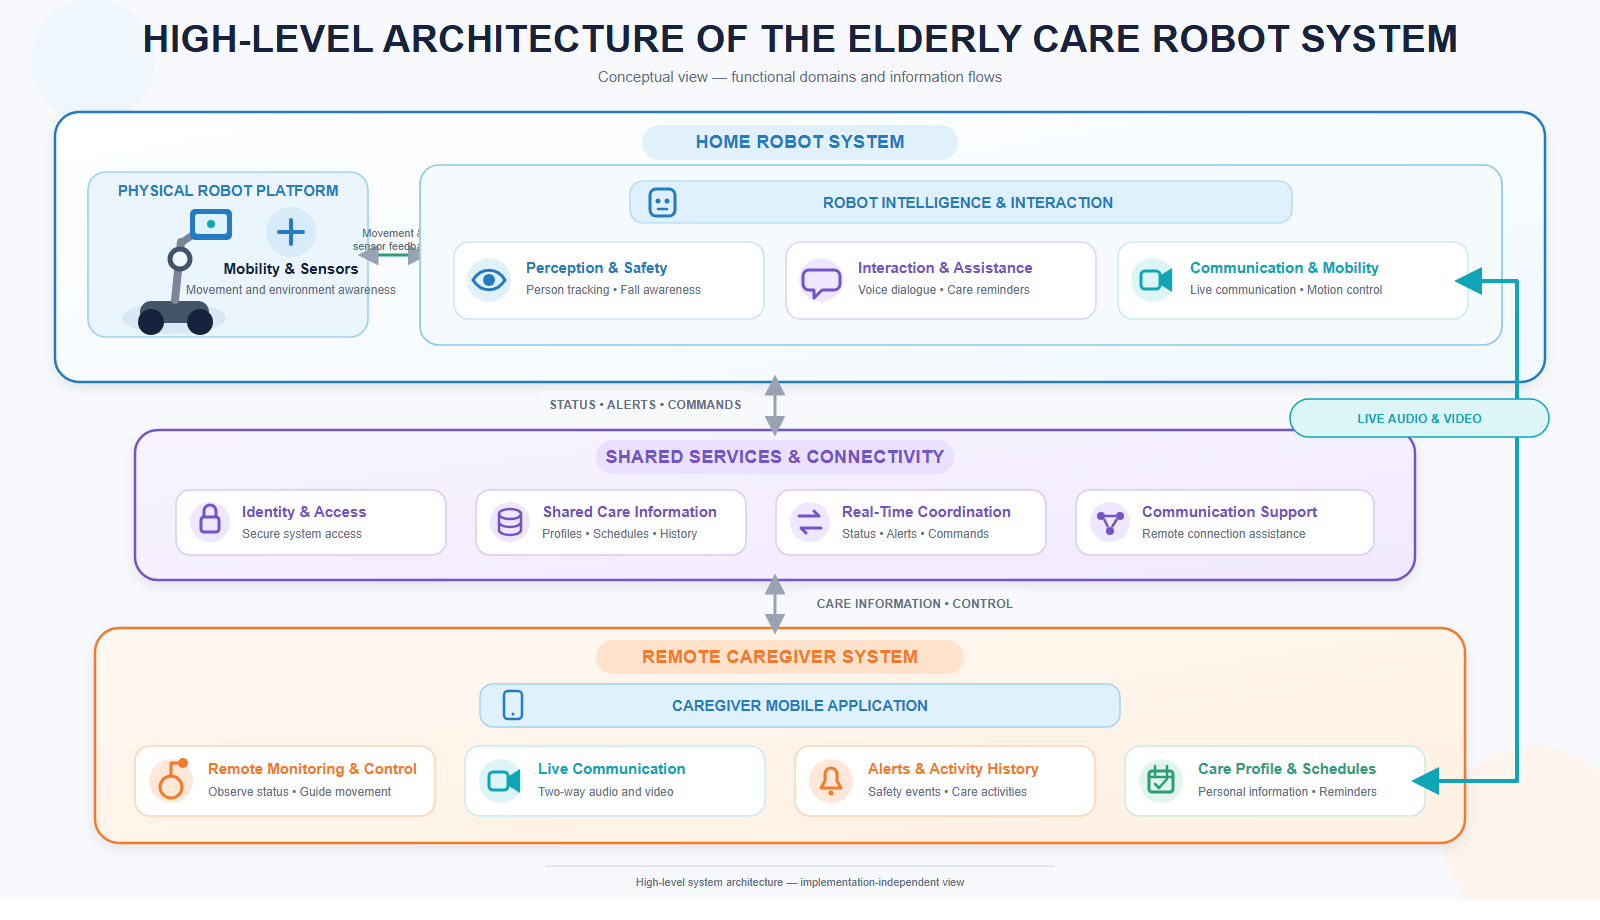
\includegraphics[width=\textwidth]{High_Level_System_Architecture.png}
    \caption{Kiến trúc tổng quan của hệ thống robot hỗ trợ chăm sóc người cao tuổi}
    \label{fig:high_level_architecture}
\end{figure}

\subsubsection{Các module và trách nhiệm}

Các thành phần trong kiến trúc được chia thành những module có nhiệm vụ và dữ liệu trao đổi xác định. Bảng \ref{tab:logical_modules} tổng hợp đầu vào, chức năng xử lý và đầu ra của từng module, qua đó làm rõ cách các thành phần phối hợp trong quá trình vận hành.

\begin{longtable}{|p{3.1cm}|p{3.7cm}|p{3.8cm}|p{3.0cm}|}
\caption{Các module trong kiến trúc tổng quan của hệ thống}\label{tab:logical_modules}\\
\hline
\textbf{Module} & \textbf{Đầu vào} & \textbf{Xử lý/trách nhiệm} & \textbf{Đầu ra} \\
\hline
\endfirsthead
\hline
\textbf{Module} & \textbf{Đầu vào} & \textbf{Xử lý/trách nhiệm} & \textbf{Đầu ra} \\
\hline
\endhead
Quản lý chăm sóc & Thao tác cập nhật hồ sơ, lịch và trạng thái chức năng & Kiểm tra dữ liệu nhập, cập nhật cấu hình và truy vấn lịch sử & Hồ sơ, lịch, trạng thái giám sát \\
\hline
Giám sát và can thiệp từ xa & Cảnh báo, video và thao tác trên cần điều khiển ảo & Hiển thị tình trạng, nhận cuộc gọi và tạo lệnh điều khiển & Phản hồi cuộc gọi, vector điều khiển \\
\hline
Điều phối RobotApp & Thao tác người dùng, lịch, trạng thái chức năng và kết quả AI & Quản lý camera, kết nối BLE, lựa chọn nguồn lệnh và phối hợp xử lý sự kiện & Yêu cầu hội thoại, cuộc gọi hoặc lệnh chuyển động \\
\hline
Cảm nhận và định danh mục tiêu & Khung hình camera & Ước lượng tư thế, liên kết kết quả phát hiện giữa các khung hình và duy trì mục tiêu ID0 & Hộp bao, điểm khớp và định danh mục tiêu \\
\hline
Theo dõi chuyển động & Vị trí mục tiêu ID0 và cấu hình bám theo & Ước lượng độ gần, điều chỉnh hướng và xử lý khi mất dấu & Vector tiến, lùi, quay hoặc lệnh dừng \\
\hline
Phát hiện và xác nhận té ngã & Chuỗi tư thế của mục tiêu ID0 & Phân loại chuỗi, kiểm tra bổ sung và yêu cầu người dùng xác nhận tình trạng & Kết quả xác nhận an toàn hoặc sự kiện cảnh báo \\
\hline
Hội thoại và lời nhắc & Giọng nói, hồ sơ, lịch và sự kiện té ngã & Chuyển tiếng nói thành văn bản, tạo câu trả lời, tổng hợp tiếng nói và ghi nhận phản hồi & Âm thanh, yêu cầu của người dùng và trạng thái phản hồi \\
\hline
Liên lạc thời gian thực & Yêu cầu gọi và thông tin thiết lập phiên & Thiết lập, kết thúc cuộc gọi, quản lý camera và truyền âm thanh, hình ảnh hai chiều & Âm thanh, hình ảnh và trạng thái cuộc gọi \\
\hline
Dữ liệu và điều phối dùng chung & Hồ sơ, lịch, trạng thái chức năng, lệnh, cảnh báo và thông tin cuộc gọi & Xác thực, phân vùng dữ liệu và đồng bộ thay đổi giữa hai thiết bị & Dữ liệu cập nhật của từng cặp thiết bị \\
\hline
Cầu nối điều khiển & Vector điều khiển từ xa hoặc bám theo tự động & Chọn nguồn lệnh, kiểm tra giá trị và thời điểm tạo lệnh, tính vận tốc hai bánh & Vận tốc đặt của bánh trái và bánh phải \\
\hline
Chấp hành thân robot & Vận tốc đặt của hai bánh và góc rotor & Điều khiển vận tốc vòng kín, giới hạn lệnh và dừng khi quá thời gian chờ & Tín hiệu PWM điều khiển động cơ và trạng thái dừng \\
\hline
Chuẩn bị mô hình ngoại tuyến & Mô hình đã huấn luyện và cấu hình chuyển đổi & Chuyển đổi định dạng, kiểm tra tensor và tạo mô hình cho thiết bị di động & Mô hình sẵn sàng triển khai \\
\hline
\end{longtable}

Kết quả nhận dạng của AI được chuyển đến các module xử lý để xác định phản ứng phù hợp của robot. Chẳng hạn, mô hình ước lượng tư thế cung cấp các điểm khớp, còn LSTM trả về xác suất té ngã; bộ hậu kiểm sử dụng các kết quả này để quyết định có cần hỏi xác nhận hay không. Module điều phối tiếp tục xử lý việc dừng robot, ghi cảnh báo và gọi người chăm sóc. Đối với chuyển động, cần điều khiển ảo và chức năng bám theo tạo vector điều khiển chuẩn hóa; module cầu nối kiểm tra tính hợp lệ của lệnh rồi chuyển thành vận tốc đặt cho hai động cơ. Cách phân chia này giúp tập trung các điều kiện kiểm tra trước khi robot thực hiện hành động.

\subsection{Các luồng xử lý chính}

\subsubsection{Các trường hợp sử dụng chính}

Các trường hợp sử dụng được chia thành bốn nhóm: quản lý hồ sơ, lịch nhắc nhở và nhật ký; hội thoại và thực hiện lời nhắc; giám sát, bám theo và phát hiện té ngã; liên lạc và điều khiển robot. Người chăm sóc chủ yếu thao tác thông qua ứng dụng quản lý, trong khi người cao tuổi tương tác trực tiếp với robot bằng giọng nói và tham gia cuộc gọi khi cần. Bảng \ref{tab:usecases} tóm tắt tác nhân và kết quả của các trường hợp sử dụng chính.

\begin{table}[htbp]
\centering
\caption{Tóm tắt các trường hợp sử dụng chính}
\label{tab:usecases}
\small
\begin{tabularx}{\textwidth}{|p{1.3cm}|p{4.0cm}|p{3.0cm}|X|}
\hline
\textbf{Mã} & \textbf{Trường hợp sử dụng} & \textbf{Tác nhân chính} & \textbf{Kết quả} \\
\hline
UC01 & Đăng ký/đăng nhập & Người chăm sóc, thiết bị robot & Phiên Firebase và UID dùng chung cho cặp thiết bị \\
\hline
UC02 & Quản lý hồ sơ & Người chăm sóc & Hồ sơ và ngữ cảnh xưng hô được cập nhật \\
\hline
UC03 & Quản lý lịch nhắc nhở & Người chăm sóc & Lịch được đồng bộ tới RobotApp \\
\hline
UC04 & Nhận và xác nhận lời nhắc & Người cao tuổi & Nội dung được phát và phản hồi được ghi nhật ký \\
\hline
UC05 & Hội thoại trợ lý & Người cao tuổi & Câu trả lời được tạo và phát bằng giọng nói \\
\hline
UC06 & Bật/tắt giám sát & Người chăm sóc & Auto-follow hoặc phát hiện té ngã thay đổi trạng thái \\
\hline
UC07 & Phát hiện và xác nhận té ngã & Người cao tuổi, RobotApp & Loại nhiễu, xác nhận an toàn hoặc kích hoạt cảnh báo \\
\hline
UC08 & Gọi video & Hai người dùng & Phiên WebRTC được thiết lập và kết thúc \\
\hline
UC09 & Điều khiển robot & Người chăm sóc & Lệnh hợp lệ tới hai động cơ hoặc STOP \\
\hline
UC10 & Xem nhật ký & Người chăm sóc & Danh sách lời nhắc, cảnh báo và cuộc gọi \\
\hline
\end{tabularx}
\end{table}

\clearpage
\subsubsection{Luồng giám sát và xử lý té ngã}

Hình \ref{fig:activity_fall_detection} mô tả quá trình giám sát sau khi người chăm sóc bật chức năng phát hiện té ngã. Mỗi khung hình hợp lệ được xử lý qua mô hình YOLO-Pose, bộ theo dõi và LSTM. Khi có ít nhất năm kết quả FALL liên tiếp, hệ thống ghi nhận một chuỗi nghi té ngã nhưng chưa phát cảnh báo. Kết quả NO FALL đầu tiên kết thúc chuỗi và bắt đầu bước kiểm tra vị trí mũi, vai. Nếu các điểm thân trên nằm trong vùng 70\% phía trên ảnh ở ba khung hình kiểm tra liên tiếp, tình huống nghi té ngã được loại bỏ; nếu nằm dưới ngưỡng này trong ba khung hình liên tiếp, hệ thống chuyển sang hỏi xác nhận. Khi không còn quan sát được mục tiêu hoặc các điểm thân trên trong 12 khung hình liên tiếp, hệ thống cũng hỏi xác nhận tình trạng người dùng.

Khi cần xác nhận, RobotApp đánh dấu sự kiện đang được xử lý, dừng chuyển động và chuyển sang hội thoại với người cao tuổi. Nếu người dùng trả lời rõ ràng rằng mình an toàn, sự kiện được kết thúc tại robot và không tạo bản ghi cảnh báo. Nếu câu trả lời cho thấy cần hỗ trợ, chưa rõ nghĩa, xảy ra lỗi phân loại hoặc không có phản hồi trong 10 s, ứng dụng tạo bản ghi tại \path|fall_alerts| và khởi tạo cuộc gọi khẩn cấp. Bộ hậu kiểm chỉ trở về trạng thái giám sát sau 10 kết quả NO FALL liên tiếp để hạn chế yêu cầu xác nhận trùng lặp.

\begin{figure}[H]
    \centering
    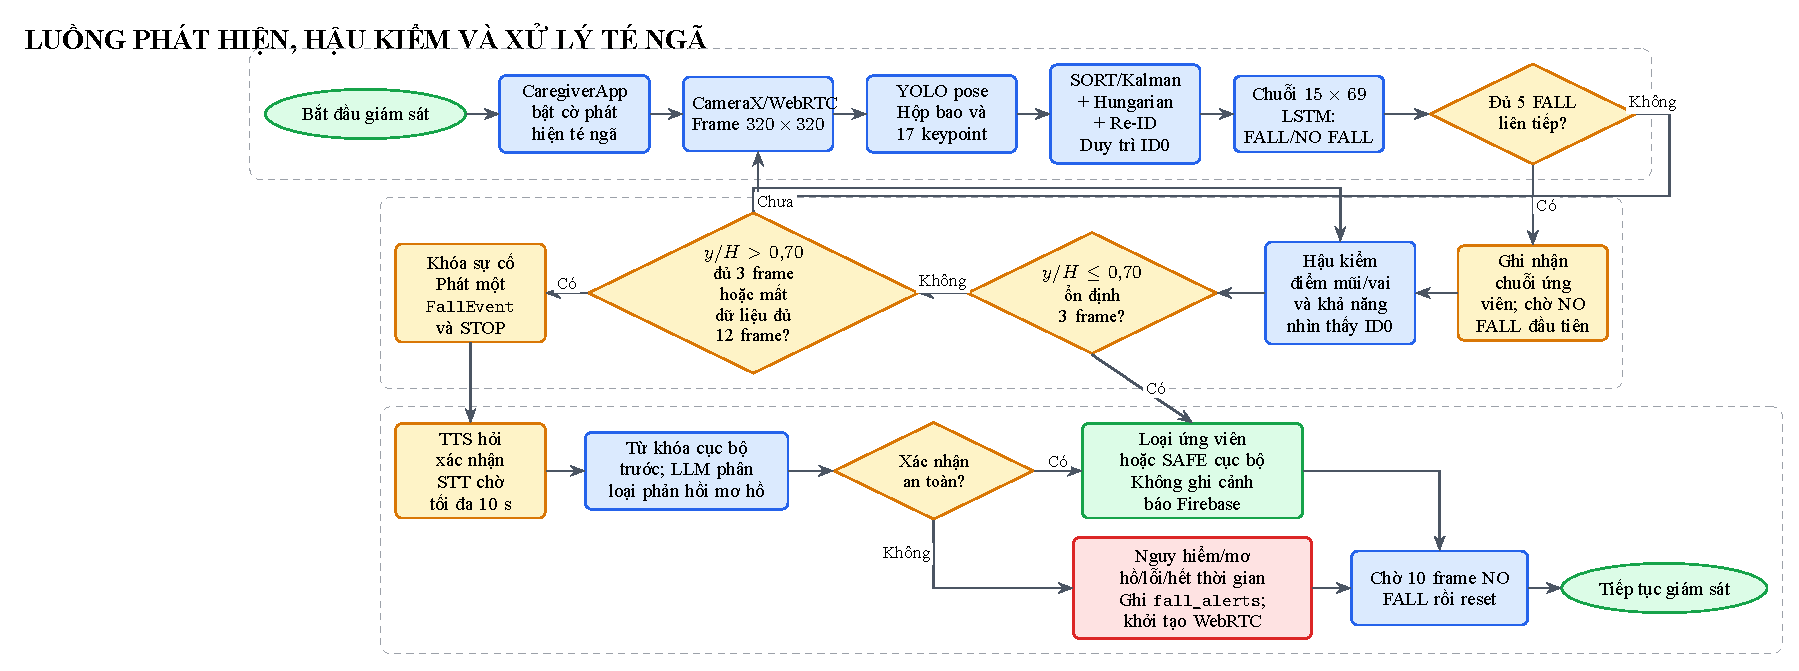
\includegraphics[width=\textwidth]{Images/Activity_Fall_Detection.pdf}
    \caption{Biểu đồ hoạt động của quy trình phát hiện, hậu kiểm và xử lý té ngã}
    \label{fig:activity_fall_detection}
\end{figure}

\clearpage
\subsubsection{Luồng cuộc gọi khẩn cấp và điều khiển từ xa}

Hình \ref{fig:sequence_emergency_response} trình bày quá trình trao đổi giữa người cao tuổi, RobotApp, khối xử lý AI, ESP32, Firebase và CaregiverApp. Khối AI cung cấp kết quả phân tích; RobotApp điều phối việc dừng chuyển động, hỏi xác nhận, lưu cảnh báo và mở màn hình gọi. Khi cần liên lạc, RobotApp ghi \texttt{status=calling}, \texttt{callerRole=robot}, \texttt{emergencyReason=fall} cùng bản mô tả phiên SDP đề nghị vào nhánh báo hiệu của cặp thiết bị. CaregiverApp tiếp nhận yêu cầu gọi và tạo bản mô tả phiên trả lời; hai phía sau đó trao đổi các địa chỉ kết nối ứng viên ICE.

Sau khi kết nối WebRTC được thiết lập, âm thanh và hình ảnh được truyền trực tiếp giữa hai thiết bị hoặc chuyển tiếp qua máy chủ TURN. Khi người chăm sóc sử dụng cần điều khiển ảo, lệnh đi theo chuỗi CaregiverApp $\rightarrow$ RTDB $\rightarrow$ RobotApp $\rightarrow$ BLE $\rightarrow$ ESP32. Các lệnh từ xa vẫn phải qua bước kiểm tra thời điểm tạo lệnh và cơ chế dừng khi không còn cập nhật.

\begin{sidewaysfigure}
    \centering
    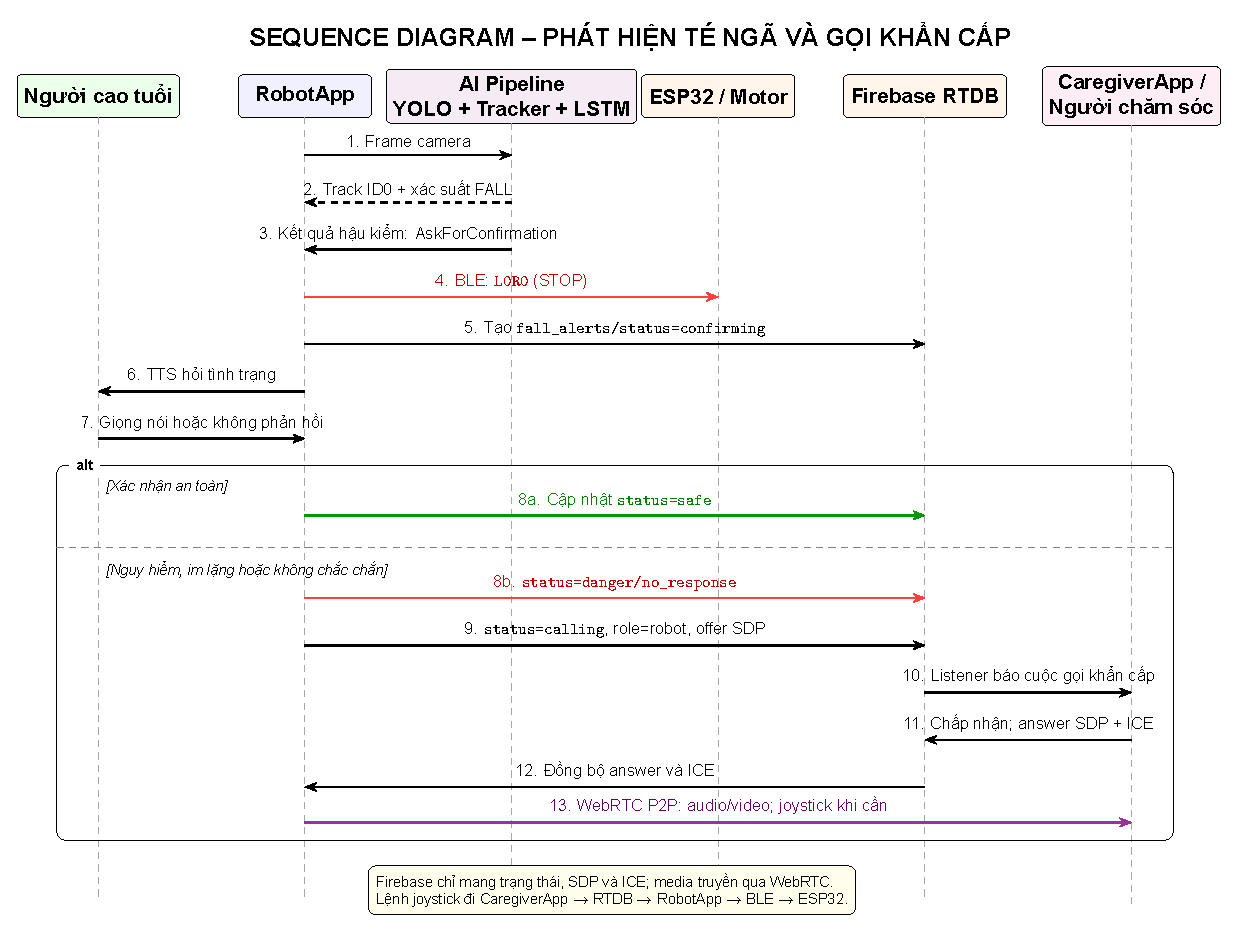
\includegraphics[width=0.92\textheight]{Images/Sequence_Emergency_Response.pdf}
    \caption{Biểu đồ tuần tự của quá trình phát hiện té ngã và thiết lập cuộc gọi khẩn cấp}
    \label{fig:sequence_emergency_response}
\end{sidewaysfigure}

\clearpage
\subsubsection{Luồng hội thoại và nhắc nhở}

Trong hội thoại thông thường, bộ nhận dạng tiếng nói chuyển lời nói thành văn bản. \texttt{GroqChatService} kết hợp câu hỏi với hồ sơ người dùng và lịch sử hội thoại gần nhất để gửi đến LLM, sau đó tiếp nhận từng phần nội dung trả lời. RobotApp ghép các phần này thành câu hoàn chỉnh và đưa vào hàng đợi tổng hợp tiếng nói, nhờ đó có thể bắt đầu trả lời trước khi nhận đủ toàn bộ nội dung. Khi phát xong câu trả lời, ứng dụng trở lại trạng thái lắng nghe.

Đối với lịch nhắc nhở, CaregiverApp lưu cấu hình tại \path|Schedules/{uid}|. \texttt{ReminderService} trên RobotApp kiểm tra lịch mỗi 30 s, đối chiếu thời điểm và chế độ lặp, tạo bản ghi ở trạng thái \texttt{delivered}, rồi gửi sự kiện đến chatbot để phát lời nhắc. LLM hỗ trợ tạo cách diễn đạt thân thiện, trong khi tiêu đề và ghi chú vẫn được lấy từ lịch đã thiết lập. Phản hồi của người dùng và số lần nhắc lại được cập nhật vào cùng bản ghi để người chăm sóc theo dõi.

\subsection{Thiết kế và lựa chọn công nghệ cho các module}

Sau khi xác định các module và luồng phối hợp, những công nghệ phù hợp được lựa chọn dựa trên độ trễ, tài nguyên của điện thoại, khả năng tích hợp và phạm vi hệ thống. Mỗi loại dữ liệu có đặc điểm riêng: giải pháp phù hợp để lưu trữ hồ sơ chưa chắc đáp ứng việc truyền video thời gian thực, còn một mô hình đạt độ chính xác cao trên máy trạm có thể không duy trì được tốc độ suy luận trên điện thoại. Bảng \ref{tab:crosscutting_technology_choices} tóm tắt các quyết định nền tảng; các mục tiếp theo trình bày thiết kế chi tiết của từng khối.

\begin{longtable}{|p{2.8cm}|p{3.4cm}|p{3.5cm}|p{3.8cm}|}
\caption{So sánh các lựa chọn công nghệ xuyên suốt hệ thống}\label{tab:crosscutting_technology_choices}\\
\hline
\textbf{Bài toán} & \textbf{Phương án xem xét} & \textbf{Ưu điểm và hạn chế chính} & \textbf{Lựa chọn cho đề tài} \\
\hline
\endfirsthead
\hline
\textbf{Bài toán} & \textbf{Phương án xem xét} & \textbf{Ưu điểm và hạn chế chính} & \textbf{Lựa chọn cho đề tài} \\
\hline
\endhead
Ứng dụng di động & Phát triển trực tiếp trên Android; nền tảng phát triển đa hệ điều hành; ứng dụng web & Phát triển trực tiếp trên Android thuận tiện khi tích hợp camera, BLE và dịch vụ nền; nền tảng đa hệ điều hành hỗ trợ dùng chung mã giao diện nhưng có thể cần lớp tích hợp riêng & Kotlin, XML và ViewBinding cho hai ứng dụng Android \\
\hline
Suy luận AI & Suy luận trên máy chủ; suy luận tại thiết bị & Máy chủ thuận tiện nâng cấp mô hình nhưng cần truyền ảnh qua mạng; xử lý tại thiết bị giảm phụ thuộc mạng và hạn chế truyền ảnh ra ngoài, song chịu giới hạn tài nguyên & TFLite trên RobotApp, ưu tiên GPU/NNAPI và có CPU dự phòng \reportcite{ref:tflite} \\
\hline
Đồng bộ dữ liệu & REST tự xây dựng; MQTT; cơ sở dữ liệu thời gian thực & REST cho phép kiểm soát cao nhưng cần xây dựng máy chủ; MQTT phù hợp dữ liệu đo và điều khiển nhưng cần broker cùng cơ chế lưu trữ bổ sung; RTDB cung cấp listener và cây JSON nhưng đòi hỏi quản lý chặt cấu trúc dữ liệu và quy tắc truy cập & Firebase Authentication và Realtime Database cho mô hình một cặp thiết bị \reportcite{ref:firebase_rtdb} \\
\hline
Truyền âm thanh và hình ảnh & Truyền qua cơ sở dữ liệu; máy chủ truyền phát tập trung; WebRTC & Cơ sở dữ liệu không phù hợp truyền hình liên tục; máy chủ tập trung cần thêm hạ tầng; WebRTC hỗ trợ liên lạc thời gian thực nhưng cần quản lý báo hiệu và phiên kết nối & WebRTC truyền âm thanh, hình ảnh; RTDB trao đổi thông tin thiết lập cuộc gọi \reportcite{ref:webrtc} \\
\hline
Liên kết điện thoại--thân robot & USB; BLE & USB có độ ổn định cao nhưng ràng buộc thiết bị bằng cáp; BLE phù hợp với các gói lệnh điều khiển có kích thước nhỏ, tiêu thụ ít năng lượng và hỗ trợ kết nối không dây trong phạm vi gần, song có băng thông hạn chế & BLE GATT vì dữ liệu điều khiển có kích thước nhỏ và không bao gồm hình ảnh \reportcite{ref:ble_primer} \\
\hline
Hội thoại & Mô hình cục bộ; LLM qua API; kịch bản cố định & Mô hình cục bộ cần nhiều tài nguyên; LLM qua API hỗ trợ hội thoại linh hoạt nhưng phụ thuộc mạng và chi phí; kịch bản cố định dễ kiểm soát nhưng hạn chế nội dung & Android STT/TTS kết hợp LLM qua API, bổ sung từ khóa nhận biết phản hồi và câu mẫu dự phòng \\
\hline
\end{longtable}

\subsubsection{Module ứng dụng người chăm sóc và điều phối tại robot}

CaregiverApp đảm nhiệm vai trò giao diện quản lý từ xa với bốn nhóm chức năng: hồ sơ và lịch nhắc nhở, cấu hình giám sát, cuộc gọi kèm cần điều khiển ảo, và tra cứu nhật ký. Ứng dụng tiếp nhận thao tác của người chăm sóc, đồng bộ cấu hình, gửi lệnh và xử lý yêu cầu cuộc gọi. Các tác vụ ước lượng tư thế, hội thoại chính và kết nối ESP32 không được đặt tại đây, nhờ đó thiết bị của người chăm sóc không phụ thuộc vào mô hình TFLite hoặc trình điều khiển BLE của robot.

RobotApp điều phối các chức năng trên robot. Ứng dụng tiếp nhận khung hình, âm thanh, lịch nhắc nhở, trạng thái chức năng và lệnh từ xa, sau đó chuyển dữ liệu đến module tương ứng. Kết quả nhận dạng và dự đoán của AI được kết hợp với trạng thái xử lý hiện tại để quyết định dừng robot, hỏi xác nhận hoặc mở cuộc gọi. Kết nối BLE được quản lý tập trung để tránh nhiều thành phần đồng thời tạo kết nối GATT tới ESP32; CameraX và WebRTC luân phiên sử dụng camera theo trạng thái cuộc gọi.

Trong phạm vi đề tài, hai ứng dụng được phát triển trực tiếp trên nền tảng Android bằng Kotlin và XML. Android cung cấp các giao diện lập trình để sử dụng camera, microphone, Bluetooth, nhận dạng và tổng hợp tiếng nói, đồng thời hỗ trợ tổ chức các tác vụ nền. Những khả năng này phù hợp với yêu cầu tích hợp chức năng giám sát, hội thoại và kết nối thân robot. Phần giao diện, xử lý nghiệp vụ và tác vụ nền được phân chia theo chức năng để thuận tiện kiểm thử và bảo trì. Hệ thống hiện hướng đến các thiết bị Android được sử dụng trong đồ án.

\subsubsection{Module thu nhận hình ảnh, ước lượng tư thế và theo dõi mục tiêu}

Để giám sát và phát hiện té ngã trên điện thoại gắn trên robot, module thị giác cần cung cấp đồng thời hộp bao người và các điểm khớp cơ thể với tốc độ phù hợp cho việc phân tích chuyển động theo thời gian. Việc kết hợp một bộ phát hiện người với một mô hình ước lượng tư thế riêng cho phép thay thế từng thành phần độc lập, nhưng cần hai lượt suy luận và bước chuyển vùng ảnh giữa hai mô hình. Mô hình tích hợp phát hiện người và ước lượng tư thế tạo cả hai loại kết quả trong cùng một lượt suy luận, giúp đơn giản hóa chuỗi xử lý.

Các mô hình MobileNet SSD và EfficientDet tiêu chuẩn phục vụ phát hiện đối tượng nhưng không trực tiếp cung cấp 17 điểm khớp, nên cần thêm mô hình ước lượng tư thế. YOLO-Pose cung cấp đồng thời hộp bao và điểm khớp, đồng thời hỗ trợ xuất sang TFLite/LiteRT \reportcite{ref:yolo_pose_docs}. Từ quy trình ở Mục \ref{sec:yolo_pose_inference_pipeline}, cấu trúc đầu vào, đầu ra ở Mục \ref{sec:yolo_pose_output_representation} và so sánh quy mô ở Mục \ref{sec:yolo26_pose_scales}, đề tài lựa chọn YOLO26n-Pose. Biến thể nano có số tham số và chi phí tính toán thấp nhất trong các mức n, s, m, l và x, phù hợp với điện thoại còn phải thực hiện theo dõi, hội thoại, đồng bộ dữ liệu và điều khiển. Tuy nhiên, chỉ số mAP ước lượng tư thế thấp hơn các biến thể lớn, nên lựa chọn này cần được đánh giá thêm về độ trễ và chất lượng điểm khớp trên thiết bị sử dụng.

Module nhận khung hình từ CameraX hoặc bản sao hình ảnh của WebRTC. Ảnh được đổi về kích thước $320\times320$ trước khi suy luận bằng YOLO-Pose. Kết quả được lọc với ngưỡng tin cậy 0,20, ngưỡng IoU của bước NMS là 0,45 và ngưỡng hiển thị điểm khớp là 0,30. Hộp bao người và 17 điểm khớp được dùng chung cho theo dõi mục tiêu, ước lượng độ gần và phân tích bằng LSTM. Tần suất xử lý được đặt giới hạn trên ở 25 FPS; nếu lượt suy luận trước chưa hoàn tất, khung hình mới được bỏ qua để hạn chế tích lũy độ trễ.

Việc gửi khung hình lên dịch vụ đám mây cho phép sử dụng phần cứng mạnh hơn, nhưng làm tăng độ trễ, băng thông và rủi ro đối với dữ liệu hình ảnh. Suy luận trực tiếp trên điện thoại chịu giới hạn về tài nguyên nhưng đáp ứng tốt hơn NFR02, NFR06 và vẫn hoạt động khi Internet gián đoạn. Vì vậy, TFLite được chọn làm môi trường suy luận trên thiết bị; hệ thống ưu tiên GPU, chuyển sang NNAPI khi cần và sử dụng CPU bốn luồng làm phương án cuối \reportcite{ref:tflite}.

Đối với theo dõi người, SORT có cấu trúc gọn và tốc độ xử lý cao nhưng phụ thuộc vào chất lượng phát hiện. ByteTrack tận dụng thêm các kết quả có độ tin cậy thấp để duy trì đối tượng khi bị che khuất, đồng thời cần thêm bước liên kết kết quả \reportcite{ref:sort}\reportcite{ref:bytetrack}. Mạng tái định danh dựa trên học sâu có thể phân biệt ngoại hình tốt hơn, nhưng làm tăng dung lượng mô hình và thời gian suy luận. Đề tài sử dụng cấu trúc SORT với bộ lọc Kalman và thuật toán Hungarian, bổ sung khoảng cách giữa các điểm khớp và biểu đồ phân bố màu H--S khi cần nhận lại mục tiêu. Hàm chi phí liên kết được xác định như sau:

\begin{equation}
C=0,30(1-\operatorname{IoU})+0,30\hat d_c+0,30\hat d_p+0,10p_a,
\end{equation}

trong đó $\hat d_c$ là khoảng cách tâm đã chuẩn hóa, $\hat d_p$ là khoảng cách giữa các điểm mốc tại vai và hông, còn $p_a$ là thành phần chi phí phản ánh sự thay đổi diện tích hộp bao. Khi lựa chọn người mục tiêu ban đầu, mỗi đối tượng được đánh giá theo điểm số:

\begin{equation}
Q=0,60q_{area}+0,15q_{det}+0,15q_{vis}+0,10q_{center}-p_{edge}.
\end{equation}

Trong biểu thức trên, $q_{area}$ phản ánh diện tích hộp bao, $q_{det}$ là độ tin cậy phát hiện, $q_{vis}$ phản ánh tỷ lệ điểm khớp quan sát được, $q_{center}$ biểu diễn mức độ gần tâm ảnh và $p_{edge}$ là thành phần giảm điểm khi người bị cắt ở biên ảnh. Đối tượng có điểm số cao nhất được gán định danh ID0 để dùng chung cho bám theo và phát hiện té ngã. Bộ theo dõi duy trì ID0 tối đa 45 khung hình không ghép được với kết quả phát hiện; các định danh khác được giữ tối đa 10 khung hình. Cơ chế tìm lại mục tiêu hoạt động trong khoảng 2 s, với điều kiện đối tượng nằm cách vị trí cuối không quá 35\% đường chéo ảnh, thuộc vùng trung tâm và được quan sát ổn định trong ba khung hình. Khi đang xử lý một sự kiện nghi té ngã, hệ thống không tự chuyển sang người khác.

\subsubsection{Module tự bám theo và điều khiển chuyển động}

Module bám theo tự động nhận hộp bao và các điểm khớp của mục tiêu ID0, sau đó tạo vector điều khiển tịnh tiến và quay đã chuẩn hóa. Độ gần được ước lượng từ diện tích hộp bao và các mốc vai, hông, gối, mắt cá chân, rồi làm mượt bằng trung bình trượt lũy thừa (Exponential Moving Average -- EMA). Giá trị này được chia thành ba vùng: quá xa, phù hợp và quá gần. Ngưỡng đi vào và rời khỏi mỗi vùng được đặt khác nhau để hạn chế việc robot đổi trạng thái liên tục khi giá trị dao động gần biên. Sai lệch ngang giữa tâm mục tiêu và tâm ảnh tạo thành phần quay, với vùng chết 0,07, hệ số 2,2 và giới hạn độ lớn 0,50. Vector điều khiển được cập nhật khoảng mỗi 120 ms.

Bộ điều khiển chỉ dựa vào tâm hộp bao có chi phí tính toán thấp, nhưng có thể đánh giá sai khoảng cách khi phần chân bị cắt khỏi ảnh. Cảm biến chiều sâu cung cấp khoảng cách trực tiếp hơn nhưng làm tăng độ phức tạp phần cứng và nằm ngoài phạm vi đề tài. Do đó, hệ thống kết hợp hộp bao với các keypoint và áp dụng chính sách chuyển động thận trọng: khi vùng bao quá lớn hoặc phần chân không còn trong khung hình, robot ưu tiên lùi để quan sát đầy đủ hơn. Sau khi xuất hiện kết quả FALL, robot không tiến về phía người mà chỉ dừng, lùi chậm hoặc quay tại chỗ; nếu mất ID0 trong trạng thái này, robot dừng ngay.

Lệnh từ cần điều khiển ảo và chức năng bám theo tự động sử dụng chung cấu trúc $x,y,ts$, nhưng chỉ một nguồn được quyền điều khiển tại một thời điểm. Module cầu nối tập trung việc kiểm tra thời điểm tạo lệnh, giới hạn giá trị và dừng khi quá thời gian chờ, giúp áp dụng cùng một quy trình kiểm tra cho cả hai nguồn.

\subsubsection{Module phát hiện, hậu kiểm và xác nhận té ngã}

Bài toán phát hiện té ngã có thể được tiếp cận bằng ngưỡng hình học trên từng khung hình, mô hình phân loại trực tiếp từ ảnh hoặc đoạn video, hoặc mô hình phân tích chuỗi điểm khớp. Ngưỡng hình học có chi phí tính toán thấp và dễ giải thích nhưng nhạy với góc nhìn. Mô hình học trực tiếp từ video có thể khai thác cả hình ảnh và chuyển động, song cần nhiều tài nguyên và dữ liệu huấn luyện. Chuỗi điểm khớp có kích thước đầu vào nhỏ hơn và thể hiện được diễn biến tư thế, nhưng phụ thuộc vào chất lượng ước lượng các điểm này. Đề tài lựa chọn YOLO-Pose kết hợp LSTM, sau đó kiểm tra bổ sung theo quy tắc và hỏi xác nhận bằng giọng nói để hạn chế cảnh báo nhầm.

Mỗi khung hình của mục tiêu ID0 được chuyển thành vector 69 đặc trưng:

\begin{equation}
\mathbf f_t=[x_i,y_i,\Delta x_i,\Delta y_i]_{i=1}^{17}\oplus r_t,
\end{equation}

trong đó tọa độ điểm khớp được chuẩn hóa theo tâm hông và kích thước vùng tư thế, $\Delta x_i,\Delta y_i$ là độ dịch chuyển so với khung hình trước, còn $r_t$ là tỷ lệ rộng/cao. Cửa sổ 15 khung hình tạo tensor $[1,15,69]$; LSTM trả về $[p_{normal},p_{fall}]$ và kết quả được gán nhãn FALL khi $p_{fall}>p_{normal}$. LSTM khai thác quan hệ theo thời gian của chuỗi tư thế để bổ sung thông tin chuyển động cho việc phân loại \reportcite{ref:lstm}.

Bộ hậu kiểm quản lý quá trình xử lý qua các trạng thái \texttt{MONITORING}, \texttt{FALL\_SEQUENCE}, \texttt{VERIFYING}, \texttt{PROMPTED}, \texttt{DISMISSED} và \texttt{CONFIRMED}, tương ứng với giám sát, ghi nhận chuỗi nghi té ngã, kiểm tra bổ sung, hỏi xác nhận, loại bỏ sự kiện và xác nhận nguy hiểm. Năm kết quả FALL liên tiếp hình thành một chuỗi nghi té ngã. Sau kết quả NO FALL đầu tiên, ba khung hình liên tiếp có điểm mũi hoặc vai ở $y/H\leq0,70$ sẽ loại bỏ sự kiện; ba khung hình liên tiếp có các điểm này ở $y/H>0,70$, hoặc 12 khung hình liên tiếp không quan sát được mục tiêu hay phần thân trên, sẽ dẫn đến bước hỏi xác nhận. Nếu câu trả lời chưa rõ nghĩa, xảy ra lỗi phân loại hoặc hết 10 s chờ phản hồi, hệ thống xử lý theo trường hợp cần hỗ trợ. Sau khi sự kiện được kết luận, bộ hậu kiểm chỉ trở về trạng thái giám sát khi ghi nhận 10 kết quả NO FALL liên tiếp, nhằm hạn chế yêu cầu xác nhận trùng lặp. Các bước kiểm tra bổ sung tạo thêm độ trễ, đổi lại giúp hệ thống xem xét diễn biến qua nhiều khung hình trước khi phát cảnh báo.

\subsubsection{Module hội thoại và lời nhắc}

Mô hình hội thoại chạy hoàn toàn tại thiết bị hạn chế phụ thuộc mạng và việc gửi dữ liệu ra ngoài, nhưng cần chia sẻ tài nguyên với chức năng thị giác. Phương án dùng kịch bản cố định có chi phí xử lý thấp và dễ kiểm soát nội dung, song khó đáp ứng hội thoại hằng ngày với nhiều chủ đề. Vì vậy, đề tài kết hợp Android SpeechRecognizer để chuyển tiếng nói thành văn bản, LLM qua API để tạo câu trả lời và Android TextToSpeech để tổng hợp tiếng nói \reportcite{ref:android_speech}\reportcite{ref:groq_api}\reportcite{ref:android_tts}. Những phản hồi thể hiện rõ tình trạng an toàn hoặc nguy hiểm được nhận biết trước bằng từ khóa tại thiết bị; chức năng nhắc nhở sử dụng câu mẫu dự phòng khi không nhận được phản hồi từ API.

Hoạt động hội thoại được tổ chức theo các trạng thái nghỉ, lắng nghe, xử lý câu hỏi, phát câu trả lời, xác nhận lời nhắc, xác nhận té ngã và đang gọi. Hồ sơ người dùng được bổ sung vào phần chỉ dẫn cho LLM; lịch sử hội thoại giới hạn ở 20 thông điệp để kiểm soát độ dài ngữ cảnh. Phản hồi được tiếp nhận từng phần, ghép thành câu rồi đưa vào TTS, giúp rút ngắn thời gian từ khi đặt câu hỏi đến khi robot bắt đầu trả lời. Các tác vụ ngắn, như phân loại phản hồi hoặc nhận biết yêu cầu gọi, sử dụng yêu cầu riêng nhận kết quả đầy đủ trong một lần và không thêm vào lịch sử trò chuyện. Module nhắc nhở kiểm tra lịch mỗi 30 s, tạo bản ghi trước khi phát sự kiện và giữ nguyên nội dung lịch đã thiết lập.

\subsubsection{Module dữ liệu dùng chung và liên lạc thời gian thực}

Firebase Realtime Database được lựa chọn để đồng bộ các dữ liệu có kích thước nhỏ như trạng thái chức năng, lệnh điều khiển và sự kiện. Các bộ lắng nghe thông báo thay đổi đến hai ứng dụng gần thời gian thực, kết hợp với Firebase Authentication để xác định tài khoản truy cập. Giải pháp này giảm khối lượng xây dựng máy chủ riêng so với REST hoặc việc bổ sung cơ chế lưu trữ cho MQTT. Tuy nhiên, hai ứng dụng cần thống nhất cấu trúc cây JSON và đường dẫn; việc thay đổi cấu trúc dữ liệu phải được cập nhật đồng bộ. Các đường dẫn vì vậy được quản lý tập trung và phân vùng theo UID; lệnh điều khiển kèm thời điểm tạo để kiểm tra hiệu lực. Hai thiết bị dùng chung tài khoản nên hệ thống hiện chưa phân quyền riêng cho robot và người chăm sóc \reportcite{ref:firebase_rtdb}\reportcite{ref:firebase_security}.

Âm thanh và hình ảnh được truyền bằng WebRTC, còn RTDB lưu trạng thái và thông tin thiết lập cuộc gọi, gồm bản mô tả phiên đề nghị, bản trả lời và hai nhánh địa chỉ ứng viên ICE. WebRTC hỗ trợ kết nối trực tiếp khi điều kiện mạng cho phép và chuyển tiếp qua TURN khi cần. Quá trình tích hợp phải quản lý đồng thời kết nối, báo hiệu, thời gian chờ và quyền sử dụng camera \reportcite{ref:webrtc}\reportcite{ref:ice}. Yêu cầu gọi được hủy nếu không được chấp nhận sau 30 s. Ngoài cuộc gọi, CameraX cung cấp hình ảnh xem trước và khung hình phân tích. Trong cuộc gọi, CameraX được ngắt liên kết; WebRTC sử dụng camera và gửi bản sao khung hình cục bộ đến khối AI.

\subsubsection{Module cầu nối BLE và chấp hành thân robot}

Dữ liệu gửi đến thân robot chỉ gồm vận tốc đặt của hai bánh, có kích thước nhỏ và không chứa hình ảnh. BLE GATT đáp ứng nhu cầu trao đổi này trong phạm vi gần, đồng thời cho phép kết nối không dây giữa điện thoại và ESP32. Khi sử dụng thao tác ghi không phản hồi, phía gửi không nhận xác nhận ở mức GATT cho từng lệnh. Vì vậy, hệ thống kết hợp kiểm tra thời hạn lệnh và cơ chế tự dừng khi không nhận cập nhật, bên cạnh việc chủ động gửi lệnh dừng \reportcite{ref:ble_primer}.

Module cầu nối kiểm tra thời điểm tạo lệnh, giới hạn giá trị và chuyển vector điều khiển thành chuỗi \texttt{L...R...} để gửi qua BLE. ESP32 đóng vai trò máy chủ GATT, xử lý vùng không đáp ứng, giới hạn vận tốc đặt và điều khiển hai động cơ BLDC. Hai cảm biến góc AS5600 kết nối qua hai bus I2C riêng; mỗi mạch công suất nhận ba tín hiệu PWM. Các thông số thiết kế gồm 7 cặp cực cho mỗi động cơ, điện áp nguồn 17,5 V, giới hạn điện áp điều khiển 10 V và vận tốc 40 rad/s. Bộ điều khiển vận tốc sử dụng $P=0,1$, $I=1,0$, $D=0$ và bộ lọc có hằng số thời gian $T_f=0,01$ s. Thư viện SimpleFOC cung cấp các hàm khởi tạo và cập nhật điều khiển FOC vòng kín, giúp thuận tiện tích hợp phần cứng; các tham số vẫn cần được hiệu chỉnh theo đặc điểm cơ khí của robot \reportcite{ref:foc}\reportcite{ref:simplefoc}.

\subsubsection{Module chuẩn bị và triển khai mô hình AI}

Trước khi tích hợp vào Android, mô hình YOLO-Pose được chuyển từ PyTorch sang ONNX với đầu vào cố định $320\times320$, sau đó qua \texttt{onnx2tf}/SavedModel để tạo tệp TFLite. Mô hình LSTM được chuyển từ Keras H5 sang TFLite với tập toán tử \texttt{SELECT\_TF\_OPS}. Biến thể YOLO có đầu ra thô, không tích hợp NMS, được ưu tiên cho suy luận bằng GPU; biến thể đầu cuối (E2E) có bước lựa chọn dự đoán được dùng làm phương án dự phòng. Khi nạp mô hình, ứng dụng đọc kích thước tensor để xử lý hai dạng đầu ra \texttt{[1,56,2100]} và \texttt{[1,300,57]}.

ONNX đóng vai trò định dạng trung gian giữa môi trường huấn luyện và TensorFlow; TFLite là định dạng triển khai trên Android và hỗ trợ sử dụng các bộ tăng tốc phần cứng. Quá trình chuyển đổi có thể làm thay đổi toán tử hoặc quy ước đầu ra, nên thiết kế bao gồm bước kiểm tra kích thước tensor và so sánh kết quả suy luận trước khi đóng gói. Việc lưu cấu hình dữ liệu, tham số huấn luyện, phiên bản mô hình và mã băm của tệp cũng cần được thực hiện thống nhất để có thể lặp lại quy trình khi thay đổi mô hình.

\subsection{Thiết kế dữ liệu, giao thức truyền thông và phương thức kết nối}

\subsubsection{Cây dữ liệu Firebase}

Firebase RTDB lưu dữ liệu theo cấu trúc cây JSON và chuyển thay đổi đến các bộ lắng nghe của hai ứng dụng \reportcite{ref:firebase_rtdb}. Dữ liệu vận hành của từng cặp thiết bị được gom dưới \path|pair_sessions/{uid}|, trong khi hồ sơ, lịch và nhật ký lời nhắc được tổ chức thành các nhánh theo UID ở cấp gốc.

\begin{longtable}{|p{4.5cm}|p{4.2cm}|p{4.8cm}|}
\caption{Cấu trúc dữ liệu của Firebase Realtime Database}\label{tab:rtdb_schema}\\
\hline
\textbf{Đường dẫn} & \textbf{Trường chính} & \textbf{Mục đích} \\
\hline
\endfirsthead
\hline
\textbf{Đường dẫn} & \textbf{Trường chính} & \textbf{Mục đích} \\
\hline
\endhead
\path|Users/{uid}| & fullName, robotName, pronoun, caregiver, medicalConditions, notes, hobbies & Hồ sơ và ngữ cảnh hội thoại \\
\hline
\path|Schedules/{uid}/{id}| & title, note, dateMillis, hour, minute, repeatMode, active & Lịch một lần hoặc lặp \\
\hline
\path|reminder_logs/{uid}/{id}| & scheduleId, triggeredAt, status, elderlyResponse, retryCount, confirmedAt & Nhật ký thực thi lời nhắc \\
\hline
\path|pair_sessions/{uid}/robot_follow_enabled| & Boolean & Bật/tắt auto-follow \\
\hline
\path|pair_sessions/{uid}/ai_fall_detection_enabled| & Boolean & Bật/tắt LSTM/hậu kiểm \\
\hline
\path|pair_sessions/{uid}/robot_control| & x, y, ts & Lệnh joystick hoặc auto-follow \\
\hline
\path|pair_sessions/{uid}/webrtc_signal| & status, callerRole, emergencyReason, offer, answer, robotCandidates, caregiverCandidates & Signaling và trạng thái cuộc gọi \\
\hline
\path|pair_sessions/{uid}/fall_alerts/{pushId}| & timestamp, trackId, probFall, verificationReason, confirmationStatus, severity, evidence & Cảnh báo nguy hiểm/không phản hồi \\
\hline
\path|pair_sessions/{uid}/call_history/{pushId}| & timestamp, initiator, durationSec, status & Nhật ký cuộc gọi \\
\hline
\end{longtable}

Quy tắc bảo mật mặc định đặt \texttt{.read=false} và \texttt{.write=false}; mỗi nhánh chỉ cho phép truy cập khi \texttt{auth != null} và \texttt{auth.uid === \$uid}. Hai nhánh lịch sử được lập chỉ mục theo thời điểm để hỗ trợ truy vấn. Các quy tắc này giới hạn người dùng vào vùng dữ liệu thuộc UID tương ứng \reportcite{ref:firebase_security}. Tuy nhiên, robot và người chăm sóc chưa có quyền truy cập riêng vì hai thiết bị đang sử dụng cùng tài khoản.

\subsubsection{Cấu trúc dữ liệu điều khiển trên RTDB}

\begin{lstlisting}[caption={Cấu trúc lệnh điều khiển trong phiên ghép cặp}]
pair_sessions/{uid}/robot_control = {
  "x": Number,   // translation, [-1, 1]
  "y": Number,   // steering,    [-1, 1]
  "ts": Long     // Unix epoch milliseconds
}
\end{lstlisting}

Trong CaregiverApp, độ lệch joystick được chuẩn hóa theo bán kính $r$:

\begin{equation}
x=\frac{\Delta y}{r}, \qquad y=-\frac{\Delta x}{r}.
\end{equation}

Do tọa độ $y$ trên màn hình tăng theo chiều từ trên xuống, thao tác kéo lên tạo $x<0$. RobotApp tiếp nhận lệnh khi $x,y$ là các giá trị hữu hạn, có thời điểm tạo lệnh, tuổi lệnh không quá 2.000 ms và thời điểm này không vượt quá thời gian hiện tại hơn 5.000 ms. Sau khi giới hạn $x,y$ trong $[-1,1]$, vận tốc đặt của hai động cơ được tính như sau:

\begin{align}
t &= \operatorname{clip}(x,-1,1),\\
s &= 0,15\operatorname{clip}(y,-1,1),\\
v_L &= (s+t)20,\\
v_R &= (s-t)20.
\end{align}

Nếu $|x|>0,3$ và $|y|<0,3$, thành phần quay được đưa về 0 để giảm dao động khi đi thẳng. Do hai động cơ được lắp đối xứng, dấu của vận tốc đặt tuân theo chiều trục động cơ đã hiệu chỉnh. Vì vậy, hướng chuyển động của robot phải được xác định theo quy ước lắp đặt, không chỉ dựa vào việc hai giá trị vận tốc cùng dấu hay trái dấu.

\begin{table}[htbp]
\centering
\caption{Các điểm chuẩn ánh xạ lệnh điều khiển}
\label{tab:motor_mapping}
\begin{tabular}{|c|c|c|c|}
\hline
$x$ & $y$ & $(v_L,v_R)$ & Ý nghĩa hiệu chỉnh \\
\hline
$-1$ & $0$ & $(-20,20)$ & Tiến \\
\hline
$1$ & $0$ & $(20,-20)$ & Lùi \\
\hline
$0$ & $1$ & $(3,3)$ & Quay theo chiều dương \\
\hline
$0$ & $-1$ & $(-3,-3)$ & Quay theo chiều âm \\
\hline
$0$ & $0$ & $(0,0)$ & Dừng \\
\hline
\end{tabular}
\end{table}

\subsubsection{Giao tiếp BLE và điều khiển động cơ trên ESP32}

RobotApp đóng vai trò máy khách GATT, còn ESP32 là máy chủ GATT có tên \texttt{OhmniRobot}. Mã định danh dịch vụ là \texttt{4FAFC201-\allowbreak 1FB5-\allowbreak 459E-\allowbreak 8FCC-\allowbreak C5C9C331914B}; đặc tính nhận lệnh có UUID \texttt{BEB5483E-\allowbreak 36E1-\allowbreak 4688-\allowbreak B7F5-\allowbreak EA07361B26A8}. Gói lệnh là chuỗi ASCII dạng \texttt{L<float>R<float>\textbackslash n}, định dạng số theo \texttt{Locale.US} và được gửi bằng thao tác ghi không phản hồi \path|WRITE_NO_RESPONSE|. Cách tổ chức dịch vụ và đặc tính tuân theo mô hình GATT \reportcite{ref:ble_primer}.

Firmware đưa giá trị có độ lớn dưới 0,5 về 0, nâng độ lớn của giá trị khác 0 nhưng nhỏ hơn 3 lên 3, rồi giới hạn kết quả trong $[-40,40]$. Trong mỗi vòng lặp, chương trình gọi \texttt{loopFOC()} cho hai động cơ, kiểm tra thời gian nhận lệnh và truyền vận tốc đặt vào \texttt{move()}. Khi kết nối BLE bị ngắt, hàm xử lý sự kiện đặt vận tốc của cả hai động cơ về 0. Bộ phân tích lệnh hiện xác định vị trí ký tự L/R rồi chuyển chuỗi thành số bằng \texttt{toFloat}; việc kiểm tra toàn bộ chuỗi và loại giá trị không hợp lệ tại ESP32 vẫn cần được bổ sung để hoàn thiện cơ chế tiếp nhận lệnh.

\subsubsection{Cơ chế dừng an toàn nhiều tầng}

Hệ thống kết hợp bốn cơ chế dừng theo vị trí xử lý trong chuỗi điều khiển:

\begin{enumerate}
    \item Ứng dụng gửi lệnh dừng khi người dùng thả cần điều khiển, ẩn phần điều khiển, tắt bám theo tự động hoặc kết thúc cuộc gọi.
    \item RobotApp loại bản cập nhật RTDB quá 2 s, sai kiểu hoặc chứa giá trị không hữu hạn.
    \item Bộ giám sát thời gian nhận lệnh trong \texttt{RobotControlManager} gửi \texttt{L0R0} sau 500 ms không nhận cập nhật.
    \item Firmware đưa vận tốc đặt của hai động cơ về 0 sau 800 ms không nhận lệnh hoặc ngay khi kết nối BLE bị ngắt.
\end{enumerate}

Cơ chế giám sát thời gian nhận lệnh, thường gọi là watchdog, được đặt ở cả ứng dụng và ESP32. Ngưỡng trên Android ngắn hơn ngưỡng ở firmware để ứng dụng chủ động gửi lệnh dừng trước. ESP32 tiếp tục kiểm tra độc lập và đưa vận tốc về 0 nếu ứng dụng bị treo hoặc kết nối bị ngắt trước khi lệnh dừng được truyền đến.

\subsection{Kết luận chương}

Chương đã xác định phạm vi, yêu cầu chức năng và yêu cầu chất lượng làm cơ sở phân chia nhiệm vụ cho RobotApp, CaregiverApp, dịch vụ dùng chung và phần thân robot. Trên kiến trúc tổng quan đó, các luồng giám sát, hội thoại, nhắc nhở, liên lạc và điều khiển được phân tích để lựa chọn công nghệ phù hợp. Thiết kế cũng xác định cách chuẩn bị mô hình AI, tổ chức dữ liệu, truyền nhận lệnh và phối hợp các cơ chế dừng an toàn. Những nội dung này là cơ sở để hiện thực hệ thống ở Chương 4 và đánh giá kết quả ở Chương 5.

\clearpage
\section{Hiện thực hệ thống}

Trên cơ sở kiến trúc và các quyết định thiết kế ở Chương 3, chương này trình bày quá trình hiện thực hệ thống bằng những thành phần phần mềm và phần cứng cụ thể. Nội dung lần lượt mô tả kiến trúc triển khai, RobotApp, CaregiverApp, quy trình chuẩn bị mô hình AI, firmware của phần thân robot và cách các thành phần phối hợp với nhau trong quá trình vận hành.

\subsection{Kiến trúc hiện thực và ánh xạ công nghệ}

Hình \ref{fig:implementation_architecture} thể hiện các thành phần và công nghệ được sử dụng theo thiết kế ở Chương 3. CaregiverApp cung cấp giao diện cho người chăm sóc. Firebase Authentication, Firebase Realtime Database, dịch vụ LLM và hạ tầng STUN/TURN hỗ trợ xác thực, đồng bộ và liên lạc. RobotApp đảm nhiệm xử lý hình ảnh, hội thoại và điều phối tại robot. Phần thân gồm ESP32, cảm biến góc, mạch công suất và hai động cơ BLDC; firmware sử dụng BLE GATT để nhận lệnh và SimpleFOC để điều khiển động cơ.

Firebase RTDB lưu dữ liệu dưới dạng cây JSON và đồng bộ trạng thái chức năng, lệnh điều khiển cùng thông tin thiết lập cuộc gọi gần thời gian thực. Âm thanh và hình ảnh được truyền bằng WebRTC, trực tiếp giữa hai thiết bị hoặc qua máy chủ TURN. Dịch vụ Groq xử lý hội thoại và các yêu cầu phân loại ngôn ngữ. RobotApp tiếp nhận kết quả AI, phối hợp các trạng thái xử lý và chuyển lệnh chuyển động từ RTDB hoặc chức năng bám theo đến ESP32 qua BLE. Firmware thực hiện lệnh, điều khiển động cơ và dừng khi không còn nhận được cập nhật.

\begin{figure}[H]
    \centering
    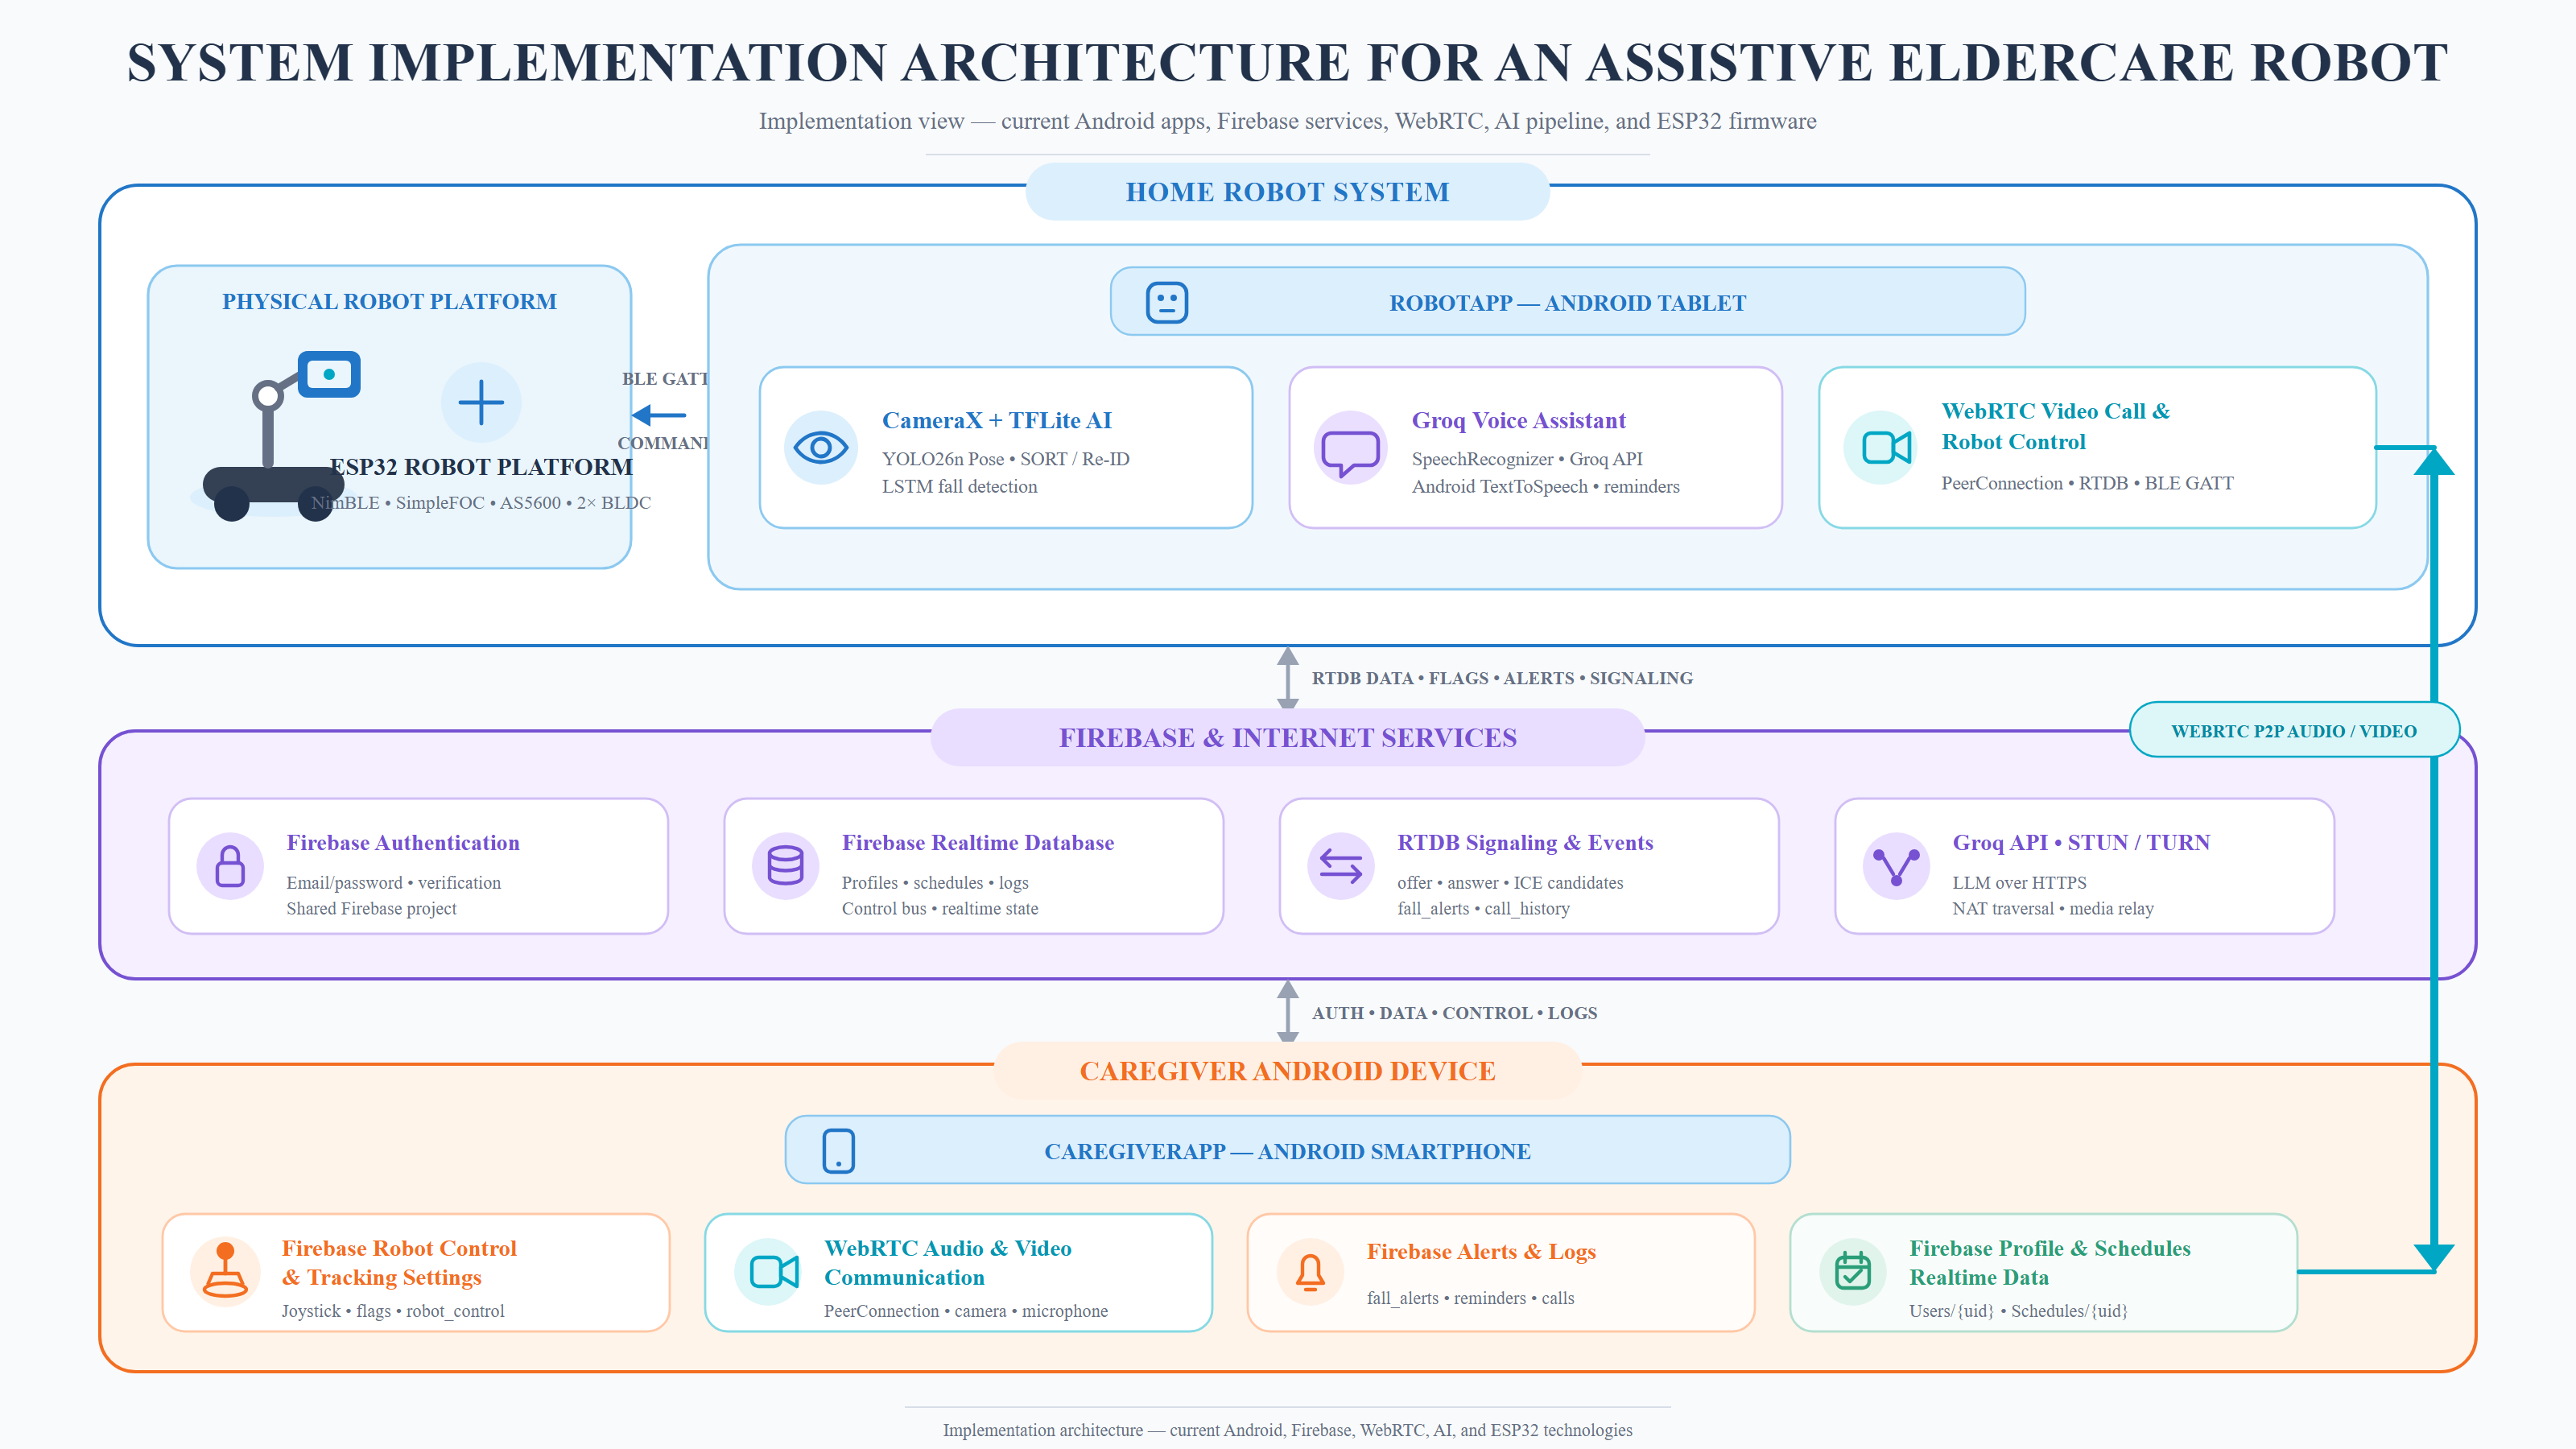
\includegraphics[width=\textwidth]{System_Implementation_Architecture_Overview_Style_Figma.png}
    \caption{Kiến trúc hiện thực của hệ thống}
    \label{fig:implementation_architecture}
\end{figure}

\subsection{Môi trường phát triển và tổ chức các thành phần}

Hệ thống gồm bốn thành phần được phát triển độc lập nhưng sử dụng cấu trúc dữ liệu và quy ước trao đổi thống nhất. RobotApp và CaregiverApp được xây dựng bằng Kotlin, giao diện XML và ViewBinding. RobotApp sử dụng package \texttt{com.example.datn\_v1}, còn CaregiverApp sử dụng package \texttt{com.example.datn\_caregiver}; cả hai cùng đặt \texttt{minSdk=23}, \texttt{targetSdk=36} và Java/Kotlin JVM target 11. Firmware được xây dựng dưới dạng chương trình Arduino cho ESP32. Thành phần AI gồm mô hình sau huấn luyện, mô hình ONNX trung gian, mô hình TFLite và các chương trình chuyển đổi, kiểm tra suy luận.

\begin{table}[htbp]
\centering
\caption{Các thành phần hiện thực của hệ thống}
\label{tab:source_blocks}
\small
\begin{tabularx}{\textwidth}{|p{3.1cm}|p{5.1cm}|X|}
\hline
\textbf{Khối} & \textbf{Công nghệ chính} & \textbf{Vai trò} \\
\hline
RobotApp & Android/Kotlin, CameraX, TFLite, OpenCV, Firebase, WebRTC, BLE, OkHttp & Xử lý AI, hội thoại, cuộc gọi và kết nối với thân robot \\
\hline
CaregiverApp & Android/Kotlin, Firebase Auth/RTDB, WebRTC & Ứng dụng cho người thân quản lý, giám sát và điều khiển \\
\hline
Mô hình AI & Python, Keras/TensorFlow, Ultralytics, ONNX, onnx2tf, TFLite & Chuẩn bị dữ liệu, huấn luyện và chuyển đổi mô hình cho Android \\
\hline
Firmware & ESP32, NimBLE, SimpleFOC, AS5600, 3PWM & Tiếp nhận, phân tích lệnh qua BLE và điều khiển hai động cơ BLDC \\
\hline
\end{tabularx}
\end{table}

RobotApp sử dụng CameraX, các gói TensorFlow Lite (CPU, GPU, Support và Select TF Ops), OpenCV Android, Firebase Authentication, Firebase Database, WebRTC native, OkHttp và Kotlin Coroutines. CaregiverApp sử dụng Firebase Authentication, Firebase Database, Android Credentials, RecyclerView và WebRTC. Tệp mô hình TFLite được cấu hình \texttt{noCompress} để giữ nguyên dạng khi đóng gói, cho phép truy cập bằng cơ chế ánh xạ tệp vào bộ nhớ.

\subsection{Hiện thực RobotApp}

\subsubsection{Khởi động, điều hướng và vòng đời dịch vụ}

\texttt{LoginActivity} là màn hình khởi động của RobotApp. Sau khi xác thực, \texttt{MainActivity} quản lý các fragment hồ sơ, theo dõi, chatbot và cuộc gọi, đồng thời lắng nghe nhánh \texttt{webrtc\_signal} để hiển thị yêu cầu gọi đến. \texttt{ReminderService} theo dõi lịch nhắc nhở; \texttt{TrackingService} duy trì thông báo của dịch vụ chạy nền và chuyển sự kiện té ngã từ khối theo dõi đến chatbot. Việc thu nhận hình ảnh và suy luận AI được thực hiện trong \texttt{tracking\_fragment}. Tệp AndroidManifest khai báo các quyền sử dụng camera, microphone, Internet, thông báo, dịch vụ nền và Bluetooth theo phiên bản hệ điều hành.

Quyền Bluetooth được khai báo theo từng nhóm phiên bản hệ điều hành. Android 11 trở xuống sử dụng \texttt{BLUETOOTH}, \path|BLUETOOTH_ADMIN| và quyền vị trí để quét thiết bị; từ Android 12, ứng dụng sử dụng \path|BLUETOOTH_SCAN| và \path|BLUETOOTH_CONNECT| theo hướng dẫn của Android \reportcite{ref:android_permissions}. Camera được khai báo \texttt{required=false} để không ngăn cài đặt chỉ vì thiết bị thiếu cờ tính năng tương ứng, nhưng các chức năng thị giác chỉ hoạt động khi có camera.

\subsubsection{TrackingFragment và quản lý camera}

\texttt{tracking\_fragment.kt} điều phối CameraX, mô hình ước lượng tư thế, bộ theo dõi, LSTM, bộ hậu kiểm và chức năng bám người. CameraX cung cấp \texttt{Preview} để hiển thị hình ảnh xem trước và \texttt{ImageAnalysis} để phân tích khung hình. Bộ phân tích chuyển dữ liệu từ \texttt{ImageProxy} sang ảnh bitmap và tensor, sau đó giải phóng khung hình đã xử lý. Hai chức năng camera được liên kết với vòng đời của fragment theo cơ chế CameraX \reportcite{ref:android_camera}.

Khi không có cuộc gọi, CameraX được gắn với vòng đời của fragment. Trước khi WebRTC khởi động, CameraX được tháo liên kết để tránh hai thành phần cùng mở camera. \texttt{video\_call\_fragment} tiếp quản camera và gửi một bản sao \texttt{VideoFrame} cục bộ về khối theo dõi. Khung hình được chuyển từ I420 sang RGB, giảm kích thước và xử lý trên một executor riêng; nếu lượt suy luận trước chưa kết thúc, khung hình mới bị bỏ qua thay vì tiếp tục xếp hàng. Khi cuộc gọi kết thúc, bộ thu hình của WebRTC được dừng và giải phóng trước khi CameraX được liên kết trở lại.

Bên cạnh việc quản lý nguồn hình ảnh, \texttt{tracking\_fragment} duy trì một đối tượng \texttt{RobotControlManager} để điều khiển kết nối với ESP32. Chức năng gọi video sử dụng chung bộ quản lý này, giúp tập trung việc kiểm tra lệnh và xử lý dừng robot.

\subsubsection{Nạp và suy luận mô hình YOLO26n-Pose}

Các quy ước về bounding box, keypoint và hậu xử lý ở Mục \ref{sec:yolo_pose_output_representation} và Mục \ref{sec:yolo_pose_inference_pipeline} được hiện thực trong \texttt{tracking\_fragment.kt}. Chuỗi xử lý bao gồm lựa chọn mô hình, khởi tạo bộ suy luận, tiền xử lý khung hình, giải mã tensor và chuyển kết quả đến SORT, LSTM cùng lớp hiển thị.

\paragraph{Mô hình triển khai và lựa chọn bộ tăng tốc.}
RobotApp đóng gói hai biến thể mô hình trong thư mục \texttt{assets}. Biến thể đầu ra thô có kích thước tensor tĩnh được ưu tiên để khai thác GPU; biến thể đầu cuối được sử dụng khi mô hình thứ nhất không thể khởi tạo. Bảng \ref{tab:yolo_runtime_artifacts} trình bày quy ước đầu ra mà bộ giải mã hỗ trợ.

\begin{table}[htbp]
\centering
\caption{Hai mô hình YOLO26n-Pose được đóng gói trong RobotApp}
\label{tab:yolo_runtime_artifacts}
\renewcommand{\arraystretch}{1.12}
\footnotesize
\begin{tabularx}{\textwidth}{|>{\raggedright\arraybackslash}p{3.55cm}|p{1.7cm}|p{2.45cm}|X|}
\hline
\textbf{Tệp mô hình} & \textbf{Kích thước} & \textbf{Đầu ra} & \textbf{Vai trò} \\
\hline
\path|yolo26n-pose_320_gpu.tflite| & 11.838.836 byte & \texttt{[1,56,2100]} & Đầu ra thô, tensor tĩnh; được ưu tiên để suy luận bằng GPU \\
\hline
\path|yolo26n-pose_320.tflite| & 12.031.560 byte & \texttt{[1,300,57]} & Đầu ra E2E; mô hình dự phòng với số lượng kết quả giới hạn \\
\hline
\end{tabularx}
\end{table}

Sau khi chọn tệp, \texttt{setupAIModel()} lần lượt thử bộ tăng tốc GPU, NNAPI và cuối cùng là CPU với bốn luồng. Nếu GPU không khởi tạo được, tài nguyên của bộ tăng tốc này được giải phóng trước khi chuyển sang NNAPI. Thay vì cố định kích thước theo tên tệp, chương trình đọc \texttt{getInputTensor(0).shape()} và \texttt{getOutputTensor(0).shape()}, sau đó cập nhật kích thước đầu vào và cấp phát bộ đệm đầu ra theo hình dạng tensor thực tế. Nhờ vậy, cùng một chuỗi xử lý có thể tiếp nhận các mô hình được xuất theo những quy ước khác nhau. TFLite được lựa chọn vì phù hợp với việc triển khai mô hình trên thiết bị di động và thiết bị biên \reportcite{ref:tflite}.

\paragraph{Tiền xử lý khung hình.}
CameraX sử dụng \texttt{STRATEGY\_KEEP\_ONLY\_LATEST} để ưu tiên khung hình mới nhất. Bộ điều phối suy luận bỏ qua khung hình khi chưa đủ khoảng thời gian cấu hình hoặc lượt xử lý trước chưa hoàn tất, nhờ đó hạn chế tích lũy ảnh cũ trong hàng đợi. Trong cuộc gọi, bản sao \texttt{VideoFrame} của WebRTC được đưa đến cùng bộ thực thi tác vụ và hàm suy luận, cho phép hai nguồn hình ảnh sử dụng chung quy trình xử lý.

Ảnh bitmap được nạp vào \texttt{TensorImage} kiểu \texttt{float32}, đổi trực tiếp về kích thước $320\times320$ bằng \texttt{ResizeOp.ResizeMethod.BILINEAR}, rồi chuẩn hóa giá trị RGB từ $[0,255]$ về $[0,1]$ bằng \texttt{NormalizeOp(0f,255f)}. Ứng dụng không thêm phần đệm ảnh theo phương pháp letterbox. Với khung hình camera $W_c\times H_c$ và $S=320$, ánh xạ từ tọa độ ảnh camera sang ảnh đầu vào mô hình là
\begin{equation}
x_i=x_c\frac{S}{W_c},\qquad y_i=y_c\frac{S}{H_c},
\end{equation}
còn phép đổi ngược là $x_c=x_iW_c/S$, $y_c=y_iH_c/S$. Hai hệ số theo hai trục được giữ riêng vì khung hình nguồn không nhất thiết là ảnh vuông.

\paragraph{Nhận dạng và giải mã cấu trúc tensor.}
Đầu ra thô chứa dự đoán tại ba mức bước lấy mẫu (stride) 8, 16 và 32. Với ảnh $320\times320$, tổng số vị trí dự đoán là
\begin{equation}
N=\left(\frac{320}{8}\right)^2+
  \left(\frac{320}{16}\right)^2+
  \left(\frac{320}{32}\right)^2=2100.
\end{equation}
Vì mô hình chỉ nhận diện lớp người, mỗi vị trí dự đoán gồm 4 giá trị hộp, 1 độ tin cậy và $17\times3$ giá trị keypoint, tổng cộng 56 kênh. Mô hình đầu ra thô trả tensor \texttt{[1,56,2100]}; hàm \texttt{getOutputVal()} xử lý sự khác biệt giữa cách sắp xếp này và dạng \texttt{[1,2100,56]}, nhờ đó bộ giải mã luôn truy cập theo cặp chỉ số dự đoán--kênh. Bốn kênh đầu biểu diễn $(c_x,c_y,w_b,h_b)$, kênh 4 là độ tin cậy, còn 51 giá trị từ kênh 5 tạo thành 17 bộ ba $(x_j,y_j,p_j)$.

Đầu ra đầu cuối (E2E) được nhận biết khi hai chiều còn lại sau chiều kích thước lô có giá trị $300$ và $57$. Mỗi hàng gồm bốn trường đầu biểu diễn $(x_{\min},y_{\min},x_{\max},y_{\max})$, trường 4 là độ tin cậy, trường 5 là nhãn lớp và các trường từ 6 chứa dữ liệu của 17 điểm khớp. Hai dạng đầu ra cần được giải mã riêng: đọc đầu ra thô theo quy ước E2E sẽ làm tọa độ tâm và kích thước bounding box bị hiểu thành tọa độ hai góc, đồng thời làm lệch vị trí các kênh điểm khớp.

Hai mô hình có thể trả tọa độ chuẩn hóa hoặc tọa độ pixel trong không gian đầu vào. Hàm \texttt{detectCoordSystem()} khảo sát kênh tọa độ ở lần suy luận đầu tiên: nếu giá trị dương lớn nhất không vượt quá 2, tọa độ được xem là đã chuẩn hóa; ngược lại, kết quả được xem là tọa độ pixel của ảnh mô hình. Trường hợp thứ nhất được nhân trực tiếp với $W_c,H_c$, còn trường hợp thứ hai được nhân với $W_c/320,H_c/320$. Quy tắc nhận biết này đáp ứng hai mô hình được sử dụng trong đề tài; khi bổ sung quy trình xuất mô hình mới, hệ tọa độ nên được khai báo rõ bằng siêu dữ liệu để tránh suy đoán.

Đầu ra thô được đổi từ dạng $cxcywh$ sang $xyxy$, sau đó loại các dự đoán có độ tin cậy dưới $0{,}20$. Hàm \texttt{nms()} sắp xếp kết quả theo điểm tin cậy và loại hộp có IoU lớn hơn $0{,}45$. Kết quả E2E cũng đi qua hàm này như một lớp lọc bổ sung, mặc dù mô hình đầu cuối đã thực hiện bước lựa chọn dự đoán. Mỗi keypoint được giữ kèm độ tin cậy và chỉ được đánh dấu \texttt{visible} khi $p_j>0{,}30$.

\paragraph{Chuyển đổi tọa độ và hiển thị kết quả.}
Quy trình xử lý sử dụng bốn hệ tọa độ như trình bày trong Bảng \ref{tab:yolo_coordinate_systems}. Bounding box và các điểm khớp phải được chuyển đổi nhất quán giữa các hệ này. Các phép tính theo dõi và điều khiển sử dụng tọa độ ảnh camera; tọa độ trên giao diện chỉ phục vụ hiển thị.

\begin{table}[htbp]
\centering
\caption{Các hệ tọa độ trong quy trình xử lý YOLO26n-Pose của RobotApp}
\label{tab:yolo_coordinate_systems}
\renewcommand{\arraystretch}{1.12}
\small
\begin{tabularx}{\textwidth}{|p{2.35cm}|p{2.35cm}|X|X|}
\hline
\textbf{Không gian} & \textbf{Miền tọa độ} & \textbf{Vai trò} & \textbf{Dữ liệu sử dụng} \\
\hline
Ảnh camera $\mathcal{C}$ & $[0,W_c]\times[0,H_c]$ pixel & Khung hình gốc nhận từ CameraX hoặc WebRTC & SORT, LSTM và điều khiển bám người \\
\hline
Ảnh mô hình $\mathcal{I}$ & $[0,320]\times[0,320]$ pixel & Ảnh vuông sau \texttt{ResizeOp} & Suy luận và đầu ra dạng pixel \\
\hline
Chuẩn hóa $\mathcal{N}$ & $[0,1]\times[0,1]$ & Biểu diễn không phụ thuộc độ phân giải & Đầu ra chuẩn hóa và các tỉ lệ hình học \\
\hline
Màn hình $\mathcal{V}$ & $[0,W_v]\times[0,H_v]$ pixel & \texttt{BoundingBoxOverlay} chồng lên preview & Vẽ hộp, skeleton, nhãn và track ID \\
\hline
\end{tabularx}
\end{table}

Camera trước được hiển thị như gương. Sau khi đổi về pixel camera, tọa độ ngang của keypoint được thay bằng $x'_c=W_c-x_c$. Với bounding box, hai cạnh phải đổi đồng thời:
\begin{equation}
x'_{\min}=W_c-x_{\max},\qquad x'_{\max}=W_c-x_{\min}.
\end{equation}
Nếu chỉ phản chiếu từng cạnh mà không hoán đổi, kết quả sẽ có cạnh phải nhỏ hơn cạnh trái. Tọa độ $y$ không thay đổi.

\texttt{BoundingBoxOverlay.onDraw()} tiếp tục ánh xạ pixel camera sang View theo center-crop giống \texttt{PreviewView}. Với
\begin{equation}
s_v=\max\!\left(\frac{W_v}{W_c},\frac{H_v}{H_c}\right),\quad
\Delta_x=\frac{W_v-s_vW_c}{2},\quad
\Delta_y=\frac{H_v-s_vH_c}{2},
\end{equation}
một điểm được vẽ tại $x_v=s_vx'_c+\Delta_x$, $y_v=s_vy_c+\Delta_y$. Phần bù có thể âm vì center-crop cắt bớt một chiều. Tọa độ View chỉ phục vụ hiển thị; các đại lượng như tâm mục tiêu, mức chiếm khung và khoảng cách keypoint vẫn được tính trong không gian camera rồi chuẩn hóa bởi $W_c,H_c$.

\paragraph{Chuyển kết quả đến các module tiếp theo.}
Sau khi giải mã, mỗi đối tượng gồm bounding box \texttt{bbox}, độ tin cậy \texttt{score}, nhãn lớp \texttt{classId} và 17 điểm khớp trước khi được chuyển đến \texttt{SortTracker}. Kết quả theo dõi được dùng để xác định mục tiêu ID0, tạo vector 69 đặc trưng cho LSTM, tính lệnh bám theo và hiển thị thông tin lên màn hình. Dữ liệu được thống nhất trong hệ tọa độ camera, nên các module phía sau không cần xử lý lại sự khác biệt về dạng đầu ra, thứ tự các chiều tensor hoặc quy ước tọa độ của từng mô hình.

\subsubsection{SORT, Kalman, Hungarian và Re-ID}

Các lớp \texttt{SortTracker}, \texttt{KalmanBoxTracker}, \texttt{HungarianAlgorithm} và \texttt{ReIdModule} hiện thực phương pháp theo dõi dựa trên kết quả phát hiện. Mỗi đối tượng gồm \texttt{bbox}, \texttt{score}, \texttt{classId} và các keypoint. Bộ lọc Kalman dự báo vùng bao ở khung hình kế tiếp, còn thuật toán Hungarian tìm phương án ghép có tổng chi phí nhỏ nhất. Phương pháp này kế thừa cấu trúc gọn của SORT \reportcite{ref:sort}, đồng thời bổ sung tín hiệu tư thế và đặc trưng ngoại hình để phù hợp hơn với bài toán trên điện thoại.

Hàm chi phí ghép đối tượng gồm bốn thành phần: 30\% sai khác IoU, 30\% khoảng cách tâm, 30\% khoảng cách giữa các điểm khớp và 10\% thay đổi diện tích bounding box. Ngưỡng IoU cơ sở của bộ theo dõi là 0,25; đối tượng mới cần hai lần ghép thành công để được xác nhận. Khi không tìm thấy kết quả phát hiện phù hợp, định danh ID0 được duy trì tối đa 45 khung hình, còn các định danh khác được giữ tối đa 10 khung hình.

Khối tái định danh trích xuất biểu đồ phân bố màu (histogram) trong không gian Hue--Saturation--Value (HSV) từ vùng thân người, nhằm giảm ảnh hưởng của hậu cảnh và thay đổi góc mặt. Đặc trưng màu không được cập nhật khi thiếu điểm khớp tin cậy, vì vùng cắt không chính xác có thể chứa hình ảnh của người khác. Khi một kết quả phát hiện phù hợp với đặc trưng đã lưu, \texttt{restoreWithId} khôi phục định danh ban đầu. Giải pháp này có chi phí tính toán thấp hơn việc bổ sung mạng trích xuất đặc trưng ngoại hình như Deep SORT \reportcite{ref:deepsort}, nhưng dễ bị ảnh hưởng khi nhiều người mặc trang phục giống nhau hoặc ánh sáng thay đổi.

\subsubsection{Duy trì mục tiêu ID0 và tạo lệnh bám theo}

Người mục tiêu được gán định danh \texttt{PRIMARY\_TRACK\_ID=0}. Việc lựa chọn ban đầu dựa trên diện tích bounding box, độ tin cậy phát hiện, tỷ lệ điểm khớp quan sát được, khoảng cách đến tâm ảnh và mức độ bị cắt ở biên. Định danh ID0 được dùng chung cho phân tích té ngã và điều khiển bám theo. Khi mất dấu, hệ thống tìm lại mục tiêu trong khoảng 2 s; đối tượng được xét phải cách vị trí cuối không quá 35\% đường chéo ảnh, nằm trong vùng trung tâm và được quan sát ổn định qua ba khung hình. Trong quá trình xử lý sự kiện nghi té ngã, hệ thống không tự chuyển sang một người khác.

Chức năng bám theo ước lượng độ gần từ kích thước bounding box và khoảng cách giữa các mốc vai, hông, gối, mắt cá chân. Giá trị sau khi làm mượt được chia thành ba vùng quá xa, phù hợp và quá gần. Ngưỡng đi vào và rời khỏi mỗi vùng khác nhau để tránh chuyển liên tục giữa tiến, dừng và lùi khi giá trị dao động gần biên. \texttt{TrackingMotionPolicy} điều chỉnh thành phần tịnh tiến theo độ gần: mức tiến tăng từ 0,60 đến 0,90, mức lùi khi mục tiêu quá gần thay đổi từ 0,45 đến 0,60, còn mức lùi để quan sát lại phần chân là 0,30. Đây là các độ lớn của lệnh điều khiển chuẩn hóa, không phải vận tốc đo bằng m/s. Khi robot vừa quay vừa tiến hoặc chưa quan sát ổn định mắt cá chân, mức tiến được giảm để hạn chế mất dấu. Sai lệch ngang giữa tâm bounding box và tâm ảnh tạo thành phần quay liên tục, có vùng chết và giới hạn biên để giảm dao động.

Một nhánh hình học riêng phân loại tư thế phục vụ điều khiển, không thay đổi kết quả FALL/NO FALL của LSTM. Nhánh này kết hợp tỷ lệ vùng bao, hướng phân bố keypoint, quan hệ vai--hông và bằng chứng từ thân dưới; \texttt{PostureGeometry} bổ sung trường hợp người nằm dọc theo hướng nhìn của camera nên hình chiếu có thể trông gần giống tư thế đứng. Khi tư thế nằm đã ổn định hoặc một sự cố té ngã đang được xử lý, robot không tiếp tục tiến mà chỉ dừng, lùi chậm hoặc quay tại chỗ để đưa người vào vùng quan sát phù hợp. Mọi vector điều khiển cuối cùng vẫn được gửi qua \texttt{RobotControlManager} để kiểm tra và chuyển thành vận tốc hai bánh.

\subsubsection{LSTM phát hiện té ngã}

\texttt{LstmFallDetector} nạp mô hình \texttt{best\_model\_lstm\_v2.tflite} có dung lượng khoảng 63,9 KB và sử dụng hai luồng CPU. Dữ liệu của mỗi đối tượng được lưu trong \texttt{FallDetectionQueue}; khi tích lũy đủ 15 khung hình, hàng đợi tạo tensor đầu vào $1\times15\times69$ kiểu số thực. Tensor đầu ra $1\times2$ biểu diễn xác suất của hai lớp hoạt động bình thường và té ngã. So với tệp Keras gốc khoảng 193,8 KB, tệp TFLite có dung lượng nhỏ hơn khi đóng gói vào ứng dụng.

Kết quả được gán nhãn FALL khi xác suất FALL lớn hơn xác suất NO FALL, sau đó chuyển đến \texttt{FallVerificationEngine} để kiểm tra bổ sung. Chỉ khi có năm kết quả FALL liên tiếp, hệ thống mới ghi nhận một chuỗi nghi té ngã. Khi bộ theo dõi khôi phục thành công ID0, hàng đợi đặc trưng vẫn được gắn với người mục tiêu. Khả năng phân tích quan hệ thời gian của LSTM \reportcite{ref:lstm} được kết hợp với bước hậu kiểm trước khi tạo cảnh báo.

\subsubsection{Hậu kiểm té ngã}

\texttt{FallVerificationEngine} tiếp nhận \texttt{FrameEvidence}, gồm trạng thái quan sát mục tiêu, vị trí tương đối của thân trên, số điểm khớp, mức độ bounding box nằm trọn trong ảnh và tỷ lệ hình dạng. Sau khi chuỗi FALL kết thúc, bộ hậu kiểm xem xét vị trí mũi, vai ở các khung hình tiếp theo. Ba khung hình liên tiếp có các điểm thân trên trong vùng 70\% phía trên ảnh sẽ loại bỏ tình huống nghi té ngã; ba khung hình liên tiếp có các điểm này nằm dưới ngưỡng, hoặc 12 khung hình liên tiếp thiếu dữ liệu quan sát, sẽ dẫn đến bước hỏi xác nhận. Khi sự kiện đã được loại bỏ hoặc xác nhận, bộ hậu kiểm chờ 10 kết quả NO FALL liên tiếp trước khi trở lại trạng thái giám sát.

Bộ hậu kiểm trả về một trong ba kết quả: chưa đủ dữ liệu để kết luận, loại bỏ tình huống nghi té ngã qua \texttt{Rejected(reason)}, hoặc yêu cầu hỏi xác nhận qua \texttt{AskForConfirmation(reason, score, evidence)}. Việc tách phần xử lý khỏi giao diện cho phép kiểm thử riêng từng trường hợp bằng chuỗi dữ liệu đầu vào mà không cần camera. Trạng thái \texttt{isIncidentActive} cho biết sự kiện đang được xử lý, còn \texttt{canAcquireNewTarget} quy định khi nào được phép chọn mục tiêu mới. Các hàm \texttt{resolveAsSafe}, \texttt{resolveAsDanger} và \texttt{reset} cập nhật kết quả xác nhận hoặc đặt lại bộ xử lý.

\begin{figure}[htbp]
    \centering
    \includegraphics[width=0.88\textwidth]{1.jpeg}
    \caption{Ví dụ khung hình té ngã trong dữ liệu tham khảo}
    \label{fig:fall_sample}
\end{figure}

\subsubsection{Luồng xác nhận và cảnh báo}

Trong mỗi sự cố, TrackingService chỉ chuyển một \texttt{FallEvent} đến chatbot. Robot dừng chuyển động, phát câu hỏi bằng TTS và lắng nghe câu trả lời trong tối đa 10 s. Những cụm từ thể hiện rõ trạng thái an toàn hoặc nguy hiểm được so khớp tại thiết bị để giảm độ trễ và hạn chế phụ thuộc vào LLM. Với câu trả lời không rõ nghĩa, hệ thống gọi mô hình phân loại theo chế độ không truyền luồng và yêu cầu kết quả có cấu trúc. Nếu người dùng xác nhận an toàn, sự cố được kết thúc tại robot; các trường hợp nguy hiểm, lỗi phân loại hoặc không có phản hồi sẽ được ghi vào \texttt{fall\_alerts}, sau đó cuộc gọi đến người chăm sóc được thực hiện khi TTS phát xong.

Bản ghi cảnh báo lưu thời điểm, trạng thái xử lý, phản hồi của người dùng và các thông tin kiểm tra bổ sung như \path|verificationReason|, \path|visibleKeypoints|, \path|bboxFullyInside| và \path|upperBodyYRatio|. Các trường này lần lượt mô tả lý do yêu cầu xác nhận, số điểm khớp quan sát được, bounding box có nằm hoàn toàn trong ảnh hay không và vị trí tương đối của phần thân trên. Chúng hỗ trợ xem lại quá trình xử lý sự kiện, nhưng chưa giải thích đầy đủ cách mô hình LSTM đưa ra dự đoán.

\subsubsection{Chatbot giọng nói}

\path|chatbot_fragment| phối hợp ba thành phần: \path|SpeechRecognizerManager| nhận dạng tiếng nói, \path|GroqChatService| xử lý hội thoại và \path|AndroidTtsService| tổng hợp tiếng nói. Giao diện hiển thị trạng thái hoạt động, biểu tượng lớn, tên robot và nội dung đang được nhận dạng hoặc phát ra. Hồ sơ tại \texttt{Users/\{uid\}} cung cấp cách xưng hô, tên người chăm sóc, tình trạng và sở thích để bổ sung ngữ cảnh cho câu trả lời.

\texttt{GroqChatService} gọi điểm cuối \texttt{/openai/v1/chat/completions} qua OkHttp. Hội thoại dạng truyền luồng sử dụng mô hình \texttt{qwen/qwen3.6-27b}, trong khi các tác vụ phân loại ngắn sử dụng \texttt{openai/gpt-oss-20b}. Lịch sử được giới hạn ở 20 thông điệp để kiểm soát độ dài ngữ cảnh. Với phản hồi theo cơ chế Server-Sent Events (SSE) có tiền tố \texttt{data:}, dịch vụ đọc nội dung tại \texttt{choices[0].delta.content}, phát từng phần qua Kotlin Flow và lưu câu trả lời hoàn chỉnh khi luồng kết thúc.

Các tác vụ liên quan đến an toàn không phụ thuộc hoàn toàn vào văn bản do LLM sinh ra. Hàm phân loại phản hồi té ngã kiểm tra trước tập từ khóa an toàn và nguy hiểm; API chỉ được gọi khi câu trả lời không rõ nghĩa, sau đó kết quả JSON được phân tích theo cấu trúc định trước. Hàm \texttt{detectCallIntent} áp dụng cách tương tự khi kết hợp từ khóa, tên hoặc quan hệ của người chăm sóc và mô hình phân loại dự phòng. Khóa API được truyền vào lớp dịch vụ và cần được cung cấp từ cấu hình bên ngoài kho mã hoặc thông qua máy chủ trung gian.

\subsubsection{Nhắc nhở theo lịch}

\texttt{ReminderService} lắng nghe lịch tại \texttt{Schedules/\{uid\}} và hồ sơ tại \texttt{Users/\{uid\}}. Khi đến thời điểm nhắc, dịch vụ tạo bản ghi dưới \texttt{reminder\_logs/\{uid\}} và gửi sự kiện đến chatbot để phát lời nhắc. Người cao tuổi có thể xác nhận, từ chối hoặc không phản hồi. Bản ghi được cập nhật trạng thái, câu trả lời, số lần nhắc lại và thời điểm xác nhận. Việc lưu riêng từng lần thực hiện cho phép người chăm sóc xem lịch sử mà không thay đổi nội dung lịch gốc.

\subsubsection{WebRTC trong RobotApp}

\texttt{video\_call\_fragment} khởi tạo \texttt{PeerConnectionFactory}, nguồn âm thanh và hình ảnh, thành phần hiển thị video cùng tham chiếu đến nhánh \texttt{webrtc\_signal}. Khi chủ động gọi, RobotApp ghi bản đề nghị \texttt{offer} và các địa chỉ ứng viên ICE vào \texttt{robotCandidates}. Khi nhận cuộc gọi, ứng dụng đọc \texttt{offer}, tạo bản trả lời \texttt{answer} và theo dõi \texttt{caregiverCandidates}. Các bộ lắng nghe được đăng ký theo từng giai đoạn thiết lập phiên và hủy khi không còn sử dụng.

WebRTC đảm nhiệm mã hóa và truyền âm thanh, hình ảnh; Firebase trao đổi SDP, ICE và trạng thái cuộc gọi \reportcite{ref:webrtc}. Trường \texttt{emergencyReason=fall} phân biệt cuộc gọi liên quan đến té ngã với cuộc gọi thông thường. Khi kết thúc, ứng dụng đặt trạng thái thành \texttt{ended}, giải phóng luồng dữ liệu, bộ thu hình, thành phần hiển thị và \texttt{PeerConnection}, sau đó trả quyền sử dụng camera cho chức năng theo dõi.

\subsubsection{RobotControlManager và BLE}

\texttt{RobotControlManager} lắng nghe nhánh \texttt{robot\_control}. Hàm ánh xạ lệnh được tách riêng để kiểm thử bằng bốn điểm chuẩn. Mỗi giá trị đầu vào được kiểm tra tính hữu hạn, giới hạn biên, độ tuổi và độ lệch thời gian về tương lai. Chuỗi lệnh được định dạng với \texttt{Locale.US} để dấu phân cách thập phân luôn là dấu chấm:

\begin{lstlisting}[caption={Định dạng lệnh BLE ở mức logic}]
left  = clamp((steering * 0.15 + translation) * 20, -20, 20)
right = clamp((steering * 0.15 - translation) * 20, -20, 20)
payload = "L%.2fR%.2f\n".format(Locale.US, left, right)
\end{lstlisting}

\texttt{RobotControlManager} tìm thiết bị theo tên \texttt{OhmniRobot} và UUID đã quy định. Thời gian quét tối đa là 10 s; khi cần khôi phục kết nối, ứng dụng thử kết nối lại sau 3 s. Sau khi tìm được dịch vụ và đặc tính nhận lệnh, ứng dụng sử dụng kiểu ghi \texttt{WRITE\_TYPE\_NO\_RESPONSE}, với cách gọi API phù hợp từng phiên bản Android. Nếu không có lệnh mới từ RTDB trong 500 ms, bộ giám sát thời gian nhận lệnh gửi lệnh dừng xuống ESP32. Hàm \texttt{stop()} cũng gửi lệnh dừng trước khi hủy các bộ lắng nghe, hàm xử lý sự kiện, tác vụ quét và kết nối GATT.

\subsection{Hiện thực CaregiverApp}

\subsubsection{Khởi động, xác thực và hồ sơ}

CaregiverApp sử dụng \texttt{LoginActivity} và \texttt{SignUpActivity} cho quá trình xác thực, \texttt{MainActivity} làm màn hình khởi động chính, còn \texttt{ProfileFragment} phục vụ quản lý hồ sơ. Firebase Authentication cung cấp UID; hồ sơ được lưu tại \texttt{Users/\{uid\}} để RobotApp cùng truy cập. \texttt{MainActivity} đồng thời khởi động \texttt{IncomingCallService} nhằm tiếp nhận cuộc gọi khi ứng dụng chạy nền. Do Activity này được khai báo là launcher, bước kiểm tra phiên xác thực ngay khi khởi động cần được hoàn thiện trước khi triển khai cho người dùng thực tế.

\subsubsection{Bật/tắt chức năng theo dõi}

\path|tracking_fragment| cập nhật hai giá trị trạng thái \path|robot_follow_enabled| và \path|ai_fall_detection_enabled| để bật, tắt các chức năng tương ứng. Fragment theo dõi \texttt{.info/connected} để hiển thị tình trạng kết nối RTDB. Khi tắt bám theo tự động, CaregiverApp đồng thời gửi lệnh $x=0,y=0$ kèm thời điểm hiện tại để robot dừng chuyển động.

\subsubsection{Lịch và nhật ký}

Danh sách lịch tại \path|Schedules/uid| được đọc bởi \texttt{ScheduleFragment}. Người chăm sóc tạo hoặc cập nhật lịch qua \texttt{AddScheduleFragment}; \texttt{ScheduleAdapter} hiển thị danh sách bằng RecyclerView và liên kết công tắc bật, tắt với trường \texttt{active}. Nhật ký lời nhắc, cảnh báo té ngã và cuộc gọi có các fragment cùng bộ hiển thị danh sách riêng. Cảnh báo và cuộc gọi được truy vấn theo thời điểm trong bảy ngày gần nhất.

\subsubsection{Tiếp nhận cuộc gọi khi ứng dụng chạy nền}

\texttt{IncomingCallService} là dịch vụ chạy nền có thông báo thường trực (foreground service), lắng nghe nhánh \texttt{webrtc\_signal}. Khi nhận \texttt{status=calling} và \texttt{callerRole=robot}, dịch vụ tạo thông báo và có thể mở \texttt{IncomingCallActivity} toàn màn hình. Nếu có \texttt{emergencyReason=fall}, nội dung thông báo cho biết cuộc gọi được tạo sau tình huống chưa xác nhận an toàn. Tệp Manifest khai báo các quyền liên quan đến thông báo, dịch vụ nền và hiển thị toàn màn hình; khả năng hiển thị phụ thuộc vào quyền được cấp và chính sách của hệ điều hành.

\subsubsection{Gọi video và điều khiển robot từ xa}

\texttt{video\_call\_fragment} xử lý cả vai trò gọi đi và nhận cuộc gọi, hiển thị hình ảnh cục bộ, từ xa và trao đổi thông tin thiết lập phiên. Trong màn hình gọi, cần điều khiển ảo tính $x=\Delta y/r$, $y=-\Delta x/r$, giới hạn giá trị trong $[-1,1]$ và giới hạn tần suất gửi lệnh khoảng 20 Hz. Khi người dùng bắt đầu điều khiển, ứng dụng tắt bám theo tự động để tránh hai nguồn lệnh cùng hoạt động. Các sự kiện \texttt{ACTION\_UP}, \texttt{ACTION\_CANCEL}, kết thúc cuộc gọi và rời màn hình đều gửi lệnh dừng.

CaregiverApp gửi lệnh điều khiển chuẩn hóa qua Internet. RobotApp tiếp nhận, kiểm tra và chuyển lệnh thành vận tốc của hai động cơ theo quy ước lắp đặt, rồi truyền đến ESP32 qua BLE. Nhờ đó, người chăm sóc có thể điều khiển từ xa khi hai ứng dụng có kết nối Internet, còn việc giao tiếp với phần thân được thực hiện tại robot.

\subsection{Hiện thực dữ liệu dùng chung}

Các bộ lắng nghe Firebase cung cấp bản cập nhật gần thời gian thực, trong khi thao tác ghi có thể được phản ánh cục bộ trước khi đồng bộ với máy chủ \reportcite{ref:firebase_rtdb}. Vì vậy, mỗi lệnh điều khiển bắt buộc phải có timestamp; callback được gọi theo thời gian thực không có nghĩa dữ liệu nhận được luôn còn hiệu lực. Các lớp \texttt{UserProfile}, \texttt{ScheduleItem}, \texttt{FallAlertEntry}, \texttt{ReminderLogEntry} và \texttt{CallHistoryEntry} được dùng để ánh xạ dữ liệu JSON sang đối tượng trong ứng dụng.

Hồ sơ, lịch và nhật ký lời nhắc được lưu dưới các nhánh cấp gốc nhưng đều tiếp tục phân vùng theo UID. Các kênh vận hành gồm cờ chức năng, lệnh điều khiển, signaling, cảnh báo té ngã và lịch sử cuộc gọi được tập trung dưới \texttt{pair\_sessions/\{uid\}}. Security Rules áp dụng nguyên tắc từ chối mặc định và chỉ cho phép tài khoản đã xác thực truy cập nhánh có UID tương ứng \reportcite{ref:firebase_security}. Cấu trúc này ngăn dữ liệu của các tài khoản khác nhau dùng chung kênh vận hành, nhưng hai thiết bị trong một cặp vẫn đăng nhập bằng cùng tài khoản nên chưa biểu diễn được vai trò robot và người chăm sóc như hai danh tính độc lập.

\subsection{Huấn luyện và chuyển đổi mô hình AI}

Mô hình phát hiện té ngã được chuẩn bị theo một quy trình liên tục từ xử lý dữ liệu video, trích xuất đặc trưng tư thế, huấn luyện LSTM đến chuyển đổi sang định dạng phù hợp với Android. Việc thống nhất quy ước đặc trưng giữa giai đoạn huấn luyện và suy luận có ý nghĩa quyết định, bởi chỉ một sai khác về thứ tự hoặc cách chuẩn hóa tọa độ cũng làm đầu vào trên thiết bị không còn tương thích với mô hình.

\subsubsection{Xử lý dữ liệu}

Dữ liệu LE2I được cung cấp dưới dạng các video liên tục gồm hoạt động bình thường và tình huống té ngã. Quá trình tiền xử lý gồm:
\begin{itemize}
    \item \textbf{Trích xuất khung hình}: Video được phân tách thành các khung hình ở tốc độ 25 FPS để tương thích với tốc độ xử lý mục tiêu của camera robot.
    \item \textbf{Phân chia tập dữ liệu}: Tập huấn luyện, xác thực và kiểm tra được chia theo video và chủ thể, không chia ngẫu nhiên theo từng khung hình. Cách tổ chức này hạn chế rò rỉ dữ liệu khi những khung hình gần nhau của cùng một hành động xuất hiện đồng thời ở tập huấn luyện và tập kiểm tra.
    \item \textbf{Xử lý mất cân bằng lớp}: Số mẫu hoạt động bình thường thường lớn hơn số mẫu té ngã. Trọng số lớp và phương pháp lấy mẫu tăng cường được sử dụng để giảm xu hướng mô hình nghiêng về lớp NO FALL.
\end{itemize}

\subsubsection{Trích xuất đặc trưng}

Mô hình LSTM không nhận trực tiếp ảnh RGB mà học từ chuỗi đặc trưng tư thế do YOLO-Pose cung cấp. Mỗi khung hình của người mục tiêu được biểu diễn bởi 69 giá trị theo đúng quy ước sử dụng trong RobotApp:
\begin{enumerate}
    \item \textbf{Tọa độ chuẩn hóa}: Tọa độ $(x_i,y_i)$ của 17 keypoint được chuẩn hóa theo tâm hông và kích thước của vùng tư thế, giúp giảm ảnh hưởng của vị trí và khoảng cách giữa người với camera.
    \item \textbf{Đặc trưng chuyển động}: Với mỗi keypoint, hai thành phần $(\Delta x_i,\Delta y_i)$ biểu diễn độ dịch chuyển so với khung hình trước. Mỗi điểm vì vậy đóng góp bốn giá trị $(x_i,y_i,\Delta x_i,\Delta y_i)$.
    \item \textbf{Tỷ lệ hình dạng và cửa sổ thời gian}: Tỷ lệ rộng/cao của bounding box được ghép với 68 giá trị keypoint để tạo vector 69 chiều. Mười lăm khung hình liên tiếp hình thành tensor đầu vào có kích thước $[1,15,69]$ cho LSTM.
\end{enumerate}

Cấu trúc tế bào LSTM đã được giới thiệu ở Hình \ref{fig:lstm_architecture}. Trong ứng dụng, chuỗi đặc trưng tư thế được đưa vào mô hình để phân tích sự thay đổi chuyển động theo thời gian.






\subsubsection{Huấn luyện mô hình}

Mô hình LSTM được xây dựng bằng TensorFlow/Keras. Quá trình huấn luyện gồm:
\begin{itemize}
    \item Thiết lập seed cố định để tăng khả năng tái lập thí nghiệm.
    \item Sử dụng hàm mất mát Binary Cross-Entropy cho bài toán phân loại nhị phân.
    \item Áp dụng dừng sớm khi hàm mất mát trên tập xác thực không còn cải thiện, đồng thời lưu mô hình tốt nhất tại \texttt{best\_model\_lstm.h5}.
\end{itemize}

\subsubsection{Chuyển đổi và tối ưu mô hình}

Để triển khai trên điện thoại Android, mô hình sau huấn luyện được chuyển sang TensorFlow Lite nhằm giảm kích thước và tận dụng môi trường suy luận dành cho thiết bị biên.

\textbf{1. Đối với mô hình LSTM:} \\
Chương trình \path|convert_to_tflite.py| nạp \texttt{best\_model\_lstm.h5} và kiểm tra \texttt{input\_shape} trước khi chuyển đổi bằng \path|TFLiteConverter.from_keras_model|. Tập toán tử gồm TFLite built-ins và Select TF Ops. Kết quả là \texttt{best\_model\_lstm\_v2.tflite}, có thể đóng gói trực tiếp trong thư mục \texttt{assets} của RobotApp.

\textbf{2. Đối với mô hình YOLO-Pose:} \\
Mô hình PyTorch \texttt{yolo26n-pose.pt} trước hết được xuất sang ONNX với kích thước lô cố định bằng 1 và ảnh đầu vào $320\times320$. Thư viện \texttt{onnx2tf} tiếp tục chuyển mô hình ONNX sang SavedModel và TFLite. Biến thể FP16 lưu trọng số bằng số dấu phẩy động 16 bit, qua đó giảm dung lượng và băng thông bộ nhớ so với FP32; mức ảnh hưởng đến chất lượng cần được xác nhận bằng phép kiểm tra tương đương sau chuyển đổi.

\begin{table}[htbp]
\centering
\caption{Các mô hình chính sau khi huấn luyện và chuyển đổi}
\label{tab:model_artifacts}
\small
\begin{tabularx}{\textwidth}{|p{4.3cm}|p{2.5cm}|p{2.2cm}|X|}
\hline
\textbf{Tệp mô hình} & \textbf{Định dạng} & \textbf{Dung lượng} & \textbf{Mục đích} \\
\hline
best\_model\_lstm.h5 & Keras H5 & 193,8 KB & Mô hình gốc để huấn luyện và đánh giá \\
\hline
best\_model\_lstm\_v2.tflite & TFLite & 63,9 KB & Mô hình LSTM đã tối ưu cho Android \\
\hline
yolo26n-pose.pt & PyTorch & 7,88 MB & Mô hình Pose gốc \\
\hline
yolo26n-pose\_320\_fp16.tflite & TFLite FP16 & 6,28 MB & Biến thể YOLO đã lượng tử hóa FP16, tối ưu kích thước và tốc độ \\
\hline
\end{tabularx}
\end{table}

\subsubsection{Quy trình kiểm tra tương đương sau chuyển đổi}
Quy trình kiểm tra tương đương sử dụng cùng một tập dữ liệu đầu vào cho mô hình gốc và mô hình TFLite, sau đó đối chiếu bounding box, độ tin cậy, điểm khớp và vector xác suất của LSTM. Các phép so sánh nhằm phát hiện sai khác về toán tử, thứ tự đầu ra hoặc cách chuẩn hóa mà việc nạp mô hình thành công chưa phản ánh được. Đây là bước cần hoàn thiện cùng với lưu trữ dữ liệu đầu vào và kết quả so sánh để đánh giá đầy đủ ảnh hưởng của quá trình chuyển đổi.


\subsection{Hiện thực firmware phần thân robot}

\subsubsection{Khởi tạo phần cứng}

Firmware sử dụng ESP32 để giao tiếp với hai cảm biến góc AS5600 qua hai bus I2C. Cảm biến của động cơ trái nối với SDA=19/SCL=18, còn cảm biến của động cơ phải nối với SDA=23/SCL=5. Mạch công suất bên trái dùng IN1=32, IN2=33, IN3=25, EN=22; bên phải dùng IN1=26, IN2=27, IN3=14, EN=12. Hai bus I2C riêng cho phép sử dụng đồng thời hai AS5600 có cùng địa chỉ mặc định.

Hai đối tượng \texttt{BLDCMotor} được cấu hình với 7 cặp cực và liên kết với cảm biến góc cùng mạch công suất điều khiển bằng ba tín hiệu PWM. Chương trình thiết lập phương pháp điều chế \texttt{SpaceVectorPWM}, chế độ điều khiển vận tốc \texttt{velocity}, các tham số PID và bộ lọc thông thấp trước khi gọi \texttt{init()} và \texttt{initFOC()}. Trong vòng lặp chính, \texttt{loopFOC()} được gọi liên tục, không chèn thời gian chờ bằng \texttt{delay()}.

\subsubsection{Tiếp nhận lệnh qua BLE GATT}

NimBLE khởi tạo thiết bị có tên \texttt{OhmniRobot}, thiết lập công suất phát và đưa UUID dịch vụ vào dữ liệu phản hồi quét để hỗ trợ tìm kiếm. Đặc tính nhận lệnh sử dụng thuộc tính ghi không phản hồi \texttt{WRITE\_NR}. Khi kết nối được thiết lập, hàm xử lý sự kiện cập nhật trạng thái và tiếp tục phát quảng bá; khi ngắt kết nối, vận tốc đặt của hai bánh được đưa về 0. Khi nhận dữ liệu ghi, chương trình lấy chuỗi \texttt{std::string}, loại khoảng trắng ở đầu và cuối, rồi chuyển sang bộ phân tích lệnh.

Bộ phân tích tìm vị trí hai ký tự L và R, tách chuỗi con rồi chuyển sang số bằng \texttt{toFloat}. Khi dữ liệu hợp lệ, vận tốc đặt và \texttt{lastCmdTime} được cập nhật. RobotApp đã chuẩn hóa định dạng lệnh trước khi gửi; tuy nhiên, firmware vẫn cần kiểm tra toàn bộ chuỗi và dùng \texttt{isfinite} để loại giá trị không hợp lệ ngay tại tầng chấp hành.

\subsubsection{Xử lý vùng không đáp ứng và dừng khi mất lệnh}

Hàm \texttt{applyDeadzone} đưa $|v|<0,5$ về 0, nâng độ lớn của lệnh khác 0 nhưng nhỏ hơn 3 lên 3, rồi giới hạn kết quả trong $[-40,40]$. Cơ chế watchdog theo dõi thời gian kể từ lần nhận lệnh gần nhất khi BLE đang kết nối. Nếu thời gian này vượt 800 ms và vận tốc đặt khác 0, firmware ghi nhật ký và đưa vận tốc đặt của cả hai bánh về 0. Do \texttt{motor.move()} được gọi sau bước kiểm tra, lệnh dừng được áp dụng ngay trong chu kỳ điều khiển hiện tại.

\begin{lstlisting}[caption={Giả mã xử lý lệnh và điều khiển động cơ trên ESP32}]
loopFOC(left); loopFOC(right)
if connected and now - lastCommand > 800 ms:
    targetLeft = 0; targetRight = 0
leftCommand  = applyDeadzone(targetLeft)
rightCommand = applyDeadzone(targetRight)
move(leftCommand); move(rightCommand)
\end{lstlisting}

\subsection{Kết luận chương}

Chương đã trình bày quá trình hiện thực kiến trúc hệ thống thành hai ứng dụng Android, các mô hình AI và firmware ESP32. RobotApp đảm nhiệm cảm nhận, hội thoại, điều phối và kết nối với thân robot; CaregiverApp cung cấp các chức năng quản lý, giám sát và can thiệp từ xa. Firebase, WebRTC và BLE tạo thành ba kênh giao tiếp tương ứng cho dữ liệu dùng chung, truyền thông đa phương tiện và điều khiển phần cứng. Bên cạnh đó, quy trình chuyển đổi mô hình và các cơ chế dừng nhiều tầng giúp hệ thống phù hợp hơn với điều kiện vận hành trên thiết bị di động. Chương 5 tiến hành kiểm thử, đánh giá kết quả và phân tích những giới hạn của hệ thống.

\clearpage
\section{Kết quả và thảo luận}

\subsection{Mục tiêu đánh giá}

Đánh giá nguyên mẫu nhằm trả lời bốn câu hỏi: các khối có được hiện thực đúng kiến trúc hay không; quy ước trao đổi dữ liệu giữa các ứng dụng có nhất quán hay không; các cơ chế an toàn có điểm kiểm chứng hay không; và bằng chứng hiện có cho phép kết luận tới mức nào. Do hệ thống gồm AI, cloud, mobile và phần cứng, một con số accuracy đơn lẻ không đại diện cho toàn hệ thống.

Chương này phân biệt ba loại bằng chứng. \textit{Bằng chứng tĩnh} được rút từ mã nguồn, cấu hình và artifact. \textit{Bằng chứng tự động} đến từ unit test/build có thể chạy lặp. \textit{Bằng chứng tích hợp} đến từ thử nghiệm hai điện thoại, Internet, BLE và robot thật. Chỉ các kết quả có artifact hoặc được nhóm dự án xác nhận mới được ghi ``đạt''; hạng mục thiếu log định lượng được ghi rõ để tránh tạo số liệu.

\subsection{Cấu hình và tiêu chí đánh giá}
\label{subsec:eval_criteria}

\begin{table}[htbp]
\centering
\caption{Cấu hình phần mềm được đánh giá}
\label{tab:evaluation_config}
\small
\begin{tabularx}{\textwidth}{|p{4.2cm}|X|}
\hline
\textbf{Hạng mục} & \textbf{Cấu hình} \\
\hline
RobotApp & Android/Kotlin; minSdk 23; target/compile SDK 36; CameraX; TFLite; OpenCV; Firebase; WebRTC; BLE \\
\hline
CaregiverApp & Android/Kotlin; minSdk 23; target/compile SDK 36; Firebase; WebRTC \\
\hline
AI trên Android & Pose input 320$\times$320; LSTM input $15\times69$; CPU/GPU TFLite artifacts \\
\hline
Firmware & ESP32; NimBLE; SimpleFOC; hai AS5600; hai BLDC; velocity limit 40 rad/s \\
\hline
Cloud & Firebase Authentication/RTDB; Groq HTTPS; STUN/TURN cho WebRTC \\
\hline
Giao thức điều khiển & RTDB $x,y,ts$; BLE \texttt{L<float>R<float>\textbackslash n} \\
\hline
\end{tabularx}
\end{table}

Các chỉ số AI thích hợp gồm precision, recall, F1 và confusion matrix ở cấp sự cố. Với $TP$ là phát hiện đúng sự cố, $FP$ là cảnh báo giả, $FN$ là bỏ sót:

\begin{align}
Precision &= \frac{TP}{TP+FP},\\
Recall &= \frac{TP}{TP+FN},\\
F_1 &= 2\frac{Precision\cdot Recall}{Precision+Recall}.
\end{align}

Đơn vị đánh giá phải là một sự kiện té ngã, không phải từng frame; nhiều frame cảnh báo liên tiếp của cùng sự cố chỉ tính một sự kiện. Với tracking, chỉ số cần theo dõi là số lần ID0 đổi sai, tỷ lệ phục hồi đúng và thời gian mất mục tiêu. Với điều khiển, chỉ số là độ trễ end-to-end, tần số lệnh, tỷ lệ lệnh bị loại và thời gian dừng sau mất kênh. Với WebRTC, chỉ số gồm thời gian thiết lập, tỷ lệ cuộc gọi thành công, RTT, jitter và packet loss từ \texttt{getStats}.

\subsection{Kết quả hiện thực và artifact}

\subsubsection{Mức độ hoàn thành thành phần}

\begin{longtable}{|p{4.0cm}|p{2.3cm}|p{6.7cm}|}
\caption{Kết quả hiện thực theo thành phần}\label{tab:implementation_results}\\
\hline
\textbf{Thành phần} & \textbf{Trạng thái} & \textbf{Bằng chứng} \\
\hline
\endfirsthead
\hline
\textbf{Thành phần} & \textbf{Trạng thái} & \textbf{Bằng chứng} \\
\hline
RobotApp Android & Đã hiện thực & 28 tệp Kotlin; manifest; tài nguyên giao diện và ba mô hình trong assets \\
\hline
CaregiverApp Android & Đã hiện thực & 25 tệp Kotlin; giao diện quản lý, nhật ký, lịch nhắc nhở và cuộc gọi \\
\hline
Pose trên thiết bị & Đã tích hợp & Hai model TFLite CPU/GPU và pipeline decode/NMS \\
\hline
Tracking và Re-ID & Đã tích hợp & SORT, Kalman, Hungarian, HSV histogram, ID0 \\
\hline
LSTM và hậu kiểm & Đã tích hợp & Model TFLite, queue 15$\times$69, state machine, verification engine \\
\hline
Hội thoại giọng nói & Đã tích hợp RobotApp & SpeechRecognizer, Groq streaming/classify, Android TTS \\
\hline
Lịch nhắc nhở và nhật ký & Đã tích hợp & Schedules, reminder\_logs, adapters và service \\
\hline
WebRTC & Đã tích hợp & Caller/callee, SDP/ICE RTDB, incoming foreground service \\
\hline
Điều khiển robot & Đã tích hợp & Joystick, RTDB, RobotControlManager, BLE GATT \\
\hline
Firmware BLDC & Đã hiện thực & Sketch ESP32, NimBLE, SimpleFOC, dual I2C, watchdog \\
\hline
Backend riêng/MQTT & Không thuộc hiện thực & Hệ thống dùng Firebase RTDB; không có broker/server signaling riêng \\
\hline
Chatbot CaregiverApp & Placeholder & Logic hội thoại thật chỉ nằm ở RobotApp \\
\hline
\end{longtable}

\subsubsection{Kết quả đóng gói Android}

Nhóm dự án xác nhận cả hai ứng dụng build thành công. Trong cây build có APK debug RobotApp khoảng 504,24 MiB và CaregiverApp khoảng 51,03 MiB. Chênh lệch chủ yếu do RobotApp đóng gói nhiều runtime native và thư viện AI (TFLite, GPU/Select TF Ops, OpenCV, WebRTC) cùng model; CaregiverApp không chứa model pose/LSTM và stack AI.

Kích thước 504 MiB là chấp nhận được cho prototype debug nhưng không phù hợp phát hành. Bản release cần bật shrinking, loại ABI không dùng, kiểm tra trùng native library, cân nhắc Play App Bundle/split APK và bỏ dependency AI dư. Model thực chỉ chiếm khoảng vài chục MB; phần lớn dung lượng tăng đến từ runtime/native binaries và ký hiệu debug.

\begin{table}[htbp]
\centering
\caption{Artifact đóng gói hiện có}
\label{tab:apk_results}
\begin{tabular}{|l|r|l|}
\hline
\textbf{Artifact} & \textbf{Kích thước} & \textbf{Ý nghĩa} \\
\hline
RobotApp debug APK & 504,24 MiB & Bản debug tích hợp AI/WebRTC/BLE \\
\hline
CaregiverApp debug APK & 51,03 MiB & Bản debug quản lý/WebRTC \\
\hline
\end{tabular}
\end{table}

\subsubsection{Kết quả artifact mô hình}

Chuỗi chuyển đổi đã tạo đủ artifact H5, PT, ONNX, SavedModel và TFLite. LSTM giảm từ khoảng 189,2 KB ở dạng Keras xuống 59,6 KB ở dạng TFLite không lượng tử hóa. Biến thể pose FP16 trong cây chuyển đổi có dung lượng 6,01 MB, khoảng một nửa biến thể float32 tương ứng là 11,87 MB; hai biến thể được đóng gói trong ứng dụng có dung lượng lần lượt khoảng 12,03 MB và 11,84 MB. Đây là kết quả về kích thước tệp, không tự động chứng minh tốc độ hoặc độ chính xác.

\begin{table}[htbp]
\centering
\caption{Đánh giá định tính các biến thể mô hình}
\label{tab:model_variant_discussion}
\small
\begin{tabularx}{\textwidth}{|p{3.2cm}|p{3.3cm}|X|}
\hline
\textbf{Biến thể} & \textbf{Lợi ích kỳ vọng} & \textbf{Điều phải đo} \\
\hline
Float32 CPU & Tương thích rộng, dễ debug & Latency, nhiệt, FPS, bộ nhớ \\
\hline
Graph GPU & Tăng throughput nếu delegate hỗ trợ toàn graph & Tỷ lệ op chạy GPU, overhead copy, fallback \\
\hline
FP16 & Giảm dung lượng/băng thông bộ nhớ & Sai số keypoint, mAP/PCK, latency thật \\
\hline
NMS ngoài graph & Tăng tính tương thích delegate & Độ đúng decode/NMS Kotlin so với nguồn \\
\hline
\end{tabularx}
\end{table}

\subsection{Kiểm thử tự động ở mức logic}

Các lớp xử lý độc lập với giao diện được kiểm thử bằng JUnit để có thể tái hiện các điều kiện biên mà không cần camera hoặc robot thật. Phiên bản hiện tại có 24 phương thức kiểm thử trực tiếp cho logic của đề tài, phân bố ở các nhóm đường dẫn Firebase, ánh xạ lệnh động cơ, chính sách bám người, hình học tư thế và hậu kiểm té ngã. Hai kiểm thử mẫu do Android Studio tạo sẵn không được tính vào nhóm này.

\subsubsection{Ánh xạ lệnh và chính sách bám người}

\texttt{RobotControlManagerTest} gồm sáu trường hợp bảo vệ quy ước dấu và hệ số chuyển đổi từ vector $(x,y)$ sang vận tốc hai bánh. Bốn trường hợp đầu kiểm tra tiến, lùi và quay tại chỗ; hai trường hợp còn lại xác nhận nhiễu quay nhỏ bị loại khi robot đang tịnh tiến mạnh, trong khi lệnh quay đủ lớn vẫn được giữ lại. Các phép so sánh sử dụng sai số $0,001$.

\begin{table}[htbp]
\centering
\caption{Các trường hợp kiểm thử ánh xạ điều khiển}
\label{tab:control_unit_tests}
\small
\begin{tabularx}{\textwidth}{|p{4.5cm}|p{3.2cm}|X|}
\hline
\textbf{Nhóm kiểm thử} & \textbf{Đầu vào tiêu biểu} & \textbf{Kết quả mong đợi} \\
\hline
Tiến và lùi theo hiệu chỉnh & $(-1,0)$; $(1,0)$ & $(-20,20)$; $(20,-20)$ \\
\hline
Quay tại chỗ & $(0,1)$; $(0,-1)$ & $(3,3)$; $(-3,-3)$ \\
\hline
Loại nhiễu quay nhỏ & $(0{,}4;\,0{,}2)$ & $(8,-8)$, thành phần quay nhỏ bị loại \\
\hline
Duy trì lệnh quay có chủ đích & $(0{,}4;\,0{,}5)$ & $(9{,}5;-6{,}5)$ \\
\hline
\end{tabularx}
\end{table}

\texttt{TrackingMotionPolicyTest} bổ sung bốn trường hợp cho chính sách vận tốc. Các kiểm thử xác nhận tốc độ tiến tăng theo độ xa nhưng không vượt giới hạn, tốc độ được giảm khi robot đang quay hoặc chưa quan sát ổn định mắt cá chân, tốc độ lùi tăng khi người ở quá gần, và thành phần hiệu chỉnh hướng nhỏ vẫn vượt được vùng không đáp ứng của động cơ khi robot đang tịnh tiến. Nhóm kiểm thử này phản ánh thay đổi từ các lệnh rời rạc sang vector chuyển động biến thiên theo khoảng cách.

\subsubsection{Hậu kiểm té ngã và hình học tư thế}

\texttt{FallVerificationEngineTest} gồm sáu trường hợp kiểm tra trực tiếp chuỗi trạng thái của bộ hậu kiểm. Một kết quả FALL đơn lẻ không được mở sự cố; chỉ năm kết quả FALL liên tiếp mới tạo ứng viên, và một kết quả NO FALL xen giữa phải xóa bộ đếm ứng viên. Sau khi chuỗi FALL kết thúc, ba khung hình có điểm thân trên trong 70\% phía trên ảnh làm ứng viên bị loại; ba khung hình có điểm thân trên thấp hơn ngưỡng hoặc 12 khung hình liên tiếp không còn bằng chứng quan sát sẽ dẫn đến yêu cầu xác nhận.

\begin{table}[htbp]
\centering
\caption{Các trường hợp kiểm thử hậu kiểm té ngã}
\label{tab:fall_unit_tests}
\small
\begin{tabularx}{\textwidth}{|p{4.4cm}|X|p{3.2cm}|}
\hline
\textbf{Trường hợp} & \textbf{Chuỗi đầu vào} & \textbf{Kết quả mong đợi} \\
\hline
Nhiễu FALL đơn lẻ & Một kết quả FALL & Chưa mở sự cố \\
\hline
Chuỗi FALL ổn định & Năm FALL liên tiếp, sau đó ba khung hình thân trên ở cao & Hình thành ứng viên rồi loại sau hậu kiểm \\
\hline
Chuỗi ứng viên bị gián đoạn & Bốn FALL, một NO FALL, sau đó bốn FALL & Bộ đếm được đặt lại, chưa mở sự cố \\
\hline
Thân trên còn ở vùng cao & Ba khung hình có $y/H\leq0,70$ sau chuỗi FALL & Loại ứng viên \\
\hline
Thân trên ở vùng thấp & Ba khung hình có $y/H>0,70$ sau chuỗi FALL & Yêu cầu xác nhận \\
\hline
Mất mục tiêu sau chuỗi FALL & 12 khung hình không có bằng chứng thân trên & Yêu cầu xác nhận \\
\hline
\end{tabularx}
\end{table}

\texttt{PostureGeometryTest} có bốn trường hợp được xây dựng từ các mẫu tư thế đứng, nằm, đang đứng dậy và thiếu keypoint thân dưới. Mục đích của nhóm này là kiểm tra riêng cách nhận biết tư thế nằm bị co ngắn theo phối cảnh camera. Kết quả chỉ được dùng để lựa chọn hành vi chuyển động an toàn, không thay thế nhãn FALL/NO FALL của LSTM.

\subsubsection{Phân vùng đường dẫn Firebase}

Hai ứng dụng đều có \texttt{FirebasePairPathsTest} với cùng hai nguyên tắc kiểm tra. Các UID khác nhau phải tạo ra những đường dẫn điều khiển, cuộc gọi và cảnh báo khác nhau; toàn bộ kênh vận hành của một cặp thiết bị phải nằm dưới \texttt{pair\_sessions/\{uid\}}. Việc duy trì cùng bộ kiểm thử ở RobotApp và CaregiverApp giúp phát hiện sớm sai lệch đường dẫn khi một trong hai ứng dụng thay đổi cấu trúc dữ liệu.

\subsection{Đánh giá tính nhất quán khi tích hợp bằng kiểm tra tĩnh}

\subsubsection{Nhất quán Firebase}

Đối chiếu hai ứng dụng cho thấy các đường dẫn vận hành được tạo thống nhất bởi \texttt{FirebasePairPaths}: \path|robot_control|, \path|robot_follow_enabled|, \path|ai_fall_detection_enabled|, \path|webrtc_signal|, \path|fall_alerts| và \path|call_history| đều là nhánh con của \texttt{pair\_sessions/\{uid\}}. Hồ sơ, lịch và nhật ký lời nhắc lần lượt nằm dưới \texttt{Users/\{uid\}}, \texttt{Schedules/\{uid\}} và \texttt{reminder\_logs/\{uid\}}. Offer/answer dùng cùng các trường \texttt{sdp,type}; ICE dùng \path|candidate,sdpMid,sdpMLineIndex| và được tách nhánh theo vai trò.

Security Rules từ chối truy cập ở cấp gốc và chỉ mở từng nhánh khi UID xác thực trùng với UID trên đường dẫn. Cách tổ chức hiện tại vì vậy đã cách ly dữ liệu giữa các tài khoản. Giới hạn còn lại là RobotApp và CaregiverApp trong một cặp dùng chung tài khoản, nên hệ thống chưa phân biệt quyền của hai thiết bị hoặc biểu diễn quan hệ nhiều người chăm sóc--nhiều robot.

\subsubsection{Nhất quán BLE}

Tên thiết bị, UUID của service và characteristic trong \texttt{RobotControlManager} trùng với firmware. RobotApp tạo chuỗi gồm giá trị bánh trái đứng trước bánh phải, sử dụng dấu chấm thập phân và kết thúc bằng ký tự xuống dòng; firmware loại khoảng trắng rồi tách hai giá trị tại ký tự L và R. RobotApp giới hạn vận tốc trong $[-20,20]$ rad/s, hẹp hơn giới hạn $[-40,40]$ rad/s của firmware. Characteristic ở hai phía đều sử dụng chế độ ghi không phản hồi.

\subsubsection{Chuỗi timeout}

Ba mốc thời gian tạo thành các lớp bảo vệ kế tiếp: RobotApp gửi lệnh dừng sau 500 ms không nhận cập nhật từ RTDB, firmware đưa vận tốc đặt về 0 sau 800 ms không nhận payload BLE, còn lệnh RTDB có tuổi lớn hơn 2.000 ms trên mốc thời gian đã đồng bộ bị loại khi ứng dụng nhận dữ liệu. Với joystick cập nhật khoảng 20 Hz, chu kỳ lệnh danh định là 50 ms, nhỏ hơn đáng kể so với hai mốc dừng. RobotApp vì vậy chủ động dừng trước, trong khi firmware đóng vai trò bảo vệ cuối cùng nếu ứng dụng không thể gửi lệnh dừng hoặc liên kết BLE bị gián đoạn.

\subsubsection{Quyền sở hữu tài nguyên}

Mã nguồn chỉ định tracking fragment là owner của RobotControlManager. Luồng cuộc gọi chia sẻ local WebRTC frame về AI và unbind CameraX. Đây là kết quả kiến trúc quan trọng vì xung đột camera/GATT thường không xuất hiện trong unit test. Kiểm thử vòng đời trên thiết bị vẫn cần bao phủ gọi đến khi app nền, từ chối, mất mạng, xoay màn hình và kết thúc bất thường.

\subsection{Kịch bản kiểm thử chức năng đầu cuối}

\begin{longtable}{|p{1.4cm}|p{4.0cm}|p{4.4cm}|p{3.5cm}|}
\caption{Danh mục kiểm thử đầu cuối}\label{tab:e2e_tests}\\
\hline
\textbf{Mã} & \textbf{Kịch bản} & \textbf{Thao tác/kích thích} & \textbf{Kết quả mong đợi} \\
\hline
\endfirsthead
\hline
\textbf{Mã} & \textbf{Kịch bản} & \textbf{Thao tác/kích thích} & \textbf{Kết quả mong đợi} \\
\hline
\endhead
E01 & Đăng nhập dùng chung & Đăng nhập cùng tài khoản hai app & Cùng UID/hồ sơ, không lộ user khác \\
\hline
E02 & Tạo lịch nhắc nhở & Tạo lịch từ caregiver, chờ thời điểm & Robot phát TTS, log xuất hiện \\
\hline
E03 & Hội thoại bình thường & Nói câu tiếng Việt khi robot lắng nghe & STT--LLM--TTS hoàn thành \\
\hline
E04 & Bật auto-follow & Chỉ một người đứng trước robot & ID0 ổn định, robot bám trong giới hạn \\
\hline
E05 & Người thứ hai đi qua & Người nhiễu cắt ngang mục tiêu & ID0 không đổi sai \\
\hline
E06 & Mất mục tiêu ngắn & ID0 ra khỏi ảnh rồi trở lại & Khôi phục trong điều kiện cho phép \\
\hline
E07 & Nằm chủ động & Người từ từ nằm nhưng còn rõ/an toàn & Không cảnh báo sai hoặc xác nhận an toàn \\
\hline
E08 & Té ngã dựng lại & Thực hiện với đệm và người giám sát & Robot dừng, hỏi, tạo một alert \\
\hline
E09 & Phản hồi an toàn & Trả lời ``tôi ổn'' rõ ràng & Cập nhật safe, không gọi khẩn cấp \\
\hline
E10 & Không phản hồi & Im lặng quá cửa sổ nghe & Cập nhật danger/no-response, gọi caregiver \\
\hline
E11 & Video call & Gọi giữa hai mạng khác nhau & Offer/answer/ICE, audio/video kết nối \\
\hline
E12 & AI trong cuộc gọi & Bật tracking khi call & Một camera, frame chia sẻ, không crash \\
\hline
E13 & Joystick & Kéo bốn hướng rồi thả & Đúng dấu; thả gửi STOP \\
\hline
E14 & Mất Internet & Ngắt mạng khi joystick đang kéo & Không nhận lệnh mới; watchdog dừng \\
\hline
E15 & Mất BLE & Tắt Bluetooth/ngắt nguồn tablet & Callback/watchdog firmware dừng \\
\hline
E16 & Lệnh cũ/sai mốc thời gian & Ghi timestamp đã quy đổi cũ hơn 2 s hoặc tạm thời chưa có thông tin đồng bộ thời gian & RobotApp bỏ lệnh và dừng \\
\hline
E17 & Input lỗi & NaN/vượt miền/thiếu timestamp & Không chuyển động \\
\hline
E18 & Cuộc gọi khẩn nền & Caregiver app ở nền, robot gọi fall & Notification/full-screen nêu đúng lý do \\
\hline
\end{longtable}

Ảnh chụp màn hình của các kịch bản đã thực hiện được trình bày ở Chương 4. Kịch bản E01 và E02 tương ứng với Hình \ref{fig:robotapp_navigation}, Hình \ref{fig:caregiver_profile} và Hình \ref{fig:caregiver_schedule}; E04--E06 tương ứng với Hình \ref{fig:robotapp_tracking_target}; E07--E08 tương ứng với Hình \ref{fig:robotapp_lstm_overlay} và mục cảnh báo ở Hình \ref{fig:caregiver_logs}; E11--E13 tương ứng với Hình \ref{fig:robotapp_videocall}, Hình \ref{fig:caregiver_videocall} và Hình \ref{fig:caregiver_joystick}; E18 tương ứng với Hình \ref{fig:caregiver_incoming_call}. Các ảnh này là bằng chứng tích hợp ở mức giao diện, cho thấy kịch bản đã chạy được trên thiết bị thật, nhưng chưa thay thế được log định lượng về độ trễ và độ chính xác.

Bảng là bộ kiểm thử hồi quy đề xuất. Các kịch bản phần cứng phải bắt đầu với bánh xe nhấc khỏi mặt đất, tốc độ thấp, vùng trống và nút ngắt nguồn sẵn sàng. Không cho người cao tuổi thật thực hiện té ngã; chỉ dùng diễn viên khỏe mạnh, đệm bảo vệ và giám sát.

\subsection{Thiết kế phép đo hiệu năng}

\subsubsection{Độ trễ pipeline AI}

Mỗi frame cần gắn timestamp $t_0$ khi nhận, $t_1$ sau preprocess, $t_2$ sau interpreter, $t_3$ sau decode/NMS, $t_4$ sau tracking/LSTM và $t_5$ khi UI/lệnh được cập nhật. Báo cáo median, P90, P95 thay vì chỉ trung bình. FPS hiệu dụng phải tính frame thật được xử lý; drop-frame count phản ánh quá tải.

\begin{equation}
T_{AI}= (t_1-t_0)+(t_2-t_1)+(t_3-t_2)+(t_4-t_3).
\end{equation}

Nhiệt và pin ảnh hưởng mạnh sau vài phút. Do đó benchmark cần warm-up 30--60 s, chạy ít nhất 10 phút cho mỗi CPU/GPU/FP16, ghi model thiết bị, Android version, delegate, thread count và độ phân giải camera.

\subsubsection{Độ trễ điều khiển}

CaregiverApp gắn thời điểm tạo $t_c$ đã quy đổi theo mốc thời gian Firebase vào lệnh; RobotApp ghi nhận $t_r$ khi bộ lắng nghe nhận dữ liệu và $t_b$ khi gửi qua BLE; ESP32 ghi thời điểm callback tiếp nhận lệnh. Hai ứng dụng phải lưu cả độ lệch thời gian do Firebase cung cấp tại thời điểm đo để có thể đối chiếu. Độ trễ đầu cuối cần được báo cáo cùng tỷ lệ mất lệnh, loại kết nối Internet và khoảng cách BLE; phép đo bằng video tốc độ cao có thể được dùng để kiểm chứng độc lập.

\subsubsection{WebRTC}

Thu thập \texttt{RTCStatsReport} định kỳ: candidate pair, currentRoundTripTime, packetsLost, jitter, framesEncoded/Decoded, framesDropped và availableOutgoingBitrate. Thử cùng Wi-Fi, Wi-Fi--4G và hai mạng NAT khó; ghi rõ có dùng TURN. Thời gian setup tính từ \texttt{calling} đến \texttt{connected}.

\subsubsection{Độ chính xác té ngã}

Tập kiểm thử phải độc lập theo chủ thể/video, bao gồm đi, ngồi, nằm, cúi nhặt đồ, khuất người, ra khỏi ảnh, té nhiều hướng và nhiều điều kiện sáng. So sánh ít nhất ba cấu hình: pose/luật một frame; pose+LSTM; pose+LSTM+hậu kiểm. Ablation này đo được đóng góp của mỗi tầng thay vì chỉ nêu pipeline cuối.

\subsection{Kết quả Benchmark Mô hình AI}

Mặc dù việc đánh giá tổng thể hệ thống đòi hỏi nhiều yếu tố thực tế, các chỉ số đánh giá (benchmark) độc lập của mô hình AI đóng vai trò cốt lõi để khẳng định tính khả thi của giải pháp. Phân hệ AI được đánh giá trên hai khía cạnh: Độ chính xác (Accuracy/Precision/Recall) và Tốc độ suy luận (Inference Speed) trên thiết bị di động biên.

\subsubsection{Dữ liệu, quy ước gán nhãn và giao thức đánh giá}
\label{subsec:data_labelling}

Bộ dữ liệu LE2I gồm 190 video chia theo sáu bối cảnh. Tuy nhiên chỉ 130 video trong số đó có tệp chú thích gốc đi kèm; toàn bộ 27 video của bối cảnh \textit{Lecture room} và 33 video của bối cảnh \textit{Office} thiếu thư mục \path|Annotation_files|, dù tài liệu của bộ dữ liệu nêu rằng mọi bối cảnh đều phải có.

Sáu mươi video thiếu chú thích này \emph{không} được xem là ``không ngã''. Kiểm tra bằng tay cho thấy nhiều video trong đó chứa pha ngã rõ rệt: người nằm trên sàn, ghế bị hất đổ, và tấm nệm đặt sẵn trong khung hình đóng vai trò đệm bảo hộ cho diễn viên. Một phép đo định lượng xác nhận nhận định này. Với các video \emph{đã} có chú thích, chỉ 3\% số video mang nhãn ``không ngã'' xuất hiện đoạn liên tục từ 1,0 s trở lên có tỷ lệ hình dạng vượt 1,5, tức thân người nằm ngang, trong khi con số này ở nhóm có ngã là 54\%. Ở nhóm 60 video thiếu chú thích, tỷ lệ là 27\%, tức cao gấp chín lần nhóm không ngã đã xác minh. Ước tính có khoảng 16 video chứa pha ngã trong số này.

Vì không thể suy ra \texttt{fall\_start} cho những video đó, toàn bộ 60 video được loại khỏi tập dữ liệu. Nguyên tắc áp dụng ở đây là tệp chú thích tồn tại nhưng thiếu hai dòng đầu có nghĩa là không ngã, còn tệp không tồn tại có nghĩa là chưa được chú thích và không suy ra được nhãn.

Tập dữ liệu cuối cùng gồm 130 video với nhãn đã xác minh, tương ứng 42.066 khung hình. Sau khi tạo cửa sổ trượt 15 khung hình với bước trượt 1, tập dữ liệu có 40.246 mẫu. Trong 130 video, 96 video chứa pha ngã và 34 video không chứa.

\paragraph{Quy ước gán nhãn.}
Chú thích gốc của LE2I chỉ đánh dấu khoảng thời gian rơi, có độ dài trung vị 24 khung hình tương đương khoảng 1,0 s. Sau thời điểm \texttt{fall\_end}, mỗi video còn trung vị 76 khung hình, tương đương 3,1 s, trong đó người vẫn nằm trên sàn nhưng mang nhãn bình thường. Quy ước này không phù hợp với bài toán giám sát người cao tuổi, vì trạng thái cần phát hiện là ``có người đang nằm trên sàn'' chứ không riêng khoảnh khắc rơi. Một mô hình huấn luyện theo chú thích gốc bị phạt đúng vào lúc nó nhận ra người đã nằm xuống.

Phân tích các cửa sổ bị phân loại sai của một mô hình huấn luyện theo chú thích gốc xác nhận nhận định trên. Trong 615 cửa sổ báo động giả thu được từ ba lần chạy, 289 cửa sổ chiếm 47,0\% nằm sau \texttt{fall\_end} và 120 cửa sổ chiếm 19,5\% nằm ngay trước \texttt{fall\_start}. Tổng cộng 66,5\% số trường hợp không phải lỗi suy luận mà là hệ quả của ranh giới chú thích: ở những khung hình đó người vẫn đang nằm trên sàn hoặc đang trong pha mất thăng bằng, nhưng chú thích gốc đã gán nhãn bình thường. Chỉ 206 cửa sổ chiếm 33,5\% thuộc video không chứa pha ngã, tức là lỗi thực sự.

Vì vậy, hệ thống sử dụng quy ước gán nhãn theo trạng thái: mọi khung hình từ \texttt{fall\_start} đến hết video mang nhãn dương. Lớp dương biểu diễn trạng thái người nằm trên sàn, chiếm 24,37\% số cửa sổ thay vì 5,43\% như chú thích gốc. Mức mất cân bằng giảm đủ để không cần dùng trọng số lớp khi huấn luyện; kết luận này được kiểm chứng ở Bảng \ref{tab:lstm_class_weight}.

\paragraph{Giao thức đánh giá.}
Vì bước trượt bằng 1, hai cửa sổ liên tiếp dùng chung 14 trên 15 khung hình. Chia ngẫu nhiên ở mức cửa sổ sẽ đưa các cửa sổ gần như trùng nhau vào cả tập huấn luyện lẫn tập đánh giá và không tạo ra tập kiểm thử độc lập. Do đó 130 video được chia theo video thành 70\% huấn luyện, 15\% kiểm định và 15\% kiểm thử, một video chỉ thuộc đúng một tập. Ngưỡng quyết định được chọn trên tập kiểm định; tập kiểm thử chỉ dùng để báo cáo.

Kết quả được trình bày ở hai mức. \textit{Mức cửa sổ} đo trực tiếp đầu ra của mô hình. \textit{Mức sự kiện} áp dụng quy tắc năm kết quả dương liên tiếp như mô tả ở Chương 4, quy mỗi video về một quyết định nhị phân và đối chiếu với việc video có chứa pha ngã hay không; đây mới là đơn vị đánh giá phản ánh hành vi mà người dùng cảm nhận.

\subsubsection{Quy trình lựa chọn cấu hình mô hình}
\label{subsec:lstm_config_selection}

Cấu hình của khối LSTM được xác định bằng một quy trình lựa chọn nối tiếp gồm sáu giai đoạn. Mỗi giai đoạn chỉ thay đổi một nhóm tham số và kế thừa toàn bộ lựa chọn đã chốt ở giai đoạn trước, nhờ đó mỗi bảng đo đúng một yếu tố và các bảng liên kết được với nhau thành một chuỗi. Mọi thí nghiệm dùng chung cách chia tập theo video đã mô tả ở trên, chạy với ba hạt giống ngẫu nhiên 42, 7 và 2024, và chọn ngưỡng quyết định trên tập kiểm định. Các giá trị báo cáo là trung bình kèm độ lệch chuẩn của ba lần chạy.

Toàn bộ các bảng trong mục này báo cáo chỉ số của riêng lớp Fall ở mức cửa sổ, vì đây là đơn vị đầu ra trực tiếp của mô hình và cũng là tiêu chí dùng để lựa chọn ở cả sáu giai đoạn. Chỉ số của lớp No-fall không được đưa vào: lớp này chiếm 75,63\% số cửa sổ nên các giá trị của nó luôn nằm quanh 0,95 bất kể chất lượng mô hình, và việc gộp trung bình hai lớp sẽ che mất đúng phần khác biệt cần quan sát. Chỉ số đầy đủ của cả hai lớp được trình bày ở Bảng \ref{tab:lstm_benchmark} sau khi cấu hình đã chốt, còn kết quả ở mức hệ thống được trình bày ở Bảng \ref{tab:lstm_postcheck}.

Cần lưu ý ngay rằng độ lệch chuẩn giữa ba lần chạy nằm trong khoảng 0,008--0,055, xuất phát từ việc mỗi tập kiểm thử chỉ có khoảng 20 video. Vì vậy chỉ những chênh lệch vượt rõ khoảng này mới được xem là có ý nghĩa. Ở những chỗ hai cấu hình gần nhau, bài báo cáo dùng thêm phép so sánh bắt cặp theo hạt giống: vì cả sáu giai đoạn dùng chung ba cách chia tập, chênh lệch được tính trên từng cặp cùng hạt giống rồi lấy trung bình, cách này loại bỏ được phần dao động do chia tập và nhạy hơn so với việc chỉ đối chiếu độ lệch chuẩn.

\paragraph{Kiến trúc mạng.}
Giai đoạn đầu so sánh sáu kiến trúc hồi quy trên cùng một cấu hình dữ liệu, với cửa sổ 15 khung hình và đặc trưng chuẩn hóa theo bounding box.

\begin{table}[htbp]
\centering
\caption{So sánh kiến trúc mạng hồi quy, cửa sổ 15 khung hình (chỉ số lớp Fall ở mức cửa sổ)}
\label{tab:lstm_arch_sweep}
\small
\begin{tabular}{|l|r|c|c|c|}
\hline
\textbf{Mô hình} & \textbf{Tham số} & \textbf{Precision} & \textbf{Recall} & \textbf{F1} \\
\hline
\textbf{LSTM32} & \textbf{13.250} & $0{,}776$ & $0{,}932$ & $\mathbf{0{,}845\pm0{,}032}$ \\
\hline
GRU64 & 26.306 & $0{,}793$ & $0{,}897$ & $0{,}842\pm0{,}034$ \\
\hline
LSTM64 & 34.690 & $0{,}787$ & $0{,}937$ & $0{,}854\pm0{,}029$ \\
\hline
LSTM64$\times$2 & 67.714 & $0{,}791$ & $0{,}851$ & $0{,}820\pm0{,}021$ \\
\hline
BiLSTM64 & 69.378 & $0{,}799$ & $0{,}943$ & $0{,}864\pm0{,}027$ \\
\hline
LSTM128 & 102.146 & $0{,}795$ & $0{,}928$ & $0{,}855\pm0{,}022$ \\
\hline
\end{tabular}
\end{table}

Sáu kiến trúc trong Bảng \ref{tab:lstm_arch_sweep} nằm trong dải hẹp từ 0,820 đến 0,864, trong khi độ lệch chuẩn của từng dòng là 0,021--0,034. So sánh bắt cặp với LSTM32 cho thấy không kiến trúc nào vượt trội có ý nghĩa: BiLSTM64 hơn 0,019 với thống kê $t$ bằng 3,19 và LSTM64 hơn 0,009 với $t$ bằng 2,07, cả hai đều dưới ngưỡng 4,30 ứng với mức tin cậy 95\% khi chỉ có hai bậc tự do. Tăng dung lượng mô hình gấp 7,7 lần, từ 13.250 lên 102.146 tham số, không tạo ra cải thiện xác thực được; bổ sung lớp thứ hai thậm chí làm kết quả kém đi.

LSTM32 được chọn vì đạt hiệu năng không phân biệt được với các kiến trúc lớn hơn trong khi chỉ dùng 13\% số tham số của LSTM128 và 19\% của BiLSTM64. Với một mô hình phải chạy liên tục trên tablet song song với YOLO-Pose, đây là đánh đổi rõ ràng có lợi.

\paragraph{Độ dài cửa sổ trượt.}
Giai đoạn thứ hai giữ nguyên LSTM32 và thay đổi số khung hình trong mỗi cửa sổ.

\begin{table}[htbp]
\centering
\caption{Ảnh hưởng của độ dài cửa sổ trượt, mô hình LSTM32 (chỉ số lớp Fall ở mức cửa sổ)}
\label{tab:lstm_window_sweep}
\small
\begin{tabular}{|c|c|c|c|c|}
\hline
\textbf{Cửa sổ} & \textbf{Độ trễ tối thiểu} & \textbf{Precision} & \textbf{Recall} & \textbf{F1} \\
\hline
10 khung & 0,40 s & $0{,}758$ & $0{,}871$ & $0{,}806\pm0{,}038$ \\
\hline
\textbf{15 khung} & \textbf{0,60 s} & $0{,}776$ & $0{,}932$ & $\mathbf{0{,}845\pm0{,}032}$ \\
\hline
20 khung & 0,80 s & $0{,}793$ & $0{,}921$ & $0{,}850\pm0{,}034$ \\
\hline
30 khung & 1,20 s & $0{,}804$ & $0{,}914$ & $0{,}852\pm0{,}008$ \\
\hline
45 khung & 1,80 s & $0{,}805$ & $0{,}885$ & $0{,}840\pm0{,}044$ \\
\hline
\end{tabular}
\end{table}

Cửa sổ 10 khung hình là mức duy nhất kém rõ rệt, thấp hơn 15 khung hình 0,039: 0,4 giây không đủ để bao trọn một động tác ngã. Từ 15 khung hình trở lên, bốn mức còn lại nằm trong dải 0,840--0,852 và so sánh bắt cặp với cửa sổ 15 khung hình cho $t$ lớn nhất chỉ bằng 1,17, tức không mức nào khác biệt có ý nghĩa.

Kéo dài cửa sổ vì vậy không mang lại gì, trong khi chi phí thì có thật: cửa sổ 45 khung hình buộc hệ thống tích lũy 1,8 s dữ liệu trước khi đưa ra dự đoán đầu tiên cho một định danh mới, và làm tăng gấp ba bộ đệm keypoint mà \texttt{FallDetectionQueue} phải giữ cho mỗi đối tượng đang theo dõi. Cửa sổ 15 khung hình tương ứng 0,6 s được giữ lại vì đó là mức ngắn nhất đã đạt hiệu năng bão hòa.

\paragraph{Biểu diễn đặc trưng.}
Giai đoạn thứ ba so sánh bảy cách biểu diễn đầu vào trên cùng LSTM32 và cửa sổ 15 khung hình.

\begin{table}[htbp]
\centering
\caption{So sánh cách biểu diễn đặc trưng đầu vào, LSTM32 và cửa sổ 15 khung hình (chỉ số lớp Fall ở mức cửa sổ)}
\label{tab:lstm_feature_sweep}
\footnotesize
\setlength{\tabcolsep}{3.5pt}
\begin{tabular}{|l|c|r|c|c|c|}
\hline
\textbf{Biểu diễn} & \textbf{Chiều} & \textbf{Tham số} & \textbf{Precision} & \textbf{Recall} & \textbf{F1} \\
\hline
Chuẩn hóa theo hộp bao & 69 & 13.250 & $0{,}776$ & $0{,}932$ & $0{,}845\pm0{,}032$ \\
\hline
\textbf{Chuẩn hóa theo khung ảnh} & \textbf{69} & \textbf{13.250} & $0{,}794$ & $\mathbf{0{,}977}$ & $\mathbf{0{,}875\pm0{,}034}$ \\
\hline
Tọa độ gốc & 69 & 13.250 & $0{,}793$ & $0{,}977$ & $0{,}874\pm0{,}038$ \\
\hline
Bỏ thành phần vận tốc & 34 & 8.770 & $0{,}787$ & $0{,}925$ & $0{,}850\pm0{,}022$ \\
\hline
Tọa độ và tỷ lệ hình dạng & 35 & 8.898 & $0{,}776$ & $0{,}974$ & $0{,}863\pm0{,}020$ \\
\hline
Đầu ra YOLO nguyên dạng & 51 & 10.946 & $0{,}742$ & $0{,}911$ & $0{,}818\pm0{,}049$ \\
\hline
Bổ sung độ tin cậy khớp & 86 & 15.426 & $0{,}789$ & $0{,}960$ & $0{,}865\pm0{,}033$ \\
\hline
\end{tabular}
\end{table}

Điểm chung của hai cách biểu diễn đứng đầu là cùng giữ lại thông tin về chiều cao biểu kiến của người trong khung hình. Chuẩn hóa theo hộp bao lấy tọa độ trừ tâm hông rồi chia cho chiều rộng và chiều cao của hộp bao, nên theo định nghĩa, biên độ tọa độ dọc của bộ xương sau biến đổi luôn bằng 1 bất kể người đang đứng hay đang nằm. Phép chia này xóa mất đúng tín hiệu phân biệt mạnh nhất của bài toán. Đo trên một video của \textit{Coffee\_room\_01}, ở khung hình người còn đứng biên độ tọa độ dọc của các khớp quan sát được là 1,54 đơn vị, còn ở khung hình người đã nằm trên sàn chỉ còn 0,43 đơn vị, tức bằng 28\%; sau khi chuẩn hóa theo hộp bao, cả hai đều bằng 1,00. Hệ quả thể hiện rõ ở cột recall: 0,932 với hộp bao so với 0,977 của hai cách còn lại.

Tuy vậy mức chênh lệch không đủ để khẳng định. Chuẩn hóa theo khung ảnh và tọa độ gốc lần lượt hơn hộp bao 0,030 và 0,029, với thống kê $t$ bắt cặp là 1,49 và 1,71, đều dưới ngưỡng 4,30. Xu hướng nhất quán ở cả ba hạt giống nên nhiều khả năng là thật, nhưng ba lần chạy chưa đủ để chứng minh.

Giữa hai phương án dẫn đầu, chênh lệch chỉ là 0,001 với $t$ bằng $-0{,}18$, tức không phân biệt được. Trong trường hợp đó, chuẩn hóa theo khung ảnh là lựa chọn nên ưu tiên: nó chia tọa độ cho kích thước khung ảnh $320\times240$ nên độc lập với vị trí và độ phân giải của camera, trong khi tọa độ gốc giữ nguyên tọa độ pixel và vì thế gắn mô hình vào đúng hình học camera của tập LE2I. Đây là một hạn chế được nêu lại ở phần đánh giá tính hợp lệ, và có thể tránh được mà không mất gì về hiệu năng.

Hai thí nghiệm còn lại làm rõ đóng góp của từng nhóm đặc trưng. Bỏ hoàn toàn 34 chiều vận tốc làm F1 giảm 0,024, nhưng thêm lại duy nhất một chiều tỷ lệ hình dạng đã thu về 0,013 trong số đó; nói cách khác, một đại lượng vô hướng gánh hơn nửa đóng góp của toàn bộ thông tin chuyển động. Cấu hình 35 chiều này chỉ kém phương án đầy đủ 0,011 nhưng dùng ít hơn 33\% tham số và có độ lệch chuẩn nhỏ hơn, nên là ứng viên đáng cân nhắc nếu cần thu gọn thêm mô hình. Ngược lại, dùng trực tiếp đầu ra YOLO gồm tọa độ và độ tin cậy từng khớp cho kết quả thấp nhất bảng, 0,818: độ tin cậy phản ánh chất lượng phát hiện chứ không phản ánh tư thế, nên nó thêm nhiễu mà không thêm tín hiệu.

\paragraph{Khối lượng dữ liệu huấn luyện.}
Để xác định xem hiệu năng hiện tại đã bão hòa theo lượng dữ liệu hay chưa, mô hình được huấn luyện lại với các tỷ lệ video khác nhau, giữ nguyên tập kiểm định và kiểm thử.

\begin{table}[htbp]
\centering
\caption{Ảnh hưởng của khối lượng dữ liệu huấn luyện (chỉ số lớp Fall ở mức cửa sổ)}
\label{tab:lstm_data_volume}
\small
\begin{tabular}{|l|c|c|c|}
\hline
\textbf{Tỷ lệ video huấn luyện} & \textbf{Precision} & \textbf{Recall} & \textbf{F1} \\
\hline
25\% (khoảng 23 video) & $0{,}699$ & $0{,}934$ & $0{,}800\pm0{,}055$ \\
\hline
50\% (khoảng 46 video) & $0{,}737$ & $0{,}969$ & $0{,}835\pm0{,}039$ \\
\hline
75\% (khoảng 68 video) & $0{,}763$ & $0{,}938$ & $0{,}841\pm0{,}055$ \\
\hline
\textbf{100\% (91 video)} & $0{,}793$ & $0{,}977$ & $\mathbf{0{,}874\pm0{,}038}$ \\
\hline
\end{tabular}
\end{table}

F1 tăng đơn điệu theo khối lượng dữ liệu, từ 0,800 với một phần tư số video lên 0,874 khi dùng toàn bộ. Mức tăng tổng cộng 0,074 vượt rõ độ lệch chuẩn của từng dòng, và phần lớn đến từ precision, từ 0,699 lên 0,793, trong khi recall đã cao ngay từ đầu.

Đường cong chưa có dấu hiệu bão hòa: bước nhảy từ 75\% lên 100\% vẫn còn 0,033, lớn hơn bước từ 50\% lên 75\%. Kết hợp với Bảng \ref{tab:lstm_arch_sweep}, hai kết quả này chỉ ra hai hướng khác nhau. Dung lượng mô hình đã bão hòa, nên tăng số tham số không giúp gì; nhưng lượng dữ liệu thì chưa, nên bổ sung video huấn luyện vẫn là hướng cải thiện có hiệu lực và nên được ưu tiên trước khi thử các kiến trúc phức tạp hơn. Điều này đặc biệt đáng lưu ý vì tập dữ liệu hiện chỉ còn 130 video sau khi loại các video thiếu chú thích, tức nhỏ hơn đáng kể so với quy mô ban đầu của bộ LE2I.

\paragraph{Trọng số lớp trong hàm mất mát.}
Vì lớp dương chiếm 24,37\% số cửa sổ, tức vẫn ít hơn lớp âm khoảng ba lần, giai đoạn thứ năm thử tăng trọng số của lớp này trong hàm mất mát.

\begin{table}[htbp]
\centering
\caption{Ảnh hưởng của trọng số lớp dương trong hàm mất mát (chỉ số lớp Fall ở mức cửa sổ)}
\label{tab:lstm_class_weight}
\small
\begin{tabular}{|c|c|c|c|c|}
\hline
\textbf{Trọng số lớp dương} & \textbf{Ngưỡng} & \textbf{Precision} & \textbf{Recall} & \textbf{F1} \\
\hline
$\times 1$ & 0,24 & $\mathbf{0{,}793}$ & $0{,}977$ & $\mathbf{0{,}874\pm0{,}038}$ \\
\hline
$\times 2$ & 0,16 & $0{,}775$ & $0{,}985$ & $0{,}867\pm0{,}019$ \\
\hline
$\times 4$ & 0,30 & $0{,}774$ & $0{,}980$ & $0{,}864\pm0{,}038$ \\
\hline
$\times 8$ & 0,42 & $0{,}766$ & $0{,}985$ & $0{,}861\pm0{,}032$ \\
\hline
\end{tabular}
\end{table}

F1 giảm đơn điệu theo trọng số: 0,874 rồi 0,867, 0,864 và 0,861. Mỗi lần nhân đôi trọng số lại mất thêm một phần nhỏ, và cấu hình không dùng trọng số cho kết quả tốt nhất. Kết quả này xác nhận nhận định ở phần quy ước gán nhãn rằng mức mất cân bằng khoảng ba lần không đủ lớn để cần can thiệp.

Cơ chế của sự suy giảm thể hiện qua hai cột còn lại. Tăng trọng số đẩy recall lên sát trần, từ 0,977 tới 0,985, nhưng precision giảm tương ứng từ 0,793 xuống 0,766; phần thu được ở recall nhỏ hơn phần mất ở precision vì recall vốn đã gần bão hòa. Đồng thời ngưỡng quyết định dò được trên tập kiểm định tăng dần theo trọng số, cho thấy trọng số chỉ dịch chuyển thang xác suất đầu ra chứ không cải thiện khả năng phân biệt giữa hai lớp. Vì phép dò ngưỡng đã tự điều chỉnh được điểm cân bằng giữa precision và recall, việc can thiệp thêm bằng trọng số là thừa.

\paragraph{Số vòng huấn luyện.}
Giai đoạn cuối kiểm tra số vòng huấn luyện trên cấu hình đã chốt.

\begin{table}[htbp]
\centering
\caption{Ảnh hưởng của số vòng huấn luyện trên cấu hình đã chọn (F1 lớp Fall ở mức cửa sổ)}
\label{tab:lstm_epoch_sweep}
\small
\begin{tabular}{|l|c|}
\hline
\textbf{Cấu hình} & \textbf{F1} \\
\hline
5 vòng, cố định & $0{,}857\pm0{,}028$ \\
\hline
10 vòng, cố định & $0{,}857\pm0{,}033$ \\
\hline
\textbf{30 vòng, cố định} & $\mathbf{0{,}874\pm0{,}038}$ \\
\hline
Tối đa 60 vòng, dừng sớm & $0{,}873\pm0{,}041$ \\
\hline
\end{tabular}
\end{table}

Ba dòng đầu của Bảng \ref{tab:lstm_epoch_sweep} huấn luyện đủ số vòng đã đặt rồi lấy trọng số cuối cùng. Dòng thứ tư dùng cơ chế dừng sớm với \texttt{patience} bằng 10 và \texttt{restore\_best\_weights}: quá trình huấn luyện dừng lại khi mất mát kiểm định không cải thiện suốt mười vòng liên tiếp, sau đó khôi phục lại trọng số của vòng tốt nhất. Giá trị 60 ở đây chỉ là trần chứ không phải số vòng thực tế; ba lần chạy lần lượt dừng ở vòng 30, 22 và 16.

Kết quả cho thấy huấn luyện dưới 10 vòng là chưa đủ: hai cấu hình đầu dừng lại ở 0,857 trong khi mất mát kiểm định vẫn còn đang giảm, với vòng tốt nhất rơi đúng vào vòng cuối hoặc sát vòng cuối. Từ 30 vòng trở lên, F1 đạt 0,874 và cơ chế dừng sớm cho kết quả gần như trùng khít, 0,873, với chênh lệch 0,001 nằm sâu trong sai số giữa ba lần chạy. Nói cách khác, mô hình hội tụ trong khoảng từ vòng 18 đến vòng 24 và huấn luyện thêm không làm hỏng kết quả.

Vì hai cấu hình cho kết quả tương đương, hệ thống giữ 30 vòng cố định để quy trình huấn luyện đơn giản và tái lập được, đồng thời tránh phụ thuộc vào một tham số \texttt{patience} phải hiệu chỉnh riêng. Cần lưu ý rằng kết luận này khác với kết quả đo trên tập dữ liệu chưa được làm sạch nhãn, nơi dừng sớm làm F1 giảm rõ rệt; khi nhãn còn nhiễu, mất mát kiểm định là tín hiệu không đáng tin để quyết định thời điểm dừng.

Ngưỡng quyết định vẫn dao động mạnh giữa các lần chia tập, lần lượt là 0,385, 0,050 và 0,285 ở cấu hình đã chọn. Vì vậy ngưỡng phải được hiểu là một giá trị dò được trên dữ liệu kiểm định của chính lần chia tập đó, không phải mức độ tin cậy của dự đoán và cũng không chuyển giao được sang môi trường lắp đặt khác.

\paragraph{Cấu hình được chọn.}
Kết quả của sáu giai đoạn trên là cấu hình gồm một lớp LSTM 32 đơn vị với 13.250 tham số, cửa sổ trượt 15 khung hình tương ứng 0,6 s, đặc trưng 69 chiều xây dựng từ tọa độ của 17 điểm khớp cùng thành phần vận tốc và tỷ lệ hình dạng, huấn luyện 30 vòng không dùng trọng số lớp và không dừng sớm. Cấu hình này đạt F1 lớp Fall bằng $0{,}874\pm0{,}038$ ở mức cửa sổ.

Điều đáng ghi nhận là \emph{không giai đoạn nào} trong sáu giai đoạn tạo ra cải thiện vượt ngưỡng ý nghĩa thống kê. Kiến trúc, độ dài cửa sổ, cách biểu diễn đặc trưng, trọng số lớp và số vòng huấn luyện đều chỉ dịch chuyển F1 trong dải hẹp quanh 0,85. Để so sánh, riêng việc sửa hai lỗi chú thích mô tả ở Mục \ref{subsec:data_labelling} đã nâng F1 từ 0,650 lên 0,845 trên cùng cấu hình xuất phát, tức gấp nhiều lần tổng mức cải thiện thu được từ toàn bộ quá trình tinh chỉnh mô hình. Đây là kết luận thực tiễn quan trọng nhất của mục này: với một bộ dữ liệu nhỏ và được chú thích thủ công, công sức bỏ vào việc kiểm chứng nhãn có hiệu quả cao hơn hẳn công sức bỏ vào việc dò tìm siêu tham số.

\subsubsection{Độ chính xác của mô hình}

Bảng \ref{tab:lstm_benchmark} trình bày chỉ số của từng lớp ở mức cửa sổ, trung bình ba lần chạy với ba cách chia tập khác nhau.

\begin{table}[htbp]
\centering
\caption{Độ chính xác của cấu hình đã chọn ở mức cửa sổ, chia tập theo video, trung bình ba lần chạy}
\label{tab:lstm_benchmark}
\small
\begin{tabular}{|l|c|c|c|c|}
\hline
\textbf{Lớp (Class)} & \textbf{Precision} & \textbf{Recall} & \textbf{F1-Score} & \textbf{Accuracy} \\
\hline
Bình thường (No-fall) & $0{,}989\pm0{,}009$ & $0{,}914\pm0{,}010$ & $0{,}950\pm0{,}007$ & \multirow{2}{*}{$0{,}930\pm0{,}006$} \\
\cline{1-4}
Nằm trên sàn (Fall) & $0{,}793\pm0{,}071$ & $0{,}977\pm0{,}015$ & $0{,}874\pm0{,}038$ & \\
\hline
\end{tabular}
\end{table}

Hai dòng của Bảng \ref{tab:lstm_benchmark} phải được đọc khác nhau. Lớp bình thường chiếm 75,63\% số cửa sổ, nên các chỉ số quanh 0,95 của lớp này phần lớn phản ánh tỷ lệ phân bố chứ không phản ánh chất lượng mô hình: một bộ phân loại luôn trả về ``bình thường'' đã đạt accuracy 75,63\%. Vì lý do đó, accuracy tổng thể 0,930 cũng không phải chỉ số có ý nghĩa cho bài toán này. Thông tin thực sự nằm ở dòng thứ hai: recall 0,977 nghĩa là mô hình bỏ sót chưa tới ba trên một trăm cửa sổ thuộc giai đoạn người nằm trên sàn, còn precision 0,793 nghĩa là trong mười cửa sổ được gán nhãn nằm trên sàn có khoảng hai cửa sổ sai.

Sự chênh lệch giữa hai chỉ số này là có chủ ý. Với bài toán giám sát người cao tuổi, bỏ sót một cú ngã có hậu quả nghiêm trọng hơn nhiều so với một cảnh báo thừa, nên ngưỡng quyết định được chọn nghiêng về phía recall. Phần precision còn thiếu được bù lại ở tầng hậu kiểm trình bày ở cuối mục này.

\paragraph{Ảnh hưởng của quy tắc hậu kiểm.}
Kết quả ở mức cửa sổ mới chỉ mô tả đầu ra thô của mô hình. Ở mức hệ thống, một cảnh báo chỉ được phát khi có $K$ cửa sổ dương liên tiếp, và giá trị $K$ là tham số cấu hình chứ không phải hằng số. Bảng \ref{tab:lstm_postcheck} đo ảnh hưởng của tham số này trên cùng ba lần chạy của cấu hình đã chọn.

Ba cột cuối cần được đọc riêng. \textit{Báo giả mỗi giờ} đếm từng lần phát cảnh báo trên mỗi giờ video không chứa pha ngã, nên một video có thể đóng góp nhiều lần. \textit{Độ trễ} là khoảng thời gian từ \texttt{fall\_start} đến lúc cảnh báo nổ ra; giá trị âm nghĩa là cảnh báo phát ra \emph{trước} khi cú ngã bắt đầu, dấu hiệu cho thấy hệ thống đang báo gần như liên tục chứ không phải phát hiện đúng thời điểm. \textit{Bắt được} là số video có ngã mà hệ thống vẫn phát hiện, trên tổng 43 video của ba lần chạy.

Cần nêu rõ một giới hạn trước khi đọc bảng. Sau khi loại 60 video không có chú thích, tập dữ liệu chỉ còn 34 video không chứa pha ngã, nên mỗi tập kiểm thử chỉ có từ 3 đến 9 video âm. Precision và F1 ở mức sự kiện vì vậy được tính trên rất ít mẫu và chỉ nên dùng để so sánh tương đối giữa các giá trị $K$, không nên hiểu là ước lượng cho hiệu năng khi triển khai. Cột báo giả mỗi giờ không mang giới hạn này vì nó chuẩn hóa theo thời lượng video chứ không theo số video.

\begin{table}[htbp]
\centering
\caption{Ảnh hưởng của ngưỡng hậu kiểm theo số cửa sổ dương liên tiếp}
\label{tab:lstm_postcheck}
\footnotesize
\setlength{\tabcolsep}{3.5pt}
\begin{tabular}{|c|c|c|c|c|r|c|c|}
\hline
\textbf{Số cửa sổ} & \textbf{Thời lượng} & \textbf{P} & \textbf{R} & \textbf{F1} & \textbf{Báo giả/giờ} & \textbf{Độ trễ} & \textbf{Bắt được} \\
\hline
1 (không hậu kiểm) & --- & $0{,}793$ & $1{,}000$ & $0{,}883$ & 213,2 & $-0{,}84$ s & 43/43 \\
\hline
5 (cấu hình hiện tại) & 0,2 s & $0{,}793$ & $1{,}000$ & $0{,}883$ & 206,0 & $-0{,}66$ s & 43/43 \\
\hline
\textbf{25} & \textbf{1,0 s} & $\mathbf{0{,}823}$ & $\mathbf{1{,}000}$ & $\mathbf{0{,}902}$ & \textbf{181,6} & $\mathbf{+0{,}68}$ \textbf{s} & \textbf{43/43} \\
\hline
50 & 2,0 s & $0{,}887$ & $0{,}939$ & $0{,}911$ & 115,5 & $+1{,}77$ s & 40/43 \\
\hline
75 & 3,0 s & $0{,}866$ & $0{,}775$ & $0{,}817$ & 115,5 & $+3{,}04$ s & 33/43 \\
\hline
\end{tabular}
\end{table}

Ngưỡng 25 cửa sổ, tương ứng một giây liên tục, là điểm vận hành tốt nhất trong dải khảo sát: số báo động giả giảm còn một nửa, từ 121,4 xuống 62,2 lần mỗi giờ, trong khi recall vẫn giữ nguyên ở mức tuyệt đối. Cái giá phải trả là độ trễ cảnh báo tăng lên khoảng 1,0 s, mức hoàn toàn chấp nhận được với một tình huống mà người bệnh nằm trên sàn trong nhiều phút.

Vượt quá ngưỡng này, hệ thống bắt đầu đánh đổi bằng chính những cú ngã thật. Ở ngưỡng 50 cửa sổ, số báo động giả chỉ giảm thêm được 12,6 lần mỗi giờ nhưng recall rơi từ 1,000 xuống 0,806, tức sáu trên 34 video bị bỏ sót. Nguyên nhân là nhiều cú ngã trong LE2I kết thúc bằng tư thế mà mô hình chỉ nhận đúng trong một đoạn ngắn, không đủ dài để thỏa điều kiện liên tiếp; kéo dài điều kiện càng lâu thì càng nhiều trường hợp như vậy bị loại oan. Kết quả này cho thấy hậu kiểm theo thời lượng là công cụ hữu hiệu để lọc báo động giả nhưng có giới hạn rõ ràng, và cấu hình năm cửa sổ hiện tại nằm ở phía quá lỏng của dải khảo sát.

Cần nêu rõ ba giới hạn kèm các con số trên. Thứ nhất, mỗi lần chạy chỉ có khoảng 29 video kiểm thử, trong đó khoảng 14 video chứa pha ngã, nên khoảng tin cậy rất rộng; độ lệch chuẩn 0,088 của F1 ở mức sự kiện phản ánh điều này. Thứ hai, các chỉ số đo riêng khối LSTM trên keypoint trích sẵn, chưa bao gồm sai số của khối theo dõi và của bước hậu kiểm khi chạy trên thiết bị, nên là cận dưới cho phần AI chứ chưa phải hiệu năng đầu cuối. Thứ ba, các tình huống té ngã trong LE2I được dàn dựng bởi diễn viên khỏe mạnh và có thể khác đáng kể so với người cao tuổi trong sinh hoạt thực tế.

\subsubsection{Kết quả đóng gói mô hình}

Tệp mô hình hiện được đóng gói trong RobotApp được tạo ra \emph{trước} toàn bộ quy trình ở Mục \ref{subsec:lstm_config_selection} và trước khi hai lỗi chú thích được phát hiện. Nó được huấn luyện trên 190 video với nhãn chưa làm sạch và dùng cách chuẩn hóa theo hộp bao. Các số liệu trong mục này mô tả đúng artifact đang tồn tại, không phải cấu hình khuyến nghị, và không so sánh trực tiếp được với các bảng ở trên vì khác cả tập dữ liệu lẫn nhãn. Việc huấn luyện và đóng gói lại được nêu ở phần hạn chế.

Tệp này được huấn luyện trên 133 video của tập dữ liệu cũ, chọn ngưỡng trên 28 video kiểm định và đánh giá trên 29 video kiểm thử chưa từng xuất hiện. Ngưỡng chọn được là 0,985. Bảng \ref{tab:lstm_v3_export} trình bày kết quả đo trực tiếp trên từng tệp TFLite, chạy đủ 11.743 cửa sổ của tập kiểm thử qua interpreter thay vì đo trên mô hình Keras.

\begin{table}[htbp]
\centering
\caption{Kết quả đo trên tệp TFLite được đóng gói}
\label{tab:lstm_v3_export}
\small
\begin{tabularx}{\textwidth}{|p{3.9cm}|c|c|X|}
\hline
\textbf{Tệp} & \textbf{Dung lượng} & \textbf{P / R / F1} & \textbf{Sai lệch so với Keras} \\
\hline
\path|..._v3_ground_float.tflite| & 59,6 KB & 0,838 / 0,615 / 0,709 & tối đa $3{,}5\times10^{-6}$; trùng quyết định 100\% \\
\hline
\path|..._v3_ground.tflite| (lượng tử hóa) & 24,8 KB & 0,836 / 0,621 / 0,712 & tối đa 0,596; trùng quyết định 99,85\% \\
\hline
\end{tabularx}
\end{table}

Cả hai biến thể đạt kết quả giống nhau ở mức sự kiện: phát hiện 13/14 video có ngã và sinh 6 video báo động giả, tương ứng precision 0,684, recall 0,929 và F1 0,788. Giá trị này chỉ ứng với một lần chia tập cụ thể, một cách biểu diễn đặc trưng khác và tập dữ liệu trước khi làm sạch nhãn, nên không so sánh trực tiếp được với Bảng \ref{tab:lstm_postcheck}.

Biến thể float được chọn để đóng gói. Bản lượng tử hóa nhỏ hơn 35 KB nhưng có sai lệch xác suất tối đa 0,596 trên từng cửa sổ riêng lẻ, đủ để đảo quyết định ở khoảng 18 trên 11.743 cửa sổ khi so với ngưỡng 0,985; mức tiết kiệm dung lượng này không tương xứng với rủi ro đó trong một ứng dụng có kích thước như RobotApp.

Ngưỡng quyết định không chuyển giao được giữa các lần chia tập. Với tệp đang đóng gói, ba lần chạy cho ba giá trị tối ưu lần lượt là 0,985, 0,360 và 0,120; với cấu hình đã chọn ở Mục \ref{subsec:lstm_config_selection}, ba giá trị là 0,390, 0,425 và 0,135. Trong cả hai trường hợp, biên độ dao động đủ lớn để khẳng định ngưỡng chỉ là điểm khởi đầu và phải được hiệu chỉnh lại bằng dữ liệu thu tại chính môi trường lắp đặt, không phải hằng số cố định.

\subsubsection{Benchmark Tốc độ suy luận (Inference Speed / FPS)}

Để đáp ứng yêu cầu cảnh báo kịp thời, chuỗi xử lý từ khung hình, YOLO-Pose đến LSTM cần duy trì tốc độ tối thiểu khoảng 10--15 FPS trên thiết bị Android. Nguồn CameraX và WebRTC của RobotApp được cấu hình ở mức mục tiêu 25 FPS; chuỗi suy luận không bổ sung bộ giới hạn thời gian riêng mà xử lý theo các khung hình được nguồn camera cung cấp. Vì vậy, 25 FPS là tốc độ thu nhận mục tiêu, còn tốc độ AI thực tế vẫn phụ thuộc vào thời gian tiền xử lý, suy luận và hậu xử lý trên thiết bị. Bảng \ref{tab:speed_benchmark} ghi lại kết quả đo của biến thể FP16 trong giai đoạn chuyển đổi mô hình. Phiên bản RobotApp hiện tại đóng gói \texttt{yolo26n-pose\_320\_gpu.tflite} làm mô hình ưu tiên và \texttt{yolo26n-pose\_320.tflite} làm phương án dự phòng; vì vậy số liệu này được dùng làm mốc tham khảo và cần được đo lại với đúng mô hình, bộ tăng tốc và thiết bị sử dụng khi nghiệm thu.

\begin{table}[htbp]
\centering
\caption{Thời gian xử lý trung bình của cấu hình FP16 thử nghiệm trên Android}
\label{tab:speed_benchmark}
\small
\begin{tabularx}{\textwidth}{|p{3.3cm}|X|p{4.1cm}|}
\hline
\textbf{Thành phần AI} & \textbf{Tệp mô hình hoặc công cụ} & \textbf{Thời gian xử lý mỗi khung hình (ms)} \\
\hline
Trích xuất khung hình & Android CameraX & $\sim 10$ ms \\
\hline
YOLO-Pose (FP16) & \texttt{yolo26n-pose\_no\_nms\_float16.tflite} (đầu vào $480\times640$) & $\sim 45$ ms \\
\hline
LSTM (Sequence) & \texttt{best\_model\_lstm\_v2.tflite} & $\sim 5$ ms \\
\hline
\textbf{Tổng thời gian xử lý} & \textbf{Toàn bộ chuỗi xử lý} & \textbf{$\sim 60$ ms (tương đương $\sim 16$ FPS)} \\
\hline
\end{tabularx}
\end{table}

Kết quả trong Bảng \ref{tab:speed_benchmark} cho thấy cấu hình FP16 thử nghiệm đạt thời gian xử lý trung bình khoảng 60 ms cho mỗi khung hình, tương đương gần 16 FPS. Giá trị này cho thấy hướng triển khai trên thiết bị có khả năng đáp ứng mức tốc độ đặt ra. Tuy nhiên, đây chưa phải kết quả đại diện cho mọi cấu hình của RobotApp; độ trễ còn phụ thuộc thiết bị, cơ chế tăng tốc, nguồn khung hình và biến thể mô hình được lựa chọn khi ứng dụng khởi tạo.

\subsection{Thảo luận kết quả}

\subsubsection{Điểm mạnh}

Kết quả nổi bật nhất là mức tích hợp xuyên suốt. Lệnh caregiver không dừng ở giao diện mà đi đến hai setpoint motor. Cảnh báo AI không dừng ở nhãn mà nối với hỏi xác nhận, bản ghi và cuộc gọi. Camera được dùng chung đúng vòng đời. Các chi tiết timestamp, watchdog, khóa sự cố và ID0 cho thấy thiết kế đã xử lý nhiều lỗi đặc thù hệ thống thời gian thực.

Việc chạy pose và LSTM tại RobotApp giảm nhu cầu gửi video liên tục lên cloud. Hệ thống vẫn dùng Internet cho điều phối/hội thoại/call, nhưng quyết định thị giác cơ bản ở gần nguồn. Tách CaregiverApp khỏi BLE cũng giảm phụ thuộc khoảng cách vật lý và giữ hiệu chỉnh motor ở một nơi.

\subsubsection{Hạn chế}

Thứ nhất, các chỉ số của LSTM ở Bảng \ref{tab:lstm_benchmark} và Bảng \ref{tab:lstm_postcheck} được đo với cách chia tập theo video, nhưng cấu hình đo tốc độ vẫn chưa lưu kèm log thiết bị và kết quả đo thô. Vì vậy, các số liệu hiện có chưa đủ để đánh giá độc lập toàn bộ chuỗi YOLO-Pose--tracking--LSTM--hậu kiểm trên phiên bản ứng dụng hiện tại. Thứ hai, số báo động giả vẫn ở mức 181,6 lần mỗi giờ ngay cả ở ngưỡng hậu kiểm tốt nhất, nghĩa là khối LSTM vẫn phụ thuộc hoàn toàn vào hậu kiểm hình học và bước hỏi xác nhận để không phát cảnh báo nhầm ra ngoài. Thứ ba, tệp mô hình đang đóng gói trong RobotApp được tạo trước quy trình lựa chọn ở Mục \ref{subsec:lstm_config_selection} nên vẫn dùng cách chuẩn hóa theo hộp bao; huấn luyện và đóng gói lại theo cấu hình đã chọn là việc cần làm trước nghiệm thu, và vì phép chuẩn hóa được thực hiện ở phía ứng dụng, thay đổi này kéo theo phải sửa cả bước tạo đặc trưng trong \texttt{FallDetectionQueue}. Thứ tư, camera RGB có điểm mù và đặt ra yêu cầu bảo vệ quyền riêng tư. Thứ năm, hội thoại, đồng bộ từ xa và thiết lập cuộc gọi phụ thuộc vào Groq, Firebase và hạ tầng STUN/TURN. Thứ sáu, dữ liệu đã được phân vùng theo UID nhưng hai thiết bị trong một cặp vẫn dùng chung tài khoản, nên chưa có cơ chế phân quyền riêng cho robot và người chăm sóc. Thứ bảy, dung lượng APK debug của RobotApp còn lớn.

Một điểm cần lưu ý về dữ liệu huấn luyện: keypoint dùng để huấn luyện LSTM được trích bằng YOLOv8n-Pose ở giai đoạn chuẩn bị dữ liệu, trong khi RobotApp suy luận bằng YOLO26n-Pose. Hai mô hình có sai số định vị khớp khác nhau, nên phân bố đặc trưng khi chạy thực tế lệch so với phân bố lúc huấn luyện. Giả thuyết này đã được kiểm chứng bằng cách trích xuất lại toàn bộ 190 video bằng YOLO26n-Pose và huấn luyện lại trên cùng giao thức: F1 mức cửa sổ đạt $0{,}713$ so với $0{,}721$ của dữ liệu gốc, tức không cải thiện mà còn thấp hơn chút ít, và khác biệt vẫn nằm trong sai số giữa ba lần chạy. Như vậy sai lệch giữa hai bộ trích xuất keypoint không phải nguyên nhân chính của giới hạn hiện tại. Cần lưu ý rằng phép đo này được thực hiện trên tập dữ liệu trước khi làm sạch nhãn, nên nó chỉ cho biết việc đổi bộ trích xuất không mang lại cải thiện, chứ chưa loại trừ được khả năng có cải thiện trên dữ liệu sạch; việc đo lại là công việc còn tồn đọng.

Cuối cùng, cả hai cách biểu diễn dẫn đầu ở Bảng \ref{tab:lstm_feature_sweep} đều phụ thuộc vào hình học camera, chỉ khác mức độ. Tọa độ gốc giữ nguyên giá trị pixel nên gắn chặt vào đúng cấu hình camera của LE2I, gồm độ phân giải $320\times240$, góc đặt và khoảng cách tới người; một camera đặt ở độ cao khác sẽ cho dải giá trị tọa độ dọc khác và làm mô hình hoạt động sai. Chuẩn hóa theo khung ảnh loại bỏ được sự phụ thuộc vào độ phân giải nhưng vẫn giữ phụ thuộc vào góc đặt và khoảng cách. Vì hai cách cho hiệu năng không phân biệt được, chuẩn hóa theo khung ảnh là lựa chọn an toàn hơn và nên được dùng khi đóng gói lại mô hình.

Để triển khai trên nhiều phòng và nhiều góc camera, cả hai vẫn chưa đủ; cần một phép chuẩn hóa vừa giữ được tỷ lệ chiều cao vừa độc lập với camera, chẳng hạn chia theo chiều cao người khi đứng, đo một lần lúc hiệu chuẩn lắp đặt. Việc này nằm ngoài phạm vi đồ án và được nêu như hướng phát triển.

Re-ID histogram nhẹ không đủ mạnh khi nhiều người mặc màu giống nhau. Logic người có bbox lớn nhất chỉ là heuristic ban đầu. LSTM 15 frame tạo trễ phụ thuộc FPS và có thể nhận cửa sổ không đều khi drop-frame. Bộ hậu kiểm dùng ngưỡng thủ công, cần calibration theo góc camera/nhà. Parser firmware chấp nhận \texttt{String.toFloat}, nên cần validate nghiêm hơn.

\paragraph{Chất lượng chú thích của bộ dữ liệu.}
Trong quá trình đánh giá, hai lỗi chú thích đã được phát hiện và cần được nêu lại vì chúng ảnh hưởng tới mọi số liệu trước đó.

Lỗi thứ nhất nằm ở quy trình chuẩn bị dữ liệu. Bối cảnh \textit{Coffee room 02} đặt tên thư mục chú thích là \path|Annotations_files| trong khi năm bối cảnh còn lại dùng \path|Annotation_files|. Mã chuẩn bị dữ liệu chỉ khớp dạng thứ hai nên bỏ sót toàn bộ bối cảnh này, khiến 12 trên 22 video có pha ngã bị gán nhãn ``không ngã''. Hệ quả kép: mô hình được huấn luyện với 12 cú ngã bị dạy là bình thường, đồng thời bị tính là báo động giả khi nó phát hiện đúng những cú ngã đó lúc kiểm thử.

Lỗi thứ hai nằm ở chính bộ dữ liệu: 60 video của hai bối cảnh \textit{Lecture room} và \textit{Office} không có tệp chú thích nào. Cách xử lý và bằng chứng đã trình bày ở Mục \ref{subsec:data_labelling}.

Hai lỗi này chỉ lộ ra khi các video bị phân loại sai được xem lại trực tiếp bằng mắt, chứ không thể phát hiện qua bất kỳ chỉ số tổng hợp nào. Đây là lý do việc kiểm tra thủ công một mẫu các trường hợp sai là bước bắt buộc chứ không phải tùy chọn, và cũng là giới hạn của toàn bộ phần đánh giá: các chỉ số chỉ đáng tin bằng đúng độ tin cậy của nhãn mà chúng dựa vào.

\subsubsection{Mối đe dọa tới tính hợp lệ}

\textit{Nội tại:} kết quả có thể phụ thuộc actor, trình tự kịch bản, vị trí camera và việc điều chỉnh ngưỡng trên cùng dữ liệu. \textit{Ngoại tại:} một hoặc vài nhà/thiết bị không đại diện mọi căn hộ, mạng và người cao tuổi. \textit{Đo lường:} accuracy theo frame có thể thổi phồng hiệu năng; clock khác nhau gây sai độ trễ. \textit{Kết luận:} số mẫu nhỏ làm confidence interval rộng. Giảm rủi ro bằng protocol cố định, split theo chủ thể, log tự động, blind annotation và công bố cả trường hợp thất bại.

\subsection{Mức đáp ứng mục tiêu}

\begin{table}[htbp]
\centering
\caption{Đối chiếu mục tiêu và kết quả}
\label{tab:objective_results}
\small
\begin{tabularx}{\textwidth}{|p{4.0cm}|p{2.4cm}|X|}
\hline
\textbf{Mục tiêu} & \textbf{Mức đạt} & \textbf{Nhận xét} \\
\hline
Hai ứng dụng theo vai trò & Đạt nguyên mẫu & Có APK và module chức năng chính \\
\hline
Firmware thân robot & Đạt nguyên mẫu & BLE, dual BLDC, encoder, FOC, watchdog \\
\hline
Theo dõi người và auto-follow & Đạt hiện thực & Có ID0, SORT/Re-ID và cầu nối motor; cần metric dài hạn \\
\hline
Phát hiện/xác nhận té ngã & Đạt hiện thực & Đã tích hợp pose, LSTM, hậu kiểm, xác nhận giọng nói và cảnh báo; chưa đánh giá độc lập ở cấp sự cố trên toàn bộ chuỗi \\
\hline
Hội thoại và nhắc nhở & Đạt nguyên mẫu & STT--Groq--TTS và Schedules/logs \\
\hline
Video call/điều khiển xa & Đạt nguyên mẫu & WebRTC signaling RTDB và joystick \\
\hline
Đánh giá định lượng toàn diện & Chưa hoàn tất & Cần log dataset, benchmark thiết bị và thử nghiệm nhiều bối cảnh \\
\hline
Sẵn sàng sản phẩm/y tế & Ngoài phạm vi & Cần security, safety, UX, pháp lý và thử nghiệm thực địa \\
\hline
\end{tabularx}
\end{table}

\subsection{Khuyến nghị trước nghiệm thu và trình diễn}

Trước buổi trình diễn, nên đóng băng commit của bốn khối, lưu checksum model, build release/debug từ môi trường ghi phiên bản và chạy danh mục E01--E18. Mỗi thất bại cần lưu thời gian, thiết bị, logcat/serial và video. Chuẩn bị chế độ demo offline tối thiểu cho AI/BLE, kiểm tra credential TURN/Groq/Firebase, sạc đầy thiết bị và thử nút dừng vật lý.

Các bảng kết quả định lượng nên được điền từ log thật theo mẫu ở Phụ lục. Việc để trống có chú thích tốt hơn một con số không truy nguồn. Nếu thời gian hạn chế, ưu tiên đo recall/false alarm theo sự cố, latency P95 AI, thời gian dừng khi mất lệnh, tỷ lệ cuộc gọi thành công và số lần ID switch.

\subsection{Kết luận chương}

Nguyên mẫu đã hiện thực các khối kiến trúc chính, gồm hai ứng dụng Android, mô hình triển khai và firmware của phần thân robot. Việc kiểm tra tĩnh cho thấy cấu trúc dữ liệu Firebase và giao thức BLE được sử dụng nhất quán giữa các thành phần. Các kiểm thử tự động hiện bao phủ việc phân vùng đường dẫn, ánh xạ lệnh động cơ, chính sách vận tốc bám người, nhận biết hình học tư thế và hậu kiểm té ngã. Kết quả định lượng hiện có mới cung cấp đánh giá ban đầu cho mô hình LSTM và một cấu hình suy luận thử nghiệm; việc đo toàn bộ hệ thống trên đúng phiên bản ứng dụng và thiết bị đích vẫn cần được hoàn thiện. Chương cuối tổng kết những kết quả đạt được, các hạn chế và hướng phát triển tiếp theo.

\clearpage
\section{Kết luận}

\subsection{Tổng kết}

Đồ án đã nghiên cứu và xây dựng nguyên mẫu robot trợ lý ảo hỗ trợ chăm sóc, giám sát người cao tuổi tại nhà. Hệ thống kết hợp hội thoại bằng giọng nói, nhắc nhở theo lịch, theo dõi người, phát hiện tình huống nghi té ngã và liên lạc với người chăm sóc. Điện thoại Android gắn trên robot đảm nhiệm thu nhận hình ảnh, âm thanh và xử lý các chức năng hỗ trợ; phần thân robot thực hiện chuyển động theo lệnh từ điện thoại. Cách tổ chức này kế thừa ý tưởng sử dụng điện thoại thông minh làm bộ xử lý của nền tảng OpenBot và được phát triển theo nhu cầu của đề tài.

Hai ứng dụng RobotApp và CaregiverApp tạo thành các phương tiện tương tác dành cho người cao tuổi và người chăm sóc. RobotApp thực hiện hội thoại, phát lời nhắc và xử lý hình ảnh tại robot. CaregiverApp cho phép quản lý thông tin, cấu hình chức năng giám sát, xem nhật ký, tham gia cuộc gọi và điều khiển robot từ xa. Dữ liệu chăm sóc, thông tin cuộc gọi và lệnh chuyển động được trao đổi qua các kênh phù hợp với từng chức năng.

Đối với giám sát té ngã, hệ thống kết hợp ước lượng tư thế, duy trì định danh người mục tiêu và phân tích chuỗi chuyển động bằng LSTM. Kết quả phân loại được kiểm tra bổ sung trước khi robot hỏi xác nhận tình trạng. Khi người dùng cần hỗ trợ hoặc chưa thể xác nhận an toàn, ứng dụng lưu cảnh báo và thực hiện cuộc gọi đến người chăm sóc. Các cơ chế kiểm tra lệnh và dừng khi mất cập nhật được tổ chức ở cả ứng dụng lẫn phần thân robot.

\subsection{Kết quả đạt được}

Những kết quả chính của đồ án gồm:
\begin{itemize}
    \item \textbf{Xây dựng hệ thống hỗ trợ chăm sóc có sự phối hợp giữa robot và người chăm sóc.} Hai ứng dụng cung cấp các chức năng quản lý hồ sơ, nhắc nhở, hội thoại, theo dõi sự kiện và liên lạc từ xa trong cùng một hệ thống.
    \item \textbf{Tích hợp thị giác máy tính với chức năng bám theo và phát hiện té ngã.} Kết quả ước lượng tư thế được sử dụng đồng thời để duy trì người mục tiêu, phân tích chuyển động và điều chỉnh vị trí robot. Bước hậu kiểm và xác nhận bằng giọng nói bổ sung thông tin trước khi phát cảnh báo.
    \item \textbf{Hiện thực khả năng di chuyển và điều khiển từ xa.} Firmware điều khiển độc lập hai động cơ, tiếp nhận lệnh từ RobotApp và đưa vận tốc đặt về 0 khi kết nối hoặc luồng lệnh bị gián đoạn. Việc kiểm tra lệnh được kết hợp giữa ứng dụng và vi điều khiển.
    \item \textbf{Triển khai mô hình AI trên thiết bị Android.} Quy trình chuẩn bị và chuyển đổi đã tạo các mô hình TFLite để tích hợp vào RobotApp. Dữ liệu đầu vào, đầu ra và các phép chuyển đổi tọa độ được tổ chức thống nhất giữa những bước xử lý.
    \item \textbf{Xây dựng các nhóm kiểm thử và bước đầu đánh giá hiệu năng.} Các kiểm thử ở mức logic bao phủ đường dẫn dữ liệu, ánh xạ lệnh động cơ, chính sách bám theo, hình học tư thế và hậu kiểm té ngã. Chương 5 trình bày các chỉ số ban đầu của mô hình LSTM, một cấu hình đo tốc độ suy luận và các kịch bản kiểm thử chức năng đầu cuối.
\end{itemize}

Kết quả hiện tại thể hiện khả năng tích hợp các thành phần của nguyên mẫu. Các số liệu đánh giá ban đầu hỗ trợ xem xét tính khả thi của hướng triển khai, nhưng chưa đại diện cho chất lượng phát hiện té ngã và hiệu năng của toàn bộ hệ thống trong mọi điều kiện sử dụng.

\subsection{Hạn chế}

Phạm vi đánh giá còn giới hạn về dữ liệu, thiết bị và bối cảnh thử nghiệm. Các số liệu đã trình bày chưa đi kèm đầy đủ lịch sử huấn luyện, thông tin chia tập dữ liệu, cấu hình thiết bị và kết quả đo thô để tái lập toàn bộ thí nghiệm. Cấu hình đo tốc độ của biến thể FP16 cũng chưa đại diện cho mọi mô hình được đóng gói trong RobotApp. Vì vậy, cần tiếp tục đánh giá trên đúng phiên bản ứng dụng và thiết bị sử dụng, đặc biệt khi nhiều chức năng hoạt động đồng thời.

Chất lượng giám sát phụ thuộc vào góc nhìn camera, điều kiện chiếu sáng và mức độ che khuất. Dữ liệu té ngã dàn dựng có thể khác với tình huống xảy ra trong sinh hoạt của người cao tuổi. Đặc trưng màu dùng để nhận lại mục tiêu có thể nhầm lẫn khi nhiều người mặc trang phục tương tự; các ngưỡng theo dõi và hậu kiểm cũng cần được hiệu chỉnh theo vị trí camera và tốc độ xử lý. Nguyên mẫu hiện phục vụ hỗ trợ giám sát, chưa được đánh giá lâm sàng và không thay thế thiết bị chẩn đoán y khoa.

Hội thoại qua LLM, đồng bộ dữ liệu từ xa và thiết lập cuộc gọi phụ thuộc vào kết nối Internet. Khi mạng gián đoạn, xử lý hình ảnh và kết nối điều khiển cục bộ không phụ thuộc trực tiếp vào các dịch vụ này, nhưng việc chuyển cảnh báo và liên lạc với người chăm sóc có thể bị gián đoạn. Hai ứng dụng trong một cặp hiện sử dụng cùng tài khoản, nên chưa có cơ chế phân quyền riêng cho robot và người chăm sóc hoặc quản lý nhiều robot trong một gia đình. Cơ chế quản lý khóa truy cập, thông tin xác thực và kiểm tra dữ liệu trên máy chủ cũng cần được hoàn thiện.

Phần thân robot mới đáp ứng các chuyển động cơ bản và cơ chế dừng khi mất lệnh. Việc bổ sung cảm biến tránh va chạm, nút dừng vật lý, giám sát nguồn điện và kiểm tra chặt chẽ chuỗi lệnh nhận vào vẫn cần được xem xét. Dung lượng ứng dụng, mức sử dụng bộ nhớ, nhiệt độ và năng lượng khi vận hành kéo dài cũng chưa được tối ưu đầy đủ.

\subsection{Hướng phát triển}

\subsubsection{Hoàn thiện dữ liệu và phương pháp đánh giá}

Hướng ưu tiên là chuẩn hóa quy trình thí nghiệm để có thể lặp lại và so sánh giữa các phiên bản. Dữ liệu cần được phân chia theo video và người tham gia, đồng thời lưu cấu hình huấn luyện, phiên bản mô hình và kết quả đo. Tập kiểm tra nên mở rộng các tình huống sinh hoạt dễ nhầm với té ngã, nhiều góc camera và điều kiện che khuất. Việc đánh giá cần bao gồm tỷ lệ phát hiện đúng, cảnh báo nhầm và thời gian phản ứng ở cấp sự kiện. Các thí nghiệm lần lượt loại bỏ từng thành phần, chẳng hạn bộ hậu kiểm hoặc thông tin tư thế, sẽ giúp xác định đóng góp của chúng đối với kết quả chung.

\subsubsection{Nâng cao độ ổn định của theo dõi và phát hiện té ngã}

Chức năng theo dõi có thể được cải thiện bằng đặc trưng ngoại hình phù hợp với tài nguyên của điện thoại, kết hợp vị trí và diễn biến chuyển động để nhận lại người mục tiêu. Việc sử dụng độ tin cậy của các điểm khớp và khoảng thời gian thực giữa các khung hình cũng cần được nghiên cứu, nhất là khi tốc độ xử lý thay đổi. Ngoài camera, có thể khảo sát thêm cảm biến khoảng cách hoặc thiết bị đeo để bổ sung thông tin trong những tình huống quan sát bị hạn chế. Mỗi phương án cần được đánh giá về hiệu quả, chi phí tính toán và mức độ thuận tiện đối với người cao tuổi.

\subsubsection{Hoàn thiện khả năng di chuyển và an toàn vận hành}

Phần điều khiển cần được mở rộng theo hướng kiểm tra đầy đủ dữ liệu nhận vào, giới hạn tốc độ thay đổi vận tốc và quy định rõ mức ưu tiên giữa dừng khẩn cấp, điều khiển từ xa và bám theo tự động. Cảm biến khoảng cách, cơ cấu phát hiện va chạm, giám sát pin và nút dừng vật lý là những thành phần có thể bổ sung để hỗ trợ vận hành trong nhà. Các thay đổi cần được đánh giá qua thử nghiệm cơ khí, thời gian dừng và phản ứng khi kết nối bị gián đoạn.

\subsubsection{Mở rộng quản lý người dùng và khả năng duy trì liên lạc}

Cấu trúc quản lý có thể mở rộng để mỗi người chăm sóc sử dụng tài khoản riêng và được cấp quyền truy cập vào robot phù hợp. Thông tin cuộc gọi, lịch sử và lệnh điều khiển cần gắn với từng phiên hoặc thiết bị để tránh nhầm lẫn khi số lượng người dùng tăng. Bên cạnh đó, cơ chế xác thực dịch vụ và bảo vệ dữ liệu cần được hoàn thiện.

Để giảm ảnh hưởng của mất mạng, có thể lưu tạm cảnh báo tại thiết bị và đồng bộ lại khi kết nối được khôi phục, kèm cơ chế tránh tạo bản ghi trùng. Các câu hỏi xác nhận mẫu và phản hồi bằng giọng nói tại thiết bị cũng cần được chuẩn bị cho trường hợp dịch vụ trực tuyến không khả dụng. Khả năng sử dụng cuộc gọi hoặc tin nhắn qua mạng di động làm kênh dự phòng có thể được khảo sát trên thiết bị hỗ trợ.

\subsubsection{Cải thiện trải nghiệm và tối ưu tài nguyên}

Giao diện và tương tác giọng nói cần được đánh giá với người dùng mục tiêu, tập trung vào kích thước chữ, độ tương phản, tốc độ đọc, cách xưng hô, phương ngữ và thời gian chờ phản hồi. Robot cần thông báo rõ trạng thái sử dụng camera, microphone và cho phép người dùng chủ động bật hoặc tắt các chức năng.

Về hiệu năng, cần so sánh các phương án suy luận trên CPU và bộ tăng tốc ở đúng thiết bị sử dụng, đồng thời theo dõi bộ nhớ, nhiệt độ và mức tiêu thụ năng lượng khi chạy lâu. Việc giảm kích thước mô hình, tái sử dụng bộ đệm ảnh và loại bỏ thư viện không cần thiết có thể giúp giảm tải cho điện thoại. Mỗi thay đổi tối ưu cần được kiểm tra lại về chất lượng nhận dạng và độ ổn định của ứng dụng.

\subsection{Kết luận cuối cùng}

Đồ án tạo cơ sở để tiếp tục nghiên cứu việc kết hợp tương tác giọng nói, giám sát bằng thị giác và robot di động trong hỗ trợ chăm sóc tại nhà. Giá trị của nguyên mẫu nằm ở khả năng phối hợp các chức năng này để người cao tuổi nhận được hỗ trợ hằng ngày và người chăm sóc có thêm phương tiện theo dõi, liên lạc từ xa. Những kết quả và giới hạn đã xác định giúp định hướng các bước thử nghiệm, cải tiến tiếp theo, hướng đến giải pháp phù hợp hơn với nhu cầu sử dụng của người cao tuổi.


% ==================== PHẦN CUỐI BÁO CÁO ====================
\clearpage
\frontsection{Tài liệu tham khảo}

\begin{enumerate}
    \item \label{ref:who_ageing} World Health Organization, ``Ageing and health,'' 2025. [Online]. Available: \href{https://www.who.int/news-room/fact-sheets/detail/ageing-and-health}{WHO -- Ageing and health}. [Accessed: 31-Aug-2026].
    \item \label{ref:gso_unfpa_ageing} General Statistics Office of Viet Nam and UNFPA Viet Nam, ``Population ageing and projections of older population: The Population and Housing Census 2019,'' 2021. [Online]. Available: \url{https://vietnam.unfpa.org/sites/default/files/resource-pdf/unfpa_6_projection_en_7.11.pdf}.
    \item \label{ref:unfpa_care_economy} UNFPA Viet Nam, ``Applying foresight to curate a care economy for older persons in Viet Nam -- Executive summary,'' 2025. [Online]. Available: \url{https://vietnam.unfpa.org/sites/default/files/pub-pdf/2025-12/Applying%20foresight%20to%20curate%20a%20care%20economy%20for%20OP%20in%20VN_EN_FINAL.pdf}.
    \item \label{ref:who_falls} World Health Organization, ``Falls,'' Apr. 2021. [Online]. Available: \url{https://www.who.int/news-room/fact-sheets/detail/falls}.
    \item \label{ref:med_adherence} A. Smaje, M. Weston-Clark, R. Raj, M. Orlu, D. Davis, and M. Rawle, ``Factors associated with medication adherence in older patients: A systematic review,'' \textit{Aging Medicine}, vol. 1, no. 3, pp. 254--266, 2018, doi: 10.1002/agm2.12045.
    \item \label{ref:who_mental_health} World Health Organization, ``Mental health of older adults,'' 2025. [Online]. Available: \url{https://www.who.int/news-room/fact-sheets/detail/mental-health-of-older-adults}.
    \item \label{ref:openbot} M. Müller and V. Koltun, ``OpenBot: Turning smartphones into robots,'' in \textit{Proc. IEEE International Conference on Robotics and Automation (ICRA)}, 2021, pp. 9305--9311, doi: 10.1109/ICRA48506.2021.9561788.
    \item \label{ref:newaz_fall_review} N. T. Newaz and E. Hanada, ``The methods of fall detection: A literature review,'' \textit{Sensors}, vol. 23, no. 11, Art. no. 5212, 2023, doi: 10.3390/s23115212.
    \item \label{ref:fall_review} A. Alam et al., ``Vision-based human fall detection systems using deep learning: A review,'' \textit{Computers in Biology and Medicine}, vol. 146, Art. no. 105626, 2022, doi: 10.1016/j.compbiomed.2022.105626.
    \item \label{ref:falldetection} H. Khan, I. Ullah, M. Shabaz, M. F. Omer, M. T. Usman, M. S. Guellil, and J. Koo, ``Visionary vigilance: Optimized YOLOv8 for fallen person detection with large-scale benchmark dataset,'' \textit{Image and Vision Computing}, vol. 149, Art. no. 105195, 2024, doi: 10.1016/j.imavis.2024.105195.
    \item \label{ref:hfdmia_pose} L. Liu et al., ``A hybrid human fall detection method based on modified YOLOv8s and AlphaPose,'' \textit{Scientific Reports}, vol. 15, Art. no. 2636, 2025, doi: 10.1038/s41598-025-86429-6.
    \item \label{ref:yosap_lstm} D. Kim, X. Yu, and S. Xiong, ``Robust skeleton-based AI for automatic multi-person fall detection on construction sites with occlusions,'' \textit{Automation in Construction}, vol. 175, Art. no. 106216, 2025, doi: 10.1016/j.autcon.2025.106216.
    \item \label{ref:fallnet} N. C. Bach, N. V. Chi, D. D. Cuong, N. A. Tuan, T. Q. T. Kieu, N. T. Phuong, N. D. Thien, and L. Q. Thao, ``A lightweight and efficient deep learning model for real-time fall detection on edge device,'' \textit{Biomedical Signal Processing and Control}, vol. 113, part B, Art. no. 108942, 2026, doi: 10.1016/j.bspc.2025.108942.
    \item \label{ref:bourke_threshold} A. K. Bourke, J. V. O'Brien, and G. M. Lyons, ``Evaluation of a threshold-based tri-axial accelerometer fall detection algorithm,'' \textit{Gait \& Posture}, vol. 26, no. 2, pp. 194--199, 2007, doi: 10.1016/j.gaitpost.2006.09.012.
    \item \label{ref:abbate_smartphone} S. Abbate, M. Avvenuti, F. Bonatesta, G. Cola, P. Corsini, and A. Vecchio, ``A smartphone-based fall detection system,'' \textit{Pervasive and Mobile Computing}, vol. 8, no. 6, pp. 883--899, 2012, doi: 10.1016/j.pmcj.2012.08.003.
    \item \label{ref:sisfall} A. Sucerquia, J. D. López, and J. F. Vargas-Bonilla, ``SisFall: A fall and movement dataset,'' \textit{Sensors}, vol. 17, no. 1, Art. no. 198, 2017, doi: 10.3390/s17010198.
    \item \label{ref:ecg_fall_transfer} F. S. Butt et al., ``Fall detection from electrocardiogram (ECG) signals and classification by deep transfer learning,'' \textit{Information}, vol. 12, no. 2, Art. no. 63, 2021, doi: 10.3390/info12020063.
    \item \label{ref:acoustic_fade} Y. Li, K. C. Ho, and M. Popescu, ``A microphone array system for automatic fall detection,'' \textit{IEEE Transactions on Biomedical Engineering}, vol. 59, no. 5, pp. 1291--1301, 2012, doi: 10.1109/TBME.2012.2186449.
    \item \label{ref:kinect_fall} E. E. Stone and M. Skubic, ``Fall detection in homes of older adults using the Microsoft Kinect,'' \textit{IEEE Journal of Biomedical and Health Informatics}, vol. 19, no. 1, pp. 290--301, 2015, doi: 10.1109/JBHI.2014.2312180.
    \item \label{ref:stereo_fall} M. D. Solbach and J. K. Tsotsos, ``Vision-based fallen person detection for the elderly,'' in \textit{Proc. IEEE International Conference on Computer Vision Workshops (ICCVW)}, 2017, pp. 1433--1442.
    \item \label{ref:mmfall} F. Jin, A. Sengupta, and S. Cao, ``mmFall: Fall detection using 4-D mmWave radar and a hybrid variational RNN autoencoder,'' \textit{IEEE Transactions on Automation Science and Engineering}, vol. 19, no. 2, pp. 1245--1257, 2022, doi: 10.1109/TASE.2020.3042158.
    \item \label{ref:kwolek_fusion} B. Kwolek and M. Kepski, ``Human fall detection on embedded platform using depth maps and wireless accelerometer,'' \textit{Computer Methods and Programs in Biomedicine}, vol. 117, no. 3, pp. 489--501, 2014, doi: 10.1016/j.cmpb.2014.09.005.
    \item \label{ref:opticalflow_fall} A. Núñez-Marcos, G. Azkune, and I. Arganda-Carreras, ``Vision-based fall detection with convolutional neural networks,'' \textit{Wireless Communications and Mobile Computing}, vol. 2017, Art. no. 9474806, 2017, doi: 10.1155/2017/9474806.
    \item \label{ref:pose_synthetic} S. Juraev, A. Ghimire, J. Alikhanov, V. Kakani, and H. Kim, ``Exploring human pose estimation and the usage of synthetic data for elderly fall detection in real-world surveillance,'' \textit{IEEE Access}, vol. 10, pp. 94249--94261, 2022, doi: 10.1109/ACCESS.2022.3203174.
    \item \label{ref:lstm} S. Hochreiter and J. Schmidhuber, ``Long short-term memory,'' \textit{Neural Computation}, vol. 9, no. 8, pp. 1735--1780, 1997, doi: 10.1162/neco.1997.9.8.1735.
    \item \label{ref:caucafall} L. E. Sucerquia, J. D. López, and J. F. Vargas-Bonilla, ``Dataset for human fall recognition in an uncontrolled environment,'' \textit{Data in Brief}, vol. 45, Art. no. 108610, 2022, doi: 10.1016/j.dib.2022.108610.
    \item \label{ref:sort} A. Bewley, Z. Ge, L. Ott, F. Ramos, and B. Upcroft, ``Simple online and realtime tracking,'' in \textit{Proc. IEEE International Conference on Image Processing (ICIP)}, 2016, pp. 3464--3468, doi: 10.1109/ICIP.2016.7533003.
    \item \label{ref:kalman} R. E. Kalman, ``A new approach to linear filtering and prediction problems,'' \textit{Journal of Basic Engineering}, vol. 82, no. 1, pp. 35--45, 1960, doi: 10.1115/1.3662552.
    \item \label{ref:hungarian} H. W. Kuhn, ``The Hungarian method for the assignment problem,'' \textit{Naval Research Logistics Quarterly}, vol. 2, no. 1--2, pp. 83--97, 1955, doi: 10.1002/nav.3800020109.
    \item \label{ref:deepsort} N. Wojke, A. Bewley, and D. Paulus, ``Simple online and realtime tracking with a deep association metric,'' in \textit{Proc. IEEE ICIP}, 2017, pp. 3645--3649, doi: 10.1109/ICIP.2017.8296962.
    \item \label{ref:bytetrack} Y. Zhang et al., ``ByteTrack: Multi-object tracking by associating every detection box,'' in \textit{Proc. ECCV}, 2022, pp. 1--21, doi: 10.1007/978-3-031-20047-2\_1.
    \item \label{ref:xiaozhi} 78, ``xiaozhi-esp32: An MCP-based chatbot,'' GitHub, [Online]. Available: \url{https://github.com/78/xiaozhi-esp32}. [Accessed: 05-Sep-2026].
    \item \label{ref:android_speech} Google, ``SpeechRecognizer,'' Android Developers, [Online]. Available: \url{https://developer.android.com/reference/android/speech/SpeechRecognizer}. [Accessed: 05-Sep-2026].
    \item \label{ref:android_tts} Google, ``TextToSpeech,'' Android Developers, [Online]. Available: \url{https://developer.android.com/reference/android/speech/tts/TextToSpeech}. [Accessed: 05-Sep-2026].
    \item \label{ref:vosk_android} Alpha Cephei, ``Vosk offline speech recognition API for Android,'' [Online]. Available: \url{https://alphacephei.com/vosk/android}. [Accessed: 05-Sep-2026].
    \item \label{ref:sherpa_onnx} k2-fsa, ``sherpa-onnx Android pre-built applications,'' [Online]. Available: \url{https://k2-fsa.github.io/sherpa/onnx/android/prebuilt-apk.html}. [Accessed: 05-Sep-2026].
    \item \label{ref:azure_speech_sdk} Microsoft, ``About the Speech SDK,'' Microsoft Learn, [Online]. Available: \url{https://learn.microsoft.com/en-us/azure/ai-services/speech-service/speech-sdk}. [Accessed: 11-Sep-2026].
    \item \label{ref:azure_speech_languages} Microsoft, ``Language and voice support for Azure Speech,'' Microsoft Learn, [Online]. Available: \url{https://learn.microsoft.com/en-us/azure/ai-services/speech-service/language-support}. [Accessed: 11-Sep-2026].
    \item \label{ref:groq_api} Groq, ``API reference: Chat completions,'' [Online]. Available: \url{https://console.groq.com/docs/api-reference}. [Accessed: 31-Aug-2026].
    \item \label{ref:groq_limits} Groq, ``Rate limits,'' [Online]. Available: \url{https://console.groq.com/docs/rate-limits}. [Accessed: 05-Sep-2026].
    \item \label{ref:gemini_pricing} Google, ``Gemini Developer API pricing,'' [Online]. Available: \url{https://ai.google.dev/gemini-api/docs/pricing}. [Accessed: 05-Sep-2026].
    \item \label{ref:ai_edge_gallery} Google AI Edge, ``Google AI Edge Gallery,'' GitHub, [Online]. Available: \url{https://github.com/google-ai-edge/gallery}. [Accessed: 05-Sep-2026].
    \item \label{ref:mlc_android} MLC team, ``MLC LLM Android SDK,'' [Online]. Available: \url{https://llm.mlc.ai/docs/deploy/android.html}. [Accessed: 05-Sep-2026].
    \item \label{ref:healthcare_chatbot_review} L. Laranjo et al., ``Conversational agents in healthcare: A systematic review,'' \textit{Journal of the American Medical Informatics Association}, vol. 25, no. 9, pp. 1248--1258, 2018, doi: 10.1093/jamia/ocy072.
    \item \label{ref:socialrobot} D. Portugal et al., ``SocialRobot: Towards a personalized elderly care mobile robot,'' \textit{arXiv:1809.05518}, 2018, doi: 10.48550/arXiv.1809.05518.
    \item \label{ref:openbot_repo} OpenBot Foundation, ``OpenBot source-code repository,'' GitHub. [Online]. Available: \href{https://github.com/ob-f/OpenBot}{github.com/ob-f/OpenBot}. [Accessed: 05-Sep-2026].
    \item \label{ref:openbot_web} OpenBot Foundation, ``OpenBot---Turning smartphones into robots,'' [Online]. Available: \href{https://www.openbot.org/home}{OpenBot official website}. [Accessed: 05-Sep-2026].
    \item \label{ref:openbot_firmware} OpenBot Foundation, ``OpenBot firmware,'' GitHub documentation. [Online]. Available: \href{https://github.com/ob-f/OpenBot/tree/master/firmware}{OpenBot firmware documentation}. [Accessed: 05-Sep-2026].
    \item \label{ref:openbot_controller} OpenBot Foundation, ``OpenBot controllers,'' GitHub documentation. [Online]. Available: \href{https://github.com/ob-f/OpenBot/tree/master/controller}{OpenBot controller documentation}. [Accessed: 05-Sep-2026].
    \item \label{ref:openbot_robot_app} OpenBot Foundation, ``OpenBot Robot App,'' GitHub documentation. [Online]. Available: \href{https://github.com/ob-f/OpenBot/tree/master/android/robot}{OpenBot Robot App documentation}. [Accessed: 05-Sep-2026].
    \item \label{ref:cnn} Y. LeCun and Y. Bengio, ``Convolutional networks for images, speech, and time series,'' in \textit{The Handbook of Brain Theory and Neural Networks}, M. A. Arbib, Ed. Cambridge, MA, USA: MIT Press, 1998, pp. 255--258.
    \item \label{ref:odsurvey} Z. Zou, K. Chen, Z. Shi, Y. Guo, and J. Ye, ``Object detection in 20 years: A survey,'' \textit{Proceedings of the IEEE}, vol. 111, no. 3, pp. 257--276, 2023, doi: 10.1109/JPROC.2023.3238520.
    \item \label{ref:rcnn} R. Girshick, J. Donahue, T. Darrell, and J. Malik, ``Rich feature hierarchies for accurate object detection and semantic segmentation,'' in \textit{Proc. IEEE Conference on Computer Vision and Pattern Recognition (CVPR)}, 2014, pp. 580--587, doi: 10.1109/CVPR.2014.81.
    \item \label{ref:faster_rcnn} S. Ren, K. He, R. Girshick, and J. Sun, ``Faster R-CNN: Towards real-time object detection with region proposal networks,'' \textit{IEEE Transactions on Pattern Analysis and Machine Intelligence}, vol. 39, no. 6, pp. 1137--1149, 2017, doi: 10.1109/TPAMI.2016.2577031.
    \item \label{ref:ssd} W. Liu et al., ``SSD: Single Shot MultiBox Detector,'' in \textit{Proc. European Conference on Computer Vision (ECCV)}, 2016, pp. 21--37, doi: 10.1007/978-3-319-46448-0\_2.
    \item \label{ref:yolo} J. Redmon, S. Divvala, R. Girshick, and A. Farhadi, ``You Only Look Once: Unified, real-time object detection,'' in \textit{Proc. IEEE Conference on Computer Vision and Pattern Recognition (CVPR)}, 2016, pp. 779--788, doi: 10.1109/CVPR.2016.91.
    \item \label{ref:pascal_voc} M. Everingham, L. Van Gool, C. K. I. Williams, J. Winn, and A. Zisserman, ``The PASCAL Visual Object Classes (VOC) challenge,'' \textit{International Journal of Computer Vision}, vol. 88, pp. 303--338, 2010, doi: 10.1007/s11263-009-0275-4.
    \item \label{ref:coco} T.-Y. Lin et al., ``Microsoft COCO: Common objects in context,'' in \textit{Proc. European Conference on Computer Vision (ECCV)}, 2014, pp. 740--755, doi: 10.1007/978-3-319-10602-1\_48.
    \item \label{ref:mobilenet} A. G. Howard et al., ``MobileNets: Efficient convolutional neural networks for mobile vision applications,'' \textit{arXiv:1704.04861}, 2017, doi: 10.48550/arXiv.1704.04861.
    \item \label{ref:efficientdet} M. Tan, R. Pang, and Q. V. Le, ``EfficientDet: Scalable and efficient object detection,'' in \textit{Proc. IEEE/CVF Conference on Computer Vision and Pattern Recognition (CVPR)}, 2020, pp. 10781--10790, doi: 10.1109/CVPR42600.2020.01079.
    \item \label{ref:yolov3} J. Redmon and A. Farhadi, ``YOLOv3: An incremental improvement,'' \textit{arXiv:1804.02767}, 2018, doi: 10.48550/arXiv.1804.02767.
    \item \label{ref:yolov5} G. Jocher, ``Ultralytics YOLOv5,'' Zenodo, 2020, doi: 10.5281/zenodo.3908559.
    \item \label{ref:yolo_arch_docs} Ultralytics, ``YOLO architecture explained,'' [Online]. Available: \url{https://docs.ultralytics.com/guides/yolo-architecture/}. [Accessed: 07-Sep-2026].
    \item \label{ref:yolov10} A. Wang, H. Chen, L. Liu, K. Chen, Z. Lin, J. Han, and G. Ding, ``YOLOv10: Real-time end-to-end object detection,'' \textit{arXiv:2405.14458}, 2024, doi: 10.48550/arXiv.2405.14458.
    \item \label{ref:yolov11} R. Khanam and M. Hussain, ``YOLOv11: An overview of the key architectural enhancements,'' \textit{arXiv:2410.17725}, 2024, doi: 10.48550/arXiv.2410.17725.
    \item \label{ref:yolo26} G. Jocher, J. Qiu, M. Liu, S. Lyu, F. C. Akyon, and M. E. Kalfaoglu, ``Ultralytics YOLO26: Unified real-time end-to-end vision models,'' \textit{arXiv:2606.03748}, 2026, doi: 10.48550/arXiv.2606.03748.
    \item \label{ref:yolo26_pose_config} Ultralytics, ``YOLO26-pose model configuration,'' GitHub. [Online]. Available: \url{https://github.com/ultralytics/ultralytics/blob/main/ultralytics/cfg/models/26/yolo26-pose.yaml}. [Accessed: 07-Sep-2026].
    \item \label{ref:rnn} J. L. Elman, ``Finding structure in time,'' \textit{Cognitive Science}, vol. 14, no. 2, pp. 179--211, 1990, doi: 10.1207/S15516709COG1402\_1.
    \item \label{ref:le2i} I. Charfi, J. Miteran, J. Dubois, M. Atri, and R. Tourki, ``Optimized spatio-temporal descriptors for real-time fall detection: Comparison of support vector machine and Adaboost-based classification,'' \textit{Journal of Electronic Imaging}, vol. 22, no. 4, Art. no. 041106, 2013, doi: 10.1117/1.JEI.22.4.041106.
    \item \label{ref:tflite} Google, ``TensorFlow Lite: Deploy machine learning models on mobile and edge devices,'' [Online]. Available: \url{https://www.tensorflow.org/lite}. [Accessed: 31-Aug-2026].
    \item \label{ref:firebase_auth} Google Firebase, ``Firebase Authentication,'' [Online]. Available: \url{https://firebase.google.com/docs/auth}. [Accessed: 11-Sep-2026].
    \item \label{ref:firebase_rtdb} Google Firebase, ``Firebase Realtime Database,'' [Online]. Available: \url{https://firebase.google.com/docs/database}. [Accessed: 31-Aug-2026].
    \item \label{ref:webrtc} W3C, ``WebRTC: Real-Time Communication in Browsers,'' W3C Recommendation, Mar. 2025. [Online]. Available: \url{https://www.w3.org/TR/webrtc/}.
    \item \label{ref:ice} A. Keränen, C. Holmberg, and J. Rosenberg, ``Interactive Connectivity Establishment (ICE): A protocol for Network Address Translator traversal,'' RFC 8445, IETF, Jul. 2018, doi: 10.17487/RFC8445.
    \item \label{ref:webrtc_security} E. Rescorla, ``WebRTC security architecture,'' RFC 8827, IETF, Jan. 2021, doi: 10.17487/RFC8827.
    \item \label{ref:ble_primer} Bluetooth SIG, ``The Bluetooth Low Energy primer,'' 2024. [Online]. Available: \url{https://www.bluetooth.com/bluetooth-le-primer/}.
    \item \label{ref:ble_core} Bluetooth SIG, ``Bluetooth Core Specification,'' [Online]. Available: \url{https://www.bluetooth.com/specifications/specs/core-specification/}. [Accessed: 31-Aug-2026].
    \item \label{ref:iso25010} ISO/IEC, \textit{ISO/IEC 25010:2023 Systems and software engineering---SQuaRE---Product quality model}, 2023.
    \item \label{ref:yolo_pose_docs} Ultralytics, ``Pose estimation with Ultralytics YOLO,'' [Online]. Available: \url{https://docs.ultralytics.com/tasks/pose/}. [Accessed: 07-Sep-2026].
    \item \label{ref:firebase_security} Google Firebase, ``Understand Firebase Realtime Database Security Rules,'' [Online]. Available: \url{https://firebase.google.com/docs/database/security}. [Accessed: 31-Aug-2026].
    \item \label{ref:foc} J. R. Hendershot and T. J. E. Miller, \textit{Design of Brushless Permanent-Magnet Machines}. Venice, FL, USA: Motor Design Books, 2010.
    \item \label{ref:simplefoc} SimpleFOC Community, ``Arduino SimpleFOC library documentation,'' [Online]. Available: \url{https://docs.simplefoc.com/}. [Accessed: 31-Aug-2026].
    \item \label{ref:nist_ai_rmf} National Institute of Standards and Technology, ``Artificial Intelligence Risk Management Framework (AI RMF 1.0),'' NIST AI 100-1, Jan. 2023, doi: 10.6028/NIST.AI.100-1.
    \item \label{ref:owasp_mobile} OWASP Foundation, ``OWASP Mobile Application Security Verification Standard,'' [Online]. Available: \url{https://mas.owasp.org/MASVS/}. [Accessed: 31-Aug-2026].
    \item \label{ref:android_permissions} Google, ``Bluetooth permissions,'' Android Developers. [Online]. Available: \url{https://developer.android.com/develop/connectivity/bluetooth/bt-permissions}. [Accessed: 31-Aug-2026].
    \item \label{ref:android_camera} Google, ``CameraX architecture,'' Android Developers. [Online]. Available: \href{https://developer.android.com/media/camera/camerax/architecture}{Android Developers -- CameraX architecture}. [Accessed: 31-Aug-2026].
\end{enumerate}

\clearpage
\frontsection{Phụ lục}

\subsection*{Phụ lục A -- Đặc tả use case}
\addcontentsline{toc}{subsection}{Phụ lục A -- Đặc tả use case}

\subsubsection*{UC01 -- Đăng ký và đăng nhập}

\begin{longtable}{|p{3.3cm}|p{10.1cm}|}
\hline
Tác nhân & Người chăm sóc/người quản trị thiết bị robot \\
\hline
Mục tiêu & Tạo hoặc sử dụng tài khoản Firebase để nhận UID và truy cập dữ liệu chăm sóc tương ứng. \\
\hline
Tiền điều kiện & Thiết bị có Internet, ứng dụng trỏ đúng Firebase project. \\
\hline
Luồng chính & (1) Nhập email/mật khẩu; (2) ứng dụng gửi Firebase Auth; (3) nhận phiên và UID; (4) tải \texttt{Users/uid}; (5) chuyển màn hình chính. \\
\hline
Ngoại lệ & Email sai định dạng, mật khẩu sai, tài khoản chưa xác minh, mất mạng hoặc profile chưa tồn tại. \\
\hline
Hậu điều kiện & Phiên hợp lệ được duy trì; listener dữ liệu chỉ dùng UID được xác thực. \\
\hline
Yêu cầu liên quan & FR01, FR02, NFR05. \\
\hline
\end{longtable}

\subsubsection*{UC02 -- Quản lý hồ sơ chăm sóc}

\begin{longtable}{|p{3.3cm}|p{10.1cm}|}
\hline
Tác nhân & Người chăm sóc \\
\hline
Mục tiêu & Cập nhật thông tin giúp robot xưng hô và hỗ trợ phù hợp. \\
\hline
Tiền điều kiện & Đã đăng nhập và có quyền trên profile. \\
\hline
Luồng chính & Mở Profile; sửa họ tên, tên robot, đại từ, người liên hệ, quan hệ, tình trạng, ghi chú, sở thích; xác nhận; ghi \texttt{Users/uid}; RobotApp nhận thay đổi. \\
\hline
Ngoại lệ & Trường bắt buộc rỗng, số điện thoại sai, mất mạng, write bị Rules từ chối. \\
\hline
Hậu điều kiện & Profile mới được dùng khi tạo prompt/lời nhắc; thay đổi được ghi log nếu triển khai audit. \\
\hline
Yêu cầu liên quan & FR02, NFR05, NFR06. \\
\hline
\end{longtable}

\subsubsection*{UC03 -- Quản lý lịch nhắc}

\begin{longtable}{|p{3.3cm}|p{10.1cm}|}
\hline
Tác nhân & Người chăm sóc \\
\hline
Mục tiêu & Tạo, sửa, bật/tắt hoặc xóa lịch thuốc/sinh hoạt. \\
\hline
Tiền điều kiện & Đăng nhập; thời gian và ngày lặp hợp lệ. \\
\hline
Luồng chính & Chọn thêm lịch; nhập tiêu đề, ghi chú, thời gian, ngày; lưu dưới \texttt{Schedules/uid/id}; danh sách cập nhật; RobotApp nhận lịch active. \\
\hline
Ngoại lệ & Lịch trùng, múi giờ thay đổi, thiết bị khởi động lại, mất mạng, thời gian quá khứ. \\
\hline
Hậu điều kiện & Lịch định nghĩa được lưu riêng với từng lần thực hiện. \\
\hline
Yêu cầu liên quan & FR03, FR04, NFR10. \\
\hline
\end{longtable}

\subsubsection*{UC04 -- Nhận và xác nhận lời nhắc}

\begin{longtable}{|p{3.3cm}|p{10.1cm}|}
\hline
Tác nhân & Người cao tuổi; RobotApp \\
\hline
Mục tiêu & Phát lời nhắc dễ hiểu và lưu phản hồi. \\
\hline
Tiền điều kiện & Lịch active tới hạn; RobotApp hoạt động; TTS sẵn sàng. \\
\hline
Luồng chính & ReminderService tạo log delivered; phát sự kiện; chatbot phát TTS; nghe phản hồi; cập nhật confirmed/completed và confirmedAt. \\
\hline
Ngoại lệ & Người dùng đang gọi, TTS/STT bận, không phản hồi, lịch bị tắt đồng thời, dịch vụ LLM lỗi. \\
\hline
Hậu điều kiện & Một log phản ánh kết quả; lịch gốc không bị thay đổi ngoài quy tắc lặp. \\
\hline
Yêu cầu liên quan & FR04, FR05, FR19. \\
\hline
\end{longtable}

\subsubsection*{UC05 -- Hội thoại trợ lý}

\begin{longtable}{|p{3.3cm}|p{10.1cm}|}
\hline
Tác nhân & Người cao tuổi \\
\hline
Mục tiêu & Trao đổi bằng giọng nói và có câu trả lời theo hồ sơ. \\
\hline
Tiền điều kiện & Micro, STT, Internet, Groq và TTS khả dụng. \\
\hline
Luồng chính & Lắng nghe; STT tạo text; thêm history/prompt; gọi stream; ghép theo câu; TTS phát; trở về listening. \\
\hline
Ngoại lệ & Không nghe rõ, API timeout/rate limit, nội dung trống, TTS lỗi, người dùng ngắt. \\
\hline
Hậu điều kiện & History giữ tối đa số message cấu hình; không lưu secret trong log. \\
\hline
Yêu cầu liên quan & FR05, NFR04, NFR06. \\
\hline
\end{longtable}

\subsubsection*{UC06 -- Theo dõi và tự bám người mục tiêu}

\begin{longtable}{|p{3.3cm}|p{10.1cm}|}
\hline
Tác nhân & Người chăm sóc; RobotApp; ESP32 \\
\hline
Mục tiêu & Robot duy trì khoảng cách/hướng tương đối với ID0. \\
\hline
Tiền điều kiện & Camera, model, BLE và cờ follow khả dụng; vùng di chuyển an toàn. \\
\hline
Luồng chính & Bật follow; pose detection; tracker chọn/duy trì ID0; sinh $x,y,ts$; RobotControlManager ánh xạ; ESP32 điều khiển bánh. \\
\hline
Ngoại lệ & Nhiều người, mất ID0, vật cản, thiếu sáng, BLE mất, caregiver giành manual control. \\
\hline
Hậu điều kiện & Khi không đủ điều kiện, lệnh dừng; không tự đổi mục tiêu trong cảnh mơ hồ. \\
\hline
Yêu cầu liên quan & FR06--FR09, FR17--FR20. \\
\hline
\end{longtable}

\subsubsection*{UC07 -- Phát hiện và xác nhận té ngã}

\begin{longtable}{|p{3.3cm}|p{10.1cm}|}
\hline
Tác nhân & RobotApp; người cao tuổi; người chăm sóc \\
\hline
Mục tiêu & Phát hiện sự cố, hỏi xác nhận và chuyển cảnh báo có thể can thiệp. \\
\hline
Tiền điều kiện & Fall detection bật; ID0 và model sẵn sàng. \\
\hline
Luồng chính & Pose--tracking--LSTM phát raw fall; hậu kiểm; dừng robot; tạo một alert pending; hỏi TTS; phân loại phản hồi; cập nhật safe/danger. \\
\hline
Ngoại lệ & Mất bbox, bbox bị cắt, API lỗi, STT lỗi, không phản hồi, call đang tồn tại. \\
\hline
Hậu điều kiện & Safe: đóng sự cố; danger/no-response: gọi caregiver với emergencyReason; không phát lặp đến khi phục hồi. \\
\hline
Yêu cầu liên quan & FR10--FR14, NFR01, NFR12. \\
\hline
\end{longtable}

\subsubsection*{UC08 -- Gọi video}

\begin{longtable}{|p{3.3cm}|p{10.1cm}|}
\hline
Tác nhân & Người cao tuổi/RobotApp; người chăm sóc/CaregiverApp \\
\hline
Mục tiêu & Thiết lập âm thanh, hình ảnh hai chiều. \\
\hline
Tiền điều kiện & Internet, camera/mic, signaling RTDB và STUN/TURN sẵn sàng. \\
\hline
Luồng chính & Caller ghi calling/role, offer; callee đọc và ghi answer; hai bên trao đổi ICE; connected; truyền media; ended và cleanup. \\
\hline
Ngoại lệ & Từ chối, timeout, mất mạng, permission thiếu, camera bận, TURN lỗi. \\
\hline
Hậu điều kiện & Listener, PeerConnection, capturer và renderer được giải phóng; camera trả về tracking; call history được ghi. \\
\hline
Yêu cầu liên quan & FR14, FR15, NFR03, NFR06. \\
\hline
\end{longtable}

\subsubsection*{UC09 -- Điều khiển joystick}

\begin{longtable}{|p{3.3cm}|p{10.1cm}|}
\hline
Tác nhân & Người chăm sóc; CaregiverApp; RobotApp; ESP32 \\
\hline
Mục tiêu & Lái robot từ xa trong cuộc gọi. \\
\hline
Tiền điều kiện & Call/control screen hoạt động, Firebase và BLE kết nối, khu vực an toàn. \\
\hline
Luồng chính & Chạm joystick; tắt auto-follow; chuẩn hóa $x,y$; gửi khoảng 20 Hz với timestamp; RobotApp lọc/ánh xạ; firmware chấp hành; thả để STOP. \\
\hline
Ngoại lệ & Mất touch, fragment pause, timestamp cũ, lệnh không hữu hạn, RTDB/BLE mất. \\
\hline
Hậu điều kiện & Khi thao tác kết thúc hoặc lỗi, target motor về 0. \\
\hline
Yêu cầu liên quan & FR16--FR20, NFR01--NFR03. \\
\hline
\end{longtable}

\subsubsection*{UC10 -- Xem nhật ký}

\begin{longtable}{|p{3.3cm}|p{10.1cm}|}
\hline
Tác nhân & Người chăm sóc \\
\hline
Mục tiêu & Xem các hoạt động nhắc, cảnh báo và cuộc gọi theo thời gian. \\
\hline
Tiền điều kiện & Đăng nhập và có quyền đọc dữ liệu. \\
\hline
Luồng chính & Chọn loại diary; query log; sắp xếp theo timestamp; hiển thị trạng thái, nội dung, phản hồi và lý do. \\
\hline
Ngoại lệ & Không có dữ liệu, schema cũ, offline, quyền bị từ chối. \\
\hline
Hậu điều kiện & Không sửa bản ghi khi chỉ xem; query được giới hạn để tránh tải toàn bộ lịch sử. \\
\hline
Yêu cầu liên quan & FR19, NFR05, NFR10. \\
\hline
\end{longtable}

\subsection*{Phụ lục B -- Hợp đồng dữ liệu và giao thức}
\addcontentsline{toc}{subsection}{Phụ lục B -- Hợp đồng dữ liệu và giao thức}

\subsubsection*{B.1. Lệnh điều khiển RTDB}

\begin{lstlisting}[caption={Ví dụ lệnh điều khiển hợp lệ}]
{
  "robot_control": {
    "x": -0.65,
    "y":  0.10,
    "ts": 1788381000000
  }
}
\end{lstlisting}

Ràng buộc: $x,y$ phải là số hữu hạn trong $[-1,1]$ sau clipping; \texttt{ts} là epoch millisecond; tại RobotApp $now-ts\leq2000$ ms và $ts-now\leq5000$ ms. Lệnh STOP là $x=0,y=0$ với timestamp mới. Không xóa node thay cho STOP vì listener có thể diễn giải trường thiếu theo giá trị mặc định không mong muốn.

\subsubsection*{B.2. Signaling WebRTC}

\begin{lstlisting}[caption={Cấu trúc signaling khái quát}]
webrtc_signal: {
  status: "calling" | "connected" | "ended",
  callerRole: "robot" | "caregiver",
  emergencyReason: "fall" | null,
  offer:  { type: "offer",  sdp: "..." },
  answer: { type: "answer", sdp: "..." },
  robotCandidates: {
    id: { candidate: "...", sdpMid: "0", sdpMLineIndex: 0 }
  },
  caregiverCandidates: {
    id: { candidate: "...", sdpMid: "0", sdpMLineIndex: 0 }
  }
}
\end{lstlisting}

Mỗi cuộc gọi tương lai nên có \texttt{callId}, \texttt{robotId}, caller UID, callee UID, \texttt{createdAt}, \texttt{expiresAt} và state transition được rules kiểm soát. Candidate/SDP phải được xóa khi kết thúc để tránh client mới đọc dữ liệu cũ.

\subsubsection*{B.3. Bản ghi cảnh báo}

\begin{lstlisting}[caption={Các trường cảnh báo té ngã}]
fall_alerts/{alertId}: {
  timestamp: Long,
  status: "pending" | "safe" | "danger" | "no_response",
  elderlyResponse: String,
  verificationReason: String,
  evidenceScore: Int,
  visibleKeypoints: Int,
  bboxFullyInside: Boolean,
  upperBodyYRatio: Number
}
\end{lstlisting}

\subsubsection*{B.4. BLE GATT}

\begin{table}[htbp]
\centering
\caption{Thông số BLE triển khai}
\begin{tabularx}{\textwidth}{|p{4.0cm}|X|}
\hline
Device name & \texttt{OhmniRobot} \\
\hline
Service UUID & \texttt{4FAFC201-1FB5-459E-8FCC-C5C9C331914B} \\
\hline
Characteristic UUID & \texttt{BEB5483E-36E1-4688-B7F5-EA07361B26A8} \\
\hline
Property & Write without response \\
\hline
Payload & \texttt{L<left>R<right>\textbackslash n}, ASCII/UTF-8, dấu chấm thập phân \\
\hline
Android limit & $[-20,20]$ mỗi motor \\
\hline
Firmware limit & $[-40,40]$ rad/s; deadzone 0,5/3,0 \\
\hline
Watchdog & Android 500 ms; firmware 800 ms \\
\hline
\end{tabularx}
\end{table}

\subsection*{Phụ lục C -- Danh mục module mã nguồn}
\addcontentsline{toc}{subsection}{Phụ lục C -- Danh mục module mã nguồn}

\begin{longtable}{|p{4.4cm}|p{8.9cm}|}
\caption{Module chính của RobotApp}\\
\hline
\textbf{Tệp/lớp} & \textbf{Trách nhiệm} \\
\hline
\endfirsthead
\hline
\textbf{Tệp/lớp} & \textbf{Trách nhiệm} \\
\hline
\endhead
MainActivity & Điều hướng, vòng đời fragment/call và listener lời mời \\
\hline
tracking\_fragment & CameraX/WebRTC frame, AI, ID0, fall và auto-follow \\
\hline
BoundingBoxOverlay & Vẽ vùng bao, keypoint, ID và trạng thái \\
\hline
SortTracker & Ghép detection--track, bảo vệ ID0, tích hợp Re-ID \\
\hline
KalmanBoxTracker & Dự báo/cập nhật trạng thái vùng bao \\
\hline
HungarianAlgorithm & Tối ưu phép gán từ ma trận chi phí \\
\hline
ReIdModule & Histogram vùng thân và khôi phục track \\
\hline
FallDetectionQueue & Bộ đệm cửa sổ 15 frame, 69 feature \\
\hline
LstmFallDetector & Interpreter và máy trạng thái fall/lying/recovery \\
\hline
FallVerificationEngine & Hậu kiểm bằng chứng, khóa sự cố \\
\hline
TrackingService/\allowbreak ReminderEvent & Chuyển sự kiện giữa tracking/reminder và chatbot \\
\hline
chatbot\_fragment & UI giọng nói, xử lý reminder/fall/call intent \\
\hline
SpeechRecognizer\allowbreak Manager & Đóng gói Android SpeechRecognizer \\
\hline
AndroidTtsService & Đóng gói TextToSpeech và callback \\
\hline
GroqChatService & Chat streaming và các tác vụ phân loại \\
\hline
ReminderService & Theo dõi lịch và phát sự kiện nhắc \\
\hline
video\_call\_fragment & PeerConnection, signaling, media và camera sharing \\
\hline
RobotControlManager & RTDB command, validation, motor mapping và BLE \\
\hline
\end{longtable}

\begin{longtable}{|p{4.4cm}|p{8.9cm}|}
\caption{Module chính của CaregiverApp}\\
\hline
\textbf{Tệp/lớp} & \textbf{Trách nhiệm} \\
\hline
\endfirsthead
\hline
\textbf{Tệp/lớp} & \textbf{Trách nhiệm} \\
\hline
\endhead
Login/SignUpActivity & Firebase Authentication và tạo profile \\
\hline
MainActivity & Điều hướng chính và khởi động incoming-call service \\
\hline
ProfileFragment & Đọc/cập nhật Users/uid \\
\hline
tracking\_fragment & Cờ follow/fall và STOP khi tắt \\
\hline
Schedule/\allowbreak AddScheduleFragment & CRUD lịch nhắc \\
\hline
ScheduleAdapter/\allowbreak ScheduleItem & Danh sách và trạng thái active \\
\hline
Diary*Fragment/\allowbreak Adapter & Reminder log, fall alert và call history \\
\hline
IncomingCallService & Listener nền và notification cuộc gọi \\
\hline
IncomingCallActivity & UI nhận/từ chối call toàn màn hình \\
\hline
video\_call\_fragment & WebRTC caller/callee, joystick và call log \\
\hline
chatbot\_fragment & Placeholder trong snapshot hiện tại \\
\hline
\end{longtable}

\subsection*{Phụ lục D -- Manifest artifact AI}
\addcontentsline{toc}{subsection}{Phụ lục D -- Manifest artifact AI}

Mỗi model phát hành nên đi kèm manifest theo mẫu:

\begin{lstlisting}[caption={Mẫu manifest model có thể tái lập}]
model_id: pose-320-fp16-v1
source_weight: yolo26n-pose.pt
source_sha256: <hash>
converter:
  ultralytics: <version>
  onnx: <version>
  onnx2tf: <version>
  tensorflow: <version>
input:
  shape: [1, 320, 320, 3]
  dtype: float32
  color: RGB
  normalization: /255
output:
  shape: <recorded shape>
  decoding: android-decoder-v1
quantization: fp16-weights
validation:
  dataset_split_sha256: <hash>
  max_abs_tensor_error: <value>
  final_metric_delta: <value>
\end{lstlisting}

Đối với LSTM, manifest phải ghi thứ tự 69 feature, cách normalize keypoint, class order của output, sequence length, stride, threshold và hysteresis. Nếu thiếu một trong các thông tin này, model có thể nạp thành công nhưng cho kết quả sai ngữ nghĩa.

\subsection*{Phụ lục E -- Quy trình build và triển khai}
\addcontentsline{toc}{subsection}{Phụ lục E -- Quy trình build và triển khai}

\subsubsection*{E.1. Hai ứng dụng Android}

Yêu cầu JDK 11 trở lên, Android SDK phù hợp compile SDK 36 và tệp cấu hình Firebase của từng applicationId. Các lệnh chuẩn:

\begin{lstlisting}[caption={Build và unit test Android trên Windows}]
cd DATN_RobotApp_Smartphone_v2
gradlew.bat testDebugUnitTest
gradlew.bat assembleDebug

cd DATN_CaregiverApp_Smartphone_v2
gradlew.bat testDebugUnitTest
gradlew.bat assembleDebug
\end{lstlisting}

Không đưa \texttt{local.properties}, API key hoặc credential TURN vào Git. Build release cần signing key bảo mật, minify/resource shrinking và kiểm thử lại reflection/native library.

\subsubsection*{E.2. Firmware}

Trong Arduino IDE, chọn ESP32 Dev Module; cài SimpleFOC phiên bản tương thích và NimBLE-Arduino; mở \texttt{robot\_ble\_control.ino}; kiểm tra pin; compile/upload; mở Serial 115200. Lần đầu initFOC phải nâng bánh khỏi sàn. Kiểm tra encoder quay đúng chiều và chỉ thử setpoint nhỏ trước.

\subsubsection*{E.3. Dịch vụ}

Thiết lập Firebase Auth email/password, RTDB và Rules. Cấu hình STUN/TURN trên cả hai ứng dụng. Cấp Groq key qua cơ chế bí mật. Tạo một tài khoản thử, profile, lịch và cặp thiết bị; xóa SDP/ICE cũ trước test. Đảm bảo notification/full-screen intent được cấp trên caregiver.

\subsection*{Phụ lục F -- Phiếu ghi kết quả kiểm thử}
\addcontentsline{toc}{subsection}{Phụ lục F -- Phiếu ghi kết quả kiểm thử}

\begin{longtable}{|p{3.2cm}|p{10.2cm}|}
\hline
Test ID & \\
\hline
Commit/model hash & \\
\hline
Ngày, người thực hiện & \\
\hline
Thiết bị/Android & \\
\hline
Mạng/BLE/\allowbreak khoảng cách & \\
\hline
Tiền điều kiện & \\
\hline
Các bước & \\
\hline
Kết quả mong đợi & \\
\hline
Kết quả quan sát & \\
\hline
Metric/log/video & \\
\hline
Pass/Fail/Blocked & \\
\hline
Mã lỗi và ghi chú & \\
\hline
\end{longtable}

\begin{table}[htbp]
\centering
\caption{Mẫu tổng hợp benchmark AI}
\begin{tabularx}{\textwidth}{|p{3.2cm}|X|X|X|X|}
\hline
Cấu hình & Median (ms) & P95 (ms) & FPS hiệu dụng & Drop frame (\%) \\
\hline
CPU float32 & & & & \\
\hline
GPU graph & & & & \\
\hline
FP16 & & & & \\
\hline
\end{tabularx}
\end{table}

\begin{table}[htbp]
\centering
\caption{Mẫu tổng hợp phát hiện té ngã theo sự cố}
\begin{tabularx}{\textwidth}{|p{3.4cm}|X|X|X|X|}
\hline
Cấu hình & Precision & Recall & F1 & Cảnh báo giả/giờ \\
\hline
Pose/luật & & & & \\
\hline
Pose + LSTM & & & & \\
\hline
Pose + LSTM + hậu kiểm & & & & \\
\hline
\end{tabularx}
\end{table}

\begin{table}[htbp]
\centering
\caption{Mẫu tổng hợp độ trễ và an toàn điều khiển}
\begin{tabularx}{\textwidth}{|p{4.0cm}|X|X|X|}
\hline
Kịch bản & Median & P95 & Max/ghi chú \\
\hline
Caregiver tới RobotApp & & & \\
\hline
RobotApp tới BLE callback & & & \\
\hline
Thời gian dừng khi mất RTDB & & & \\
\hline
Thời gian dừng khi mất BLE & & & \\
\hline
\end{tabularx}
\end{table}

\subsection*{Phụ lục G -- Checklist an toàn trình diễn}
\addcontentsline{toc}{subsection}{Phụ lục G -- Checklist an toàn trình diễn}

\begin{itemize}
    \item Bánh xe được nâng khỏi sàn khi kiểm tra dấu/FOC lần đầu.
    \item Khu vực chạy phẳng, không có bậc thang, trẻ nhỏ, vật nuôi hoặc vật cản dễ vỡ.
    \item Pin, dây, driver và động cơ không quá nhiệt; có cầu chì/bảo vệ phù hợp.
    \item Có người giữ công tắc ngắt nguồn; STOP đã được thử trước auto-follow.
    \item Không dùng người cao tuổi thật để dựng lại té ngã; có đệm và giám sát.
    \item Không trình chiếu API key, token, email/số điện thoại thật hoặc dữ liệu sức khỏe.
    \item Kiểm tra RTDB Rules và dùng tài khoản/dữ liệu demo.
    \item Kiểm tra Internet, TURN, notification và quyền camera/micro/BLE.
    \item Lưu commit/model checksum và phương án khôi phục bản APK/firmware ổn định.
    \item Ghi log, nhưng tắt/xóa log nhạy cảm sau trình diễn.
\end{itemize}


\end{document}
